% !TEX root = main.tex
\subsubsection{Calculate the axle weights}
\label{section:calculating_axle_weights}
The system setup described in section \ref{system_setup}, gives us three different locaions for measuring strain and so we have three diffferent influence lines generated by the BWIM program. When calculating the axle weights corresponding to each train, we will then have three different estimates of the axle weights. However, since we do not know the exact weights of the trains, estimating correctness of the BWIM can not be done through comparing known and calculated axle weights.



\begin{figure}[h]
	\begin{subfigure}[t]{0.3\textwidth}
		% This file was created by matlab2tikz.
%
%The latest updates can be retrieved from
%  http://www.mathworks.com/matlabcentral/fileexchange/22022-matlab2tikz-matlab2tikz
%where you can also make suggestions and rate matlab2tikz.
%
\definecolor{mycolor1}{rgb}{0.00000,0.44700,0.74100}%
%
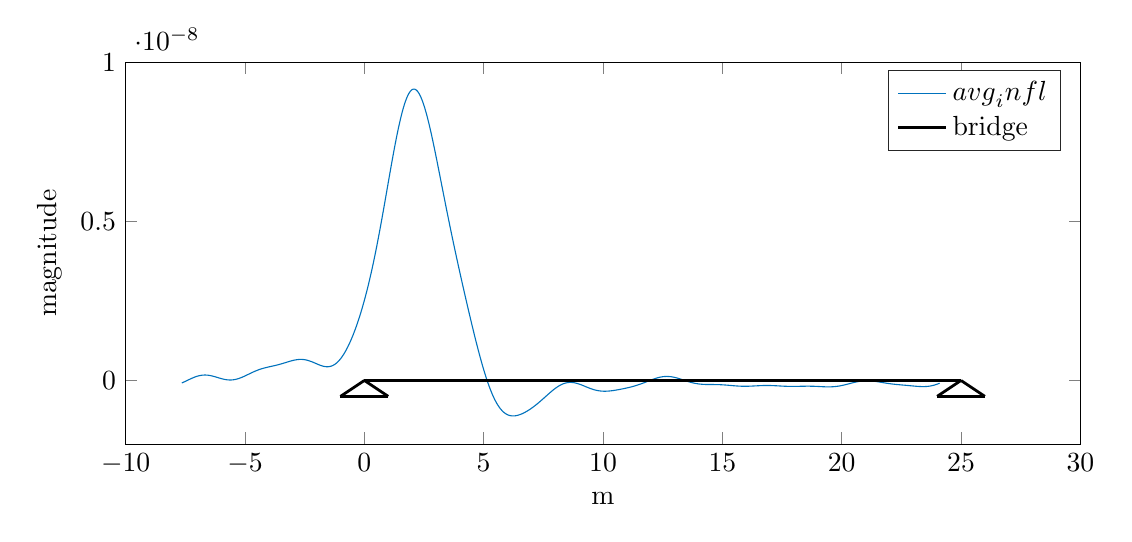
\begin{tikzpicture}

  \begin{axis}[%
    width=\textwidth,
    height=0.4\textwidth,
    at={(0\figurewidth,0\figureheight)},
    scale only axis,
    xmin=-10,
    xmax=30,
    xlabel={m},
    ymin=-2e-09,
    ymax=1e-08,
    ylabel={magnitude},
    axis background/.style={fill=white},
    title style={font=\bfseries},
    title={},
    legend style={legend cell align=left,align=left,draw=white!15!black}
    ]
    \addplot [color=mycolor1,solid]
    table[row sep=crcr]{%
    -7.64768462890625	-7.92535606122599e-11\\
    -7.62757577636719	-7.27393758131602e-11\\
    -7.60746692382813	-6.61029311463153e-11\\
    -7.58735807128906	-5.9353956845204e-11\\
    -7.56724921875	-5.25026199809192e-11\\
    -7.54714036621094	-4.55595017582371e-11\\
    -7.52703151367188	-3.85355731934499e-11\\
    -7.50692266113281	-3.1442169238249e-11\\
    -7.48681380859375	-2.42909614197359e-11\\
    -7.46670495605469	-1.7093929072314e-11\\
    -7.44659610351563	-9.86332924260852e-12\\
    -7.42648725097656	-2.61166535370269e-12\\
    -7.4063783984375	4.64834528006659e-12\\
    -7.38626954589844	1.19038049919716e-11\\
    -7.36616069335938	1.91416702552618e-11\\
    -7.34605184082031	2.63487870249472e-11\\
    -7.32594298828125	3.35119268211912e-11\\
    -7.30583413574219	4.06178234432614e-11\\
    -7.28572528320313	4.7653210200005e-11\\
    -7.26561643066406	5.46048575402506e-11\\
    -7.245507578125	6.14596109643811e-11\\
    -7.22539872558594	6.82044290964872e-11\\
    -7.20528987304688	7.48264217951845e-11\\
    -7.18518102050781	8.13128881801228e-11\\
    -7.16507216796875	8.76513544507827e-11\\
    -7.14496331542969	9.38296113738264e-11\\
    -7.12485446289063	9.98357513157788e-11\\
    -7.10474561035156	1.05658204698304e-10\\
    -7.0846367578125	1.11285775754643e-10\\
    -7.06452790527344	1.1670767746718e-10\\
    -7.04441905273438	1.21913565568231e-10\\
    -7.02431020019531	1.26893571488342e-10\\
    -7.00420134765625	1.31638334139349e-10\\
    -6.98409249511719	1.36139030422493e-10\\
    -6.96398364257813	1.40387404355548e-10\\
    -6.94387479003906	1.44375794716815e-10\\
    -6.9237659375	1.48097161108209e-10\\
    -6.90365708496094	1.51545108344237e-10\\
    -6.88354823242188	1.54713909078826e-10\\
    -6.86343937988281	1.57598524587133e-10\\
    -6.84333052734375	1.60194623625241e-10\\
    -6.82322167480469	1.62498599296469e-10\\
    -6.80311282226563	1.64507583859289e-10\\
    -6.78300396972656	1.66219461418285e-10\\
    -6.7628951171875	1.67632878446171e-10\\
    -6.74278626464844	1.68747252091946e-10\\
    -6.72267741210938	1.69562776237061e-10\\
    -6.70256855957031	1.70080425269016e-10\\
    -6.68245970703125	1.70301955548797e-10\\
    -6.66235085449219	1.70229904556411e-10\\
    -6.64224200195313	1.69867587705934e-10\\
    -6.62213314941406	1.69219092829479e-10\\
    -6.602024296875	1.68289272336779e-10\\
    -6.58191544433594	1.67083733065046e-10\\
    -6.56180659179688	1.65608823841112e-10\\
    -6.54169773925781	1.63871620785711e-10\\
    -6.52158888671875	1.61879910397012e-10\\
    -6.50148003417969	1.59642170458213e-10\\
    -6.48137118164063	1.57167548820976e-10\\
    -6.46126232910156	1.54465840123994e-10\\
    -6.4411534765625	1.51547460512574e-10\\
    -6.42104462402344	1.48423420432242e-10\\
    -6.40093577148438	1.45105295575655e-10\\
    -6.38082691894531	1.41605196068613e-10\\
    -6.36071806640625	1.37935733986815e-10\\
    -6.34060921386719	1.34109989301004e-10\\
    -6.32050036132813	1.30141474353259e-10\\
    -6.30039150878906	1.26044096972666e-10\\
    -6.28028265625	1.21832122343035e-10\\
    -6.26017380371094	1.17520133739992e-10\\
    -6.24006495117188	1.13122992258585e-10\\
    -6.21995609863281	1.08655795656361e-10\\
    -6.19984724609375	1.04133836439856e-10\\
    -6.17973839355469	9.95725593255118e-11\\
    -6.15962954101563	9.49875182080638e-11\\
    -6.13952068847656	9.03943327716995e-11\\
    -6.1194118359375	8.58086448804225e-11\\
    -6.09930298339844	8.12460748853875e-11\\
    -6.07919413085938	7.6722177987207e-11\\
    -6.05908527832031	7.22524007916065e-11\\
    -6.03897642578125	6.78520381961608e-11\\
    -6.01886757324219	6.35361907452385e-11\\
    -5.99875872070313	5.93197225887657e-11\\
    -5.97864986816406	5.52172201787717e-11\\
    -5.958541015625	5.12429518354597e-11\\
    -5.93843216308594	4.74108283117433e-11\\
    -5.91832331054688	4.37343644822523e-11\\
    -5.89821445800781	4.022664227911e-11\\
    -5.87810560546875	3.69002749929221e-11\\
    -5.85799675292969	3.37673730529439e-11\\
    -5.83788790039063	3.08395113957589e-11\\
    -5.81777904785156	2.81276985264834e-11\\
    -5.7976701953125	2.56423473711765e-11\\
    -5.77756134277344	2.33932480131226e-11\\
    -5.75745249023438	2.13895423996421e-11\\
    -5.73734363769531	1.96397010994315e-11\\
    -5.71723478515625	1.81515021838437e-11\\
    -5.69712593261719	1.69320122983511e-11\\
    -5.67701708007813	1.59875699833086e-11\\
    -5.65690822753906	1.53237712955432e-11\\
    -5.636799375	1.49454577747681e-11\\
    -5.61669052246094	1.48567067909024e-11\\
    -5.59658166992188	1.50608243004894e-11\\
    -5.57647281738281	1.55603400323443e-11\\
    -5.55636396484375	1.63570051144375e-11\\
    -5.53625511230469	1.74517921457999e-11\\
    -5.51614625976563	1.88448977091e-11\\
    -5.49603740722656	2.05357473112767e-11\\
    -5.4759285546875	2.25230027315026e-11\\
    -5.45581970214844	2.48045717475911e-11\\
    -5.43571084960938	2.73776202040208e-11\\
    -5.41560199707031	3.02385863767821e-11\\
    -5.39549314453125	3.33831975825551e-11\\
    -5.37538429199219	3.68064889721116e-11\\
    -5.35527543945313	4.0502824440507e-11\\
    -5.33516658691406	4.44659195793952e-11\\
    -5.315057734375	4.86888665899805e-11\\
    -5.29494888183594	5.31641610684278e-11\\
    -5.27484002929688	5.78837305692478e-11\\
    -5.25473117675781	6.28389648461643e-11\\
    -5.23462232421875	6.80207476642675e-11\\
    -5.21451347167969	7.34194900719996e-11\\
    -5.19440461914063	7.90251650165165e-11\\
    -5.17429576660156	8.48273431815375e-11\\
    -5.1541869140625	9.08152299225308e-11\\
    -5.13407806152344	9.69777031705913e-11\\
    -5.11396920898438	1.03303352172886e-10\\
    -5.09386035644531	1.09780516935006e-10\\
    -5.07375150390625	1.16397328227972e-10\\
    -5.05364265136719	1.23141748021056e-10\\
    -5.03353379882813	1.30001610199949e-10\\
    -5.01342494628906	1.36964661429175e-10\\
    -4.99331609375	1.44018602016992e-10\\
    -4.97320724121094	1.51151126641399e-10\\
    -4.95309838867188	1.58349964796186e-10\\
    -4.93298953613281	1.65602920817271e-10\\
    -4.91288068359375	1.72897913350967e-10\\
    -4.89277183105469	1.8022301412802e-10\\
    -4.87266297851563	1.87566485909649e-10\\
    -4.85255412597656	1.94916819474959e-10\\
    -4.8324452734375	2.02262769522412e-10\\
    -4.81233642089844	2.09593389362105e-10\\
    -4.79222756835938	2.16898064279786e-10\\
    -4.77211871582031	2.24166543458426e-10\\
    -4.75200986328125	2.31388970348269e-10\\
    -4.73190101074219	2.38555911381838e-10\\
    -4.71179215820313	2.45658382936318e-10\\
    -4.69168330566406	2.52687876451971e-10\\
    -4.671574453125	2.59636381621882e-10\\
    -4.65146560058594	2.66496407575168e-10\\
    -4.63135674804688	2.73261001983005e-10\\
    -4.61124789550781	2.79923768024267e-10\\
    -4.59113904296875	2.8647887915517e-10\\
    -4.57103019042969	2.92921091635256e-10\\
    -4.55092133789063	2.99245754770046e-10\\
    -4.53081248535156	3.05448818838871e-10\\
    -4.5107036328125	3.11526840684725e-10\\
    -4.49059478027344	3.17476986951374e-10\\
    -4.47048592773438	3.23297034961374e-10\\
    -4.45037707519531	3.28985371237197e-10\\
    -4.43026822265625	3.34540987676094e-10\\
    -4.41015937011719	3.39963475397839e-10\\
    -4.39005051757813	3.45253016292821e-10\\
    -4.36994166503906	3.50410372306376e-10\\
    -4.3498328125	3.55436872503309e-10\\
    -4.32972395996094	3.60334397964736e-10\\
    -4.30961510742188	3.6510536457712e-10\\
    -4.28950625488281	3.69752703781188e-10\\
    -4.26939740234375	3.74279841355673e-10\\
    -4.24928854980469	3.7869067431821e-10\\
    -4.22917969726563	3.82989546032411e-10\\
    -4.20907084472656	3.87181219616899e-10\\
    -4.1889619921875	3.91270849758217e-10\\
    -4.16885313964844	3.95263953035509e-10\\
    -4.14874428710938	3.99166376870336e-10\\
    -4.12863543457031	4.0298426722019e-10\\
    -4.10852658203125	4.06724035138876e-10\\
    -4.08841772949219	4.10392322331373e-10\\
    -4.06830887695313	4.1399596583441e-10\\
    -4.04820002441406	4.17541961957604e-10\\
    -4.028091171875	4.21037429622667e-10\\
    -4.00798231933594	4.24489573240791e-10\\
    -3.98787346679688	4.27905645270103e-10\\
    -3.96776461425781	4.31292908596572e-10\\
    -3.94765576171875	4.34658598882577e-10\\
    -3.92754690917969	4.38009887027838e-10\\
    -3.90743805664063	4.41353841887123e-10\\
    -3.88732920410156	4.44697393388699e-10\\
    -3.8672203515625	4.48047296196111e-10\\
    -3.84711149902344	4.51410094054412e-10\\
    -3.82700264648438	4.54792084959593e-10\\
    -3.80689379394531	4.58199287287459e-10\\
    -3.78678494140625	4.61637407014844e-10\\
    -3.76667608886719	4.65111806162564e-10\\
    -3.74656723632813	4.68627472585243e-10\\
    -3.72645838378906	4.72188991228695e-10\\
    -3.70634953125	4.75800516970369e-10\\
    -3.68624067871094	4.79465749153075e-10\\
    -3.66613182617188	4.83187907916213e-10\\
    -3.64602297363281	4.86969712422604e-10\\
    -3.62591412109375	4.90813361072303e-10\\
    -3.60580526855469	4.94720513787952e-10\\
    -3.58569641601563	4.98692276448836e-10\\
    -3.56558756347656	5.02729187543334e-10\\
    -3.5454787109375	5.06831207101621e-10\\
    -3.52536985839844	5.10997707962357e-10\\
    -3.50526100585938	5.15227469418874e-10\\
    -3.48515215332031	5.19518673281904e-10\\
    -3.46504330078125	5.23868902387237e-10\\
    -3.44493444824219	5.2827514156801e-10\\
    -3.42482559570313	5.32733781102442e-10\\
    -3.40471674316406	5.37240622639014e-10\\
    -3.384607890625	5.4179088759206e-10\\
    -3.36449903808594	5.46379227991911e-10\\
    -3.34439018554688	5.50999739764805e-10\\
    -3.32428133300781	5.55645978408919e-10\\
    -3.30417248046875	5.60310977024196e-10\\
    -3.28406362792969	5.64987266645036e-10\\
    -3.26395477539063	5.69666898816394e-10\\
    -3.24384592285156	5.74341470345697e-10\\
    -3.2237370703125	5.79002150154826e-10\\
    -3.20362821777344	5.83639708148694e-10\\
    -3.18351936523438	5.882445460094e-10\\
    -3.16341051269531	5.92806729817689e-10\\
    -3.14330166015625	5.97316024396648e-10\\
    -3.12319280761719	6.01761929265905e-10\\
    -3.10308395507813	6.0613371608854e-10\\
    -3.08297510253906	6.10420467487089e-10\\
    -3.06286625	6.14611117099734e-10\\
    -3.04275739746094	6.18694490742794e-10\\
    -3.02264854492188	6.22659348541312e-10\\
    -3.00253969238281	6.26494427885421e-10\\
    -2.98243083984375	6.30188487066846e-10\\
    -2.96232198730469	6.33730349446778e-10\\
    -2.94221313476563	6.3710894800411e-10\\
    -2.92210428222656	6.40313370110815e-10\\
    -2.9019954296875	6.43332902380205e-10\\
    -2.88188657714844	6.4615707543259e-10\\
    -2.86177772460938	6.48775708422909e-10\\
    -2.84166887207031	6.51178953174844e-10\\
    -2.82156001953125	6.53357337766971e-10\\
    -2.80145116699219	6.55301809417614e-10\\
    -2.78134231445313	6.57003776517198e-10\\
    -2.76123346191406	6.58455149659062e-10\\
    -2.741124609375	6.59648381522885e-10\\
    -2.72101575683594	6.60576505468156e-10\\
    -2.70090690429688	6.61233172699256e-10\\
    -2.68079805175781	6.61612687868116e-10\\
    -2.66068919921875	6.61710042985419e-10\\
    -2.64058034667969	6.61520949516744e-10\\
    -2.62047149414063	6.61041868545946e-10\\
    -2.60036264160156	6.60270038894379e-10\\
    -2.5802537890625	6.59203503091279e-10\\
    -2.56014493652344	6.57841131097766e-10\\
    -2.54003608398438	6.56182641694387e-10\\
    -2.51992723144531	6.54228621449899e-10\\
    -2.49981837890625	6.51980541197192e-10\\
    -2.47970952636719	6.49440769950559e-10\\
    -2.45960067382813	6.46612586207258e-10\\
    -2.43949182128906	6.43500186585142e-10\\
    -2.41938296875	6.40108691757212e-10\\
    -2.39927411621094	6.36444149653205e-10\\
    -2.37916526367188	6.32513535907674e-10\\
    -2.35905641113281	6.28324751543442e-10\\
    -2.33894755859375	6.23886617888927e-10\\
    -2.31883870605469	6.1920886873726e-10\\
    -2.29872985351563	6.14302139764776e-10\\
    -2.27862100097656	6.09177955235872e-10\\
    -2.2585121484375	6.03848712030769e-10\\
    -2.23840329589844	5.98327661041907e-10\\
    -2.21829444335938	5.92628885994042e-10\\
    -2.19818559082031	5.86767279752014e-10\\
    -2.17807673828125	5.80758518189048e-10\\
    -2.15796788574219	5.74619031696988e-10\\
    -2.13785903320313	5.68365974428209e-10\\
    -2.11775018066406	5.62017191366945e-10\\
    -2.097641328125	5.5559118333548e-10\\
    -2.07753247558594	5.49107070047976e-10\\
    -2.05742362304688	5.42584551331679e-10\\
    -2.03731477050781	5.3604386664178e-10\\
    -2.01720591796875	5.29505753002351e-10\\
    -1.99709706542969	5.22991401511395e-10\\
    -1.97698821289063	5.16522412553318e-10\\
    -1.95687936035156	5.10120749866715e-10\\
    -1.9367705078125	5.0380869361966e-10\\
    -1.91666165527344	4.9760879264825e-10\\
    -1.89655280273438	4.91543816017312e-10\\
    -1.87644395019531	4.85636704064705e-10\\
    -1.85633509765625	4.79910519092672e-10\\
    -1.83622624511719	4.74388395871017e-10\\
    -1.81611739257813	4.69093492117854e-10\\
    -1.79600854003906	4.64048939123713e-10\\
    -1.7758996875	4.59277792684657e-10\\
    -1.75579083496094	4.54802984508897e-10\\
    -1.73568198242188	4.50647274260059e-10\\
    -1.71557312988281	4.46833202397958e-10\\
    -1.69546427734375	4.43383043975196e-10\\
    -1.67535542480469	4.40318763544465e-10\\
    -1.65524657226563	4.37661971327782e-10\\
    -1.63513771972656	4.35433880794284e-10\\
    -1.6150288671875	4.33655267788496e-10\\
    -1.59492001464844	4.32346431345373e-10\\
    -1.57481116210938	4.31527156322568e-10\\
    -1.55470230957031	4.31216677973885e-10\\
    -1.53459345703125	4.31433648581019e-10\\
    -1.51448460449219	4.32196106253297e-10\\
    -1.49437575195313	4.33521445997414e-10\\
    -1.47426689941406	4.35426393151015e-10\\
    -1.454158046875	4.37926979265402e-10\\
    -1.43404919433594	4.41038520513903e-10\\
    -1.41394034179688	4.44775598693195e-10\\
    -1.39383148925781	4.49152044875492e-10\\
    -1.37372263671875	4.54180925759893e-10\\
    -1.35361378417969	4.59874532761206e-10\\
    -1.33350493164063	4.66244373864661e-10\\
    -1.31339607910156	4.73301168264612e-10\\
    -1.2932872265625	4.81054843795196e-10\\
    -1.27317837402344	4.89514537150393e-10\\
    -1.25306952148438	4.9868859688076e-10\\
    -1.23296066894531	5.08584589143551e-10\\
    -1.21285181640625	5.19209306172762e-10\\
    -1.19274296386719	5.30568777425305e-10\\
    -1.17263411132813	5.42668283349434e-10\\
    -1.15252525878906	5.5551237171156e-10\\
    -1.13241640625	5.6910487640781e-10\\
    -1.11230755371094	5.83448938677142e-10\\
    -1.09219870117188	5.98547030623509e-10\\
    -1.07208984863281	6.14400980945595e-10\\
    -1.05198099609375	6.31012002763934e-10\\
    -1.03187214355469	6.48380723426941e-10\\
    -1.01176329101563	6.66507216169446e-10\\
    -0.991654438476563	6.85391033489815e-10\\
    -0.971545585937501	7.05031242104699e-10\\
    -0.951436733398438	7.25426459333855e-10\\
    -0.931327880859376	7.46574890761434e-10\\
    -0.911219028320313	7.68474369014532e-10\\
    -0.891110175781251	7.91122393494886e-10\\
    -0.871001323242188	8.14516170895012e-10\\
    -0.850892470703125	8.38652656326412e-10\\
    -0.830783618164063	8.63528594884073e-10\\
    -0.810674765625	8.89140563468951e-10\\
    -0.790565913085938	9.15485012688087e-10\\
    -0.770457060546875	9.42558308650646e-10\\
    -0.750348208007813	9.70356774477499e-10\\
    -0.730239355468751	9.98876731341815e-10\\
    -0.710130502929688	1.02811453885888e-09\\
    -0.690021650390626	1.05806663464441e-09\\
    -0.669912797851564	1.08872957286284e-09\\
    -0.649803945312501	1.12010006158926e-09\\
    -0.629695092773439	1.15217499881224e-09\\
    -0.609586240234376	1.18495150690853e-09\\
    -0.589477387695314	1.21842696542494e-09\\
    -0.569368535156251	1.25259904200816e-09\\
    -0.549259682617188	1.28746572132876e-09\\
    -0.529150830078126	1.32302533185191e-09\\
    -0.509041977539063	1.35927657031442e-09\\
    -0.488933125000001	1.39621852377508e-09\\
    -0.468824272460938	1.43385068911301e-09\\
    -0.448715419921876	1.47217298985756e-09\\
    -0.428606567382813	1.51118579024201e-09\\
    -0.408497714843751	1.55088990638275e-09\\
    -0.388388862304688	1.59128661449545e-09\\
    -0.368280009765626	1.63237765606994e-09\\
    -0.348171157226563	1.67416523993605e-09\\
    -0.328062304687501	1.71665204116352e-09\\
    -0.307953452148438	1.75984119675036e-09\\
    -0.287844599609376	1.80373629806517e-09\\
    -0.267735747070313	1.84834138002094e-09\\
    -0.24762689453125	1.89366090696932e-09\\
    -0.227518041992188	1.9396997553164e-09\\
    -0.207409189453125	1.98646319287312e-09\\
    -0.187300336914063	2.03395685496531e-09\\
    -0.167191484375	2.08218671734071e-09\\
    -0.147082631835938	2.1311590659221e-09\\
    -0.126973779296875	2.18088046346784e-09\\
    -0.106864926757813	2.23135771321301e-09\\
    -0.0867560742187505	2.28259781957586e-09\\
    -0.0666472216796885	2.33460794602603e-09\\
    -0.0465383691406256	2.38739537022216e-09\\
    -0.0264295166015636	2.44096743653767e-09\\
    -0.00632066406250065	2.49533150610403e-09\\
    0.0137881884765614	2.55049490451131e-09\\
    0.0338970410156243	2.60646486731578e-09\\
    0.0540058935546863	2.6632484835139e-09\\
    0.0741147460937492	2.72085263715105e-09\\
    0.0942235986328122	2.77928394724204e-09\\
    0.114332451171874	2.83854870618851e-09\\
    0.134441303710937	2.8986528168859e-09\\
    0.154550156249999	2.95960172871949e-09\\
    0.174659008789062	3.02140037265554e-09\\
    0.194767861328124	3.0840530956392e-09\\
    0.214876713867187	3.14756359451582e-09\\
    0.234985566406249	3.21193484969684e-09\\
    0.255094418945312	3.27716905879501e-09\\
    0.275203271484374	3.34326757045676e-09\\
    0.295312124023437	3.41023081862167e-09\\
    0.315420976562499	3.47805825744062e-09\\
    0.335529829101562	3.54674829708492e-09\\
    0.355638681640625	3.6162982406787e-09\\
    0.375747534179687	3.68670422258615e-09\\
    0.395856386718749	3.75796114828369e-09\\
    0.415965239257813	3.83006263604484e-09\\
    0.436074091796875	3.90300096066251e-09\\
    0.456182944335937	3.9767669994298e-09\\
    0.476291796874999	4.05135018059567e-09\\
    0.496400649414062	4.12673843450675e-09\\
    0.516509501953125	4.20291814764051e-09\\
    0.536618354492187	4.27987411972828e-09\\
    0.556727207031249	4.35758952415932e-09\\
    0.576836059570312	4.43604587184907e-09\\
    0.596944912109374	4.51522297874592e-09\\
    0.617053764648436	4.59509893714175e-09\\
    0.637162617187498	4.67565009094124e-09\\
    0.657271469726562	4.75685101503482e-09\\
    0.677380322265624	4.83867449890883e-09\\
    0.697489174804686	4.92109153461512e-09\\
    0.717598027343748	5.0040713092102e-09\\
    0.737706879882812	5.08758120176172e-09\\
    0.757815732421874	5.17158678500705e-09\\
    0.777924584960936	5.2560518317358e-09\\
    0.7980334375	5.34093832595437e-09\\
    0.818142290039062	5.42620647887686e-09\\
    0.838251142578124	5.51181474977284e-09\\
    0.858359995117186	5.59771987168794e-09\\
    0.87846884765625	5.68387688203912e-09\\
    0.898577700195312	5.77023915807185e-09\\
    0.918686552734374	5.85675845715184e-09\\
    0.938795405273436	5.94338496184964e-09\\
    0.9589042578125	6.03006732976161e-09\\
    0.979013110351562	6.11675274799652e-09\\
    0.999121962890624	6.20338699224262e-09\\
    1.01923081542969	6.28991449031581e-09\\
    1.03933966796875	6.37627839007583e-09\\
    1.05944852050781	6.4624206315833e-09\\
    1.07955737304687	6.54828202335745e-09\\
    1.09966622558594	6.63380232258108e-09\\
    1.119775078125	6.71892031908669e-09\\
    1.13988393066406	6.80357392294551e-09\\
    1.15999278320312	6.88770025546942e-09\\
    1.18010163574219	6.97123574342436e-09\\
    1.20021048828125	7.05411621624324e-09\\
    1.22031934082031	7.13627700601616e-09\\
    1.24042819335937	7.21765305002616e-09\\
    1.26053704589844	7.29817899558994e-09\\
    1.2806458984375	7.37778930695472e-09\\
    1.30075475097656	7.4564183739947e-09\\
    1.32086360351562	7.53400062244427e-09\\
    1.34097245605469	7.61047062539842e-09\\
    1.36108130859375	7.68576321580608e-09\\
    1.38119016113281	7.75981359967732e-09\\
    1.40129901367188	7.83255746972173e-09\\
    1.42140786621094	7.90393111913253e-09\\
    1.44151671875	7.97387155522867e-09\\
    1.46162557128906	8.04231661266634e-09\\
    1.48173442382812	8.10920506593058e-09\\
    1.50184327636719	8.17447674081852e-09\\
    1.52195212890625	8.23807262462684e-09\\
    1.54206098144531	8.2999349747584e-09\\
    1.56216983398437	8.36000742546599e-09\\
    1.58227868652344	8.41823509245489e-09\\
    1.6023875390625	8.47456467507101e-09\\
    1.62249639160156	8.52894455580621e-09\\
    1.64260524414062	8.58132489685949e-09\\
    1.66271409667969	8.63165773349925e-09\\
    1.68282294921875	8.6798970639799e-09\\
    1.70293180175781	8.72599893577466e-09\\
    1.72304065429687	8.76992152789576e-09\\
    1.74314950683594	8.81162522908303e-09\\
    1.763258359375	8.85107271165282e-09\\
    1.78336721191406	8.88822900081014e-09\\
    1.80347606445312	8.92306153923911e-09\\
    1.82358491699219	8.95554024679893e-09\\
    1.84369376953125	8.98563757516577e-09\\
    1.86380262207031	9.01332855727426e-09\\
    1.88391147460937	9.03859085142624e-09\\
    1.90402032714844	9.06140477994866e-09\\
    1.9241291796875	9.08175336229717e-09\\
    1.94423803222656	9.09962234251686e-09\\
    1.96434688476562	9.11500021098699e-09\\
    1.98445573730469	9.1278782203918e-09\\
    2.00456458984375	9.13825039587521e-09\\
    2.02467344238281	9.14611353935308e-09\\
    2.04478229492187	9.15146722797241e-09\\
    2.06489114746094	9.15431380672281e-09\\
    2.085	9.15465837522146e-09\\
    2.10510885253906	9.15250876870854e-09\\
    2.12521770507812	9.14787553330597e-09\\
    2.14532655761719	9.14077189560757e-09\\
    2.16543541015625	9.13121372668456e-09\\
    2.18554426269531	9.11921950060484e-09\\
    2.20565311523437	9.10481024757996e-09\\
    2.22576196777344	9.08800950186764e-09\\
    2.2458708203125	9.06884324457209e-09\\
    2.26597967285156	9.04733984149802e-09\\
    2.28608852539062	9.02352997622738e-09\\
    2.30619737792969	8.99744657860065e-09\\
    2.32630623046875	8.96912474879664e-09\\
    2.34641508300781	8.93860167721649e-09\\
    2.36652393554687	8.90591656038823e-09\\
    2.38663278808594	8.87111051311908e-09\\
    2.406741640625	8.83422647713188e-09\\
    2.42685049316406	8.7953091264313e-09\\
    2.44695934570312	8.75440476965375e-09\\
    2.46706819824219	8.71156124966204e-09\\
    2.48717705078125	8.66682784065311e-09\\
    2.50728590332031	8.62025514305254e-09\\
    2.52739475585937	8.57189497647512e-09\\
    2.54750360839844	8.52180027103464e-09\\
    2.5676124609375	8.47002495728994e-09\\
    2.58772131347656	8.41662385511651e-09\\
    2.60783016601562	8.36165256179487e-09\\
    2.62793901855469	8.30516733960799e-09\\
    2.64804787109375	8.24722500323978e-09\\
    2.66815672363281	8.18788280726605e-09\\
    2.68826557617188	8.12719833402794e-09\\
    2.70837442871094	8.06522938217475e-09\\
    2.72848328125	8.0020338561603e-09\\
    2.74859213378906	7.93766965697282e-09\\
    2.76870098632812	7.87219457437286e-09\\
    2.78880983886719	7.80566618090885e-09\\
    2.80891869140625	7.73814172797259e-09\\
    2.82902754394531	7.66967804415044e-09\\
    2.84913639648437	7.60033143611745e-09\\
    2.86924524902344	7.53015759231338e-09\\
    2.8893541015625	7.45921148963014e-09\\
    2.90946295410156	7.38754730333008e-09\\
    2.92957180664062	7.31521832040425e-09\\
    2.94968065917969	7.24227685656836e-09\\
    2.96978951171875	7.16877417708276e-09\\
    2.98989836425781	7.09476042157034e-09\\
    3.01000721679687	7.0202845329938e-09\\
    3.03011606933594	6.94539419094069e-09\\
    3.050224921875	6.87013574935113e-09\\
    3.07033377441406	6.79455417880937e-09\\
    3.09044262695312	6.71869301350652e-09\\
    3.11055147949219	6.64259430296704e-09\\
    3.13066033203125	6.56629856861773e-09\\
    3.15076918457031	6.48984476526265e-09\\
    3.17087803710937	6.4132702475132e-09\\
    3.19098688964844	6.33661074120743e-09\\
    3.2110957421875	6.25990031983795e-09\\
    3.23120459472656	6.18317138599294e-09\\
    3.25131344726562	6.10645465780018e-09\\
    3.27142229980469	6.02977916034909e-09\\
    3.29153115234375	5.95317222205177e-09\\
    3.31164000488281	5.87665947588917e-09\\
    3.33174885742187	5.80026486547524e-09\\
    3.35185770996094	5.72401065585754e-09\\
    3.3719665625	5.64791744895984e-09\\
    3.39207541503906	5.57200420355908e-09\\
    3.41218426757812	5.49628825967643e-09\\
    3.43229312011719	5.42078536725019e-09\\
    3.45240197265625	5.34550971894645e-09\\
    3.47251082519531	5.27047398695231e-09\\
    3.49261967773437	5.19568936358612e-09\\
    3.51272853027344	5.1211656055487e-09\\
    3.5328373828125	5.04691108163057e-09\\
    3.55294623535156	4.9729328236812e-09\\
    3.57305508789062	4.89923658063819e-09\\
    3.59316394042969	4.82582687540696e-09\\
    3.61327279296875	4.75270706437469e-09\\
    3.63338164550781	4.67987939933632e-09\\
    3.65349049804687	4.607345091605e-09\\
    3.67359935058594	4.53510437807515e-09\\
    3.693708203125	4.46315658900201e-09\\
    3.71381705566406	4.39150021725908e-09\\
    3.73392590820312	4.32013298883218e-09\\
    3.75403476074219	4.24905193430764e-09\\
    3.77414361328125	4.17825346111124e-09\\
    3.79425246582031	4.10773342625467e-09\\
    3.81436131835937	4.03748720934715e-09\\
    3.83447017089844	3.96750978563127e-09\\
    3.8545790234375	3.89779579880454e-09\\
    3.87468787597656	3.82833963339124e-09\\
    3.89479672851562	3.75913548643276e-09\\
    3.91490558105469	3.69017743826934e-09\\
    3.93501443359375	3.62145952219111e-09\\
    3.95512328613281	3.55297579274219e-09\\
    3.97523213867188	3.48472039246818e-09\\
    3.99534099121094	3.41668761690437e-09\\
    4.01544984375	3.34887197760966e-09\\
    4.03555869628906	3.2812682630596e-09\\
    4.05566754882812	3.21387159722053e-09\\
    4.07577640136719	3.1466774956361e-09\\
    4.09588525390625	3.07968191886748e-09\\
    4.11599410644531	3.01288132313823e-09\\
    4.13610295898437	2.946272708046e-09\\
    4.15621181152344	2.87985366121357e-09\\
    4.1763206640625	2.81362239976339e-09\\
    4.19642951660156	2.74757780851131e-09\\
    4.21653836914062	2.68171947478667e-09\\
    4.23664722167969	2.61604771979822e-09\\
    4.25675607421875	2.55056362647754e-09\\
    4.27686492675781	2.4852690637435e-09\\
    4.29697377929687	2.42016670714416e-09\\
    4.31708263183594	2.35526005584462e-09\\
    4.337191484375	2.29055344594181e-09\\
    4.35730033691406	2.22605206009964e-09\\
    4.37740918945312	2.16176193351013e-09\\
    4.39751804199219	2.09768995619834e-09\\
    4.41762689453125	2.03384387170103e-09\\
    4.43773574707031	1.97023227216064e-09\\
    4.45784459960937	1.90686458988786e-09\\
    4.47795345214844	1.84375108545743e-09\\
    4.4980623046875	1.78090283241257e-09\\
    4.51817115722656	1.71833169866454e-09\\
    4.53828000976562	1.65605032468357e-09\\
    4.55838886230469	1.59407209858785e-09\\
    4.57849771484375	1.53241112824628e-09\\
    4.59860656738281	1.47108221051997e-09\\
    4.61871541992187	1.41010079777579e-09\\
    4.63882427246094	1.34948296181336e-09\\
    4.658933125	1.28924535535435e-09\\
    4.67904197753906	1.22940517124974e-09\\
    4.69915083007812	1.1699800995671e-09\\
    4.71925968261719	1.11098828272568e-09\\
    4.73936853515625	1.05244826885213e-09\\
    4.75947738769531	9.94378963534237e-10\\
    4.77958624023437	9.36799580153915e-10\\
    4.79969509277344	8.79729588983905e-10\\
    4.8198039453125	8.23188665235164e-10\\
    4.83991279785156	7.67196636243921e-10\\
    4.86002165039062	7.11773427988616e-10\\
    4.88013050292969	6.5693901112749e-10\\
    4.90023935546875	6.02713346747707e-10\\
    4.92034820800781	5.49116332016033e-10\\
    4.94045706054687	4.96167745919958e-10\\
    4.96056591308594	4.43887195286001e-10\\
    4.980674765625	3.92294061259612e-10\\
    5.00078361816406	3.41407446427651e-10\\
    5.02089247070312	2.91246122760918e-10\\
    5.04100132324219	2.41828480549654e-10\\
    5.06111017578125	1.93172478500218e-10\\
    5.08121902832031	1.4529559515559e-10\\
    5.10132788085937	9.82147817965328e-11\\
    5.12143673339844	5.19464169736976e-11\\
    5.1415455859375	6.50626281422238e-12\\
    5.16165443847656	-3.80905767611195e-11\\
    5.18176329101562	-8.18296957817e-11\\
    5.20187214355469	-1.24697423811525e-10\\
    5.22198099609375	-1.66680861262484e-10\\
    5.24208984863281	-2.07767912333342e-10\\
    5.26219870117187	-2.47947315480364e-10\\
    5.28230755371094	-2.87208671334902e-10\\
    5.30241640625	-3.25542467992676e-10\\
    5.32252525878906	-3.62940103609296e-10\\
    5.34263411132812	-3.99393906246303e-10\\
    5.36274296386719	-4.34897150922132e-10\\
    5.38285181640625	-4.69444073832248e-10\\
    5.40296066894531	-5.0302988371301e-10\\
    5.42306952148437	-5.356507703337e-10\\
    5.44317837402344	-5.67303910111425e-10\\
    5.4632872265625	-5.97987468853416e-10\\
    5.48339607910156	-6.27700601641335e-10\\
    5.50350493164062	-6.56443449881822e-10\\
    5.52361378417969	-6.8421713555728e-10\\
    5.54372263671875	-7.11023752720182e-10\\
    5.56383148925781	-7.36866356283494e-10\\
    5.58394034179687	-7.61748948168678e-10\\
    5.60404919433594	-7.85676460881427e-10\\
    5.624158046875	-8.08654738593589e-10\\
    5.64426689941406	-8.30690515817797e-10\\
    5.66437575195312	-8.51791393768871e-10\\
    5.68448460449219	-8.71965814513392e-10\\
    5.70459345703125	-8.91223033015561e-10\\
    5.72470230957031	-9.09573087194e-10\\
    5.74481116210937	-9.27026766109902e-10\\
    5.76492001464844	-9.43595576412612e-10\\
    5.7850288671875	-9.59291707173499e-10\\
    5.80513771972656	-9.74127993243622e-10\\
    5.82524657226562	-9.88117877274542e-10\\
    5.84535542480469	-1.00127537054515e-09\\
    5.86546427734375	-1.01361501274021e-09\\
    5.88557312988281	-1.02515183082875e-09\\
    5.90568198242187	-1.03590129719227e-09\\
    5.92579083496094	-1.04587928715382e-09\\
    5.9458996875	-1.0551020360601e-09\\
    5.96600854003906	-1.06358609606847e-09\\
    5.98611739257812	-1.07134829279075e-09\\
    6.00622624511719	-1.07840568194463e-09\\
    6.02633509765625	-1.08477550616199e-09\\
    6.04644395019531	-1.09047515210173e-09\\
    6.06655280273437	-1.09552210801197e-09\\
    6.08666165527344	-1.09993392188359e-09\\
    6.1067705078125	-1.10372816033381e-09\\
    6.12687936035156	-1.10692236835418e-09\\
    6.14698821289062	-1.10953403005337e-09\\
    6.16709706542969	-1.1115805305201e-09\\
    6.18720591796875	-1.11307911892633e-09\\
    6.20731477050781	-1.11404687298521e-09\\
    6.22742362304687	-1.11450066487242e-09\\
    6.24753247558594	-1.11445712871288e-09\\
    6.267641328125	-1.11393262972851e-09\\
    6.28775018066406	-1.11294323513529e-09\\
    6.30785903320312	-1.1115046868712e-09\\
    6.32796788574219	-1.10963237622846e-09\\
    6.34807673828125	-1.10734132045648e-09\\
    6.36818559082031	-1.10464614139343e-09\\
    6.38829444335937	-1.10156104617678e-09\\
    6.40840329589844	-1.09809981007458e-09\\
    6.4285121484375	-1.09427576147146e-09\\
    6.44862100097656	-1.0901017690344e-09\\
    6.46872985351562	-1.08559023107568e-09\\
    6.48883870605469	-1.08075306712124e-09\\
    6.50894755859375	-1.0756017116851e-09\\
    6.52905641113281	-1.07014711024176e-09\\
    6.54916526367187	-1.06439971738028e-09\\
    6.56927411621094	-1.05836949711596e-09\\
    6.58938296875	-1.05206592532734e-09\\
    6.60949182128906	-1.04549799427848e-09\\
    6.62960067382812	-1.03867421917916e-09\\
    6.64970952636719	-1.03160264672788e-09\\
    6.66981837890625	-1.02429086557585e-09\\
    6.68992723144531	-1.01674601864305e-09\\
    6.71003608398437	-1.0089748172111e-09\\
    6.73014493652344	-1.00098355671134e-09\\
    6.7502537890625	-9.92778134120753e-10\\
    6.77036264160156	-9.84364066872842e-10\\
    6.79047149414062	-9.75746513185355e-10\\
    6.81058034667969	-9.66930293702193e-10\\
    6.83068919921875	-9.5791991434237e-10\\
    6.85079805175781	-9.48719590245079e-10\\
    6.87090690429687	-9.39333270696392e-10\\
    6.89101575683594	-9.29764664920247e-10\\
    6.911124609375	-9.20017268613583e-10\\
    6.93123346191406	-9.10094391103689e-10\\
    6.95134231445312	-8.99999183003911e-10\\
    6.97145116699219	-8.89734664242932e-10\\
    6.99156001953125	-8.79303752342029e-10\\
    7.01166887207031	-8.68709290814548e-10\\
    7.03177772460937	-8.57954077562084e-10\\
    7.05188657714844	-8.47040893142631e-10\\
    7.0719954296875	-8.35972528787055e-10\\
    7.09210428222656	-8.24751814042053e-10\\
    7.11221313476562	-8.13381643919686e-10\\
    7.13232198730469	-8.01865005436296e-10\\
    7.15243083984375	-7.9020500342639e-10\\
    7.17253969238281	-7.7840488552068e-10\\
    7.19264854492187	-7.6646806618102e-10\\
    7.21275739746094	-7.54398149689382e-10\\
    7.23286625	-7.42198951992313e-10\\
    7.25297510253906	-7.2987452130749e-10\\
    7.27308395507812	-7.17429157403869e-10\\
    7.29319280761719	-7.04867429472825e-10\\
    7.31330166015625	-6.92194192513147e-10\\
    7.33341051269531	-6.79414602159151e-10\\
    7.35351936523437	-6.66534127887227e-10\\
    7.37362821777344	-6.53558564542937e-10\\
    7.3937370703125	-6.40494042137314e-10\\
    7.41384592285156	-6.27347033868047e-10\\
    7.43395477539062	-6.14124362328246e-10\\
    7.45406362792969	-6.00833203872694e-10\\
    7.47417248046875	-5.87481091118624e-10\\
    7.49428133300781	-5.74075913565593e-10\\
    7.51439018554687	-5.60625916326152e-10\\
    7.53449903808594	-5.47139696966558e-10\\
    7.554607890625	-5.33626200463984e-10\\
    7.57471674316406	-5.20094712294117e-10\\
    7.59482559570312	-5.06554849670089e-10\\
    7.61493444824219	-4.93016550961026e-10\\
    7.63504330078125	-4.79490063325283e-10\\
    7.65515215332031	-4.65985928600494e-10\\
    7.67526100585937	-4.52514967499071e-10\\
    7.69536985839844	-4.3908826216442e-10\\
    7.7154787109375	-4.25717137149265e-10\\
    7.73558756347656	-4.12413138883635e-10\\
    7.75569641601562	-3.99188013705657e-10\\
    7.77580526855469	-3.86053684533957e-10\\
    7.79591412109375	-3.73022226265452e-10\\
    7.81602297363281	-3.60105839987313e-10\\
    7.83613182617187	-3.47316826096265e-10\\
    7.85624067871094	-3.34667556422652e-10\\
    7.87634953125	-3.2217044546036e-10\\
    7.89645838378906	-3.0983792080723e-10\\
    7.91656723632812	-2.97682392923458e-10\\
    7.93667608886719	-2.85716224318237e-10\\
    7.95678494140625	-2.73951698276953e-10\\
    7.97689379394531	-2.62400987243167e-10\\
    7.99700264648437	-2.51076120970838e-10\\
    8.01711149902344	-2.39988954563318e-10\\
    8.0372203515625	-2.29151136516017e-10\\
    8.05732920410156	-2.18574076879827e-10\\
    8.07743805664062	-2.08268915661986e-10\\
    8.09754690917969	-1.98246491580276e-10\\
    8.11765576171875	-1.88517311285305e-10\\
    8.13776461425781	-1.79091519163943e-10\\
    8.15787346679688	-1.69978867835026e-10\\
    8.17798231933594	-1.61188689445957e-10\\
    8.198091171875	-1.52729867876055e-10\\
    8.21820002441406	-1.44610811949306e-10\\
    8.23830887695312	-1.3683942975559e-10\\
    8.25841772949219	-1.29423104175565e-10\\
    8.27852658203125	-1.22368669700126e-10\\
    8.29863543457031	-1.15682390630769e-10\\
    8.31874428710938	-1.09369940742358e-10\\
    8.33885313964844	-1.03436384484564e-10\\
    8.3589619921875	-9.78861597928621e-11\\
    8.37907084472656	-9.27230625742782e-11\\
    8.39917969726562	-8.79502329271875e-11\\
    8.41928854980469	-8.35701431483077e-11\\
    8.43939740234375	-7.95845875738569e-11\\
    8.45950625488281	-7.59946742952503e-11\\
    8.47961510742187	-7.28008187832891e-11\\
    8.49972395996094	-7.0002739447955e-11\\
    8.5198328125	-6.75994551543151e-11\\
    8.53994166503906	-6.55892847080175e-11\\
    8.56005051757812	-6.3969848317194e-11\\
    8.58015937011719	-6.27380710305233e-11\\
    8.60026822265625	-6.18901881444559e-11\\
    8.62037707519531	-6.14217525657282e-11\\
    8.64048592773437	-6.1327644108545e-11\\
    8.66059478027343	-6.16020806990845e-11\\
    8.6807036328125	-6.22386314534934e-11\\
    8.70081248535156	-6.32302315890123e-11\\
    8.72092133789062	-6.45691991216642e-11\\
    8.74103019042969	-6.62472532977915e-11\\
    8.76113904296875	-6.8255534700865e-11\\
    8.78124789550781	-7.05846269692634e-11\\
    8.80135674804687	-7.32245800553454e-11\\
    8.82146560058593	-7.61649349508752e-11\\
    8.841574453125	-7.93947497990549e-11\\
    8.86168330566406	-8.29026273087137e-11\\
    8.88179215820312	-8.66767433819952e-11\\
    8.90190101074219	-9.07048768628159e-11\\
    8.92200986328125	-9.497444030984e-11\\
    8.94211871582031	-9.9472511694309e-11\\
    8.96222756835937	-1.04185866920247e-10\\
    8.98233642089843	-1.09101013061932e-10\\
    9.0024452734375	-1.14204222211359e-10\\
    9.02255412597656	-1.19481565826673e-10\\
    9.04266297851562	-1.24918949471073e-10\\
    9.06277183105469	-1.30502147830728e-10\\
    9.08288068359375	-1.36216839899608e-10\\
    9.10298953613281	-1.42048644218926e-10\\
    9.12309838867187	-1.47983154059078e-10\\
    9.14320724121093	-1.54005972432487e-10\\
    9.16331609375	-1.60102746826811e-10\\
    9.18342494628906	-1.66259203549231e-10\\
    9.20353379882812	-1.72461181574354e-10\\
    9.22364265136719	-1.78694665790319e-10\\
    9.24375150390625	-1.84945819540156e-10\\
    9.26386035644531	-1.91201016358353e-10\\
    9.28396920898437	-1.97446870805654e-10\\
    9.30407806152343	-2.03670268308679e-10\\
    9.3241869140625	-2.09858393914736e-10\\
    9.34429576660156	-2.15998759876389e-10\\
    9.36440461914062	-2.22079231984618e-10\\
    9.38451347167969	-2.28088054574228e-10\\
    9.40462232421875	-2.34013874129996e-10\\
    9.42473117675781	-2.39845761427295e-10\\
    9.44484002929687	-2.45573232146167e-10\\
    9.46494888183594	-2.51186265903594e-10\\
    9.485057734375	-2.56675323654283e-10\\
    9.50516658691406	-2.62031363416261e-10\\
    9.52527543945312	-2.67245854283629e-10\\
    9.54538429199219	-2.7231078869488e-10\\
    9.56549314453125	-2.77218692931526e-10\\
    9.58560199707031	-2.81962635827931e-10\\
    9.60571084960937	-2.86536235679711e-10\\
    9.62581970214844	-2.90933665344337e-10\\
    9.6459285546875	-2.95149655533889e-10\\
    9.66603740722656	-2.9917949630634e-10\\
    9.68614625976562	-3.03019036767877e-10\\
    9.70625511230469	-3.06664683005067e-10\\
    9.72636396484375	-3.10113394271688e-10\\
    9.74647281738281	-3.13362677461125e-10\\
    9.76658166992187	-3.16410579900925e-10\\
    9.78669052246094	-3.19255680511985e-10\\
    9.806799375	-3.21897079380137e-10\\
    9.82690822753906	-3.24334385793419e-10\\
    9.84701708007812	-3.26567704803195e-10\\
    9.86712593261719	-3.28597622372365e-10\\
    9.88723478515625	-3.30425189178311e-10\\
    9.90734363769531	-3.32051903142748e-10\\
    9.92745249023437	-3.33479690764524e-10\\
    9.94756134277344	-3.34710887335408e-10\\
    9.9676701953125	-3.35748216122096e-10\\
    9.98777904785156	-3.36594766601083e-10\\
    10.0078879003906	-3.37253971835611e-10\\
    10.0279967529297	-3.3772958508658e-10\\
    10.0481056054687	-3.38025655751286e-10\\
    10.0682144580078	-3.38146504725755e-10\\
    10.0883233105469	-3.38096699287733e-10\\
    10.1084321630859	-3.37881027598583e-10\\
    10.128541015625	-3.3750447292292e-10\\
    10.1486498681641	-3.36972187665233e-10\\
    10.1687587207031	-3.36289467322652e-10\\
    10.1888675732422	-3.3546172445267e-10\\
    10.2089764257812	-3.34494462753806e-10\\
    10.2290852783203	-3.33393251356177e-10\\
    10.2491941308594	-3.32163699417383e-10\\
    10.2693029833984	-3.30811431117382e-10\\
    10.2894118359375	-3.29342061143835e-10\\
    10.3095206884766	-3.27761170756975e-10\\
    10.3296295410156	-3.26074284520188e-10\\
    10.3497383935547	-3.24286847779536e-10\\
    10.3698472460937	-3.22404204971887e-10\\
    10.3899560986328	-3.20431578837826e-10\\
    10.4100649511719	-3.18374050611453e-10\\
    10.4301738037109	-3.16236541255086e-10\\
    10.45028265625	-3.14023793802386e-10\\
    10.4703915087891	-3.11740356868885e-10\\
    10.4905003613281	-3.09390569384001e-10\\
    10.5106092138672	-3.06978546593581e-10\\
    10.5307180664062	-3.04508167376979e-10\\
    10.5508269189453	-3.01983062917179e-10\\
    10.5709357714844	-2.99406606757197e-10\\
    10.5910446240234	-2.96781906270338e-10\\
    10.6111534765625	-2.9411179556637e-10\\
    10.6312623291016	-2.91398829849887e-10\\
    10.6513711816406	-2.88645281241558e-10\\
    10.6714800341797	-2.85853136067052e-10\\
    10.6915888867187	-2.83024093612917e-10\\
    10.7116977392578	-2.80159566342726e-10\\
    10.7318065917969	-2.77260681561446e-10\\
    10.7519154443359	-2.74328284510089e-10\\
    10.772024296875	-2.71362942867497e-10\\
    10.7921331494141	-2.68364952630443e-10\\
    10.8122420019531	-2.6533434533823e-10\\
    10.8323508544922	-2.62270896602594e-10\\
    10.8524597070312	-2.59174135899001e-10\\
    10.8725685595703	-2.56043357570436e-10\\
    10.8926774121094	-2.52877632990432e-10\\
    10.9127862646484	-2.49675823827498e-10\\
    10.9328951171875	-2.4643659634921e-10\\
    10.9530039697266	-2.4315843670017e-10\\
    10.9731128222656	-2.3983966708454e-10\\
    10.9932216748047	-2.36478462780448e-10\\
    11.0133305273437	-2.33072869910551e-10\\
    11.0334393798828	-2.2962082389025e-10\\
    11.0535482324219	-2.26120168472588e-10\\
    11.0736570849609	-2.22568675306758e-10\\
    11.0937659375	-2.18964063925289e-10\\
    11.1138747900391	-2.15304022073464e-10\\
    11.1339836425781	-2.11586226293447e-10\\
    11.1540924951172	-2.07808362674621e-10\\
    11.1742013476562	-2.03968147681305e-10\\
    11.1943102001953	-2.00063348968727e-10\\
    11.2144190527344	-1.96091806098399e-10\\
    11.2345279052734	-1.92051451064508e-10\\
    11.2546367578125	-1.87940328543825e-10\\
    11.2747456103516	-1.83756615782794e-10\\
    11.2948544628906	-1.79498642036958e-10\\
    11.3149633154297	-1.75164907479763e-10\\
    11.3350721679687	-1.70754101499812e-10\\
    11.3551810205078	-1.66265120308224e-10\\
    11.3752898730469	-1.61697083780324e-10\\
    11.3953987255859	-1.57049351459047e-10\\
    11.415507578125	-1.52321537650619e-10\\
    11.4356164306641	-1.47513525546694e-10\\
    11.4557252832031	-1.42625480310848e-10\\
    11.4758341357422	-1.37657861071413e-10\\
    11.4959429882812	-1.32611431766798e-10\\
    11.5160518408203	-1.27487270793933e-10\\
    11.5361606933594	-1.22286779415018e-10\\
    11.5562695458984	-1.17011688882633e-10\\
    11.5763783984375	-1.11664066248019e-10\\
    11.5964872509766	-1.06246318822612e-10\\
    11.6165961035156	-1.00761197267826e-10\\
    11.6367049560547	-9.52117972935632e-11\\
    11.6568138085938	-8.96015599510086e-11\\
    11.6769226611328	-8.39342705108838e-11\\
    11.6970315136719	-7.82140559234927e-11\\
    11.7171403662109	-7.24453808624598e-11\\
    11.73724921875	-6.66330423594254e-11\\
    11.7573580712891	-6.07821630422604e-11\\
    11.7774669238281	-5.4898182994774e-11\\
    11.7975757763672	-4.89868502610858e-11\\
    11.8176846289063	-4.30542100230089e-11\\
    11.8377934814453	-3.7106592483821e-11\\
    11.8579023339844	-3.11505994967964e-11\\
    11.8780111865234	-2.51930899815499e-11\\
    11.8981200390625	-1.92411641759935e-11\\
    11.9182288916016	-1.33021467760283e-11\\
    11.9383377441406	-7.38356901944579e-12\\
    11.9584465966797	-1.49314977449635e-12\\
    11.9785554492187	4.36122430257299e-12\\
    11.9986643017578	1.0171519473149e-11\\
    12.0187731542969	1.59295764138208e-11\\
    12.0388820068359	2.16271324316341e-11\\
    12.058990859375	2.72558443199693e-11\\
    12.0790997119141	3.28073117754438e-11\\
    12.0992085644531	3.8273101294039e-11\\
    12.1193174169922	4.36447704628036e-11\\
    12.1394262695312	4.89138925616999e-11\\
    12.1595351220703	5.40720813890738e-11\\
    12.1796439746094	5.91110162230853e-11\\
    12.1997528271484	6.40224668308491e-11\\
    12.2198616796875	6.87983184366728e-11\\
    12.2399705322266	7.34305965608041e-11\\
    12.2600793847656	7.79114916403085e-11\\
    12.2801882373047	8.2233383344469e-11\\
    12.3002970898437	8.63888644978782e-11\\
    12.3204059423828	9.03707645258351e-11\\
    12.3405147949219	9.41721723380537e-11\\
    12.3606236474609	9.77864585687184e-11\\
    12.3807325	1.01207297092966e-10\\
    12.4008413525391	1.04428685742448e-10\\
    12.4209502050781	1.07444966145259e-10\\
    12.4410590576172	1.10250842618619e-10\\
    12.4611679101562	1.12841400045899e-10\\
    12.4812767626953	1.15212120673124e-10\\
    12.5013856152344	1.17358899763832e-10\\
    12.5214944677734	1.19278060055087e-10\\
    12.5416033203125	1.20966364961718e-10\\
    12.5617121728516	1.22421030480037e-10\\
    12.5818210253906	1.23639735747052e-10\\
    12.6019298779297	1.24620632215618e-10\\
    12.6220387304687	1.25362351411039e-10\\
    12.6421475830078	1.25864011239371e-10\\
    12.6622564355469	1.26125220822903e-10\\
    12.6823652880859	1.26146083843257e-10\\
    12.702474140625	1.2592720037795e-10\\
    12.7225829931641	1.25469667221275e-10\\
    12.7426918457031	1.2477507668587e-10\\
    12.7628006982422	1.23845513886433e-10\\
    12.7829095507812	1.22683552512487e-10\\
    12.8030184033203	1.21292249102191e-10\\
    12.8231272558594	1.1967513583454e-10\\
    12.8432361083984	1.17836211862317e-10\\
    12.8633449609375	1.15779933213306e-10\\
    12.8834538134766	1.13511201292116e-10\\
    12.9035626660156	1.11035350019962e-10\\
    12.9236715185547	1.08358131654207e-10\\
    12.9437803710937	1.05485701334263e-10\\
    12.9638892236328	1.02424600404593e-10\\
    12.9839980761719	9.91817385699299e-11\\
    13.0041069287109	9.57643749416215e-11\\
    13.02421578125	9.21800980379785e-11\\
    13.0443246337891	8.84368048048506e-11\\
    13.0644334863281	8.45426787261383e-11\\
    13.0845423388672	8.05061670968192e-11\\
    13.1046511914062	7.63359575340422e-11\\
    13.1247600439453	7.204095380419e-11\\
    13.1448688964844	6.76302510461875e-11\\
    13.1649777490234	6.31131104731657e-11\\
    13.1850866015625	5.84989336363933e-11\\
    13.2051954541016	5.37972363365596e-11\\
    13.2253043066406	4.90176222687698e-11\\
    13.2454131591797	4.4169756488117e-11\\
    13.2655220117187	3.92633387834226e-11\\
    13.2856308642578	3.43080770465567e-11\\
    13.3057397167969	2.93136607248577e-11\\
    13.3258485693359	2.42897344435007e-11\\
    13.345957421875	1.92458718839231e-11\\
    13.3660662744141	1.41915500034065e-11\\
    13.3861751269531	9.1361236793597e-12\\
    13.4062839794922	4.08880086035198e-12\\
    13.4263928320312	-9.41381696181604e-13\\
    13.4465016845703	-5.94558202174408e-12\\
    13.4666105371094	-1.09151757949226e-11\\
    13.4867193896484	-1.58417783873181e-11\\
    13.5068282421875	-2.07172660279059e-11\\
    13.5269370947266	-2.55337960195189e-11\\
    13.5470459472656	-3.02838259448546e-11\\
    13.5671547998047	-3.49601318028615e-11\\
    13.5872636523437	-3.95558250204761e-11\\
    13.6073725048828	-4.40643682885443e-11\\
    13.6274813574219	-4.84795901752014e-11\\
    13.6475902099609	-5.27956984741922e-11\\
    13.6676990625	-5.70072922502989e-11\\
    13.6878079150391	-6.11093725485603e-11\\
    13.7079167675781	-6.50973517388688e-11\\
    13.7280256201172	-6.89670614721662e-11\\
    13.7481344726562	-7.27147592296046e-11\\
    13.7682433251953	-7.63371334507681e-11\\
    13.7883521777344	-7.98313072321979e-11\\
    13.8084610302734	-8.31948405923957e-11\\
    13.8285698828125	-8.64257313044588e-11\\
    13.8486787353516	-8.95224143025529e-11\\
    13.8687875878906	-9.24837596732552e-11\\
    13.8888964404297	-9.53090692477981e-11\\
    13.9090052929687	-9.79980718159258e-11\\
    13.9291141455078	-1.00550916986887e-10\\
    13.9492229980469	-1.02968167727632e-10\\
    13.9693318505859	-1.05250791612758e-10\\
    13.989440703125	-1.07400150825137e-10\\
    14.0095495556641	-1.0941799095025e-10\\
    14.0296584082031	-1.11306428611362e-10\\
    14.0497672607422	-1.1306793799642e-10\\
    14.0698761132812	-1.14705336331216e-10\\
    14.0899849658203	-1.16221768356793e-10\\
    14.1100938183594	-1.17620689872193e-10\\
    14.1302026708984	-1.18905850406757e-10\\
    14.1503115234375	-1.20081275088708e-10\\
    14.1704203759766	-1.21151245779411e-10\\
    14.1905292285156	-1.22120281544772e-10\\
    14.2106380810547	-1.22993118537293e-10\\
    14.2307469335937	-1.23774689363852e-10\\
    14.2508557861328	-1.24470102015806e-10\\
    14.2709646386719	-1.25084618439006e-10\\
    14.2910734912109	-1.25623632822218e-10\\
    14.31118234375	-1.26092649682941e-10\\
    14.3312911962891	-1.26497261829912e-10\\
    14.3514000488281	-1.26843128281483e-10\\
    14.3715089013672	-1.27135952218814e-10\\
    14.3916177539063	-1.27381459052146e-10\\
    14.4117266064453	-1.27585374677596e-10\\
    14.4318354589844	-1.27753404000708e-10\\
    14.4519443115234	-1.27891209801594e-10\\
    14.4720531640625	-1.28004392014724e-10\\
    14.4921620166016	-1.28098467494629e-10\\
    14.5122708691406	-1.28178850336373e-10\\
    14.5323797216797	-1.28250832817326e-10\\
    14.5524885742187	-1.28319567024133e-10\\
    14.5725974267578	-1.28390047225675e-10\\
    14.5927062792969	-1.28467093050015e-10\\
    14.6128151318359	-1.28555333519686e-10\\
    14.632923984375	-1.28659191996487e-10\\
    14.6530328369141	-1.28782872083082e-10\\
    14.6731416894531	-1.28930344525024e-10\\
    14.6932505419922	-1.29105335152786e-10\\
    14.7133593945312	-1.29311313899371e-10\\
    14.7334682470703	-1.29551484924792e-10\\
    14.7535770996094	-1.29828777874579e-10\\
    14.7736859521484	-1.30145840294909e-10\\
    14.7937948046875	-1.30505031222747e-10\\
    14.8139036572266	-1.30908415964699e-10\\
    14.8340125097656	-1.31357762074009e-10\\
    14.8541213623047	-1.31854536530383e-10\\
    14.8742302148437	-1.32399904123056e-10\\
    14.8943390673828	-1.32994727032803e-10\\
    14.9144479199219	-1.33639565604385e-10\\
    14.9345567724609	-1.34334680296299e-10\\
    14.954665625	-1.35080034790587e-10\\
    14.9747744775391	-1.35875300241061e-10\\
    14.9948833300781	-1.367198606343e-10\\
    15.0149921826172	-1.37612819233644e-10\\
    15.0351010351562	-1.38553006072652e-10\\
    15.0552098876953	-1.3953898646061e-10\\
    15.0753187402344	-1.40569070459237e-10\\
    15.0954275927734	-1.41641323286214e-10\\
    15.1155364453125	-1.42753576598029e-10\\
    15.1356452978516	-1.43903440601491e-10\\
    15.1557541503906	-1.45088316940605e-10\\
    15.1758630029297	-1.46305412302672e-10\\
    15.1959718554687	-1.47551752685328e-10\\
    15.2160807080078	-1.48824198263883e-10\\
    15.2361895605469	-1.50119458796544e-10\\
    15.2562984130859	-1.51434109503326e-10\\
    15.276407265625	-1.52764607353183e-10\\
    15.2965161181641	-1.54107307692539e-10\\
    15.3166249707031	-1.55458481147673e-10\\
    15.3367338232422	-1.56814330732647e-10\\
    15.3568426757812	-1.58171009094161e-10\\
    15.3769515283203	-1.59524635824532e-10\\
    15.3970603808594	-1.60871314774208e-10\\
    15.4171692333984	-1.62207151295602e-10\\
    15.4372780859375	-1.6352826935063e-10\\
    15.4573869384766	-1.64830828415434e-10\\
    15.4774957910156	-1.66111040116688e-10\\
    15.4976046435547	-1.67365184535527e-10\\
    15.5177134960937	-1.68589626116653e-10\\
    15.5378223486328	-1.69780829122092e-10\\
    15.5579312011719	-1.70935372571229e-10\\
    15.5780400537109	-1.72049964610944e-10\\
    15.59814890625	-1.7312145626237e-10\\
    15.6182577587891	-1.74146854493348e-10\\
    15.6383666113281	-1.75123334568674e-10\\
    15.6584754638672	-1.76048251633271e-10\\
    15.6785843164062	-1.76919151486595e-10\\
    15.6986931689453	-1.77733780510086e-10\\
    15.7188020214844	-1.78490094712884e-10\\
    15.7389108740234	-1.79186267864713e-10\\
    15.7590197265625	-1.79820698688546e-10\\
    15.7791285791016	-1.80392017089549e-10\\
    15.7992374316406	-1.80899089400616e-10\\
    15.8193462841797	-1.81341022628869e-10\\
    15.8394551367187	-1.81717167691406e-10\\
    15.8595639892578	-1.82027121632726e-10\\
    15.8796728417969	-1.82270728820196e-10\\
    15.8997816943359	-1.82448081118076e-10\\
    15.919890546875	-1.82559517044567e-10\\
    15.9399993994141	-1.82605619920403e-10\\
    15.9601082519531	-1.82587215021431e-10\\
    15.9802171044922	-1.82505365751484e-10\\
    16.0003259570312	-1.82361368855743e-10\\
    16.0204348095703	-1.82156748698368e-10\\
    16.0405436621094	-1.81893250631924e-10\\
    16.0606525146484	-1.81572833489505e-10\\
    16.0807613671875	-1.81197661233864e-10\\
    16.1008702197266	-1.80770093801103e-10\\
    16.1209790722656	-1.80292677179371e-10\\
    16.1410879248047	-1.79768132766136e-10\\
    16.1611967773437	-1.79199346050062e-10\\
    16.1813056298828	-1.78589354666194e-10\\
    16.2014144824219	-1.7794133587536e-10\\
    16.2215233349609	-1.77258593520887e-10\\
    16.2416321875	-1.76544544517535e-10\\
    16.2617410400391	-1.75802704929289e-10\\
    16.2818498925781	-1.75036675693985e-10\\
    16.3019587451172	-1.74250128054127e-10\\
    16.3220675976562	-1.73446788753969e-10\\
    16.3421764501953	-1.72630425063912e-10\\
    16.3622853027344	-1.71804829693571e-10\\
    16.3823941552734	-1.70973805655187e-10\\
    16.4025030078125	-1.70141151139047e-10\\
    16.4226118603516	-1.69310644462308e-10\\
    16.4427207128906	-1.6848602915214e-10\\
    16.4628295654297	-1.67670999223375e-10\\
    16.4829384179687	-1.6686918470988e-10\\
    16.5030472705078	-1.66084137507672e-10\\
    16.5231561230469	-1.65319317586383e-10\\
    16.5432649755859	-1.64578079623985e-10\\
    16.563373828125	-1.63863660117924e-10\\
    16.5834826806641	-1.63179165023613e-10\\
    16.6035915332031	-1.62527557969122e-10\\
    16.6237003857422	-1.61911649092282e-10\\
    16.6438092382812	-1.61334084543963e-10\\
    16.6639180908203	-1.60797336698342e-10\\
    16.6840269433594	-1.60303695108101e-10\\
    16.7041357958984	-1.59855258239379e-10\\
    16.7242446484375	-1.59453926018054e-10\\
    16.7443535009766	-1.59101393215589e-10\\
    16.7644623535156	-1.58799143699226e-10\\
    16.7845712060547	-1.58548445567734e-10\\
    16.8046800585938	-1.5835034719033e-10\\
    16.8247889111328	-1.58205674162621e-10\\
    16.8448977636719	-1.58115027189803e-10\\
    16.8650066162109	-1.58078780903406e-10\\
    16.88511546875	-1.58097083614227e-10\\
    16.9052243212891	-1.58169858000204e-10\\
    16.9253331738281	-1.58296802724217e-10\\
    16.9454420263672	-1.58477394973018e-10\\
    16.9655508789062	-1.58710893904824e-10\\
    16.9856597314453	-1.58996344989322e-10\\
    17.0057685839844	-1.59332585220355e-10\\
    17.0258774365234	-1.59718249177942e-10\\
    17.0459862890625	-1.601517759129e-10\\
    17.0660951416016	-1.60631416624039e-10\\
    17.0862039941406	-1.61155243094654e-10\\
    17.1063128466797	-1.61721156852039e-10\\
    17.1264216992187	-1.62326899010802e-10\\
    17.1465305517578	-1.62970060758029e-10\\
    17.1666394042969	-1.63648094435757e-10\\
    17.1867482568359	-1.64358325173815e-10\\
    17.206857109375	-1.65097963023893e-10\\
    17.2269659619141	-1.65864115543669e-10\\
    17.2470748144531	-1.66653800778017e-10\\
    17.2671836669922	-1.67463960582745e-10\\
    17.2872925195312	-1.68291474234917e-10\\
    17.3074013720703	-1.69133172272653e-10\\
    17.3275102246094	-1.69985850506426e-10\\
    17.3476190771484	-1.70846284143086e-10\\
    17.3677279296875	-1.71711241963535e-10\\
    17.3878367822266	-1.72577500494578e-10\\
    17.4079456347656	-1.7344185811569e-10\\
    17.4280544873047	-1.74301149041502e-10\\
    17.4481633398437	-1.75152257121471e-10\\
    17.4682721923828	-1.75992129398806e-10\\
    17.4883810449219	-1.76817789371773e-10\\
    17.5084898974609	-1.77626349901602e-10\\
    17.52859875	-1.78415025712763e-10\\
    17.5487076025391	-1.79181145432813e-10\\
    17.5688164550781	-1.7992216312112e-10\\
    17.5889253076172	-1.80635669237527e-10\\
    17.6090341601562	-1.81319401004571e-10\\
    17.6291430126953	-1.81971252118991e-10\\
    17.6492518652344	-1.82589281771193e-10\\
    17.6693607177734	-1.83171722933819e-10\\
    17.6894695703125	-1.83716989883757e-10\\
    17.7095784228516	-1.84223684924853e-10\\
    17.7296872753906	-1.84690604281873e-10\\
    17.7497961279297	-1.85116743139618e-10\\
    17.7699049804687	-1.85501299804489e-10\\
    17.7900138330078	-1.85843678969416e-10\\
    17.8101226855469	-1.86143494066643e-10\\
    17.8302315380859	-1.86400568696569e-10\\
    17.850340390625	-1.86614937124629e-10\\
    17.8704492431641	-1.86786843841904e-10\\
    17.8905580957031	-1.86916742189079e-10\\
    17.9106669482422	-1.87005292047069e-10\\
    17.9307758007812	-1.87053356601527e-10\\
    17.9508846533203	-1.87061998192198e-10\\
    17.9709935058594	-1.8703247326188e-10\\
    17.9911023583984	-1.8696622642337e-10\\
    18.0112112109375	-1.86864883666563e-10\\
    18.0313200634766	-1.86730244731253e-10\\
    18.0514289160156	-1.86564274674791e-10\\
    18.0715377685547	-1.86369094667042e-10\\
    18.0916466210937	-1.86146972048334e-10\\
    18.1117554736328	-1.85900309689206e-10\\
    18.1318643261719	-1.85631634693686e-10\\
    18.1519731787109	-1.85343586490685e-10\\
    18.17208203125	-1.85038904360641e-10\\
    18.1921908837891	-1.84720414447075e-10\\
    18.2122997363281	-1.84391016304941e-10\\
    18.2324085888672	-1.84053669039676e-10\\
    18.2525174414062	-1.83711377092803e-10\\
    18.2726262939453	-1.83367175731462e-10\\
    18.2927351464844	-1.83024116300766e-10\\
    18.3128439990234	-1.82685251298966e-10\\
    18.3329528515625	-1.82353619336453e-10\\
    18.3530617041016	-1.82032230040268e-10\\
    18.3731705566406	-1.81724048966302e-10\\
    18.3932794091797	-1.81431982581611e-10\\
    18.4133882617187	-1.81158863379219e-10\\
    18.4334971142578	-1.80907435187552e-10\\
    18.4536059667969	-1.80680338736144e-10\\
    18.4737148193359	-1.80480097538504e-10\\
    18.493823671875	-1.80309104152029e-10\\
    18.5139325244141	-1.80169606873653e-10\\
    18.5340413769531	-1.80063696928463e-10\\
    18.5541502294922	-1.79993296206776e-10\\
    18.5742590820312	-1.79960145603323e-10\\
    18.5943679345703	-1.79965794010038e-10\\
    18.6144767871094	-1.80011588011589e-10\\
    18.6345856396484	-1.80098662330294e-10\\
    18.6546944921875	-1.80227931064322e-10\\
    18.6748033447266	-1.80400079760161e-10\\
    18.6949121972656	-1.80615558357271e-10\\
    18.7150210498047	-1.80874575039653e-10\\
    18.7351299023437	-1.81177091025543e-10\\
    18.7552387548828	-1.81522816323124e-10\\
    18.7753476074219	-1.8191120647635e-10\\
    18.7954564599609	-1.82341460321296e-10\\
    18.8155653125	-1.82812518769632e-10\\
    18.8356741650391	-1.83323064631868e-10\\
    18.8557830175781	-1.83871523489048e-10\\
    18.8758918701172	-1.84456065617559e-10\\
    18.8960007226562	-1.85074608967641e-10\\
    18.9161095751953	-1.85724823192109e-10\\
    18.9362184277344	-1.86404134717738e-10\\
    18.9563272802734	-1.8710973284764e-10\\
    18.9764361328125	-1.87838576879004e-10\\
    18.9965449853516	-1.88587404216468e-10\\
    19.0166538378906	-1.89352739457593e-10\\
    19.0367626904297	-1.90130904422866e-10\\
    19.0568715429687	-1.90918029099101e-10\\
    19.0769803955078	-1.91710063461209e-10\\
    19.0970892480469	-1.92502790134013e-10\\
    19.1171981005859	-1.93291837852072e-10\\
    19.137306953125	-1.94072695672525e-10\\
    19.1574158056641	-1.94840727892547e-10\\
    19.1775246582031	-1.95591189620349e-10\\
    19.1976335107422	-1.96319242945632e-10\\
    19.2177423632812	-1.97019973653084e-10\\
    19.2378512158203	-1.97688408419934e-10\\
    19.2579600683594	-1.98319532436603e-10\\
    19.2780689208984	-1.98908307387429e-10\\
    19.2981777734375	-1.99449689726866e-10\\
    19.3182866259766	-1.99938649185002e-10\\
    19.3383954785156	-2.00370187435081e-10\\
    19.3585043310547	-2.00739356854756e-10\\
    19.3786131835937	-2.01041279312041e-10\\
    19.3987220361328	-2.01271164906523e-10\\
    19.4188308886719	-2.01424330596199e-10\\
    19.4389397412109	-2.01496218640298e-10\\
    19.45904859375	-2.01482414788907e-10\\
    19.4791574462891	-2.01378666150675e-10\\
    19.4992662988281	-2.01180898670794e-10\\
    19.5193751513672	-2.00885234152557e-10\\
    19.5394840039062	-2.00488006757125e-10\\
    19.5595928564453	-1.9998577891776e-10\\
    19.5797017089844	-1.99375356606646e-10\\
    19.5998105615234	-1.98653803894481e-10\\
    19.6199194140625	-1.97818456745389e-10\\
    19.6400282666016	-1.968669359922e-10\\
    19.6601371191406	-1.95797159439944e-10\\
    19.6802459716797	-1.94607353048336e-10\\
    19.7003548242187	-1.93296061147232e-10\\
    19.7204636767578	-1.91862155642315e-10\\
    19.7405725292969	-1.90304844171845e-10\\
    19.7606813818359	-1.88623677178903e-10\\
    19.780790234375	-1.8681855386749e-10\\
    19.8008990869141	-1.84889727014619e-10\\
    19.8210079394531	-1.82837806614766e-10\\
    19.8411167919922	-1.80663762337094e-10\\
    19.8612256445312	-1.78368924780177e-10\\
    19.8813344970703	-1.75954985513224e-10\\
    19.9014433496094	-1.73423995897238e-10\\
    19.9215522021484	-1.7077836468388e-10\\
    19.9416610546875	-1.68020854394323e-10\\
    19.9617699072266	-1.65154576484764e-10\\
    19.9818787597656	-1.62182985309743e-10\\
    20.0019876123047	-1.59109870898746e-10\\
    20.0220964648437	-1.55939350566048e-10\\
    20.0422053173828	-1.52675859377926e-10\\
    20.0623141699219	-1.49324139505678e-10\\
    20.0824230224609	-1.45889228496989e-10\\
    20.102531875	-1.4237644650222e-10\\
    20.1226407275391	-1.38791382496079e-10\\
    20.1427495800781	-1.35139879538895e-10\\
    20.1628584326172	-1.31428019125385e-10\\
    20.1829672851562	-1.27662104672144e-10\\
    20.2030761376953	-1.23848644198457e-10\\
    20.2231849902344	-1.19994332258042e-10\\
    20.2432938427734	-1.16106031182223e-10\\
    20.2634026953125	-1.12190751697704e-10\\
    20.2835115478516	-1.08255632984493e-10\\
    20.3036204003906	-1.0430792224178e-10\\
    20.3237292529297	-1.00354953831504e-10\\
    20.3438381054687	-9.64041280709925e-11\\
    20.3639469580078	-9.24628897475894e-11\\
    20.3840558105469	-8.8538706429275e-11\\
    20.4041646630859	-8.46390466462523e-11\\
    20.424273515625	-8.07713580190535e-11\\
    20.4443823681641	-7.69430454091199e-11\\
    20.4644912207031	-7.31614491678674e-11\\
    20.4846000732422	-6.94338235600271e-11\\
    20.5047089257812	-6.57673154366041e-11\\
    20.5248177783203	-6.21689432320116e-11\\
    20.5449266308594	-5.86455763589124e-11\\
    20.5650354833984	-5.52039150729738e-11\\
    20.5851443359375	-5.18504708781943e-11\\
    20.6052531884766	-4.8591547541565e-11\\
    20.6253620410156	-4.54332227838038e-11\\
    20.6454708935547	-4.23813307104586e-11\\
    20.6655797460937	-3.94414450451784e-11\\
    20.6856885986328	-3.66188632240306e-11\\
    20.7057974511719	-3.39185914068084e-11\\
    20.7259063037109	-3.13453304578607e-11\\
    20.74601515625	-2.89034629457018e-11\\
    20.7661240087891	-2.6597041206812e-11\\
    20.7862328613281	-2.44297765154005e-11\\
    20.8063417138672	-2.24050293967729e-11\\
    20.8264505664062	-2.05258011179029e-11\\
    20.8465594189453	-1.87947263845043e-11\\
    20.8666682714844	-1.72140672695473e-11\\
    20.8867771240234	-1.57857083936412e-11\\
    20.9068859765625	-1.45111533732153e-11\\
    20.9269948291016	-1.33915225477088e-11\\
    20.9471036816406	-1.24275519924026e-11\\
    20.9672125341797	-1.16195938187231e-11\\
    20.9873213867187	-1.09676177592066e-11\\
    21.0074302392578	-1.04712140295092e-11\\
    21.0275390917969	-1.01295974552277e-11\\
    21.0476479443359	-9.94161284656544e-12\\
    21.067756796875	-9.90574159932145e-12\\
    21.0878656494141	-1.00201094961037e-11\\
    21.1079745019531	-1.02824956772675e-11\\
    21.1280833544922	-1.06903427466879e-11\\
    21.1481922070312	-1.12407679733352e-11\\
    21.1683010595703	-1.19305755454701e-11\\
    21.1884099121094	-1.27562698304073e-11\\
    21.2085187646484	-1.37140695890248e-11\\
    21.2286276171875	-1.47999230906622e-11\\
    21.2487364697266	-1.60095240706045e-11\\
    21.2688453222656	-1.73383284693276e-11\\
    21.2889541748047	-1.87815718895771e-11\\
    21.3090630273437	-2.03342877048463e-11\\
    21.3291718798828	-2.19913257501754e-11\\
    21.3492807324219	-2.37473715241582e-11\\
    21.3693895849609	-2.55969658290259e-11\\
    21.3894984375	-2.75345247740143e-11\\
    21.4096072900391	-2.95543600658997e-11\\
    21.4297161425781	-3.16506995094267e-11\\
    21.4498249951172	-3.38177076395958e-11\\
    21.4699338476562	-3.60495064072351e-11\\
    21.4900427001953	-3.83401958390753e-11\\
    21.5101515527344	-4.06838745936298e-11\\
    21.5302604052734	-4.3074660334571e-11\\
    21.5503692578125	-4.55067098439387e-11\\
    21.5704781103516	-4.79742387985264e-11\\
    21.5905869628906	-5.04715411340303e-11\\
    21.6106958154297	-5.29930079231316e-11\\
    21.6308046679687	-5.55331456954548e-11\\
    21.6509135205078	-5.80865941295582e-11\\
    21.6710223730469	-6.06481430493965e-11\\
    21.6911312255859	-6.32127486604287e-11\\
    21.711240078125	-6.57755489633666e-11\\
    21.7313489306641	-6.83318782867786e-11\\
    21.7514577832031	-7.08772808830796e-11\\
    21.7715666357422	-7.34075235360357e-11\\
    21.7916754882812	-7.59186071317863e-11\\
    21.8117843408203	-7.84067771492319e-11\\
    21.8318931933594	-8.08685330299707e-11\\
    21.8520020458984	-8.33006363921791e-11\\
    21.8721108984375	-8.57001180573725e-11\\
    21.8922197509766	-8.80642838635641e-11\\
    21.9123286035156	-9.03907192430792e-11\\
    21.9324374560547	-9.26772925480976e-11\\
    21.9525463085938	-9.49221571119018e-11\\
    21.9726551611328	-9.71237520387418e-11\\
    21.9927640136719	-9.92808017202538e-11\\
    22.0128728662109	-1.01392314081387e-10\\
    22.03298171875	-1.0345757756381e-10\\
    22.0530905712891	-1.05476156859766e-10\\
    22.0731994238281	-1.0744788741436e-10\\
    22.0933082763672	-1.09372868719135e-10\\
    22.1134171289062	-1.11251456424706e-10\\
    22.1335259814453	-1.13084253304904e-10\\
    22.1536348339844	-1.14872099109574e-10\\
    22.1737436865234	-1.16616059347748e-10\\
    22.1938525390625	-1.18317413047162e-10\\
    22.2139613916016	-1.19977639540433e-10\\
    22.2340702441406	-1.21598404332174e-10\\
    22.2541790966797	-1.23181544105205e-10\\
    22.2742879492187	-1.24729050927637e-10\\
    22.2943968017578	-1.2624305572603e-10\\
    22.3145056542969	-1.27725811092985e-10\\
    22.3346145068359	-1.29179673500475e-10\\
    22.354723359375	-1.30607084992854e-10\\
    22.3748322119141	-1.32010554435922e-10\\
    22.3949410644531	-1.33392638400422e-10\\
    22.4150499169922	-1.34755921760314e-10\\
    22.4351587695312	-1.36102998087498e-10\\
    22.4552676220703	-1.37436449926034e-10\\
    22.4753764746094	-1.38758829029655e-10\\
    22.4954853271484	-1.4007263664702e-10\\
    22.5155941796875	-1.41380303939367e-10\\
    22.5357030322266	-1.42684172615157e-10\\
    22.5558118847656	-1.43986475865899e-10\\
    22.5759207373047	-1.45289319686623e-10\\
    22.5960295898437	-1.46594664663351e-10\\
    22.6161384423828	-1.47904308308686e-10\\
    22.6362472949219	-1.49219868024743e-10\\
    22.6563561474609	-1.50542764770858e-10\\
    22.676465	-1.51874207510995e-10\\
    22.6965738525391	-1.53215178513299e-10\\
    22.7166827050781	-1.54566419571278e-10\\
    22.7367915576172	-1.55928419212893e-10\\
    22.7569004101562	-1.57301400960438e-10\\
    22.7770092626953	-1.58685312700298e-10\\
    22.7971181152344	-1.60079817217743e-10\\
    22.8172269677734	-1.61484283947745e-10\\
    22.8373358203125	-1.62897781988292e-10\\
    22.8574446728516	-1.64319074418173e-10\\
    22.8775535253906	-1.65746613956275e-10\\
    22.8976623779297	-1.6717853999454e-10\\
    22.9177712304687	-1.68612677031546e-10\\
    22.9378800830078	-1.70046534528432e-10\\
    22.9579889355469	-1.71477308203474e-10\\
    22.9780977880859	-1.72901882776164e-10\\
    22.998206640625	-1.74316836166091e-10\\
    23.0183154931641	-1.75718445146249e-10\\
    23.0384243457031	-1.77102692444852e-10\\
    23.0585331982422	-1.78465275283958e-10\\
    23.0786420507812	-1.79801615337649e-10\\
    23.0987509033203	-1.8110687008678e-10\\
    23.1188597558594	-1.82375945541862e-10\\
    23.1389686083984	-1.83603510299945e-10\\
    23.1590774609375	-1.84784010896183e-10\\
    23.1791863134766	-1.85911688405184e-10\\
    23.1992951660156	-1.86980596242319e-10\\
    23.2194040185547	-1.87984619109927e-10\\
    23.2395128710937	-1.8891749302865e-10\\
    23.2596217236328	-1.89772826389332e-10\\
    23.2797305761719	-1.90544121956577e-10\\
    23.2998394287109	-1.91224799750674e-10\\
    23.31994828125	-1.91808220730773e-10\\
    23.3400571337891	-1.92287711198281e-10\\
    23.3601659863281	-1.92656587836106e-10\\
    23.3802748388672	-1.92908183296165e-10\\
    23.4003836914062	-1.93035872244623e-10\\
    23.4204925439453	-1.93033097771895e-10\\
    23.4406013964844	-1.92893398072062e-10\\
    23.4607102490234	-1.92610433294551e-10\\
    23.4808191015625	-1.921780124693e-10\\
    23.5009279541016	-1.9159012040545e-10\\
    23.5210368066406	-1.9084094446271e-10\\
    23.5411456591797	-1.89924901094107e-10\\
    23.5612545117187	-1.88836662058625e-10\\
    23.5813633642578	-1.87571180202573e-10\\
    23.6014722167969	-1.86123714709027e-10\\
    23.6215810693359	-1.84489855715768e-10\\
    23.641689921875	-1.82665548203424e-10\\
    23.6617987744141	-1.80647115057284e-10\\
    23.6819076269531	-1.78431279208285e-10\\
    23.7020164794922	-1.76015184761154e-10\\
    23.7221253320312	-1.73396417020457e-10\\
    23.7422341845703	-1.70573021328409e-10\\
    23.7623430371094	-1.6754352063181e-10\\
    23.7824518896484	-1.64306931699194e-10\\
    23.8025607421875	-1.6086277991346e-10\\
    23.8226695947266	-1.57211112569525e-10\\
    23.8427784472656	-1.53352510611336e-10\\
    23.8628872998047	-1.49288098747442e-10\\
    23.8829961523437	-1.45019553889573e-10\\
    23.9031050048828	-1.40549111864042e-10\\
    23.9232138574219	-1.3587957235155e-10\\
    23.9433227099609	-1.31014302016651e-10\\
    23.9634315625	-1.2595723579439e-10\\
    23.9835404150391	-1.20712876307559e-10\\
    24.0036492675781	-1.15286291394562e-10\\
    24.0237581201172	-1.09683109734163e-10\\
    24.0438669726562	-1.03909514560032e-10\\
    24.0639758251953	-9.79722354645192e-11\\
    24.0840846777344	-9.18785382978125e-11\\
    24.1041935302734	-8.56362131752413e-11\\
    };
    \addlegendentry{$\text{avg}_\text{i}\text{nfl}$};

    \addplot [color=black,solid,line width=1.0pt]
    table[row sep=crcr]{%
    0	0\\
    1	-5e-10\\
    };
    \addlegendentry{bridge};

    \addplot [color=black,solid,line width=1.0pt,forget plot]
    table[row sep=crcr]{%
    0	0\\
    -1	-5e-10\\
    };
    \addplot [color=black,solid,line width=1.0pt,forget plot]
    table[row sep=crcr]{%
    -1	-5e-10\\
    1	-5e-10\\
    };
    \addplot [color=black,solid,line width=1.0pt,forget plot]
    table[row sep=crcr]{%
    25	0\\
    26	-5e-10\\
    };
    \addplot [color=black,solid,line width=1.0pt,forget plot]
    table[row sep=crcr]{%
    25	0\\
    24	-5e-10\\
    };
    \addplot [color=black,solid,line width=1.0pt,forget plot]
    table[row sep=crcr]{%
    24	-5e-10\\
    26	-5e-10\\
    };
    \addplot [color=black,solid,line width=1.0pt,forget plot]
    table[row sep=crcr]{%
    0	0\\
    25	0\\
    };
  \end{axis}
  \end{tikzpicture}%

		\caption{sensor 1}
		\label{fig:sensor1_averaged}
	\end{subfigure}
	\begin{subfigure}[t]{0.3\textwidth}
		% This file was created by matlab2tikz.
%
%The latest updates can be retrieved from
%  http://www.mathworks.com/matlabcentral/fileexchange/22022-matlab2tikz-matlab2tikz
%where you can also make suggestions and rate matlab2tikz.
%
\definecolor{mycolor1}{rgb}{0.00000,0.44700,0.74100}%
%
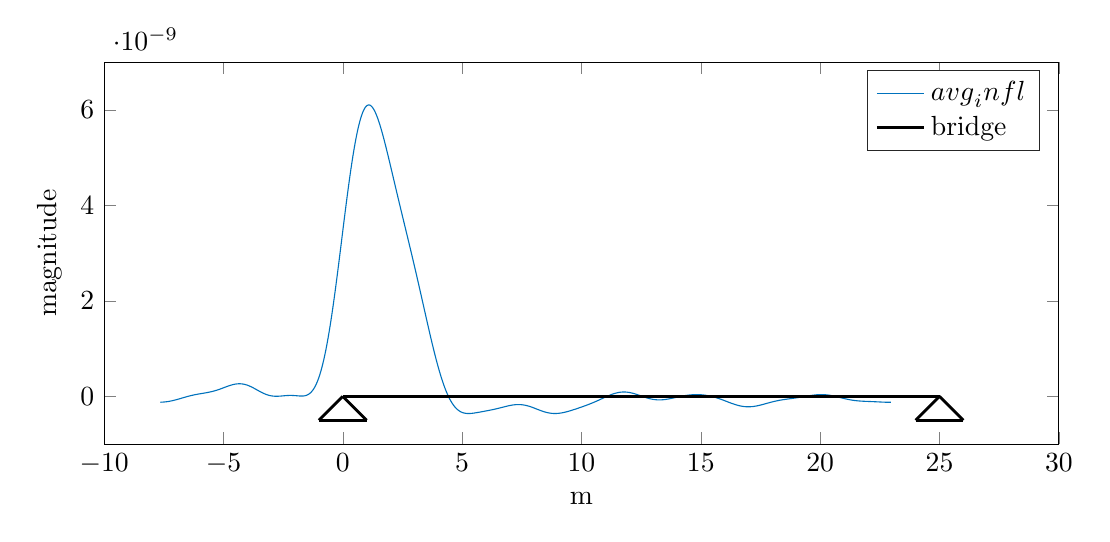
\begin{tikzpicture}

  \begin{axis}[%
    width=\textwidth,
    height=0.4\textwidth,
    at={(0\figurewidth,0\figureheight)},
    scale only axis,
    xmin=-10,
    xmax=30,
    xlabel={m},
    ymin=-1e-09,
    ymax=7e-09,
    ylabel={magnitude},
    axis background/.style={fill=white},
    title style={font=\bfseries},
    title={},
    legend style={legend cell align=left,align=left,draw=white!15!black}
    ]
    \addplot [color=mycolor1,solid]
    table[row sep=crcr]{%
    -7.64224200195312	-1.23184355852725e-10\\
    -7.62213314941406	-1.22819037602068e-10\\
    -7.602024296875	-1.22384658510883e-10\\
    -7.58191544433594	-1.21879184811863e-10\\
    -7.56180659179687	-1.21300723199635e-10\\
    -7.54169773925781	-1.20647529719041e-10\\
    -7.52158888671875	-1.19918018147e-10\\
    -7.50148003417969	-1.1911076783271e-10\\
    -7.48137118164062	-1.18224530962781e-10\\
    -7.46126232910156	-1.17258239219868e-10\\
    -7.4411534765625	-1.16211009805576e-10\\
    -7.42104462402344	-1.15082150800468e-10\\
    -7.40093577148437	-1.13871165836554e-10\\
    -7.38082691894531	-1.12577758059947e-10\\
    -7.36071806640625	-1.11201833363985e-10\\
    -7.34060921386719	-1.09743502875708e-10\\
    -7.32050036132812	-1.08203084681361e-10\\
    -7.30039150878906	-1.0658110477931e-10\\
    -7.28028265625	-1.04878297251598e-10\\
    -7.26017380371094	-1.03095603648326e-10\\
    -7.24006495117187	-1.01234171581895e-10\\
    -7.21995609863281	-9.92953525311304e-11\\
    -7.19984724609375	-9.72806988583129e-11\\
    -7.17973839355469	-9.51919600450536e-11\\
    -7.15962954101562	-9.30310781559983e-11\\
    -7.13952068847656	-9.08001825422562e-11\\
    -7.1194118359375	-8.85015837994248e-11\\
    -7.09930298339844	-8.61377669979372e-11\\
    -7.07919413085937	-8.37113842063614e-11\\
    -7.05908527832031	-8.12252463310308e-11\\
    -7.03897642578125	-7.86823142981376e-11\\
    -7.01886757324219	-7.60856896070786e-11\\
    -6.99875872070312	-7.34386042863496e-11\\
    -6.97864986816406	-7.07444102858321e-11\\
    -6.958541015625	-6.80065683415596e-11\\
    -6.93843216308594	-6.52286363513978e-11\\
    -6.91832331054687	-6.24142573021078e-11\\
    -6.89821445800781	-5.95671467902204e-11\\
    -6.87810560546875	-5.66910801811071e-11\\
    -6.85799675292969	-5.37898794521273e-11\\
    -6.83788790039062	-5.08673997674125e-11\\
    -6.81777904785156	-4.7927515833143e-11\\
    -6.7976701953125	-4.49741080833632e-11\\
    -6.77756134277344	-4.20110487473899e-11\\
    -6.75745249023437	-3.904218785077e-11\\
    -6.73734363769531	-3.60713392022806e-11\\
    -6.71723478515625	-3.31022664200428e-11\\
    -6.69712593261719	-3.01386690500205e-11\\
    -6.67701708007812	-2.71841688302832e-11\\
    -6.65690822753906	-2.42422961542935e-11\\
    -6.636799375	-2.1316476786168e-11\\
    -6.61669052246094	-1.84100188803513e-11\\
    -6.59658166992187	-1.5526100357454e-11\\
    -6.57647281738281	-1.26677566871027e-11\\
    -6.55636396484375	-9.83786912752608e-12\\
    -6.53625511230469	-7.0391534704213e-12\\
    -6.51614625976562	-4.27414933805455e-12\\
    -6.49603740722656	-1.54521007799983e-12\\
    -6.4759285546875	1.14550670094651e-12\\
    -6.45581970214844	3.79604791012802e-12\\
    -6.43571084960937	6.40467304030847e-12\\
    -6.41560199707031	8.96986146175817e-12\\
    -6.39549314453125	1.14903189306391e-11\\
    -6.37538429199219	1.39649832696723e-11\\
    -6.35527543945312	1.63930291939307e-11\\
    -6.33516658691406	1.87738722554385e-11\\
    -6.315057734375	2.11071718832793e-11\\
    -6.29494888183594	2.33928334990348e-11\\
    -6.27484002929687	2.56310096906044e-11\\
    -6.25473117675781	2.78221004307024e-11\\
    -6.23462232421875	2.99667523298182e-11\\
    -6.21451347167969	3.2065856916746e-11\\
    -6.19440461914062	3.41205479433811e-11\\
    -6.17429576660156	3.61321977139952e-11\\
    -6.1541869140625	3.81024124427487e-11\\
    -6.13407806152344	4.00330266468303e-11\\
    -6.11396920898437	4.19260965861701e-11\\
    -6.09386035644531	4.37838927642691e-11\\
    -6.07375150390625	4.56088915082676e-11\\
    -6.05364265136719	4.74037656498709e-11\\
    -6.03353379882812	4.91713743322486e-11\\
    -6.01342494628906	5.09147519714726e-11\\
    -5.99331609375	5.26370964043541e-11\\
    -5.97320724121094	5.4341756257847e-11\\
    -5.95309838867187	5.60322175783496e-11\\
    -5.93298953613281	5.77120897622951e-11\\
    -5.91288068359375	5.93850908323249e-11\\
    -5.89277183105469	6.10550321062299e-11\\
    -5.87266297851562	6.27258023084164e-11\\
    -5.85255412597656	6.44013511762326e-11\\
    -5.8324452734375	6.60856726158204e-11\\
    -5.81233642089844	6.77827874643097e-11\\
    -5.79222756835937	6.94967259172181e-11\\
    -5.77211871582031	7.12315096816741e-11\\
    -5.75200986328125	7.29911339176921e-11\\
    -5.73190101074219	7.47795490311852e-11\\
    -5.71179215820312	7.66006423834899e-11\\
    -5.69168330566406	7.84582199832417e-11\\
    -5.671574453125	8.03559882271075e-11\\
    -5.65146560058594	8.22975357564815e-11\\
    -5.63135674804687	8.42863154974262e-11\\
    -5.61124789550781	8.63256269513034e-11\\
    -5.59113904296875	8.84185988032808e-11\\
    -5.57103019042969	9.05681719154974e-11\\
    -5.55092133789062	9.27770827710187e-11\\
    -5.53081248535156	9.50478474337724e-11\\
    -5.5107036328125	9.73827460885796e-11\\
    -5.49059478027344	9.97838082239474e-11\\
    -5.47048592773437	1.0225279851873e-10\\
    -5.45037707519531	1.0479120349194e-10\\
    -5.43026822265625	1.07400218972846e-10\\
    -5.41015937011719	1.1008073844633e-10\\
    -5.39005051757812	1.1283334232589e-10\\
    -5.36994166503906	1.1565828820399e-10\\
    -5.3498328125	1.18555502126614e-10\\
    -5.32972395996094	1.21524570935702e-10\\
    -5.30961510742187	1.24564735719933e-10\\
    -5.28950625488281	1.27674886410862e-10\\
    -5.26939740234375	1.30853557557773e-10\\
    -5.24928854980469	1.34098925310922e-10\\
    -5.22917969726562	1.37408805638857e-10\\
    -5.20907084472656	1.4078065380156e-10\\
    -5.1889619921875	1.44211565096958e-10\\
    -5.16885313964844	1.4769827689412e-10\\
    -5.14874428710937	1.51237171962173e-10\\
    -5.12863543457031	1.54824283099494e-10\\
    -5.10852658203125	1.58455299063334e-10\\
    -5.08841772949219	1.62125571795523e-10\\
    -5.06830887695312	1.6583012493529e-10\\
    -5.04820002441406	1.69563663605846e-10\\
    -5.028091171875	1.73320585456643e-10\\
    -5.00798231933594	1.77094992938854e-10\\
    -4.98787346679687	1.80880706787016e-10\\
    -4.96776461425781	1.84671280675409e-10\\
    -4.94765576171875	1.88460017013282e-10\\
    -4.92754690917969	1.92239983838841e-10\\
    -4.90743805664062	1.96004032767578e-10\\
    -4.88732920410156	1.99744817946548e-10\\
    -4.8672203515625	2.03454815962147e-10\\
    -4.84711149902344	2.07126346645143e-10\\
    -4.82700264648437	2.10751594713042e-10\\
    -4.80689379394531	2.14322632186344e-10\\
    -4.78678494140625	2.17831441511929e-10\\
    -4.76667608886719	2.21269939323704e-10\\
    -4.74656723632812	2.2463000076764e-10\\
    -4.72645838378906	2.27903484315743e-10\\
    -4.70634953125	2.31082256990903e-10\\
    -4.68624067871094	2.3415821992245e-10\\
    -4.66613182617187	2.37123334150107e-10\\
    -4.64602297363281	2.39969646592521e-10\\
    -4.62591412109375	2.42689316094868e-10\\
    -4.60580526855469	2.4527463946901e-10\\
    -4.58569641601562	2.47718077438714e-10\\
    -4.56558756347656	2.50012280401821e-10\\
    -4.5454787109375	2.52150113920995e-10\\
    -4.52536985839844	2.54124683854559e-10\\
    -4.50526100585937	2.55929361039316e-10\\
    -4.48515215332031	2.57557805437713e-10\\
    -4.46504330078125	2.59003989662692e-10\\
    -4.44493444824219	2.60262221794641e-10\\
    -4.42482559570312	2.61327167406437e-10\\
    -4.40471674316406	2.6219387071429e-10\\
    -4.384607890625	2.62857774774181e-10\\
    -4.36449903808594	2.63314740646046e-10\\
    -4.34439018554687	2.63561065450563e-10\\
    -4.32428133300781	2.63593499246204e-10\\
    -4.30417248046875	2.63409260657582e-10\\
    -4.28406362792969	2.63006051189425e-10\\
    -4.26395477539062	2.62382068164366e-10\\
    -4.24384592285156	2.61536016226623e-10\\
    -4.2237370703125	2.60467117357862e-10\\
    -4.20362821777344	2.59175119356013e-10\\
    -4.18351936523437	2.57660302732355e-10\\
    -4.16341051269531	2.55923485987127e-10\\
    -4.14330166015625	2.53966029228843e-10\\
    -4.12319280761719	2.51789836107728e-10\\
    -4.10308395507812	2.49397354039027e-10\\
    -4.08297510253906	2.46791572697419e-10\\
    -4.06286625	2.43976020769309e-10\\
    -4.04275739746094	2.40954760955565e-10\\
    -4.02264854492188	2.37732383222946e-10\\
    -4.00253969238281	2.34313996308418e-10\\
    -3.98243083984375	2.30705217486351e-10\\
    -3.96232198730469	2.26912160614601e-10\\
    -3.94221313476562	2.22941422481362e-10\\
    -3.92210428222656	2.18800067480622e-10\\
    -3.9019954296875	2.14495610649965e-10\\
    -3.88188657714844	2.10035999110276e-10\\
    -3.86177772460937	2.05429591952716e-10\\
    -3.84166887207031	2.00685138624011e-10\\
    -3.82156001953125	1.95811755866679e-10\\
    -3.80145116699219	1.9081890327632e-10\\
    -3.78134231445312	1.85716357543313e-10\\
    -3.76123346191406	1.80514185451528e-10\\
    -3.741124609375	1.7522271571152e-10\\
    -3.72101575683594	1.69852509710517e-10\\
    -3.70090690429687	1.64414331265994e-10\\
    -3.68079805175781	1.58919115473993e-10\\
    -3.66068919921875	1.53377936747338e-10\\
    -3.64058034667969	1.47801976142776e-10\\
    -3.62047149414062	1.42202488079484e-10\\
    -3.60036264160156	1.36590766554667e-10\\
    -3.5802537890625	1.30978110964832e-10\\
    -3.56014493652344	1.25375791643949e-10\\
    -3.54003608398437	1.19795015231867e-10\\
    -3.51992723144531	1.14246889988379e-10\\
    -3.49981837890625	1.08742391169773e-10\\
    -3.47970952636719	1.03292326585917e-10\\
    -3.45960067382812	9.79073024567982e-11\\
    -3.43949182128906	9.25976896877902e-11\\
    -3.41938296875	8.73735906830372e-11\\
    -3.39927411621094	8.22448068159942e-11\\
    -3.37916526367187	7.72208066754529e-11\\
    -3.35905641113281	7.23106952042851e-11\\
    -3.33894755859375	6.75231838466056e-11\\
    -3.31883870605469	6.28665618172133e-11\\
    -3.29872985351562	5.83486686048882e-11\\
    -3.27862100097656	5.39768678184067e-11\\
    -3.2585121484375	4.97580224812321e-11\\
    -3.23840329589844	4.56984718772442e-11\\
    -3.21829444335937	4.18040100462933e-11\\
    -3.19818559082031	3.80798660240592e-11\\
    -3.17807673828125	3.45306859163312e-11\\
    -3.15796788574219	3.11605168929363e-11\\
    -3.13785903320312	2.79727931814226e-11\\
    -3.11775018066406	2.49703241351391e-11\\
    -3.097641328125	2.21552844445968e-11\\
    -3.07753247558594	1.95292065549319e-11\\
    -3.05742362304687	1.70929753459981e-11\\
    -3.03731477050781	1.48468251250627e-11\\
    -3.01720591796875	1.27903389752407e-11\\
    -2.99709706542969	1.09224504958238e-11\\
    -2.97698821289062	9.24144796345566e-12\\
    -2.95687936035156	7.74498093571828e-12\\
    -2.9367705078125	6.43006931113168e-12\\
    -2.91666165527344	5.29311485198541e-12\\
    -2.89655280273437	4.32991516854061e-12\\
    -2.87644395019531	3.53568015539713e-12\\
    -2.85633509765625	2.9050508628059e-12\\
    -2.83622624511719	2.43212077781919e-12\\
    -2.81611739257812	2.11045948216203e-12\\
    -2.79600854003906	1.93313864576743e-12\\
    -2.7758996875	1.89276030699762e-12\\
    -2.75579083496094	1.9814873826808e-12\\
    -2.73568198242187	2.19107634337418e-12\\
    -2.71557312988281	2.5129119815178e-12\\
    -2.69546427734375	2.93804419269107e-12\\
    -2.67535542480469	3.45722668273349e-12\\
    -2.65524657226562	4.0609575063618e-12\\
    -2.63513771972656	4.73952133589756e-12\\
    -2.6150288671875	5.48303335195141e-12\\
    -2.59492001464844	6.28148464144415e-12\\
    -2.57481116210937	7.12478898209249e-12\\
    -2.55470230957031	8.00283088655542e-12\\
    -2.53459345703125	8.90551477382799e-12\\
    -2.51448460449219	9.82281513020578e-12\\
    -2.49437575195312	1.0744827517188e-11\\
    -2.47426689941406	1.16618202791839e-11\\
    -2.454158046875	1.25642867997092e-11\\
    -2.43404919433594	1.34429981510127e-11\\
    -2.41394034179687	1.42890559787751e-11\\
    -2.39383148925781	1.50939454606275e-11\\
    -2.37372263671875	1.58495881747686e-11\\
    -2.35361378417969	1.65483947130865e-11\\
    -2.33350493164062	1.71833168715584e-11\\
    -2.31339607910156	1.77478992498406e-11\\
    -2.2932872265625	1.82363300912548e-11\\
    -2.27317837402344	1.86434911945286e-11\\
    -2.25306952148437	1.89650067289725e-11\\
    -2.23296066894531	1.91972907858239e-11\\
    -2.21285181640625	1.93375934999168e-11\\
    -2.19274296386719	1.93840455778706e-11\\
    -2.17263411132812	1.93357010714008e-11\\
    -2.15252525878906	1.91925782374121e-11\\
    -2.13241640625	1.89556983299654e-11\\
    -2.11230755371094	1.862712217319e-11\\
    -2.09219870117187	1.82099843686938e-11\\
    -2.07208984863281	1.77085249959164e-11\\
    -2.05198099609375	1.71281186693059e-11\\
    -2.03187214355469	1.6475300821988e-11\\
    -2.01176329101562	1.57577910919635e-11\\
    -1.99165443847656	1.49845136935157e-11\\
    -1.9715455859375	1.41656146636488e-11\\
    -1.95143673339844	1.33124758809294e-11\\
    -1.93132788085937	1.24377257619226e-11\\
    -1.91121902832031	1.15552465487404e-11\\
    -1.89111017578125	1.0680178109714e-11\\
    -1.87100132324219	9.82891818414528e-12\\
    -1.85089247070312	9.01911901124407e-12\\
    -1.83078361816406	8.2696802928143e-12\\
    -1.810674765625	7.60073844888787e-12\\
    -1.79056591308594	7.03365213546064e-12\\
    -1.77045706054687	6.59098400350577e-12\\
    -1.75034820800781	6.29647868870075e-12\\
    -1.73023935546875	6.17503703169125e-12\\
    -1.71013050292969	6.25268653912152e-12\\
    -1.69002165039062	6.55654810628746e-12\\
    -1.66991279785156	7.11479903278858e-12\\
    -1.6498039453125	7.9566323731702e-12\\
    -1.62969509277344	9.11221267516816e-12\\
    -1.60958624023437	1.06126281686391e-11\\
    -1.58947738769531	1.24898394787677e-11\\
    -1.56936853515625	1.47766249474864e-11\\
    -1.54925968261719	1.75065226572286e-11\\
    -1.52915083007812	2.07137692612183e-11\\
    -1.50904197753906	2.4433235734314e-11\\
    -1.488933125	2.87003601680785e-11\\
    -1.46882427246094	3.35510777430786e-11\\
    -1.44871541992187	3.90217480205239e-11\\
    -1.42860656738281	4.5149079704128e-11\\
    -1.40849771484375	5.19700530314635e-11\\
    -1.38838886230469	5.95218399622195e-11\\
    -1.36828000976562	6.7841722338363e-11\\
    -1.34817115722656	7.69670081985677e-11\\
    -1.3280623046875	8.69349464359799e-11\\
    -1.30795345214844	9.77826399948757e-11\\
    -1.28784459960937	1.09546957807558e-10\\
    -1.26773574707031	1.22264445678275e-10\\
    -1.24762689453125	1.3597123632578e-10\\
    -1.22751804199219	1.5070295880053e-10\\
    -1.20740918945312	1.66494647496224e-10\\
    -1.18730033691406	1.83380650978669e-10\\
    -1.167191484375	2.01394540857548e-10\\
    -1.14708263183594	2.20569020928762e-10\\
    -1.12697377929687	2.40935836816399e-10\\
    -1.10686492675781	2.6252568634429e-10\\
    -1.08675607421875	2.85368130867325e-10\\
    -1.06664722167969	3.09491507792292e-10\\
    -1.04653836914062	3.34922844517031e-10\\
    -1.02642951660156	3.61687774015065e-10\\
    -1.0063206640625	3.89810452290608e-10\\
    -0.986211811523437	4.19313477926045e-10\\
    -0.966102958984375	4.50217813940411e-10\\
    -0.945994106445312	4.82542712173454e-10\\
    -0.92588525390625	5.1630564040506e-10\\
    -0.905776401367187	5.51522212414655e-10\\
    -0.885667548828125	5.88206121179321e-10\\
    -0.865558696289062	6.26369075402933e-10\\
    -0.845449843749999	6.66020739561729e-10\\
    -0.825340991210937	7.07168677644198e-10\\
    -0.805232138671874	7.49818300755184e-10\\
    -0.785123286132812	7.9397281874558e-10\\
    -0.765014433593749	8.39633196020071e-10\\
    -0.744905581054687	8.86798111665881e-10\\
    -0.724796728515624	9.35463924035677e-10\\
    -0.704687875976562	9.85624639907491e-10\\
    -0.684579023437499	1.03727188833391e-09\\
    -0.664470170898437	1.09039489928171e-09\\
    -0.644361318359374	1.14498048715194e-09\\
    -0.624252465820312	1.20101303925865e-09\\
    -0.604143613281249	1.25847450933277e-09\\
    -0.584034760742187	1.3173444161054e-09\\
    -0.563925908203124	1.37759984701256e-09\\
    -0.543817055664062	1.43921546705084e-09\\
    -0.523708203125	1.50216353280094e-09\\
    -0.503599350585937	1.56641391162323e-09\\
    -0.483490498046875	1.63193410601675e-09\\
    -0.463381645507812	1.69868928312018e-09\\
    -0.44327279296875	1.76664230932057e-09\\
    -0.423163940429687	1.83575378992286e-09\\
    -0.403055087890625	1.90598211382024e-09\\
    -0.382946235351562	1.97728350309327e-09\\
    -0.3628373828125	2.04961206745263e-09\\
    -0.342728530273437	2.12291986342863e-09\\
    -0.322619677734375	2.19715695819802e-09\\
    -0.302510825195312	2.27227149792721e-09\\
    -0.28240197265625	2.34820978049904e-09\\
    -0.262293120117187	2.42491633247933e-09\\
    -0.242184267578124	2.50233399016816e-09\\
    -0.222075415039062	2.58040398457045e-09\\
    -0.201966562499999	2.65906603011024e-09\\
    -0.181857709960937	2.73825841690314e-09\\
    -0.161748857421874	2.81791810639226e-09\\
    -0.141640004882812	2.89798083014403e-09\\
    -0.121531152343749	2.97838119159201e-09\\
    -0.101422299804687	3.05905277050891e-09\\
    -0.0813134472656243	3.13992822997991e-09\\
    -0.0612045947265623	3.22093942564351e-09\\
    -0.0410957421874993	3.3020175169601e-09\\
    -0.0209868896484373	3.38309308026309e-09\\
    -0.000878037109374397	3.46409622334214e-09\\
    0.0192308154296876	3.5449567013043e-09\\
    0.0393396679687505	3.62560403345473e-09\\
    0.0594485205078126	3.70596762093626e-09\\
    0.0795573730468755	3.78597686486422e-09\\
    0.0996662255859384	3.86556128469179e-09\\
    0.119775078125	3.94465063653993e-09\\
    0.139883930664063	4.02317503122583e-09\\
    0.159992783203125	4.10106505172408e-09\\
    0.180101635742188	4.17825186979615e-09\\
    0.20021048828125	4.25466736152522e-09\\
    0.220319340820313	4.33024422149616e-09\\
    0.240428193359375	4.40491607536338e-09\\
    0.260537045898438	4.47861759055321e-09\\
    0.2806458984375	4.55128458485183e-09\\
    0.300754750976563	4.62285413263498e-09\\
    0.320863603515625	4.69326466850113e-09\\
    0.340972456054688	4.76245608807653e-09\\
    0.361081308593751	4.83036984576707e-09\\
    0.381190161132813	4.8969490492397e-09\\
    0.401299013671875	4.962138550424e-09\\
    0.421407866210939	5.02588503283326e-09\\
    0.441516718750001	5.08813709501337e-09\\
    0.461625571289063	5.14884532993765e-09\\
    0.481734423828125	5.20796240017552e-09\\
    0.501843276367189	5.26544310867361e-09\\
    0.521952128906251	5.32124446499885e-09\\
    0.542060981445313	5.37532574690418e-09\\
    0.562169833984375	5.42764855708928e-09\\
    0.582278686523439	5.4781768750407e-09\\
    0.602387539062501	5.52687710384785e-09\\
    0.622496391601563	5.57371811190397e-09\\
    0.642605244140625	5.61867126941391e-09\\
    0.662714096679689	5.66171047964306e-09\\
    0.682822949218751	5.70281220485554e-09\\
    0.702931801757813	5.74195548690213e-09\\
    0.723040654296875	5.77912196243214e-09\\
    0.743149506835938	5.81429587271657e-09\\
    0.763258359375	5.84746406808317e-09\\
    0.783367211914062	5.87861600697726e-09\\
    0.803476064453126	5.90774374967534e-09\\
    0.823584916992188	5.93484194669174e-09\\
    0.84369376953125	5.95990782193139e-09\\
    0.863802622070312	5.98294115065453e-09\\
    0.883911474609376	6.00394423233206e-09\\
    0.904020327148438	6.02292185848211e-09\\
    0.9241291796875	6.03988127559103e-09\\
    0.944238032226562	6.05483214323334e-09\\
    0.964346884765626	6.06778648751686e-09\\
    0.984455737304688	6.0787586499903e-09\\
    1.00456458984375	6.08776523216122e-09\\
    1.02467344238281	6.09482503578265e-09\\
    1.04478229492188	6.09995899907638e-09\\
    1.06489114746094	6.10319012907038e-09\\
    1.085	6.10454343023671e-09\\
    1.10510885253906	6.10404582962442e-09\\
    1.12521770507813	6.10172609869004e-09\\
    1.14532655761719	6.09761477203535e-09\\
    1.16543541015625	6.0917440632687e-09\\
    1.18554426269531	6.08414777821251e-09\\
    1.20565311523438	6.07486122568479e-09\\
    1.22576196777344	6.0639211260875e-09\\
    1.2458708203125	6.05136551803875e-09\\
    1.26597967285156	6.03723366328947e-09\\
    1.28608852539063	6.02156595016798e-09\\
    1.30619737792969	6.00440379579839e-09\\
    1.32630623046875	5.98578954734011e-09\\
    1.34641508300781	5.96576638249686e-09\\
    1.36652393554688	5.94437820954388e-09\\
    1.38663278808594	5.92166956712158e-09\\
    1.406741640625	5.89768552404281e-09\\
    1.42685049316406	5.87247157935948e-09\\
    1.44695934570313	5.84607356293158e-09\\
    1.46706819824219	5.81853753673913e-09\\
    1.48717705078125	5.78990969717345e-09\\
    1.50728590332031	5.76023627854055e-09\\
    1.52739475585938	5.72956345800418e-09\\
    1.54750360839844	5.6979372621909e-09\\
    1.5676124609375	5.66540347567351e-09\\
    1.58772131347656	5.63200755154285e-09\\
    1.60783016601563	5.59779452427065e-09\\
    1.62793901855469	5.56280892505886e-09\\
    1.64804787109375	5.52709469986283e-09\\
    1.66815672363281	5.490695130267e-09\\
    1.68826557617188	5.45365275738323e-09\\
    1.70837442871094	5.41600930893233e-09\\
    1.72848328125	5.37780562965969e-09\\
    1.74859213378906	5.3390816152259e-09\\
    1.76870098632812	5.29987614970304e-09\\
    1.78880983886719	5.26022704679628e-09\\
    1.80891869140625	5.2201709949e-09\\
    1.82902754394531	5.17974350608599e-09\\
    1.84913639648437	5.13897886911054e-09\\
    1.86924524902344	5.09791010651505e-09\\
    1.8893541015625	5.05656893588374e-09\\
    1.90946295410156	5.01498573531002e-09\\
    1.92957180664062	4.97318951311121e-09\\
    1.94968065917969	4.93120788181986e-09\\
    1.96978951171875	4.8890670364675e-09\\
    1.98989836425781	4.84679173716542e-09\\
    2.01000721679688	4.80440529597506e-09\\
    2.03011606933594	4.76192956804894e-09\\
    2.050224921875	4.71938494701178e-09\\
    2.07033377441406	4.67679036453987e-09\\
    2.09044262695313	4.63416329408581e-09\\
    2.11055147949219	4.59151975868481e-09\\
    2.13066033203125	4.54887434276789e-09\\
    2.15076918457031	4.50624020789721e-09\\
    2.17087803710938	4.46362911232855e-09\\
    2.19098688964844	4.42105143429621e-09\\
    2.2110957421875	4.3785161989064e-09\\
    2.23120459472656	4.33603110851591e-09\\
    2.25131344726563	4.29360257646463e-09\\
    2.27142229980469	4.25123576402219e-09\\
    2.29153115234375	4.20893462040118e-09\\
    2.31164000488281	4.16670192568245e-09\\
    2.33174885742188	4.12453933649112e-09\\
    2.35185770996094	4.08244743425572e-09\\
    2.3719665625	4.0404257758772e-09\\
    2.39207541503906	3.99847294662942e-09\\
    2.41218426757813	3.95658661510809e-09\\
    2.43229312011719	3.91476359004095e-09\\
    2.45240197265625	3.87299987876875e-09\\
    2.47251082519531	3.83129074720332e-09\\
    2.49261967773438	3.78963078106697e-09\\
    2.51272853027344	3.74801394821544e-09\\
    2.5328373828125	3.70643366184548e-09\\
    2.55294623535156	3.66488284438774e-09\\
    2.57305508789063	3.62335399188511e-09\\
    2.59316394042969	3.58183923865767e-09\\
    2.61327279296875	3.54033042205625e-09\\
    2.63338164550781	3.49881914710824e-09\\
    2.65349049804688	3.45729685086154e-09\\
    2.67359935058594	3.41575486623535e-09\\
    2.693708203125	3.37418448518962e-09\\
    2.71381705566406	3.33257702102892e-09\\
    2.73392590820313	3.29092386966065e-09\\
    2.75403476074219	3.24921656963244e-09\\
    2.77414361328125	3.20744686077863e-09\\
    2.79425246582031	3.16560674131173e-09\\
    2.81436131835938	3.12368852320049e-09\\
    2.83447017089844	3.08168488568319e-09\\
    2.8545790234375	3.03958892677124e-09\\
    2.87468787597656	2.99739421260598e-09\\
    2.89479672851563	2.95509482453869e-09\\
    2.91490558105469	2.91268540381224e-09\\
    2.93501443359375	2.87016119373062e-09\\
    2.95512328613281	2.82751807921166e-09\\
    2.97523213867188	2.7847526236263e-09\\
    2.99534099121094	2.74186210283745e-09\\
    3.01544984375	2.69884453636008e-09\\
    3.03555869628906	2.65569871557379e-09\\
    3.05566754882812	2.61242422892845e-09\\
    3.07577640136719	2.56902148409308e-09\\
    3.09588525390625	2.52549172700745e-09\\
    3.11599410644531	2.48183705780621e-09\\
    3.13610295898437	2.43806044359407e-09\\
    3.15621181152344	2.39416572806107e-09\\
    3.1763206640625	2.35015763793595e-09\\
    3.19642951660156	2.30604178628547e-09\\
    3.21653836914062	2.26182467267683e-09\\
    3.23664722167969	2.21751368022972e-09\\
    3.25675607421875	2.17311706959338e-09\\
    3.27686492675781	2.12864396989358e-09\\
    3.29697377929687	2.08410436670237e-09\\
    3.31708263183594	2.03950908709283e-09\\
    3.337191484375	1.99486978184857e-09\\
    3.35730033691406	1.95019890490621e-09\\
    3.37740918945313	1.9055096901165e-09\\
    3.39751804199219	1.86081612541721e-09\\
    3.41762689453125	1.81613292451788e-09\\
    3.43773574707031	1.77147549620335e-09\\
    3.45784459960938	1.72685991136891e-09\\
    3.47795345214844	1.68230286790636e-09\\
    3.4980623046875	1.63782165356524e-09\\
    3.51817115722656	1.59343410691885e-09\\
    3.53828000976563	1.54915857656939e-09\\
    3.55838886230469	1.50501387873042e-09\\
    3.57849771484375	1.46101925332897e-09\\
    3.59860656738281	1.41719431877268e-09\\
    3.61871541992188	1.37355902553026e-09\\
    3.63882427246094	1.33013360867589e-09\\
    3.658933125	1.28693853955014e-09\\
    3.67904197753906	1.24399447669124e-09\\
    3.69915083007813	1.20132221619158e-09\\
    3.71925968261719	1.15894264163477e-09\\
    3.73936853515625	1.11687667376852e-09\\
    3.75947738769531	1.07514522006806e-09\\
    3.77958624023438	1.03376912434405e-09\\
    3.79969509277344	9.92769116547206e-10\\
    3.8198039453125	9.52165762920419e-10\\
    3.83991279785156	9.11979416646352e-10\\
    3.86002165039063	8.72230169136167e-10\\
    3.88013050292969	8.32937802101671e-10\\
    3.90023935546875	7.94121740549603e-10\\
    3.92034820800781	7.55801006832941e-10\\
    3.94045706054688	7.17994175889623e-10\\
    3.96056591308594	6.80719331794514e-10\\
    3.980674765625	6.43994025745297e-10\\
    4.00078361816406	6.07835235597718e-10\\
    4.02089247070313	5.72259327059786e-10\\
    4.04100132324219	5.37282016648738e-10\\
    4.06111017578125	5.02918336508227e-10\\
    4.08121902832031	4.69182601176752e-10\\
    4.10132788085938	4.36088376391693e-10\\
    4.12143673339844	4.03648450006357e-10\\
    4.1415455859375	3.71874805090397e-10\\
    4.16165443847656	3.40778595276736e-10\\
    4.18176329101563	3.10370122410748e-10\\
    4.20187214355469	2.80658816549987e-10\\
    4.22198099609375	2.51653218355216e-10\\
    4.24208984863281	2.23360963905816e-10\\
    4.26219870117187	1.957887719651e-10\\
    4.28230755371094	1.6894243371328e-10\\
    4.30241640625	1.4282680495828e-10\\
    4.32252525878906	1.17445800826922e-10\\
    4.34263411132812	9.28023929314456e-11\\
    4.36274296386719	6.88986089988939e-11\\
    4.38285181640625	4.57355349434656e-11\\
    4.40296066894531	2.33133193547434e-11\\
    4.42306952148437	1.63118036756825e-12\\
    4.44317837402344	-1.93125851275896e-11\\
    4.4632872265625	-3.95205899816317e-11\\
    4.48339607910156	-5.89963430456479e-11\\
    4.50350493164062	-7.77442332522573e-11\\
    4.52361378417969	-9.57695115862664e-11\\
    4.54372263671875	-1.13078271017263e-10\\
    4.56383148925781	-1.29677424472199e-10\\
    4.58394034179688	-1.45574680931389e-10\\
    4.60404919433594	-1.60778519736113e-10\\
    4.624158046875	-1.7529816320077e-10\\
    4.64426689941406	-1.89143547626674e-10\\
    4.66437575195313	-2.02325292818632e-10\\
    4.68448460449219	-2.14854670208903e-10\\
    4.70459345703125	-2.26743569696501e-10\\
    4.72470230957031	-2.38004465312522e-10\\
    4.74481116210938	-2.4865037982475e-10\\
    4.76492001464844	-2.58694848396874e-10\\
    4.7850288671875	-2.68151881419366e-10\\
    4.80513771972656	-2.77035926630427e-10\\
    4.82524657226563	-2.8536183064634e-10\\
    4.84535542480469	-2.93144800021196e-10\\
    4.86546427734375	-3.00400361956081e-10\\
    4.88557312988281	-3.07144324777685e-10\\
    4.90568198242188	-3.13392738305701e-10\\
    4.92579083496094	-3.1916185422744e-10\\
    4.9458996875	-3.24468086596819e-10\\
    4.96600854003906	-3.293279725732e-10\\
    4.98611739257813	-3.33758133513546e-10\\
    5.00622624511719	-3.37775236529037e-10\\
    5.02633509765625	-3.41395956614597e-10\\
    5.04644395019531	-3.44636939456783e-10\\
    5.06655280273438	-3.47514765022212e-10\\
    5.08666165527344	-3.50045912025083e-10\\
    5.1067705078125	-3.52246723368491e-10\\
    5.12687936035156	-3.54133372650097e-10\\
    5.14698821289063	-3.55721831818325e-10\\
    5.16709706542969	-3.57027840060648e-10\\
    5.18720591796875	-3.58066874000686e-10\\
    5.20731477050781	-3.58854119275823e-10\\
    5.22742362304688	-3.59404443561799e-10\\
    5.24753247558594	-3.59732371105439e-10\\
    5.267641328125	-3.59852058821046e-10\\
    5.28775018066406	-3.59777274000488e-10\\
    5.30785903320313	-3.59521373681121e-10\\
    5.32796788574219	-3.59097285709967e-10\\
    5.34807673828125	-3.58517491536611e-10\\
    5.36818559082031	-3.57794010761356e-10\\
    5.38829444335938	-3.56938387459185e-10\\
    5.40840329589844	-3.5596167829415e-10\\
    5.4285121484375	-3.54874442432778e-10\\
    5.44862100097656	-3.53686733259175e-10\\
    5.46872985351563	-3.52408091888682e-10\\
    5.48883870605469	-3.51047542470986e-10\\
    5.50894755859375	-3.49613589268039e-10\\
    5.52905641113281	-3.4811421548636e-10\\
    5.54916526367187	-3.4655688383787e-10\\
    5.56927411621094	-3.44948538798068e-10\\
    5.58938296875	-3.43295610525106e-10\\
    5.60949182128906	-3.41604020398314e-10\\
    5.62960067382812	-3.39879188129875e-10\\
    5.64970952636719	-3.38126040398724e-10\\
    5.66981837890625	-3.36349020951291e-10\\
    5.68992723144531	-3.34552102109507e-10\\
    5.71003608398437	-3.32738797622574e-10\\
    5.73014493652344	-3.30912176795228e-10\\
    5.7502537890625	-3.29074879821797e-10\\
    5.77036264160156	-3.27229134252204e-10\\
    5.79047149414062	-3.25376772513084e-10\\
    5.81058034667969	-3.23519250404663e-10\\
    5.83068919921875	-3.21657666491623e-10\\
    5.85079805175781	-3.19792782304211e-10\\
    5.87090690429687	-3.17925043264082e-10\\
    5.89101575683594	-3.16054600247949e-10\\
    5.911124609375	-3.14181331700987e-10\\
    5.93123346191406	-3.12304866211138e-10\\
    5.95134231445313	-3.10424605454902e-10\\
    5.97145116699219	-3.08539747425088e-10\\
    5.99156001953125	-3.06649309851e-10\\
    6.01166887207031	-3.04752153722e-10\\
    6.03177772460938	-3.02847006826082e-10\\
    6.05188657714844	-3.00932487216056e-10\\
    6.0719954296875	-2.99007126517261e-10\\
    6.09210428222656	-2.97069392992233e-10\\
    6.11221313476563	-2.95117714279656e-10\\
    6.13232198730469	-2.93150499726961e-10\\
    6.15243083984375	-2.91166162238316e-10\\
    6.17253969238281	-2.89163139562348e-10\\
    6.19264854492188	-2.87139914946784e-10\\
    6.21275739746094	-2.85095037090189e-10\\
    6.23286625	-2.83027139324351e-10\\
    6.25297510253906	-2.80934957964222e-10\\
    6.27308395507813	-2.78817349766044e-10\\
    6.29319280761719	-2.7667330843807e-10\\
    6.31330166015625	-2.74501980152271e-10\\
    6.33341051269531	-2.72302678009585e-10\\
    6.35351936523438	-2.70074895415405e-10\\
    6.37362821777344	-2.67818318326497e-10\\
    6.3937370703125	-2.65532836334868e-10\\
    6.41384592285156	-2.63218552558706e-10\\
    6.43395477539063	-2.60875792315095e-10\\
    6.45406362792969	-2.58505110553861e-10\\
    6.47417248046875	-2.56107298036536e-10\\
    6.49428133300781	-2.53683386249197e-10\\
    6.51439018554688	-2.51234651042558e-10\\
    6.53449903808594	-2.48762614997408e-10\\
    6.554607890625	-2.46269048518103e-10\\
    6.57471674316406	-2.43755969661452e-10\\
    6.59482559570313	-2.41225642712824e-10\\
    6.61493444824219	-2.38680575525794e-10\\
    6.63504330078125	-2.36123515645974e-10\\
    6.65515215332031	-2.33557445243971e-10\\
    6.67526100585938	-2.30985574886475e-10\\
    6.69536985839844	-2.28411336178575e-10\\
    6.7154787109375	-2.25838373314158e-10\\
    6.73558756347656	-2.23270533574997e-10\\
    6.75569641601563	-2.20711856822638e-10\\
    6.77580526855469	-2.18166564030533e-10\\
    6.79591412109375	-2.15639044907029e-10\\
    6.81602297363281	-2.13133844662718e-10\\
    6.83613182617187	-2.10655649978517e-10\\
    6.85624067871094	-2.08209274233177e-10\\
    6.87634953125	-2.05799642051414e-10\\
    6.89645838378906	-2.03431773235774e-10\\
    6.91656723632812	-2.01110766147241e-10\\
    6.93667608886719	-1.98841780601157e-10\\
    6.95678494140625	-1.96630020346413e-10\\
    6.97689379394531	-1.94480715196874e-10\\
    6.99700264648437	-1.92399102884913e-10\\
    7.01711149902344	-1.90390410707539e-10\\
    7.0372203515625	-1.88459837035853e-10\\
    7.05732920410156	-1.86612532758752e-10\\
    7.07743805664062	-1.84853582731571e-10\\
    7.09754690917969	-1.83187987300012e-10\\
    7.11765576171875	-1.81620643968955e-10\\
    7.13776461425781	-1.80156329284978e-10\\
    7.15787346679688	-1.78799681000167e-10\\
    7.17798231933594	-1.7755518058353e-10\\
    7.198091171875	-1.76427136144651e-10\\
    7.21820002441406	-1.75419665832521e-10\\
    7.23830887695313	-1.74536681770375e-10\\
    7.25841772949219	-1.73781874585202e-10\\
    7.27852658203125	-1.73158698588191e-10\\
    7.29863543457031	-1.72670357659741e-10\\
    7.31874428710938	-1.72319791889958e-10\\
    7.33885313964844	-1.72109665022569e-10\\
    7.3589619921875	-1.72042352747191e-10\\
    7.37907084472656	-1.7211993188157e-10\\
    7.39917969726563	-1.72344170482156e-10\\
    7.41928854980469	-1.72716518917869e-10\\
    7.43939740234375	-1.73238101938339e-10\\
    7.45950625488281	-1.73909711764281e-10\\
    7.47961510742188	-1.74731802223942e-10\\
    7.49972395996094	-1.75704483955695e-10\\
    7.5198328125	-1.76827520693101e-10\\
    7.53994166503906	-1.78100326644824e-10\\
    7.56005051757813	-1.79521964977912e-10\\
    7.58015937011719	-1.81091147409008e-10\\
    7.60026822265625	-1.8280623490419e-10\\
    7.62037707519531	-1.84665239484259e-10\\
    7.64048592773438	-1.86665827128365e-10\\
    7.66059478027344	-1.88805321765147e-10\\
    7.6807036328125	-1.91080710336747e-10\\
    7.70081248535156	-1.93488648917391e-10\\
    7.72092133789063	-1.96025469864648e-10\\
    7.74103019042969	-1.98687189977937e-10\\
    7.76113904296875	-2.01469519635513e-10\\
    7.78124789550781	-2.0436787287781e-10\\
    7.80135674804688	-2.07377378401928e-10\\
    7.82146560058594	-2.1049289142903e-10\\
    7.841574453125	-2.13709006403495e-10\\
    7.86168330566406	-2.1702007048007e-10\\
    7.88179215820313	-2.20420197752604e-10\\
    7.90190101074219	-2.23903284175701e-10\\
    7.92200986328125	-2.27463023128343e-10\\
    7.94211871582031	-2.3109292156659e-10\\
    7.96222756835938	-2.34786316710686e-10\\
    7.98233642089844	-2.38536393210209e-10\\
    8.0024452734375	-2.42336200729603e-10\\
    8.02255412597656	-2.46178671895185e-10\\
    8.04266297851563	-2.50056640543725e-10\\
    8.06277183105469	-2.5396286021197e-10\\
    8.08288068359375	-2.57890022805924e-10\\
    8.10298953613281	-2.61830777388306e-10\\
    8.12309838867187	-2.65777749022548e-10\\
    8.14320724121094	-2.69723557611757e-10\\
    8.16331609375	-2.73660836671368e-10\\
    8.18342494628906	-2.77582251974721e-10\\
    8.20353379882813	-2.81480520011567e-10\\
    8.22364265136719	-2.85348426200355e-10\\
    8.24375150390625	-2.89178842796369e-10\\
    8.26386035644531	-2.92964746439022e-10\\
    8.28396920898437	-2.96699235283218e-10\\
    8.30407806152344	-3.00375545661299e-10\\
    8.3241869140625	-3.03987068224041e-10\\
    8.34429576660156	-3.07527363511156e-10\\
    8.36440461914063	-3.10990176904009e-10\\
    8.38451347167969	-3.14369452915561e-10\\
    8.40462232421875	-3.17659348775095e-10\\
    8.42473117675781	-3.20854247267917e-10\\
    8.44484002929687	-3.23948768792939e-10\\
    8.46494888183594	-3.26937782604001e-10\\
    8.485057734375	-3.29816417203691e-10\\
    8.50516658691406	-3.32580069861541e-10\\
    8.52527543945313	-3.35224415231651e-10\\
    8.54538429199219	-3.37745413047942e-10\\
    8.56549314453125	-3.40139314878607e-10\\
    8.58560199707031	-3.42402669924604e-10\\
    8.60571084960937	-3.44532329850437e-10\\
    8.62581970214844	-3.46525452638836e-10\\
    8.6459285546875	-3.48379505464358e-10\\
    8.66603740722656	-3.50092266584347e-10\\
    8.68614625976562	-3.51661826249064e-10\\
    8.70625511230469	-3.53086586636154e-10\\
    8.72636396484375	-3.54365260817979e-10\\
    8.74647281738281	-3.55496870773612e-10\\
    8.76658166992187	-3.56480744460504e-10\\
    8.78669052246094	-3.57316511963989e-10\\
    8.806799375	-3.5800410074592e-10\\
    8.82690822753906	-3.58543730016612e-10\\
    8.84701708007812	-3.58935904257287e-10\\
    8.86712593261719	-3.59181405922852e-10\\
    8.88723478515625	-3.59281287357626e-10\\
    8.90734363769531	-3.59236861959049e-10\\
    8.92745249023437	-3.59049694626899e-10\\
    8.94756134277344	-3.5872159153771e-10\\
    8.9676701953125	-3.58254589286235e-10\\
    8.98777904785156	-3.57650943437717e-10\\
    9.00788790039062	-3.56913116536516e-10\\
    9.02799675292969	-3.56043765618239e-10\\
    9.04810560546875	-3.55045729273962e-10\\
    9.06821445800781	-3.53922014316398e-10\\
    9.08832331054687	-3.52675782098902e-10\\
    9.10843216308594	-3.51310334539149e-10\\
    9.128541015625	-3.49829099899989e-10\\
    9.14864986816406	-3.48235618380477e-10\\
    9.16875872070312	-3.46533527570447e-10\\
    9.18886757324219	-3.44726547822113e-10\\
    9.20897642578125	-3.4281846759211e-10\\
    9.22908527832031	-3.40813128807158e-10\\
    9.24919413085938	-3.38714412306112e-10\\
    9.26930298339844	-3.36526223410505e-10\\
    9.2894118359375	-3.34252477674959e-10\\
    9.30952068847656	-3.31897086867789e-10\\
    9.32962954101562	-3.29463945231035e-10\\
    9.34973839355469	-3.26956916067814e-10\\
    9.36984724609375	-3.24379818703389e-10\\
    9.38995609863281	-3.21736415864749e-10\\
    9.41006495117188	-3.19030401521659e-10\\
    9.43017380371094	-3.16265389230244e-10\\
    9.45028265625	-3.13444901018066e-10\\
    9.47039150878906	-3.10572356847463e-10\\
    9.49050036132812	-3.07651064691595e-10\\
    9.51060921386719	-3.04684211255219e-10\\
    9.53071806640625	-3.01674853369642e-10\\
    9.55082691894531	-2.98625910088703e-10\\
    9.57093577148438	-2.95540155509901e-10\\
    9.59104462402344	-2.92420212341988e-10\\
    9.6111534765625	-2.89268546237498e-10\\
    9.63126232910156	-2.86087460905793e-10\\
    9.65137118164062	-2.82879094019184e-10\\
    9.67148003417969	-2.79645413921795e-10\\
    9.69158888671875	-2.76388217147749e-10\\
    9.71169773925781	-2.7310912675226e-10\\
    9.73180659179688	-2.69809591456217e-10\\
    9.75191544433594	-2.66490885601786e-10\\
    9.772024296875	-2.63154109913605e-10\\
    9.79213314941406	-2.59800193057165e-10\\
    9.81224200195312	-2.56429893983035e-10\\
    9.83235085449219	-2.53043805042787e-10\\
    9.85245970703125	-2.49642355859546e-10\\
    9.87256855957031	-2.4622581793348e-10\\
    9.89267741210938	-2.42794309959827e-10\\
    9.91278626464844	-2.3934780383446e-10\\
    9.9328951171875	-2.35886131319588e-10\\
    9.95300396972656	-2.32408991339787e-10\\
    9.97311282226562	-2.28915957876289e-10\\
    9.99322167480469	-2.25406488425396e-10\\
    10.0133305273438	-2.21879932984792e-10\\
    10.0334393798828	-2.18335543529783e-10\\
    10.0535482324219	-2.14772483939632e-10\\
    10.0736570849609	-2.11189840332737e-10\\
    10.0937659375	-2.07586631767846e-10\\
    10.1138747900391	-2.03961821267322e-10\\
    10.1339836425781	-2.00314327117352e-10\\
    10.1540924951172	-1.96643034399027e-10\\
    10.1742013476563	-1.92946806703487e-10\\
    10.1943102001953	-1.89224497983716e-10\\
    10.2144190527344	-1.85474964495122e-10\\
    10.2345279052734	-1.81697076776804e-10\\
    10.2546367578125	-1.77889731625324e-10\\
    10.2747456103516	-1.74051864012864e-10\\
    10.2948544628906	-1.70182458901949e-10\\
    10.3149633154297	-1.66280562909311e-10\\
    10.3350721679688	-1.62345295772085e-10\\
    10.3551810205078	-1.58375861570311e-10\\
    10.3752898730469	-1.54371559660582e-10\\
    10.3953987255859	-1.50331795276871e-10\\
    10.415507578125	-1.46256089755679e-10\\
    10.4356164306641	-1.42144090344172e-10\\
    10.4557252832031	-1.37995579551409e-10\\
    10.4758341357422	-1.33810484004492e-10\\
    10.4959429882813	-1.29588882773263e-10\\
    10.5160518408203	-1.25331015129132e-10\\
    10.5361606933594	-1.2103728770562e-10\\
    10.5562695458984	-1.16708281030434e-10\\
    10.5763783984375	-1.12344755401119e-10\\
    10.5964872509766	-1.07947656078716e-10\\
    10.6165961035156	-1.03518117776302e-10\\
    10.6367049560547	-9.90574684218276e-11\\
    10.6568138085938	-9.45672321772719e-11\\
    10.6769226611328	-9.00491316987854e-11\\
    10.6970315136719	-8.55050896252206e-11\\
    10.7171403662109	-8.09372292851938e-11\\
    10.73724921875	-7.63478746156342e-11\\
    10.7573580712891	-7.17395492875279e-11\\
    10.7774669238281	-6.71149750374652e-11\\
    10.7975757763672	-6.24770692063734e-11\\
    10.8176846289063	-5.78289414896203e-11\\
    10.8377934814453	-5.31738899055362e-11\\
    10.8579023339844	-4.85153959921097e-11\\
    10.8780111865234	-4.38571192443914e-11\\
    10.8981200390625	-3.92028908078118e-11\\
    10.9182288916016	-3.45567064452541e-11\\
    10.9383377441406	-2.9922718798318e-11\\
    10.9584465966797	-2.53052289656761e-11\\
    10.9785554492187	-2.0708677423873e-11\\
    10.9986643017578	-1.61376343182213e-11\\
    11.0187731542969	-1.15967891537053e-11\\
    11.0388820068359	-7.09093991791922e-12\\
    11.058990859375	-2.62498167005728e-12\\
    11.0790997119141	1.79610536807474e-12\\
    11.0992085644531	6.16726818133061e-12\\
    11.1193174169922	1.04833937514323e-11\\
    11.1394262695312	1.4739322227244e-11\\
    11.1595351220703	1.89298604328988e-11\\
    11.1796439746094	2.30497956703305e-11\\
    11.1997528271484	2.70939097717001e-11\\
    11.2198616796875	3.10569933562872e-11\\
    11.2399705322266	3.49338602456452e-11\\
    11.2600793847656	3.87193619902426e-11\\
    11.2801882373047	4.24084024603071e-11\\
    11.3002970898437	4.59959524533803e-11\\
    11.3204059423828	4.94770642709143e-11\\
    11.3405147949219	5.28468862162793e-11\\
    11.3606236474609	5.61006769667936e-11\\
    11.3807325	5.92338197726647e-11\\
    11.4008413525391	6.22418364363522e-11\\
    11.4209502050781	6.51204010264285e-11\\
    11.4410590576172	6.78653532809057e-11\\
    11.4611679101562	7.04727116559551e-11\\
    11.4812767626953	7.29386859770492e-11\\
    11.5013856152344	7.52596896508629e-11\\
    11.5214944677734	7.74323513975992e-11\\
    11.5416033203125	7.94535264650301e-11\\
    11.5617121728516	8.13203072871353e-11\\
    11.5818210253906	8.3030033552017e-11\\
    11.6019298779297	8.45803016457144e-11\\
    11.6220387304687	8.59689734404705e-11\\
    11.6421475830078	8.71941843981682e-11\\
    11.6622564355469	8.82543509618448e-11\\
    11.6823652880859	8.91481772104565e-11\\
    11.702474140625	8.9874660754443e-11\\
    11.7225829931641	9.04330978521093e-11\\
    11.7426918457031	9.08230877292603e-11\\
    11.7628006982422	9.10445360871719e-11\\
    11.7829095507812	9.10976577864849e-11\\
    11.8030184033203	9.09829786973087e-11\\
    11.8231272558594	9.07013367084228e-11\\
    11.8432361083984	9.02538818911826e-11\\
    11.8633449609375	8.96420758163832e-11\\
    11.8834538134766	8.88676900250306e-11\\
    11.9035626660156	8.79328036566401e-11\\
    11.9236715185547	8.68398002413469e-11\\
    11.9437803710937	8.55913636647032e-11\\
    11.9638892236328	8.41904733166556e-11\\
    11.9839980761719	8.26403984387613e-11\\
    12.0041069287109	8.09446916861099e-11\\
    12.02421578125	7.91071819229644e-11\\
    12.0443246337891	7.71319662733812e-11\\
    12.0644334863281	7.50234014504506e-11\\
    12.0845423388672	7.27860943899305e-11\\
    12.1046511914062	7.0424892216177e-11\\
    12.1247600439453	6.79448715703031e-11\\
    12.1448688964844	6.53513273323943e-11\\
    12.1649777490234	6.26497607713617e-11\\
    12.1850866015625	5.98458671577801e-11\\
    12.2051954541016	5.69455228765478e-11\\
    12.2253043066406	5.39547720776355e-11\\
    12.2454131591797	5.08798129045706e-11\\
    12.2655220117187	4.7726983341378e-11\\
    12.2856308642578	4.45027467197805e-11\\
    12.3057397167969	4.12136769293523e-11\\
    12.3258485693359	3.78664433740716e-11\\
    12.345957421875	3.44677957192791e-11\\
    12.3660662744141	3.10245484735724e-11\\
    12.3861751269531	2.75435654504427e-11\\
    12.4062839794922	2.40317441546094e-11\\
    12.4263928320313	2.04960001380696e-11\\
    12.4465016845703	1.69432513707296e-11\\
    12.4666105371094	1.33804026701833e-11\\
    12.4867193896484	9.81433023485212e-12\\
    12.5068282421875	6.25186632407795e-12\\
    12.5269370947266	2.69978412810496e-12\\
    12.5470459472656	-8.3521712996922e-13\\
    12.5671547998047	-4.34652681914585e-12\\
    12.5872636523438	-7.82763721234464e-12\\
    12.6073725048828	-1.12721574462798e-11\\
    12.6274813574219	-1.46738270919265e-11\\
    12.6475902099609	-1.80265292995397e-11\\
    12.6676990625	-2.13243034837427e-11\\
    12.6878079150391	-2.45613575159157e-11\\
    12.7079167675781	-2.77320793928107e-11\\
    12.7280256201172	-3.08310483521918e-11\\
    12.7481344726563	-3.38530454082533e-11\\
    12.7682433251953	-3.6793063281531e-11\\
    12.7883521777344	-3.9646315700134e-11\\
    12.8084610302734	-4.24082460512671e-11\\
    12.8285698828125	-4.50745353641511e-11\\
    12.8486787353516	-4.7641109607771e-11\\
    12.8687875878906	-5.01041462890817e-11\\
    12.8888964404297	-5.24600803396459e-11\\
    12.9090052929688	-5.47056092810176e-11\\
    12.9291141455078	-5.68376976614856e-11\\
    12.9492229980469	-5.88535807591913e-11\\
    12.9693318505859	-6.07507675489361e-11\\
    12.989440703125	-6.25270429323698e-11\\
    13.0095495556641	-6.41804692335362e-11\\
    13.0296584082031	-6.57093869640861e-11\\
    13.0497672607422	-6.7112414864674e-11\\
    13.0698761132813	-6.83884492313334e-11\\
    13.0899849658203	-6.95366625377434e-11\\
    13.1100938183594	-7.05565013664658e-11\\
    13.1302026708984	-7.1447683664222e-11\\
    13.1503115234375	-7.22101953383338e-11\\
    13.1704203759766	-7.28442862133034e-11\\
    13.1905292285156	-7.33504653683647e-11\\
    13.2106380810547	-7.37294958785755e-11\\
    13.2307469335938	-7.39823889836483e-11\\
    13.2508557861328	-7.41103977102978e-11\\
    13.2709646386719	-7.41150099752979e-11\\
    13.2910734912109	-7.39979411978203e-11\\
    13.31118234375	-7.37611264508151e-11\\
    13.3312911962891	-7.34067121823317e-11\\
    13.3514000488281	-7.29370475386902e-11\\
    13.3715089013672	-7.23546753222725e-11\\
    13.3916177539063	-7.16623226174511e-11\\
    13.4117266064453	-7.08628911188635e-11\\
    13.4318354589844	-6.99594471966595e-11\\
    13.4519443115234	-6.89552117338323e-11\\
    13.4720531640625	-6.78535497709267e-11\\
    13.4921620166016	-6.66579599935701e-11\\
    13.5122708691406	-6.53720640983249e-11\\
    13.5323797216797	-6.39995960721596e-11\\
    13.5524885742187	-6.25443914206767e-11\\
    13.5725974267578	-6.10103763798033e-11\\
    13.5927062792969	-5.94015571452429e-11\\
    13.6128151318359	-5.77220091533289e-11\\
    13.632923984375	-5.59758664462204e-11\\
    13.6530328369141	-5.41673111536257e-11\\
    13.6731416894531	-5.23005631221917e-11\\
    13.6932505419922	-5.03798697228032e-11\\
    13.7133593945312	-4.84094958648209e-11\\
    13.7334682470703	-4.63937142451136e-11\\
    13.7535770996094	-4.4336795858408e-11\\
    13.7736859521484	-4.22430007941398e-11\\
    13.7937948046875	-4.0116569343475e-11\\
    13.8139036572266	-3.79617134387023e-11\\
    13.8340125097656	-3.57826084455296e-11\\
    13.8541213623047	-3.35833853272533e-11\\
    13.8742302148437	-3.13681231979803e-11\\
    13.8943390673828	-2.91408422804338e-11\\
    13.9144479199219	-2.69054972819801e-11\\
    13.9345567724609	-2.46659712008232e-11\\
    13.954665625	-2.24260695723652e-11\\
    13.9747744775391	-2.01895151639743e-11\\
    13.9948833300781	-1.79599431244834e-11\\
    14.0149921826172	-1.57408965928901e-11\\
    14.0351010351562	-1.35358227688918e-11\\
    14.0552098876953	-1.1348069446047e-11\\
    14.0753187402344	-9.18088200648186e-12\\
    14.0954275927734	-7.03740087432343e-12\\
    14.1155364453125	-4.92065942323956e-12\\
    14.1356452978516	-2.83358233171961e-12\\
    14.1557541503906	-7.78984378109793e-13\\
    14.1758630029297	1.24043033430018e-12\\
    14.1959718554687	3.22206873332942e-12\\
    14.2160807080078	5.1634487278919e-12\\
    14.2361895605469	7.06219876605953e-12\\
    14.2562984130859	8.91605701679515e-12\\
    14.276407265625	1.07228701921991e-11\\
    14.2965161181641	1.24805920283312e-11\\
    14.3166249707031	1.4187281443816e-11\\
    14.3367338232422	1.58411003964154e-11\\
    14.3568426757812	1.74403114587784e-11\\
    14.3769515283203	1.89832751353424e-11\\
    14.3970603808594	2.04684469431414e-11\\
    14.4171692333984	2.18943742799184e-11\\
    14.4372780859375	2.32596931034731e-11\\
    14.4573869384766	2.45631244465902e-11\\
    14.4774957910156	2.58034707922709e-11\\
    14.4976046435547	2.69796123341309e-11\\
    14.5177134960937	2.80905031470483e-11\\
    14.5378223486328	2.91351672930298e-11\\
    14.5579312011719	3.01126948872767e-11\\
    14.5780400537109	3.10222381491348e-11\\
    14.59814890625	3.18630074623706e-11\\
    14.6182577587891	3.26342674687854e-11\\
    14.6383666113281	3.333533321862e-11\\
    14.6584754638672	3.39655664006801e-11\\
    14.6785843164062	3.45243716743474e-11\\
    14.6986931689453	3.50111931248611e-11\\
    14.7188020214844	3.54255108623814e-11\\
    14.7389108740234	3.57668377843769e-11\\
    14.7590197265625	3.60347165198383e-11\\
    14.7791285791016	3.62287165726815e-11\\
    14.7992374316406	3.63484316805485e-11\\
    14.8193462841797	3.63934774039199e-11\\
    14.8394551367187	3.63634889591757e-11\\
    14.8595639892578	3.62581193078452e-11\\
    14.8796728417969	3.60770375128898e-11\\
    14.8997816943359	3.58199273713842e-11\\
    14.919890546875	3.54864863314926e-11\\
    14.9399993994141	3.50764247000867e-11\\
    14.9601082519531	3.45894651458201e-11\\
    14.9802171044922	3.40253425008742e-11\\
    15.0003259570313	3.33838038630967e-11\\
    15.0204348095703	3.26646089985441e-11\\
    15.0405436621094	3.18675310429844e-11\\
    15.0606525146484	3.09923574992627e-11\\
    15.0807613671875	3.00388915258979e-11\\
    15.1008702197266	2.90069535107836e-11\\
    15.1209790722656	2.78963829222639e-11\\
    15.1410879248047	2.67070404284974e-11\\
    15.1611967773438	2.54388102744857e-11\\
    15.1813056298828	2.40916029048172e-11\\
    15.2014144824219	2.26653578188149e-11\\
    15.2215233349609	2.11600466434808e-11\\
    15.2416321875	1.95756764084556e-11\\
    15.2617410400391	1.7912293005993e-11\\
    15.2818498925781	1.61699848179481e-11\\
    15.3019587451172	1.43488864906806e-11\\
    15.3220675976563	1.2449182837936e-11\\
    15.3421764501953	1.04711128508702e-11\\
    15.3622853027344	8.41497379364711e-12\\
    15.3823941552734	6.28112536239115e-12\\
    15.4025030078125	4.06999388467954e-12\\
    15.4226118603516	1.78207653630629e-12\\
    15.4427207128906	-5.82054448325219e-13\\
    15.4628295654297	-3.02174759608809e-12\\
    15.4829384179688	-5.53626806943369e-12\\
    15.5030472705078	-8.12479361921372e-12\\
    15.5231561230469	-1.07864106401982e-11\\
    15.5432649755859	-1.35201103532544e-11\\
    15.563373828125	-1.63247851379692e-11\\
    15.5834826806641	-1.91992250391005e-11\\
    15.6035915332031	-2.21421144698533e-11\\
    15.6237003857422	-2.51520291344159e-11\\
    15.6438092382813	-2.82274331915069e-11\\
    15.6639180908203	-3.13666766800491e-11\\
    15.6840269433594	-3.45679932271635e-11\\
    15.7041357958984	-3.78294980577799e-11\\
    15.7242446484375	-4.11491863242209e-11\\
    15.7443535009766	-4.45249317729198e-11\\
    15.7644623535156	-4.79544857643482e-11\\
    15.7845712060547	-5.14354766609694e-11\\
    15.8046800585938	-5.49654095966691e-11\\
    15.8247889111328	-5.85416666398379e-11\\
    15.8448977636719	-6.21615073606981e-11\\
    15.8650066162109	-6.58220698121468e-11\\
    15.88511546875	-6.95203719316533e-11\\
    15.9052243212891	-7.32533133703526e-11\\
    15.9253331738281	-7.70176777536677e-11\\
    15.9454420263672	-8.08101353762775e-11\\
    15.9655508789062	-8.4627246332508e-11\\
    15.9856597314453	-8.84654640814879e-11\\
    16.0057685839844	-9.23211394447745e-11\\
    16.0258774365234	-9.61905250323558e-11\\
    16.0459862890625	-1.00069780091288e-10\\
    16.0660951416016	-1.03954975769425e-10\\
    16.0862039941406	-1.07842100785123e-10\\
    16.1063128466797	-1.11727067491957e-10\\
    16.1264216992187	-1.15605718326023e-10\\
    16.1465305517578	-1.19473832621621e-10\\
    16.1666394042969	-1.23327133779609e-10\\
    16.1867482568359	-1.27161296771202e-10\\
    16.206857109375	-1.30971955958462e-10\\
    16.2269659619141	-1.34754713211292e-10\\
    16.2470748144531	-1.38505146299479e-10\\
    16.2671836669922	-1.4221881753691e-10\\
    16.2872925195312	-1.45891282653968e-10\\
    16.3074013720703	-1.49518099872924e-10\\
    16.3275102246094	-1.53094839160123e-10\\
    16.3476190771484	-1.56617091627728e-10\\
    16.3677279296875	-1.6008047905702e-10\\
    16.3878367822266	-1.6348066351436e-10\\
    16.4079456347656	-1.66813357030312e-10\\
    16.4280544873047	-1.70074331311836e-10\\
    16.4481633398437	-1.73259427456967e-10\\
    16.4682721923828	-1.76364565641045e-10\\
    16.4883810449219	-1.79385754743333e-10\\
    16.5084898974609	-1.82319101882664e-10\\
    16.52859875	-1.85160821830769e-10\\
    16.5487076025391	-1.87907246272007e-10\\
    16.5688164550781	-1.9055483287841e-10\\
    16.5889253076172	-1.93100174169275e-10\\
    16.6090341601562	-1.9554000612493e-10\\
    16.6291430126953	-1.97871216524863e-10\\
    16.6492518652344	-2.00090852981053e-10\\
    16.6693607177734	-2.02196130638032e-10\\
    16.6894695703125	-2.04184439512154e-10\\
    16.7095784228516	-2.06053351443438e-10\\
    16.7296872753906	-2.07800626634438e-10\\
    16.7497961279297	-2.09424219751788e-10\\
    16.7699049804687	-2.10922285567256e-10\\
    16.7900138330078	-2.12293184116552e-10\\
    16.8101226855469	-2.13535485355524e-10\\
    16.8302315380859	-2.14647973294916e-10\\
    16.850340390625	-2.15629649596421e-10\\
    16.8704492431641	-2.1647973661445e-10\\
    16.8905580957031	-2.17197679869736e-10\\
    16.9106669482422	-2.17783149942707e-10\\
    16.9307758007812	-2.18236043776349e-10\\
    16.9508846533203	-2.18556485380225e-10\\
    16.9709935058594	-2.18744825929186e-10\\
    16.9911023583984	-2.18801643252294e-10\\
    17.0112112109375	-2.18727740709471e-10\\
    17.0313200634766	-2.18524145455371e-10\\
    17.0514289160156	-2.18192106091988e-10\\
    17.0715377685547	-2.1773308971357e-10\\
    17.0916466210937	-2.17148778349407e-10\\
    17.1117554736328	-2.16441064812067e-10\\
    17.1318643261719	-2.15612047960686e-10\\
    17.1519731787109	-2.14664027390875e-10\\
    17.17208203125	-2.13599497564737e-10\\
    17.1921908837891	-2.12421141396467e-10\\
    17.2122997363281	-2.11131823310774e-10\\
    17.2324085888672	-2.09734581793284e-10\\
    17.2525174414062	-2.08232621453776e-10\\
    17.2726262939453	-2.06629304624842e-10\\
    17.2927351464844	-2.04928142520149e-10\\
    17.3128439990234	-2.03132785978097e-10\\
    17.3329528515625	-2.01247015818085e-10\\
    17.3530617041016	-1.99274732837998e-10\\
    17.3731705566406	-1.97219947482857e-10\\
    17.3932794091797	-1.95086769215721e-10\\
    17.4133882617187	-1.92879395623063e-10\\
    17.4334971142578	-1.90602101287839e-10\\
    17.4536059667969	-1.88259226464303e-10\\
    17.4737148193359	-1.85855165589477e-10\\
    17.493823671875	-1.8339435566674e-10\\
    17.5139325244141	-1.80881264557636e-10\\
    17.5340413769531	-1.78320379218331e-10\\
    17.5541502294922	-1.75716193917507e-10\\
    17.5742590820313	-1.73073198472613e-10\\
    17.5943679345703	-1.70395866541455e-10\\
    17.6144767871094	-1.67688644006015e-10\\
    17.6345856396484	-1.64955937485191e-10\\
    17.6546944921875	-1.62202103012834e-10\\
    17.6748033447266	-1.59431434916948e-10\\
    17.6949121972656	-1.56648154935402e-10\\
    17.7150210498047	-1.53856401602764e-10\\
    17.7351299023438	-1.51060219942056e-10\\
    17.7552387548828	-1.48263551494282e-10\\
    17.7753476074219	-1.45470224717552e-10\\
    17.7954564599609	-1.42683945786411e-10\\
    17.8155653125	-1.3990828982078e-10\\
    17.8356741650391	-1.37146692572466e-10\\
    17.8557830175781	-1.34402442595785e-10\\
    17.8758918701172	-1.31678673927232e-10\\
    17.8960007226563	-1.28978359297506e-10\\
    17.9161095751953	-1.2630430389742e-10\\
    17.9362184277344	-1.2365913971746e-10\\
    17.9563272802734	-1.21045320478814e-10\\
    17.9764361328125	-1.18465117171767e-10\\
    17.9965449853516	-1.15920614215335e-10\\
    18.0166538378906	-1.13413706249968e-10\\
    18.0367626904297	-1.10946095572986e-10\\
    18.0568715429688	-1.08519290224347e-10\\
    18.0769803955078	-1.06134602728069e-10\\
    18.0970892480469	-1.03793149492532e-10\\
    18.1171981005859	-1.01495850870589e-10\\
    18.137306953125	-9.92434318782178e-11\\
    18.1574158056641	-9.7036423568249e-11\\
    18.1775246582031	-9.48751650534375e-11\\
    18.1976335107422	-9.27598061710008e-11\\
    18.2177423632813	-9.06903107785185e-11\\
    18.2378512158203	-8.86664606689754e-11\\
    18.2579600683594	-8.66878600906186e-11\\
    18.2780689208984	-8.47539408552111e-11\\
    18.2981777734375	-8.28639680162887e-11\\
    18.3182866259766	-8.1017046097051e-11\\
    18.3383954785156	-7.92121258456433e-11\\
    18.3585043310547	-7.74480114937807e-11\\
    18.3786131835938	-7.57233684929265e-11\\
    18.3987220361328	-7.40367317005817e-11\\
    18.4188308886719	-7.23865139877365e-11\\
    18.4389397412109	-7.07710152370135e-11\\
    18.45904859375	-6.91884316997279e-11\\
    18.4791574462891	-6.76368656788167e-11\\
    18.4992662988281	-6.61143355034885e-11\\
    18.5193751513672	-6.46187857603877e-11\\
    18.5394840039062	-6.3148097745184e-11\\
    18.5595928564453	-6.17001000977459e-11\\
    18.5797017089844	-6.02725795833793e-11\\
    18.5998105615234	-5.88632919820973e-11\\
    18.6199194140625	-5.74699730475282e-11\\
    18.6400282666016	-5.60903494967347e-11\\
    18.6601371191406	-5.47221499922251e-11\\
    18.6802459716797	-5.33631160772829e-11\\
    18.7003548242187	-5.20110130260342e-11\\
    18.7204636767578	-5.06636405698517e-11\\
    18.7405725292969	-4.931884346215e-11\\
    18.7606813818359	-4.79745218441669e-11\\
    18.780790234375	-4.66286413749672e-11\\
    18.8008990869141	-4.52792430897697e-11\\
    18.8210079394531	-4.39244529515368e-11\\
    18.8411167919922	-4.25624910619144e-11\\
    18.8612256445312	-4.11916804986793e-11\\
    18.8813344970703	-3.98104557482359e-11\\
    18.9014433496094	-3.84173707029911e-11\\
    18.9215522021484	-3.70111061950326e-11\\
    18.9416610546875	-3.55904770390855e-11\\
    18.9617699072266	-3.41544385594148e-11\\
    18.9818787597656	-3.2702092577165e-11\\
    19.0019876123047	-3.12326928364783e-11\\
    19.0220964648437	-2.97456498496574e-11\\
    19.0422053173828	-2.82405351437161e-11\\
    19.0623141699219	-2.67170848926964e-11\\
    19.0824230224609	-2.5175202922271e-11\\
    19.102531875	-2.3614963075396e-11\\
    19.1226407275391	-2.20366109299222e-11\\
    19.1427495800781	-2.0440564861408e-11\\
    19.1628584326172	-1.88274164466703e-11\\
    19.1829672851562	-1.71979302058297e-11\\
    19.2030761376953	-1.55530426830665e-11\\
    19.2231849902344	-1.38938608684997e-11\\
    19.2432938427734	-1.22216599660007e-11\\
    19.2634026953125	-1.05378805139908e-11\\
    19.2835115478516	-8.84412486862642e-12\\
    19.3036204003906	-7.14215306095849e-12\\
    19.3237292529297	-5.43387804189479e-12\\
    19.3438381054687	-3.72136033096303e-12\\
    19.3639469580078	-2.00680208696222e-12\\
    19.3840558105469	-2.9254062069583e-13\\
    19.4041646630859	1.41895862812693e-12\\
    19.424273515625	3.12510962572683e-12\\
    19.4443823681641	4.82321376497289e-12\\
    19.4644912207031	6.51046834439054e-12\\
    19.4846000732422	8.18397547613611e-12\\
    19.5047089257812	9.84075139223935e-12\\
    19.5248177783203	1.14777361167729e-11\\
    19.5449266308594	1.30918034704763e-11\\
    19.5650354833984	1.46797713729813e-11\\
    19.5851443359375	1.62384124068703e-11\\
    19.6052531884766	1.77644646066426e-11\\
    19.6253620410156	1.92546424350248e-11\\
    19.6454708935547	2.07056479081547e-11\\
    19.6655797460937	2.21141818308211e-11\\
    19.6856885986328	2.34769551022642e-11\\
    19.7057974511719	2.47907000529472e-11\\
    19.7259063037109	2.60521817724305e-11\\
    19.74601515625	2.7258209388504e-11\\
    19.7661240087891	2.84056472578409e-11\\
    19.7862328613281	2.94914260287106e-11\\
    19.8063417138672	3.05125535366647e-11\\
    19.8264505664062	3.14661254946769e-11\\
    19.8465594189453	3.23493359398284e-11\\
    19.8666682714844	3.31594873995511e-11\\
    19.8867771240234	3.38940007412403e-11\\
    19.9068859765625	3.45504246701993e-11\\
    19.9269948291016	3.51264448420841e-11\\
    19.9471036816406	3.56198925572367e-11\\
    19.9672125341797	3.6028753005814e-11\\
    19.9873213867187	3.63511730341209e-11\\
    20.0074302392578	3.65854684041607e-11\\
    20.0275390917969	3.67301305202498e-11\\
    20.0476479443359	3.67838325982904e-11\\
    20.067756796875	3.67454352552639e-11\\
    20.0878656494141	3.6613991498538e-11\\
    20.1079745019531	3.6388751096589e-11\\
    20.1280833544922	3.60691643149715e-11\\
    20.1481922070313	3.56548850035175e-11\\
    20.1683010595703	3.51457730230424e-11\\
    20.1884099121094	3.45418960020864e-11\\
    20.2085187646484	3.38435304166528e-11\\
    20.2286276171875	3.30511619881716e-11\\
    20.2487364697266	3.2165485397355e-11\\
    20.2688453222656	3.11874033140128e-11\\
    20.2889541748047	3.01180247452869e-11\\
    20.3090630273438	2.89586627071148e-11\\
    20.3291718798828	2.77108312262187e-11\\
    20.3492807324219	2.63762416821413e-11\\
    20.3693895849609	2.49567985012933e-11\\
    20.3894984375	2.34545942171691e-11\\
    20.4096072900391	2.18719039131989e-11\\
    20.4297161425781	2.02111790668335e-11\\
    20.4498249951172	1.84750408156215e-11\\
    20.4699338476563	1.66662726680563e-11\\
    20.4900427001953	1.47878126839503e-11\\
    20.5101515527344	1.2842745150984e-11\\
    20.5302604052734	1.0834291785855e-11\\
    20.5503692578125	8.7658024901924e-12\\
    20.5704781103516	6.64074569288801e-12\\
    20.5905869628906	4.46269831212461e-12\\
    20.6106958154297	2.23533537158561e-12\\
    20.6308046679688	-3.75806932974176e-14\\
    20.6509135205078	-2.35221100217879e-12\\
    20.6710223730469	-4.70465143178523e-12\\
    20.6911312255859	-7.09094401431224e-12\\
    20.711240078125	-9.50708849276519e-12\\
    20.7313489306641	-1.19490539931728e-11\\
    20.7514577832031	-1.44127907732182e-11\\
    20.7715666357422	-1.68942420064884e-11\\
    20.7916754882813	-1.93893555614263e-11\\
    20.8117843408203	-2.18940957340815e-11\\
    20.8318931933594	-2.44044548938443e-11\\
    20.8520020458984	-2.69164650017021e-11\\
    20.8721108984375	-2.94262089609407e-11\\
    20.8922197509766	-3.19298317608411e-11\\
    20.9123286035156	-3.44235513745671e-11\\
    20.9324374560547	-3.69036693733701e-11\\
    20.9525463085938	-3.93665812202046e-11\\
    20.9726551611328	-4.18087862069492e-11\\
    20.9927640136719	-4.42268970007162e-11\\
    21.0128728662109	-4.6617648766103e-11\\
    21.03298171875	-4.89779078317338e-11\\
    21.0530905712891	-5.13046798710563e-11\\
    21.0731994238281	-5.35951175691045e-11\\
    21.0933082763672	-5.58465277486929e-11\\
    21.1134171289062	-5.80563779315761e-11\\
    21.1335259814453	-6.02223023119217e-11\\
    21.1536348339844	-6.23421071217607e-11\\
    21.1737436865234	-6.44137753700673e-11\\
    21.1938525390625	-6.64354709394645e-11\\
    21.2139613916016	-6.840554202686e-11\\
    21.2340702441406	-7.03225239165862e-11\\
    21.2541790966797	-7.21851410771183e-11\\
    21.2742879492187	-7.39923085748019e-11\\
    21.2943968017578	-7.57431328005257e-11\\
    21.3145056542969	-7.74369115077308e-11\\
    21.3346145068359	-7.90731331626333e-11\\
    21.354723359375	-8.06514756100436e-11\\
    21.3748322119141	-8.21718040606331e-11\\
    21.3949410644531	-8.36341684079354e-11\\
    21.4150499169922	-8.50387998858468e-11\\
    21.4351587695312	-8.63861070797527e-11\\
    21.4552676220703	-8.7676671306782e-11\\
    21.4753764746094	-8.89112413829676e-11\\
    21.4954853271484	-9.00907277973751e-11\\
    21.5155941796875	-9.12161963153709e-11\\
    21.5357030322266	-9.22888610353456e-11\\
    21.5558118847656	-9.33100769252092e-11\\
    21.5759207373047	-9.42813318668521e-11\\
    21.5960295898437	-9.52042382386317e-11\\
    21.6161384423828	-9.60805240676374e-11\\
    21.6362472949219	-9.69120237850501e-11\\
    21.6563561474609	-9.77006686194676e-11\\
    21.676465	-9.84484766643384e-11\\
    21.6965738525391	-9.91575426569272e-11\\
    21.7166827050781	-9.98300275073139e-11\\
    21.7367915576172	-1.0046814761686e-10\\
    21.7569004101562	-1.01074164026431e-10\\
    21.7770092626953	-1.01650371435281e-10\\
    21.7971181152344	-1.02199087132051e-10\\
    21.8172269677734	-1.02722639879695e-10\\
    21.8373358203125	-1.03223358796375e-10\\
    21.8574446728516	-1.03703562274386e-10\\
    21.8775535253906	-1.04165546979141e-10\\
    21.8976623779297	-1.04611576969948e-10\\
    21.9177712304687	-1.05043872983947e-10\\
    21.9378800830078	-1.05464601924009e-10\\
    21.9579889355469	-1.05875866590671e-10\\
    21.9780977880859	-1.06279695697428e-10\\
    21.998206640625	-1.06678034207546e-10\\
    22.0183154931641	-1.07072734029596e-10\\
    22.0384243457031	-1.07465545107498e-10\\
    22.0585331982422	-1.07858106939519e-10\\
    22.0786420507812	-1.08251940559111e-10\\
    22.0987509033203	-1.08648441008821e-10\\
    22.1188597558594	-1.09048870336679e-10\\
    22.1389686083984	-1.09454351142629e-10\\
    22.1590774609375	-1.09865860700514e-10\\
    22.1791863134766	-1.1028422567907e-10\\
    22.1992951660156	-1.1071011748312e-10\\
    22.2194040185547	-1.11144048233987e-10\\
    22.2395128710937	-1.1158636740564e-10\\
    22.2596217236328	-1.12037259130839e-10\\
    22.2797305761719	-1.12496740188907e-10\\
    22.2998394287109	-1.12964658684313e-10\\
    22.31994828125	-1.13440693422656e-10\\
    22.3400571337891	-1.1392435398803e-10\\
    22.3601659863281	-1.14414981523118e-10\\
    22.3802748388672	-1.14911750210721e-10\\
    22.4003836914062	-1.1541366945281e-10\\
    22.4204925439453	-1.159195867405e-10\\
    22.4406013964844	-1.16428191205767e-10\\
    22.4607102490234	-1.1693801784312e-10\\
    22.4808191015625	-1.17447452386852e-10\\
    22.5009279541016	-1.17954736827008e-10\\
    22.5210368066406	-1.1845797554473e-10\\
    22.5411456591797	-1.18955142045237e-10\\
    22.5612545117187	-1.19444086264365e-10\\
    22.5813633642578	-1.1992254242236e-10\\
    22.6014722167969	-1.20388137396423e-10\\
    22.6215810693359	-1.20838399581497e-10\\
    22.641689921875	-1.21270768206748e-10\\
    22.6617987744141	-1.21682603073479e-10\\
    22.6819076269531	-1.22071194678315e-10\\
    22.7020164794922	-1.22433774684077e-10\\
    22.7221253320313	-1.22767526699173e-10\\
    22.7422341845703	-1.23069597325075e-10\\
    22.7623430371094	-1.2333710743025e-10\\
    22.7824518896484	-1.23567163607883e-10\\
    22.8025607421875	-1.23756869773856e-10\\
    22.8226695947266	-1.2390333886073e-10\\
    22.8427784472656	-1.2400370456293e-10\\
    22.8628872998047	-1.24055133087883e-10\\
    22.8829961523438	-1.2405483486775e-10\\
    22.9031050048828	-1.24000076186183e-10\\
    22.9232138574219	-1.23888190674768e-10\\
    22.9433227099609	-1.23716590634036e-10\\
    22.9634315625	-1.23482778134361e-10\\
    };
    \addlegendentry{$\text{avg}_\text{i}\text{nfl}$};

    \addplot [color=black,solid,line width=1.0pt]
    table[row sep=crcr]{%
    0	0\\
    1	-5e-10\\
    };
    \addlegendentry{bridge};

    \addplot [color=black,solid,line width=1.0pt,forget plot]
    table[row sep=crcr]{%
    0	0\\
    -1	-5e-10\\
    };
    \addplot [color=black,solid,line width=1.0pt,forget plot]
    table[row sep=crcr]{%
    -1	-5e-10\\
    1	-5e-10\\
    };
    \addplot [color=black,solid,line width=1.0pt,forget plot]
    table[row sep=crcr]{%
    25	0\\
    26	-5e-10\\
    };
    \addplot [color=black,solid,line width=1.0pt,forget plot]
    table[row sep=crcr]{%
    25	0\\
    24	-5e-10\\
    };
    \addplot [color=black,solid,line width=1.0pt,forget plot]
    table[row sep=crcr]{%
    24	-5e-10\\
    26	-5e-10\\
    };
    \addplot [color=black,solid,line width=1.0pt,forget plot]
    table[row sep=crcr]{%
    0	0\\
    25	0\\
    };
  \end{axis}
  \end{tikzpicture}%

		\caption{sensor 2}
		\label{fig:sensor2_averaged}
	\end{subfigure}
	\begin{subfigure}[t]{0.3\textwidth}
		% This file was created by matlab2tikz.
%
%The latest updates can be retrieved from
%  http://www.mathworks.com/matlabcentral/fileexchange/22022-matlab2tikz-matlab2tikz
%where you can also make suggestions and rate matlab2tikz.
%
\definecolor{mycolor1}{rgb}{0.00000,0.44700,0.74100}%
%
\begin{tikzpicture}

\begin{axis}[%
width=0.951\textwidth,
height=\textwidt,
at={(0\textwidth,0\textwidt)},
scale only axis,
xmin=-10,
xmax=30,
xlabel={m},
ymin=-2e-09,
ymax=5e-09,
ylabel={magnitude},
axis background/.style={fill=white},
title style={font=\bfseries},
title={averaged influence line without train 5},
legend style={legend cell align=left,align=left,draw=white!15!black}
]
\addplot [color=mycolor1,solid]
  table[row sep=crcr]{%
-5.38082691894531	-9.44495915537943e-11\\
-5.36071806640625	-9.8646286295589e-11\\
-5.34060921386719	-1.02841781455044e-10\\
-5.32050036132812	-1.07030291394115e-10\\
-5.30039150878906	-1.11205955344351e-10\\
-5.28028265625	-1.15362847224312e-10\\
-5.26017380371094	-1.19494985713391e-10\\
-5.24006495117187	-1.23596344558118e-10\\
-5.21995609863281	-1.27660863086212e-10\\
-5.19984724609375	-1.31682456902876e-10\\
-5.17973839355469	-1.35655028743079e-10\\
-5.15962954101563	-1.39572479453016e-10\\
-5.13952068847656	-1.43428719073358e-10\\
-5.1194118359375	-1.47217677996452e-10\\
-5.09930298339844	-1.50933318169279e-10\\
-5.07919413085938	-1.54569644313681e-10\\
-5.05908527832031	-1.58120715135178e-10\\
-5.03897642578125	-1.61580654491619e-10\\
-5.01886757324219	-1.64943662492852e-10\\
-4.99875872070313	-1.6820402650271e-10\\
-4.97864986816406	-1.71356132014783e-10\\
-4.958541015625	-1.7439447337369e-10\\
-4.93843216308594	-1.77313664313915e-10\\
-4.91832331054688	-1.80108448288733e-10\\
-4.89821445800781	-1.82773708562262e-10\\
-4.87810560546875	-1.85304478038283e-10\\
-4.85799675292969	-1.87695948800223e-10\\
-4.83788790039063	-1.89943481337391e-10\\
-4.81777904785156	-1.92042613433513e-10\\
-4.7976701953125	-1.93989068694495e-10\\
-4.77756134277344	-1.95778764693373e-10\\
-4.75745249023437	-1.97407820711521e-10\\
-4.73734363769531	-1.98872565056303e-10\\
-4.71723478515625	-2.00169541936621e-10\\
-4.69712593261719	-2.01295517879061e-10\\
-4.67701708007812	-2.02247487668691e-10\\
-4.65690822753906	-2.03022679799954e-10\\
-4.636799375	-2.03618561424546e-10\\
-4.61669052246094	-2.04032842784636e-10\\
-4.59658166992187	-2.04263481121305e-10\\
-4.57647281738281	-2.04308684049672e-10\\
-4.55636396484375	-2.04166912393671e-10\\
-4.53625511230469	-2.03836882475144e-10\\
-4.51614625976563	-2.03317567853482e-10\\
-4.49603740722656	-2.02608200513659e-10\\
-4.4759285546875	-2.01708271502196e-10\\
-4.45581970214844	-2.00617531012203e-10\\
-4.43571084960938	-1.99335987920244e-10\\
-4.41560199707031	-1.97863908779493e-10\\
-4.39549314453125	-1.96201816275124e-10\\
-4.37538429199219	-1.94350487149587e-10\\
-4.35527543945313	-1.923109496069e-10\\
-4.33516658691406	-1.90084480206643e-10\\
-4.315057734375	-1.87672600259841e-10\\
-4.29494888183594	-1.85077071740343e-10\\
-4.27484002929688	-1.82299892726723e-10\\
-4.25473117675781	-1.79343292391074e-10\\
-4.23462232421875	-1.76209725552336e-10\\
-4.21451347167969	-1.72901866813085e-10\\
-4.19440461914063	-1.69422604299773e-10\\
-4.17429576660156	-1.65775033027628e-10\\
-4.1541869140625	-1.61962447912328e-10\\
-4.13407806152344	-1.57988336451587e-10\\
-4.11396920898438	-1.53856371100602e-10\\
-4.09386035644531	-1.49570401366138e-10\\
-4.07375150390625	-1.45134445644658e-10\\
-4.05364265136719	-1.40552682830593e-10\\
-4.03353379882813	-1.35829443721275e-10\\
-4.01342494628906	-1.30969202245544e-10\\
-3.99331609375	-1.25976566543336e-10\\
-3.97320724121094	-1.20856269923807e-10\\
-3.95309838867187	-1.15613161729667e-10\\
-3.93298953613281	-1.10252198135483e-10\\
-3.91288068359375	-1.04778432907589e-10\\
-3.89277183105469	-9.91970081531562e-11\\
-3.87266297851563	-9.35131450856858e-11\\
-3.85255412597656	-8.77321348338859e-11\\
-3.8324452734375	-8.18593293203918e-11\\
-3.81233642089844	-7.5900132236368e-11\\
-3.79222756835938	-6.98599901373042e-11\\
-3.77211871582031	-6.37443836846803e-11\\
-3.75200986328125	-5.75588190573901e-11\\
-3.73190101074219	-5.1308819555882e-11\\
-3.71179215820313	-4.49999174211044e-11\\
-3.69168330566406	-3.86376458892492e-11\\
-3.671574453125	-3.22275315022276e-11\\
-3.65146560058594	-2.57750866926391e-11\\
-3.63135674804688	-1.92858026607328e-11\\
-3.61124789550781	-1.27651425596532e-11\\
-3.59113904296875	-6.21853500377309e-12\\
-3.57103019042969	3.48632086290027e-13\\
-3.55092133789063	6.93101729000374e-12\\
-3.53081248535156	1.35233311339689e-11\\
-3.5107036328125	2.01203411706436e-11\\
-3.49059478027344	2.67168766812058e-11\\
-3.47048592773438	3.33078329966335e-11\\
-3.45037707519531	3.98881754325583e-11\\
-3.43026822265625	4.64529428352163e-11\\
-3.41015937011719	5.29972507371991e-11\\
-3.39005051757813	5.95162941235147e-11\\
-3.36994166503906	6.60053498099162e-11\\
-3.3498328125	7.24597784371152e-11\\
-3.32972395996094	7.88750260860083e-11\\
-3.30961510742188	8.52466255206476e-11\\
-3.28950625488281	9.15701970671097e-11\\
-3.26939740234375	9.78414491379796e-11\\
-3.24928854980469	1.04056178413526e-10\\
-3.22917969726563	1.10210269692088e-10\\
-3.20907084472656	1.16299695423479e-10\\
-3.1889619921875	1.22320514940544e-10\\
-3.16885313964844	1.28268873405178e-10\\
-3.14874428710938	1.34141000486286e-10\\
-3.12863543457031	1.39933208788248e-10\\
-3.10852658203125	1.45641892049462e-10\\
-3.08841772949219	1.51263523131439e-10\\
-3.06830887695313	1.56794651819805e-10\\
-3.04820002441406	1.62231902459301e-10\\
-3.028091171875	1.67571971445549e-10\\
-3.00798231933594	1.72811624596931e-10\\
-2.98787346679688	1.77947694430424e-10\\
-2.96776461425781	1.82977077365593e-10\\
-2.94765576171875	1.87896730881281e-10\\
-2.92754690917969	1.92703670649677e-10\\
-2.90743805664063	1.97394967672576e-10\\
-2.88732920410156	2.01967745444618e-10\\
-2.8672203515625	2.06419177168177e-10\\
-2.84711149902344	2.10746483044375e-10\\
-2.82700264648438	2.1494692766437e-10\\
-2.80689379394531	2.19017817524675e-10\\
-2.78678494140625	2.22956498689716e-10\\
-2.76667608886719	2.26760354624274e-10\\
-2.74656723632813	2.30426804217737e-10\\
-2.72645838378906	2.33953300021249e-10\\
-2.70634953125	2.37337326718063e-10\\
-2.68624067871094	2.40576399846279e-10\\
-2.66613182617188	2.43668064792242e-10\\
-2.64602297363281	2.46609896071631e-10\\
-2.62591412109375	2.49399496914089e-10\\
-2.60580526855469	2.52034499165976e-10\\
-2.58569641601563	2.54512563524439e-10\\
-2.56558756347656	2.56831380114569e-10\\
-2.5454787109375	2.5898866942e-10\\
-2.52536985839844	2.60982183575663e-10\\
-2.50526100585938	2.62809708029959e-10\\
-2.48515215332031	2.64469063581881e-10\\
-2.46504330078125	2.6595810879704e-10\\
-2.44493444824219	2.67274742804812e-10\\
-2.42482559570313	2.6841690847714e-10\\
-2.40471674316406	2.69382595987803e-10\\
-2.384607890625	2.70169846749188e-10\\
-2.36449903808594	2.70776757721909e-10\\
-2.34439018554688	2.71201486090826e-10\\
-2.32428133300781	2.71442254299332e-10\\
-2.30417248046875	2.71497355431992e-10\\
-2.28406362792969	2.71365158934023e-10\\
-2.26395477539063	2.71044116654293e-10\\
-2.24384592285156	2.7053276919703e-10\\
-2.2237370703125	2.69829752565727e-10\\
-2.20362821777344	2.6893380508123e-10\\
-2.18351936523438	2.67843774554481e-10\\
-2.16341051269531	2.66558625692994e-10\\
-2.14330166015625	2.65077447718663e-10\\
-2.12319280761719	2.63399462173356e-10\\
-2.10308395507813	2.61524030887353e-10\\
-2.08297510253906	2.59450664084664e-10\\
-2.06286625	2.57179028598143e-10\\
-2.04275739746094	2.54708956166328e-10\\
-2.02264854492188	2.52040451783111e-10\\
-2.00253969238281	2.49173702070487e-10\\
-1.98243083984375	2.46109083644026e-10\\
-1.96232198730469	2.42847171440059e-10\\
-1.94221313476563	2.39388746973168e-10\\
-1.92210428222656	2.3573480649215e-10\\
-1.9019954296875	2.31886569002426e-10\\
-1.88188657714844	2.27845484122693e-10\\
-1.86177772460938	2.23613239743629e-10\\
-1.84166887207031	2.19191769456521e-10\\
-1.82156001953125	2.14583259719947e-10\\
-1.80145116699219	2.09790156732936e-10\\
-1.78134231445313	2.04815172983461e-10\\
-1.76123346191406	1.99661293441765e-10\\
-1.741124609375	1.94331781368578e-10\\
-1.72101575683594	1.88830183709195e-10\\
-1.70090690429688	1.83160336045167e-10\\
-1.68079805175781	1.77326367076481e-10\\
-1.66068919921875	1.71332702608145e-10\\
-1.64058034667969	1.65184069016325e-10\\
-1.62047149414063	1.58885496170547e-10\\
-1.60036264160156	1.5244231978982e-10\\
-1.5802537890625	1.45860183212119e-10\\
-1.56014493652344	1.39145038558198e-10\\
-1.54003608398438	1.32303147272409e-10\\
-1.51992723144531	1.25341080024958e-10\\
-1.49981837890625	1.18265715961854e-10\\
-1.47970952636719	1.11084241290652e-10\\
-1.45960067382813	1.03804147192146e-10\\
-1.43949182128906	9.64332270500048e-11\\
-1.41938296875	8.89795729926002e-11\\
-1.39927411621094	8.14515717431544e-11\\
-1.37916526367188	7.38578997766136e-11\\
-1.35905641113281	6.62075177837323e-11\\
-1.33894755859375	5.85096644450066e-11\\
-1.31883870605469	5.07738495193213e-11\\
-1.29872985351563	4.30098462543135e-11\\
-1.27862100097656	3.52276831276532e-11\\
-1.2585121484375	2.74376349305971e-11\\
-1.23840329589844	1.96502132073243e-11\\
-1.21829444335938	1.18761560656986e-11\\
-1.19818559082031	4.12641737713963e-12\\
-1.17807673828125	-3.58784461458958e-12\\
-1.15796788574219	-1.12552792539642e-11\\
-1.13785903320313	-1.88643559798964e-11\\
-1.11775018066406	-2.64033773520172e-11\\
-1.097641328125	-3.38604925695946e-11\\
-1.07753247558594	-4.12237114539997e-11\\
-1.05742362304688	-4.84809188639124e-11\\
-1.03731477050781	-5.56198895109229e-11\\
-1.01720591796875	-6.26283031417111e-11\\
-0.997097065429688	-6.94937600516235e-11\\
-0.976988212890626	-7.62037968931709e-11\\
-0.956879360351563	-8.27459027418618e-11\\
-0.936770507812501	-8.91075353807064e-11\\
-0.916661655273438	-9.52761377638281e-11\\
-0.896552802734376	-1.01239154618807e-10\\
-0.876443950195313	-1.06984049146729e-10\\
-0.85633509765625	-1.1249831977833e-10\\
-0.836226245117188	-1.17769516944294e-10\\
-0.816117392578125	-1.22785259817357e-10\\
-0.796008540039063	-1.27533252983904e-10\\
-0.7758996875	-1.32001303002561e-10\\
-0.755790834960938	-1.36177334807574e-10\\
-0.735681982421875	-1.40049407914921e-10\\
-0.715573129882813	-1.43605732389616e-10\\
-0.69546427734375	-1.46834684533126e-10\\
-0.675355424804688	-1.49724822250577e-10\\
-0.655246572265625	-1.52264900058212e-10\\
-0.635137719726563	-1.54443883692531e-10\\
-0.6150288671875	-1.56250964283612e-10\\
-0.594920014648438	-1.57675572056368e-10\\
-0.574811162109375	-1.58707389524792e-10\\
-0.554702309570312	-1.59336364145706e-10\\
-0.53459345703125	-1.59552720400145e-10\\
-0.514484604492187	-1.59346971272137e-10\\
-0.494375751953125	-1.58709929096493e-10\\
-0.474266899414062	-1.57632715749063e-10\\
-0.454158046875	-1.56106772154954e-10\\
-0.434049194335937	-1.54123867092249e-10\\
-0.413940341796875	-1.51676105270946e-10\\
-0.393831489257813	-1.48755934669095e-10\\
-0.373722636718751	-1.45356153110359e-10\\
-0.353613784179688	-1.41469914069684e-10\\
-0.333504931640626	-1.37090731696092e-10\\
-0.313396079101563	-1.32212485044169e-10\\
-0.293287226562501	-1.26829421508236e-10\\
-0.273178374023438	-1.20936159455836e-10\\
-0.253069521484376	-1.14527690059609e-10\\
-0.232960668945313	-1.07599378329308e-10\\
-0.21285181640625	-1.00146963348206e-10\\
-0.192742963867188	-9.21665577207508e-11\\
-0.172634111328125	-8.36546462408832e-11\\
-0.152525258789063	-7.46080837929503e-11\\
-0.13241640625	-6.50240924996705e-11\\
-0.112307553710938	-5.49002581340635e-11\\
-0.092198701171875	-4.42345258146799e-11\\
-0.072089848632813	-3.30251950058223e-11\\
-0.0519809960937501	-2.12709138467632e-11\\
-0.031872143554688	-8.97067283618187e-12\\
-0.0117632910156251	3.87620209983491e-12\\
0.00834556152343691	1.72700571257536e-11\\
0.0284544140624998	3.12109185681807e-11\\
0.0485632666015619	4.56985015067801e-11\\
0.0686721191406248	6.07322188485367e-11\\
0.0887809716796868	7.6311190847729e-11\\
0.10888982421875	9.24342550324372e-11\\
0.128998676757813	1.09099976497063e-10\\
0.149107529296875	1.26306658519046e-10\\
0.169216381835938	1.44052353456885e-10\\
0.189325234375	1.62334873885524e-10\\
0.209434086914063	1.81151803924455e-10\\
0.229542939453125	2.00500510713068e-10\\
0.249651791992187	2.20378155987359e-10\\
0.269760644531249	2.407817077117e-10\\
0.289869497070312	2.61707951719125e-10\\
0.309978349609374	2.83153503313625e-10\\
0.330087202148437	3.05114818787908e-10\\
0.350196054687499	3.27588206810515e-10\\
0.370304907226562	3.50569839636443e-10\\
0.390413759765624	3.74055764096157e-10\\
0.410522612304687	3.9804191231848e-10\\
0.43063146484375	4.22524112143909e-10\\
0.450740317382812	4.47498097185776e-10\\
0.470849169921875	4.72959516498074e-10\\
0.490958022460937	4.98903943809964e-10\\
0.511066875	5.25326886288587e-10\\
0.531175727539062	5.52223792793414e-10\\
0.551284580078125	5.79590061587125e-10\\
0.571393432617187	6.07421047469964e-10\\
0.59150228515625	6.35712068306538e-10\\
0.611611137695312	6.64458410916142e-10\\
0.631719990234375	6.9365533630006e-10\\
0.651828842773437	7.23298084181547e-10\\
0.6719376953125	7.53381876836779e-10\\
0.692046547851562	7.83901922197535e-10\\
0.712155400390625	8.14853416209096e-10\\
0.732264252929688	8.46231544429509e-10\\
0.75237310546875	8.78031482859191e-10\\
0.772481958007813	9.10248397992662e-10\\
0.792590810546875	9.42877446087123e-10\\
0.812699663085938	9.75913771645483e-10\\
0.832808515625	1.00935250511443e-09\\
0.852917368164062	1.04318875980111e-09\\
0.873026220703125	1.07741762801494e-09\\
0.893135073242187	1.11203417644412e-09\\
0.913243925781249	1.14703344077936e-09\\
0.933352778320312	1.18241041960019e-09\\
0.953461630859374	1.21816006754238e-09\\
0.973570483398437	1.25427728776765e-09\\
0.993679335937499	1.29075692375981e-09\\
1.01378818847656	1.32759375047416e-09\\
1.03389704101562	1.36478246486978e-09\\
1.05400589355469	1.40231767585696e-09\\
1.07411474609375	1.44019389369434e-09\\
1.09422359863281	1.47840551887319e-09\\
1.11433245117188	1.51694683052813e-09\\
1.13444130371094	1.5558119744161e-09\\
1.15455015625	1.59499495050755e-09\\
1.17465900878906	1.63448960023543e-09\\
1.19476786132813	1.67428959344976e-09\\
1.21487671386719	1.71438841512707e-09\\
1.23498556640625	1.75477935188563e-09\\
1.25509441894531	1.79545547835859e-09\\
1.27520327148437	1.83640964347859e-09\\
1.29531212402344	1.87763445672838e-09\\
1.3154209765625	1.91912227441277e-09\\
1.33552982910156	1.96086518600803e-09\\
1.35563868164062	2.00285500064548e-09\\
1.37574753417969	2.04508323378605e-09\\
1.39585638671875	2.08754109414319e-09\\
1.41596523925781	2.13021947091105e-09\\
1.43607409179687	2.17310892135493e-09\\
1.45618294433594	2.21619965882049e-09\\
1.476291796875	2.2594815412177e-09\\
1.49640064941406	2.30294406003457e-09\\
1.51650950195312	2.34657632993492e-09\\
1.53661835449219	2.39036707899335e-09\\
1.55672720703125	2.43430463961893e-09\\
1.57683605957031	2.47837694021802e-09\\
1.59694491210937	2.52257149764472e-09\\
1.61705376464844	2.56687541048573e-09\\
1.6371626171875	2.61127535322419e-09\\
1.65727146972656	2.65575757132521e-09\\
1.67738032226562	2.7003078772833e-09\\
1.69748917480469	2.74491164766925e-09\\
1.71759802734375	2.78955382121191e-09\\
1.73770687988281	2.83421889794703e-09\\
1.75781573242188	2.87889093946283e-09\\
1.77792458496094	2.92355357026872e-09\\
1.7980334375	2.96818998031081e-09\\
1.81814229003906	3.0127829286542e-09\\
1.83825114257812	3.05731474834933e-09\\
1.85835999511719	3.1017673524957e-09\\
1.87846884765625	3.14612224151335e-09\\
1.89857770019531	3.19036051162862e-09\\
1.91868655273437	3.23446286457748e-09\\
1.93879540527344	3.27840961852574e-09\\
1.9589042578125	3.32218072020238e-09\\
1.97901311035156	3.36575575823799e-09\\
1.99912196289062	3.40911397769723e-09\\
2.01923081542969	3.45223429579022e-09\\
2.03933966796875	3.49509531874433e-09\\
2.05944852050781	3.5376753598142e-09\\
2.07955737304687	3.57995245840429e-09\\
2.09966622558594	3.62190440027482e-09\\
2.119775078125	3.66350873879836e-09\\
2.13988393066406	3.70474281723111e-09\\
2.15999278320312	3.74558379195973e-09\\
2.18010163574219	3.78600865668107e-09\\
2.20021048828125	3.82599426746933e-09\\
2.22031934082031	3.86551736868222e-09\\
2.24042819335937	3.90455461965466e-09\\
2.26053704589844	3.94308262212596e-09\\
2.2806458984375	3.98107794834392e-09\\
2.30075475097656	4.0185171697867e-09\\
2.32086360351562	4.05537688644111e-09\\
2.34097245605469	4.09163375657394e-09\\
2.36108130859375	4.12726452693101e-09\\
2.38119016113281	4.16224606329665e-09\\
2.40129901367188	4.19655538134514e-09\\
2.42140786621094	4.23016967771384e-09\\
2.44151671875	4.26306636122701e-09\\
2.46162557128906	4.29522308419781e-09\\
2.48173442382812	4.32661777373582e-09\\
2.50184327636719	4.3572286629862e-09\\
2.52195212890625	4.38703432222672e-09\\
2.54206098144531	4.41601368974862e-09\\
2.56216983398437	4.44414610244712e-09\\
2.58227868652344	4.47141132604799e-09\\
2.6023875390625	4.49778958489676e-09\\
2.62249639160156	4.52326159123822e-09\\
2.64260524414062	4.54780857391424e-09\\
2.66271409667969	4.57141230640974e-09\\
2.68282294921875	4.59405513417721e-09\\
2.70293180175781	4.61572000117238e-09\\
2.72304065429687	4.63639047553491e-09\\
2.74314950683594	4.65605077435004e-09\\
2.763258359375	4.67468578742933e-09\\
2.78336721191406	4.69228110005071e-09\\
2.80347606445312	4.70882301460073e-09\\
2.82358491699219	4.72429857106442e-09\\
2.84369376953125	4.73869556631087e-09\\
2.86380262207031	4.75200257212591e-09\\
2.88391147460937	4.76420895194601e-09\\
2.90402032714844	4.77530487625095e-09\\
2.9241291796875	4.78528133657612e-09\\
2.94423803222656	4.79413015810889e-09\\
2.96434688476562	4.80184401083679e-09\\
2.98445573730469	4.80841641921943e-09\\
3.00456458984375	4.81384177035917e-09\\
3.02467344238281	4.81811532065022e-09\\
3.04478229492187	4.821233200889e-09\\
3.06489114746094	4.82319241983305e-09\\
3.085	4.82399086619962e-09\\
3.10510885253906	4.82362730909912e-09\\
3.12521770507812	4.82210139690268e-09\\
3.14532655761719	4.81941365454711e-09\\
3.16543541015625	4.81556547928468e-09\\
3.18554426269531	4.8105591348891e-09\\
3.20565311523437	4.8043977443331e-09\\
3.22576196777344	4.79708528095709e-09\\
3.2458708203125	4.7886265581522e-09\\
3.26597967285156	4.77902721758476e-09\\
3.28608852539062	4.76829371599335e-09\\
3.30619737792969	4.7564333105929e-09\\
3.32630623046875	4.74345404312421e-09\\
3.34641508300781	4.72936472259052e-09\\
3.36652393554688	4.71417490672621e-09\\
3.38663278808594	4.69789488224606e-09\\
3.406741640625	4.68053564392636e-09\\
3.42685049316406	4.66210887257234e-09\\
3.44695934570313	4.64262691192909e-09\\
3.46706819824219	4.62210274459563e-09\\
3.48717705078125	4.60054996700465e-09\\
3.50728590332031	4.57798276353224e-09\\
3.52739475585938	4.55441587980437e-09\\
3.54750360839844	4.5298645952686e-09\\
3.5676124609375	4.50434469510136e-09\\
3.58772131347656	4.4778724415225e-09\\
3.60783016601563	4.45046454459013e-09\\
3.62793901855469	4.42213813255008e-09\\
3.64804787109375	4.39291072181477e-09\\
3.66815672363281	4.36280018664734e-09\\
3.68826557617188	4.3318247286272e-09\\
3.70837442871094	4.30000284597324e-09\\
3.72848328125	4.26735330280121e-09\\
3.74859213378906	4.23389509839138e-09\\
3.76870098632812	4.19964743654217e-09\\
3.78880983886719	4.16462969508511e-09\\
3.80891869140625	4.128861395635e-09\\
3.82902754394531	4.09236217364888e-09\\
3.84913639648437	4.05515174886545e-09\\
3.86924524902344	4.01724989619556e-09\\
3.8893541015625	3.97867641713248e-09\\
3.90946295410156	3.939451111749e-09\\
3.92957180664062	3.89959375134617e-09\\
3.94968065917969	3.85912405181633e-09\\
3.96978951171875	3.81806164778086e-09\\
3.98989836425781	3.77642606756019e-09\\
4.01000721679687	3.73423670903122e-09\\
4.03011606933594	3.69151281642412e-09\\
4.050224921875	3.64827345810785e-09\\
4.07033377441406	3.60453750541026e-09\\
4.09044262695312	3.56032361251547e-09\\
4.11055147949219	3.51565019747804e-09\\
4.13066033203125	3.47053542438981e-09\\
4.15076918457031	3.42499718673165e-09\\
4.17087803710937	3.37905309193896e-09\\
4.19098688964844	3.33272044720599e-09\\
4.2110957421875	3.28601624655003e-09\\
4.23120459472656	3.23895715915323e-09\\
4.25131344726562	3.19155951899547e-09\\
4.27142229980469	3.14383931578813e-09\\
4.29153115234375	3.09581218721475e-09\\
4.31164000488281	3.04749341248052e-09\\
4.33174885742187	2.99889790716893e-09\\
4.35185770996094	2.95004021939989e-09\\
4.3719665625	2.90093452727994e-09\\
4.39207541503906	2.85159463763148e-09\\
4.41218426757812	2.80203398598416e-09\\
4.43229312011719	2.75226563780796e-09\\
4.45240197265625	2.70230229096419e-09\\
4.47251082519531	2.65215627934684e-09\\
4.49261967773437	2.60183957768364e-09\\
4.51272853027344	2.55136380746296e-09\\
4.5328373828125	2.5007402439494e-09\\
4.55294623535156	2.44997982424811e-09\\
4.57305508789062	2.39909315637495e-09\\
4.59316394042969	2.34809052928695e-09\\
4.61327279296875	2.29698192382504e-09\\
4.63338164550781	2.24577702451847e-09\\
4.65349049804688	2.19448523219831e-09\\
4.67359935058594	2.1431156773653e-09\\
4.693708203125	2.09167723425547e-09\\
4.71381705566406	2.04017853554522e-09\\
4.73392590820313	1.98862798763617e-09\\
4.75403476074219	1.93703378645865e-09\\
4.77414361328125	1.88540393373178e-09\\
4.79425246582031	1.83374625361689e-09\\
4.81436131835938	1.78206840970068e-09\\
4.83447017089844	1.73037792224367e-09\\
4.8545790234375	1.67868218562944e-09\\
4.87468787597656	1.62698848594986e-09\\
4.89479672851563	1.57530401866169e-09\\
4.91490558105469	1.52363590625019e-09\\
4.93501443359375	1.47199121583591e-09\\
4.95512328613281	1.42037697666141e-09\\
4.97523213867188	1.36880019739558e-09\\
4.99534099121094	1.31726788319432e-09\\
5.01544984375	1.2657870524575e-09\\
5.03555869628906	1.21436475322354e-09\\
5.05566754882812	1.16300807914469e-09\\
5.07577640136719	1.11172418498752e-09\\
5.09588525390625	1.06052030160541e-09\\
5.11599410644531	1.00940375033167e-09\\
5.13610295898437	9.58381956744104e-10\\
5.15621181152344	9.07462463754441e-10\\
5.1763206640625	8.56652943978201e-10\\
5.19642951660156	8.05961211343423e-10\\
5.21653836914062	7.55395231899289e-10\\
5.23664722167969	7.04963133788509e-10\\
5.25675607421875	6.54673216350278e-10\\
5.27686492675781	6.0453395832358e-10\\
5.29697377929687	5.54554025123721e-10\\
5.31708263183594	5.04742275168113e-10\\
5.337191484375	4.55107765230489e-10\\
5.35730033691406	4.05659754806036e-10\\
5.37740918945312	3.56407709473139e-10\\
5.39751804199219	3.07361303240798e-10\\
5.41762689453125	2.58530419874015e-10\\
5.43773574707031	2.09925153192843e-10\\
5.45784459960937	1.61555806344024e-10\\
5.47795345214844	1.13432890047494e-10\\
5.4980623046875	6.55671198232424e-11\\
5.51817115722656	1.79694122072757e-11\\
5.53828000976562	-2.93491200314341e-11\\
5.55838886230469	-7.63771736579573e-11\\
5.57849771484375	-1.23103261704346e-10\\
5.59860656738281	-1.69515721147432e-10\\
5.61871541992187	-2.15602721507564e-10\\
5.63882427246094	-2.61352274341607e-10\\
5.658933125	-3.06752243600723e-10\\
5.67904197753906	-3.51790356821048e-10\\
5.69915083007812	-3.96454217112734e-10\\
5.71925968261719	-4.40731315910662e-10\\
5.73936853515625	-4.84609046447773e-10\\
5.75947738769531	-5.28074717910041e-10\\
5.77958624023437	-5.71115570230082e-10\\
5.79969509277344	-6.1371878947466e-10\\
5.8198039453125	-6.55871523779774e-10\\
5.83991279785156	-6.97560899785434e-10\\
5.86002165039062	-7.38774039521094e-10\\
5.88013050292969	-7.79498077691386e-10\\
5.90023935546875	-8.19720179311005e-10\\
5.92034820800781	-8.5942755763665e-10\\
5.94045706054688	-8.98607492343404e-10\\
5.96056591308594	-9.37247347892384e-10\\
5.980674765625	-9.75334592036263e-10\\
6.00078361816406	-1.01285681440912e-09\\
6.02089247070313	-1.04980174514711e-09\\
6.04100132324219	-1.08615727348673e-09\\
6.06111017578125	-1.12191146628772e-09\\
6.08121902832031	-1.15705258642833e-09\\
6.10132788085938	-1.19156911102128e-09\\
6.12143673339844	-1.22544974939963e-09\\
6.1415455859375	-1.25868346082292e-09\\
6.16165443847656	-1.29125947185492e-09\\
6.18176329101563	-1.3231672933657e-09\\
6.20187214355469	-1.35439673711238e-09\\
6.22198099609375	-1.38493793185416e-09\\
6.24208984863281	-1.41478133895927e-09\\
6.26219870117187	-1.4439177674631e-09\\
6.28230755371094	-1.47233838853882e-09\\
6.30241640625	-1.50003474934388e-09\\
6.32252525878906	-1.52699878620775e-09\\
6.34263411132812	-1.55322283712878e-09\\
6.36274296386719	-1.57869965355022e-09\\
6.38285181640625	-1.60342241138777e-09\\
6.40296066894531	-1.62738472128378e-09\\
6.42306952148437	-1.65058063806537e-09\\
6.44317837402344	-1.67300466938664e-09\\
6.4632872265625	-1.69465178353767e-09\\
6.48339607910156	-1.71551741640546e-09\\
6.50350493164062	-1.73559747757488e-09\\
6.52361378417969	-1.75488835556042e-09\\
6.54372263671875	-1.77338692216175e-09\\
6.56383148925781	-1.79109053593949e-09\\
6.58394034179687	-1.80799704480969e-09\\
6.60404919433594	-1.82410478775834e-09\\
6.624158046875	-1.83941259568e-09\\
6.64426689941406	-1.85391979134698e-09\\
6.66437575195312	-1.86762618851825e-09\\
6.68448460449219	-1.88053209019944e-09\\
6.70459345703125	-1.89263828606808e-09\\
6.72470230957031	-1.90394604908027e-09\\
6.74481116210937	-1.91445713127735e-09\\
6.76492001464844	-1.92417375881326e-09\\
6.7850288671875	-1.9330986262255e-09\\
6.80513771972656	-1.94123488997442e-09\\
6.82524657226562	-1.94858616127755e-09\\
6.84535542480469	-1.95515649826744e-09\\
6.86546427734375	-1.96095039750314e-09\\
6.88557312988281	-1.96597278486694e-09\\
6.90568198242187	-1.97022900587959e-09\\
6.92579083496094	-1.97372481546821e-09\\
6.9458996875	-1.97646636722257e-09\\
6.96600854003906	-1.97846020217632e-09\\
6.98611739257812	-1.97971323715055e-09\\
7.00622624511719	-1.98023275269802e-09\\
7.02633509765625	-1.98002638068692e-09\\
7.04644395019531	-1.97910209156343e-09\\
7.06655280273437	-1.97746818133292e-09\\
7.08666165527344	-1.97513325829954e-09\\
7.1067705078125	-1.97210622960427e-09\\
7.12687936035156	-1.96839628760133e-09\\
7.14698821289062	-1.96401289611264e-09\\
7.16709706542969	-1.95896577659965e-09\\
7.18720591796875	-1.95326489429152e-09\\
7.20731477050781	-1.94692044430787e-09\\
7.22742362304688	-1.93994283781375e-09\\
7.24753247558594	-1.93234268824348e-09\\
7.267641328125	-1.9241307976292e-09\\
7.28775018066406	-1.91531814306876e-09\\
7.30785903320313	-1.90591586336653e-09\\
7.32796788574219	-1.89593524587933e-09\\
7.34807673828125	-1.88538771359831e-09\\
7.36818559082031	-1.87428481249619e-09\\
7.38829444335938	-1.86263819916761e-09\\
7.40840329589844	-1.85045962878887e-09\\
7.4285121484375	-1.83776094342144e-09\\
7.44862100097656	-1.82455406068201e-09\\
7.46872985351563	-1.81085096279979e-09\\
7.48883870605469	-1.7966636860803e-09\\
7.50894755859375	-1.78200431079238e-09\\
7.52905641113281	-1.76688495149377e-09\\
7.54916526367187	-1.75131774780819e-09\\
7.56927411621094	-1.73531485566504e-09\\
7.58938296875	-1.71888843901074e-09\\
7.60949182128906	-1.70205066199876e-09\\
7.62960067382812	-1.68481368166322e-09\\
7.64970952636719	-1.66718964107912e-09\\
7.66981837890625	-1.64919066300995e-09\\
7.68992723144531	-1.63082884404184e-09\\
7.71003608398437	-1.61211624920103e-09\\
7.73014493652344	-1.59306490704977e-09\\
7.7502537890625	-1.57368680525398e-09\\
7.77036264160156	-1.55399388661373e-09\\
7.79047149414062	-1.5339980455464e-09\\
7.81058034667969	-1.51371112501025e-09\\
7.83068919921875	-1.49314491385463e-09\\
7.85079805175781	-1.47231114458162e-09\\
7.87090690429687	-1.45122149150207e-09\\
7.89101575683594	-1.42988756926811e-09\\
7.911124609375	-1.4083209317624e-09\\
7.93123346191406	-1.3865330713234e-09\\
7.95134231445312	-1.36453541828497e-09\\
7.97145116699219	-1.3423393408072e-09\\
7.99156001953125	-1.31995614497487e-09\\
8.01166887207031	-1.29739707513882e-09\\
8.03177772460937	-1.27467331447507e-09\\
8.05188657714844	-1.25179598573563e-09\\
8.0719954296875	-1.22877615216487e-09\\
8.09210428222656	-1.20562481855456e-09\\
8.11221313476563	-1.18235293241067e-09\\
8.13232198730469	-1.15897138520498e-09\\
8.15243083984375	-1.13549101368412e-09\\
8.17253969238281	-1.11192260120932e-09\\
8.19264854492187	-1.08827687909988e-09\\
8.21275739746094	-1.06456452795394e-09\\
8.23286625	-1.04079617892053e-09\\
8.25297510253906	-1.01698241489731e-09\\
8.27308395507812	-9.93133771629199e-10\\
8.29319280761719	-9.69260738683754e-10\\
8.31330166015625	-9.45373760279922e-10\\
8.33341051269531	-9.21483235947922e-10\\
8.35351936523437	-8.97599520998848e-10\\
8.37362821777344	-8.73732926783791e-10\\
8.3937370703125	-8.4989372072345e-10\\
8.41384592285156	-8.26092126090459e-10\\
8.43395477539062	-8.02338321528012e-10\\
8.45406362792969	-7.78642440289742e-10\\
8.47417248046875	-7.55014569187333e-10\\
8.49428133300781	-7.3146474723377e-10\\
8.51439018554688	-7.08002963971804e-10\\
8.53449903808594	-6.84639157478723e-10\\
8.554607890625	-6.61383212040221e-10\\
8.57471674316406	-6.38244955487814e-10\\
8.59482559570312	-6.15234156195911e-10\\
8.61493444824219	-5.9236051973645e-10\\
8.63504330078125	-5.69633685190576e-10\\
8.65515215332031	-5.47063221118754e-10\\
8.67526100585938	-5.2465862119222e-10\\
8.69536985839844	-5.02429299490557e-10\\
8.7154787109375	-4.80384585471767e-10\\
8.73558756347656	-4.5853371862288e-10\\
8.75569641601562	-4.36885842800858e-10\\
8.77580526855469	-4.15450000275029e-10\\
8.79591412109375	-3.94235125483941e-10\\
8.81602297363281	-3.73250038521006e-10\\
8.83613182617188	-3.52503438364694e-10\\
8.85624067871094	-3.3200389587057e-10\\
8.87634953125	-3.11759846543615e-10\\
8.89645838378906	-2.91779583110718e-10\\
8.91656723632812	-2.7207124791425e-10\\
8.93667608886719	-2.52642825148831e-10\\
8.95678494140625	-2.33502132964434e-10\\
8.97689379394531	-2.14656815459772e-10\\
8.99700264648438	-1.96114334590986e-10\\
9.01711149902344	-1.77881962021138e-10\\
9.0372203515625	-1.59966770936901e-10\\
9.05732920410156	-1.42375627859247e-10\\
9.07743805664062	-1.25115184475413e-10\\
9.09754690917969	-1.08191869519862e-10\\
9.11765576171875	-9.16118807320479e-11\\
9.13776461425781	-7.53811769190904e-11\\
9.15787346679688	-5.95054701514086e-11\\
9.17798231933594	-4.3990218119292e-11\\
9.198091171875	-2.88406166782829e-11\\
9.21820002441406	-1.40615926108638e-11\\
9.23830887695312	3.42203368359677e-13\\
9.25841772949219	1.43664033373141e-11\\
9.27852658203125	2.80069285948969e-11\\
9.29863543457031	4.12599957677672e-11\\
9.31874428710938	5.41221225709169e-11\\
9.33885313964844	6.65901331982797e-11\\
9.3589619921875	7.86611633206184e-11\\
9.37907084472656	9.03326646689973e-11\\
9.39917969726562	1.01602409183267e-10\\
9.41928854980469	1.12468492706232e-10\\
9.43939740234375	1.22929338205444e-10\\
9.45950625488281	1.32983698505939e-10\\
9.47961510742187	1.42630658518665e-10\\
9.49972395996094	1.51869636950831e-10\\
9.5198328125	1.60700387485969e-10\\
9.53994166503906	1.69122999423067e-10\\
9.56005051757812	1.77137897765797e-10\\
9.58015937011719	1.84745842754525e-10\\
9.60026822265625	1.91947928835499e-10\\
9.62037707519531	1.98745583063323e-10\\
9.64048592773437	2.05140562934657e-10\\
9.66059478027344	2.11134953652707e-10\\
9.6807036328125	2.16731164823997e-10\\
9.70081248535156	2.21931926590603e-10\\
9.72092133789062	2.2674028520278e-10\\
9.74103019042969	2.31159598038751e-10\\
9.76113904296875	2.35193528080088e-10\\
9.78124789550781	2.38846037852868e-10\\
9.80135674804687	2.42121382846469e-10\\
9.82146560058594	2.45024104423505e-10\\
9.841574453125	2.47559022236025e-10\\
9.86168330566406	2.49731226164633e-10\\
9.88179215820313	2.51546067798711e-10\\
9.90190101074219	2.53009151477386e-10\\
9.92200986328125	2.54126324912215e-10\\
9.94211871582031	2.54903669413936e-10\\
9.96222756835937	2.55347489746827e-10\\
9.98233642089844	2.55464303635421e-10\\
10.0024452734375	2.55260830949349e-10\\
10.0225541259766	2.54743982593172e-10\\
10.0426629785156	2.53920849128846e-10\\
10.0627718310547	2.527986891594e-10\\
10.0828806835938	2.51384917503077e-10\\
10.1029895361328	2.49687093187768e-10\\
10.1230983886719	2.47712907296203e-10\\
10.1432072412109	2.45470170692669e-10\\
10.16331609375	2.42966801662436e-10\\
10.1834249462891	2.40210813495239e-10\\
10.2035337988281	2.37210302044297e-10\\
10.2236426513672	2.33973433292366e-10\\
10.2437515039063	2.30508430956187e-10\\
10.2638603564453	2.26823564160569e-10\\
10.2839692089844	2.22927135212936e-10\\
10.3040780615234	2.18827467508886e-10\\
10.3241869140625	2.14532893598674e-10\\
10.3442957666016	2.10051743444047e-10\\
10.3644046191406	2.05392332894069e-10\\
10.3845134716797	2.00562952407819e-10\\
10.4046223242187	1.95571856050959e-10\\
10.4247311767578	1.90427250792181e-10\\
10.4448400292969	1.85137286124486e-10\\
10.4649488818359	1.79710044035111e-10\\
10.485057734375	1.74153529346722e-10\\
10.5051665869141	1.68475660451141e-10\\
10.5252754394531	1.62684260455619e-10\\
10.5453842919922	1.56787048760142e-10\\
10.5654931445312	1.50791633082843e-10\\
10.5856019970703	1.44705501949068e-10\\
10.6057108496094	1.38536017658025e-10\\
10.6258197021484	1.32290409739349e-10\\
10.6459285546875	1.25975768910272e-10\\
10.6660374072266	1.19599041542409e-10\\
10.6861462597656	1.13167024645382e-10\\
10.7062551123047	1.06686361372938e-10\\
10.7263639648437	1.00163537055276e-10\\
10.7464728173828	9.36048757597417e-11\\
10.7665816699219	8.70165373801732e-11\\
10.7866905224609	8.04045152534903e-11\\
10.806799375	7.37746343004142e-11\\
10.8269082275391	6.71325496854371e-11\\
10.8470170800781	6.04837459895457e-11\\
10.8671259326172	5.38335368874817e-11\\
10.8872347851562	4.7187065319764e-11\\
10.9073436376953	4.05493041480508e-11\\
10.9274524902344	3.39250572809731e-11\\
10.9475613427734	2.73189612560026e-11\\
10.9676701953125	2.07354872615554e-11\\
10.9877790478516	1.41789435821706e-11\\
11.0078879003906	7.65347844824011e-12\\
11.0279967529297	1.16308327064624e-12\\
11.0481056054687	-5.28840376057075e-12\\
11.0682144580078	-1.16972937354377e-11\\
11.0883233105469	-1.80600427640347e-11\\
11.1084321630859	-2.43732474211106e-11\\
11.128541015625	-3.06336399198927e-11\\
11.1486498681641	-3.68380830404689e-11\\
11.1687587207031	-4.29835648387324e-11\\
11.1888675732422	-4.9067193162349e-11\\
11.2089764257812	-5.50861900007657e-11\\
11.2290852783203	-6.10378856964914e-11\\
11.2491941308594	-6.69197130452047e-11\\
11.2693029833984	-7.27292013123728e-11\\
11.2894118359375	-7.84639701940544e-11\\
11.3095206884766	-8.41217237495798e-11\\
11.3296295410156	-8.9700244333568e-11\\
11.3497383935547	-9.51973865545415e-11\\
11.3698472460937	-1.00611071287009e-10\\
11.3899560986328	-1.05939279763441e-10\\
11.4100649511719	-1.1118004777205e-10\\
11.4301738037109	-1.16331459985603e-10\\
11.45028265625	-1.21391644445796e-10\\
11.4703915087891	-1.26358767226935e-10\\
11.4905003613281	-1.31231027301706e-10\\
11.5106092138672	-1.3600665163089e-10\\
11.5307180664062	-1.40683890497858e-10\\
11.5508269189453	-1.4526101310745e-10\\
11.5709357714844	-1.49736303467794e-10\\
11.5910446240234	-1.54108056572229e-10\\
11.6111534765625	-1.58374574897303e-10\\
11.6312623291016	-1.62534165231351e-10\\
11.6513711816406	-1.66585135846822e-10\\
11.6714800341797	-1.70525794027981e-10\\
11.6915888867187	-1.74354443964227e-10\\
11.7116977392578	-1.78069385017612e-10\\
11.7318065917969	-1.81668910371667e-10\\
11.7519154443359	-1.85151306067061e-10\\
11.772024296875	-1.88514850427973e-10\\
11.7921331494141	-1.91757813881502e-10\\
11.8122420019531	-1.94878459170799e-10\\
11.8323508544922	-1.97875041961017e-10\\
11.8524597070312	-2.00745811835563e-10\\
11.8725685595703	-2.03489013678528e-10\\
11.8926774121094	-2.06102889437674e-10\\
11.9127862646484	-2.08585680260691e-10\\
11.9328951171875	-2.10935628996065e-10\\
11.9530039697266	-2.13150983048301e-10\\
11.9731128222656	-2.15229997575857e-10\\
11.9932216748047	-2.17170939018777e-10\\
12.0133305273437	-2.18972088941604e-10\\
12.0334393798828	-2.20631748175923e-10\\
12.0535482324219	-2.22148241245641e-10\\
12.0736570849609	-2.2351992105694e-10\\
12.0937659375	-2.24745173833753e-10\\
12.1138747900391	-2.25822424278585e-10\\
12.1339836425781	-2.26750140937597e-10\\
12.1540924951172	-2.27526841747919e-10\\
12.1742013476562	-2.28151099744461e-10\\
12.1943102001953	-2.28621548902774e-10\\
12.2144190527344	-2.28936890093839e-10\\
12.2345279052734	-2.2909589712622e-10\\
12.2546367578125	-2.29097422850572e-10\\
12.2747456103516	-2.28940405301103e-10\\
12.2948544628906	-2.28623873848394e-10\\
12.3149633154297	-2.28146955337854e-10\\
12.3350721679688	-2.27508880187959e-10\\
12.3551810205078	-2.26708988422511e-10\\
12.3752898730469	-2.25746735611332e-10\\
12.3953987255859	-2.24621698693922e-10\\
12.415507578125	-2.23333581661039e-10\\
12.4356164306641	-2.21882221069549e-10\\
12.4557252832031	-2.20267591366356e-10\\
12.4758341357422	-2.18489809997858e-10\\
12.4959429882813	-2.16549142282071e-10\\
12.5160518408203	-2.14446006021259e-10\\
12.5361606933594	-2.12180975833831e-10\\
12.5562695458984	-2.09754787185142e-10\\
12.5763783984375	-2.07168340097827e-10\\
12.5964872509766	-2.04422702523426e-10\\
12.6165961035156	-2.01519113358114e-10\\
12.6367049560547	-1.98458985086581e-10\\
12.6568138085938	-1.95243906039402e-10\\
12.6769226611328	-1.91875642250481e-10\\
12.6970315136719	-1.8835613890254e-10\\
12.7171403662109	-1.84687521350068e-10\\
12.73724921875	-1.80872095710501e-10\\
12.7573580712891	-1.76912349015954e-10\\
12.7774669238281	-1.72810948919323e-10\\
12.7975757763672	-1.68570742950049e-10\\
12.8176846289063	-1.64194757316435e-10\\
12.8377934814453	-1.59686195252981e-10\\
12.8579023339844	-1.55048434912672e-10\\
12.8780111865234	-1.50285026805839e-10\\
12.8981200390625	-1.45399690788701e-10\\
12.9182288916016	-1.40396312606247e-10\\
12.9383377441406	-1.35278939995684e-10\\
12.9584465966797	-1.30051778358195e-10\\
12.9785554492187	-1.24719186008185e-10\\
12.9986643017578	-1.19285669010695e-10\\
13.0187731542969	-1.13755875619103e-10\\
13.0388820068359	-1.08134590326531e-10\\
13.058990859375	-1.02426727545777e-10\\
13.0790997119141	-9.66373249338466e-11\\
13.0992085644531	-9.07715363783907e-11\\
13.1193174169922	-8.48346246644586e-11\\
13.1394262695312	-7.88319538411927e-11\\
13.1595351220703	-7.27689813089995e-11\\
13.1796439746094	-6.66512496487482e-11\\
13.1997528271484	-6.04843782154534e-11\\
13.2198616796875	-5.42740545196177e-11\\
13.2399705322266	-4.80260254202471e-11\\
13.2600793847656	-4.17460881540784e-11\\
13.2801882373047	-3.54400812262062e-11\\
13.3002970898437	-2.9113875187696e-11\\
13.3204059423828	-2.27733633261901e-11\\
13.3405147949219	-1.64244522957635e-11\\
13.3606236474609	-1.0073052712538e-11\\
13.3807325	-3.72506974258857e-12\\
13.4008413525391	2.6136062912416e-12\\
13.4209502050781	8.93710925711081e-12\\
13.4410590576172	1.52396064902101e-11\\
13.4611679101562	2.15153079709904e-11\\
13.4812767626953	2.77584753798169e-11\\
13.5013856152344	3.39634310028475e-11\\
13.5214944677734	4.01245664643258e-11\\
13.5416033203125	4.62363512611713e-11\\
13.5617121728516	5.2293341076441e-11\\
13.5818210253906	5.82901858489785e-11\\
13.6019298779297	6.42216375774372e-11\\
13.6220387304687	7.00825578378184e-11\\
13.6421475830078	7.58679249946065e-11\\
13.6622564355469	8.15728410866935e-11\\
13.6823652880859	8.71925383704149e-11\\
13.702474140625	9.27223855031486e-11\\
13.7225829931641	9.81578933522462e-11\\
13.7426918457031	1.03494720415322e-10\\
13.7628006982422	1.0872867783922e-10\\
13.7829095507812	1.13855734026465e-10\\
13.8030184033203	1.18872018819292e-10\\
13.8231272558594	1.23773827252884e-10\\
13.8432361083984	1.2855762287089e-10\\
13.8633449609375	1.33220040597758e-10\\
13.8834538134766	1.37757889163966e-10\\
13.9035626660156	1.42168153081721e-10\\
13.9236715185547	1.46447994170222e-10\\
13.9437803710937	1.50594752631103e-10\\
13.9638892236328	1.54605947676172e-10\\
13.9839980761719	1.58479277711078e-10\\
14.0041069287109	1.62212620080002e-10\\
14.02421578125	1.6580403037792e-10\\
14.0443246337891	1.69251741338455e-10\\
14.0644334863281	1.72554161306682e-10\\
14.0845423388672	1.75709872307637e-10\\
14.1046511914062	1.78717627722595e-10\\
14.1247600439453	1.8157634958645e-10\\
14.1448688964844	1.84285125520746e-10\\
14.1649777490234	1.86843205318053e-10\\
14.1850866015625	1.89249997194523e-10\\
14.2051954541016	1.91505063728458e-10\\
14.2253043066406	1.93608117503703e-10\\
14.2454131591797	1.95559016477591e-10\\
14.2655220117187	1.97357759093976e-10\\
14.2856308642578	1.9900447916263e-10\\
14.3057397167969	2.00499440526971e-10\\
14.3258485693359	2.01843031542649e-10\\
14.345957421875	2.03035759390048e-10\\
14.3660662744141	2.04078244244143e-10\\
14.3861751269531	2.04971213325521e-10\\
14.4062839794922	2.05715494856566e-10\\
14.4263928320312	2.0631201194705e-10\\
14.4465016845703	2.06761776433285e-10\\
14.4666105371094	2.07065882695162e-10\\
14.4867193896484	2.07225501475121e-10\\
14.5068282421875	2.07241873722965e-10\\
14.5269370947266	2.07116304490181e-10\\
14.5470459472656	2.06850156896951e-10\\
14.5671547998047	2.06444846194677e-10\\
14.5872636523437	2.05901833946261e-10\\
14.6073725048828	2.05222622345709e-10\\
14.6274813574219	2.04408748698042e-10\\
14.6475902099609	2.03461780079578e-10\\
14.6676990625	2.0238330819792e-10\\
14.6878079150391	2.01174944469973e-10\\
14.7079167675781	1.99838315335385e-10\\
14.7280256201172	1.98375057821725e-10\\
14.7481344726562	1.96786815376615e-10\\
14.7682433251953	1.95075233980846e-10\\
14.7883521777344	1.93241958555354e-10\\
14.8084610302734	1.91288629673587e-10\\
14.8285698828125	1.89216880589544e-10\\
14.8486787353516	1.87028334590458e-10\\
14.8687875878906	1.84724602681654e-10\\
14.8888964404297	1.82307281609723e-10\\
14.9090052929688	1.79777952228876e-10\\
14.9291141455078	1.77138178213656e-10\\
14.9492229980469	1.74389505119993e-10\\
14.9693318505859	1.71533459794975e-10\\
14.989440703125	1.68571550134342e-10\\
15.0095495556641	1.65505265185193e-10\\
15.0296584082031	1.62336075590057e-10\\
15.0497672607422	1.59065434366955e-10\\
15.0698761132813	1.55694778018786e-10\\
15.0899849658203	1.52225527963886e-10\\
15.1100938183594	1.48659092278368e-10\\
15.1302026708984	1.44996867739508e-10\\
15.1503115234375	1.41240242158135e-10\\
15.1704203759766	1.37390596986827e-10\\
15.1905292285156	1.33449310189537e-10\\
15.2106380810547	1.29417759357093e-10\\
15.2307469335938	1.25297325052046e-10\\
15.2508557861328	1.21089394365288e-10\\
15.2709646386719	1.16795364665942e-10\\
15.2910734912109	1.12416647525183e-10\\
15.31118234375	1.07954672793844e-10\\
15.3312911962891	1.03410892812936e-10\\
15.3514000488281	9.87867867356339e-11\\
15.3715089013672	9.4083864938633e-11\\
15.3916177539063	8.93036735003951e-11\\
15.4117266064453	8.44477987233715e-11\\
15.4318354589844	7.95178716769793e-11\\
15.4519443115234	7.45155727379327e-11\\
15.4720531640625	6.94426361043761e-11\\
15.4921620166016	6.43008542601949e-11\\
15.5122708691406	5.90920823660223e-11\\
15.5323797216797	5.38182425534919e-11\\
15.5524885742187	4.84813280995916e-11\\
15.5725974267578	4.30834074582241e-11\\
15.5927062792969	3.76266281265654e-11\\
15.6128151318359	3.21132203241953e-11\\
15.632923984375	2.65455004636169e-11\\
15.6530328369141	2.09258743914067e-11\\
15.6731416894531	1.52568403799958e-11\\
15.6932505419922	9.54099185080199e-12\\
15.7133593945312	3.78101981044259e-12\\
15.7334682470703	-2.02028501737452e-12\\
15.7535770996094	-7.86003038066104e-12\\
15.7736859521484	-1.37352210239286e-11\\
15.7937948046875	-1.96427575630428e-11\\
15.8139036572266	-2.55794357231182e-11\\
15.8340125097656	-3.15419459511079e-11\\
15.8541213623047	-3.75268734134483e-11\\
15.8742302148437	-4.35306983878137e-11\\
15.8943390673828	-4.95497970565793e-11\\
15.9144479199219	-5.55804427082459e-11\\
15.9345567724609	-6.16188073515724e-11\\
15.954665625	-6.76609637457367e-11\\
15.9747744775391	-7.37028878482962e-11\\
15.9948833300781	-7.97404616812866e-11\\
16.0149921826172	-8.57694766142295e-11\\
16.0351010351562	-9.17856370613168e-11\\
16.0552098876953	-9.77845645885264e-11\\
16.0753187402344	-1.03761802424939e-10\\
16.0954275927734	-1.09712820370996e-10\\
16.1155364453125	-1.15633020094983e-10\\
16.1356452978516	-1.2151774080757e-10\\
16.1557541503906	-1.27362265302812e-10\\
16.1758630029297	-1.33161826352646e-10\\
16.1959718554687	-1.38911613440502e-10\\
16.2160807080078	-1.44606779818435e-10\\
16.2361895605469	-1.50242449870852e-10\\
16.2562984130859	-1.55813726766708e-10\\
16.276407265625	-1.61315700380925e-10\\
16.2965161181641	-1.66743455464685e-10\\
16.3166249707031	-1.72092080043178e-10\\
16.3367338232422	-1.77356674018519e-10\\
16.3568426757812	-1.82532357954556e-10\\
16.3769515283203	-1.8761428201956e-10\\
16.3970603808594	-1.92597635062031e-10\\
16.4171692333984	-1.97477653794162e-10\\
16.4372780859375	-2.02249632056996e-10\\
16.4573869384766	-2.06908930140796e-10\\
16.4774957910156	-2.11450984133715e-10\\
16.4976046435547	-2.15871315271614e-10\\
16.5177134960937	-2.20165539261584e-10\\
16.5378223486328	-2.24329375551672e-10\\
16.5579312011719	-2.28358656519168e-10\\
16.5780400537109	-2.32249336549984e-10\\
16.59814890625	-2.359975009817e-10\\
16.6182577587891	-2.39599374883129e-10\\
16.6383666113281	-2.4305133164358e-10\\
16.6584754638672	-2.46349901345401e-10\\
16.6785843164062	-2.4949177889386e-10\\
16.6986931689453	-2.52473831879071e-10\\
16.7188020214844	-2.55293108145295e-10\\
16.7389108740234	-2.57946843043686e-10\\
16.7590197265625	-2.60432466345446e-10\\
16.7791285791016	-2.62747608793227e-10\\
16.7992374316406	-2.64890108269574e-10\\
16.8193462841797	-2.66858015562334e-10\\
16.8394551367187	-2.68649599708001e-10\\
16.8595639892578	-2.70263352895222e-10\\
16.8796728417969	-2.71697994911887e-10\\
16.8997816943359	-2.72952477120534e-10\\
16.919890546875	-2.74025985948203e-10\\
16.9399993994141	-2.74917945878217e-10\\
16.9601082519531	-2.75628021932835e-10\\
16.9802171044922	-2.76156121637189e-10\\
17.0003259570312	-2.76502396456498e-10\\
17.0204348095703	-2.76667242699969e-10\\
17.0405436621094	-2.76651301886479e-10\\
17.0606525146484	-2.76455460568653e-10\\
17.0807613671875	-2.76080849613559e-10\\
17.1008702197266	-2.75528842939834e-10\\
17.1209790722656	-2.74801055712683e-10\\
17.1410879248047	-2.73899341999756e-10\\
17.1611967773437	-2.72825791892538e-10\\
17.1813056298828	-2.71582728099409e-10\\
17.2014144824219	-2.70172702018157e-10\\
17.2215233349609	-2.6859848929719e-10\\
17.2416321875	-2.66863084896253e-10\\
17.2617410400391	-2.64969697658863e-10\\
17.2818498925781	-2.62921744410184e-10\\
17.3019587451172	-2.60722843595371e-10\\
17.3220675976562	-2.58376808474788e-10\\
17.3421764501953	-2.55887639893792e-10\\
17.3622853027344	-2.53259518646007e-10\\
17.3823941552734	-2.5049679745013e-10\\
17.4025030078125	-2.47603992561476e-10\\
17.4226118603516	-2.44585775040491e-10\\
17.4427207128906	-2.41446961701392e-10\\
17.4628295654297	-2.38192505765003e-10\\
17.4829384179688	-2.34827487240689e-10\\
17.5030472705078	-2.31357103062985e-10\\
17.5231561230469	-2.27786657009214e-10\\
17.5432649755859	-2.24121549424904e-10\\
17.563373828125	-2.20367266784329e-10\\
17.5834826806641	-2.16529371113911e-10\\
17.6035915332031	-2.12613489306492e-10\\
17.6237003857422	-2.08625302354717e-10\\
17.6438092382813	-2.04570534531899e-10\\
17.6639180908203	-2.00454942548829e-10\\
17.6840269433594	-1.96284304714851e-10\\
17.7041357958984	-1.92064410131457e-10\\
17.7242446484375	-1.87801047946423e-10\\
17.7443535009766	-1.834999966962e-10\\
17.7644623535156	-1.79167013763843e-10\\
17.7845712060547	-1.74807824979321e-10\\
17.8046800585938	-1.70428114388486e-10\\
17.8247889111328	-1.66033514216324e-10\\
17.8448977636719	-1.61629595049388e-10\\
17.8650066162109	-1.57221856261532e-10\\
17.88511546875	-1.52815716706223e-10\\
17.9052243212891	-1.48416505697716e-10\\
17.9253331738281	-1.44029454302419e-10\\
17.9454420263672	-1.39659686960722e-10\\
17.9655508789062	-1.35312213458414e-10\\
17.9856597314453	-1.30991921265645e-10\\
18.0057685839844	-1.26703568260207e-10\\
18.0258774365234	-1.22451775850566e-10\\
18.0459862890625	-1.18241022512843e-10\\
18.0660951416016	-1.14075637754536e-10\\
18.0862039941406	-1.09959796516446e-10\\
18.1063128466797	-1.05897514022798e-10\\
18.1264216992187	-1.018926410882e-10\\
18.1465305517578	-9.79488598885711e-11\\
18.1666394042969	-9.40696802017427e-11\\
18.1867482568359	-9.02584361219466e-11\\
18.206857109375	-8.65182832509744e-11\\
18.2269659619141	-8.28521963672541e-11\\
18.2470748144531	-7.9262967572726e-11\\
18.2671836669922	-7.57532049158277e-11\\
18.2872925195312	-7.23253314876088e-11\\
18.3074013720703	-6.8981584986417e-11\\
18.3275102246094	-6.57240177453796e-11\\
18.3476190771484	-6.25544972154104e-11\\
18.3677279296875	-5.94747068952476e-11\\
18.3878367822266	-5.64861476986494e-11\\
18.4079456347656	-5.35901397477736e-11\\
18.4280544873047	-5.0787824580384e-11\\
18.4481633398437	-4.80801677575839e-11\\
18.4682721923828	-4.54679618575256e-11\\
18.4883810449219	-4.29518298396215e-11\\
18.5084898974609	-4.05322287627466e-11\\
18.52859875	-3.82094538400415e-11\\
18.5487076025391	-3.59836428121009e-11\\
18.5688164550781	-3.38547806195057e-11\\
18.5889253076172	-3.18227043550191e-11\\
18.6090341601562	-2.98871084750794e-11\\
18.6291430126953	-2.80475502497136e-11\\
18.6492518652344	-2.63034554294842e-11\\
18.6693607177734	-2.46541241076814e-11\\
18.6894695703125	-2.30987367556717e-11\\
18.7095784228516	-2.16363604090319e-11\\
18.7296872753906	-2.02659549819344e-11\\
18.7497961279297	-1.89863796871999e-11\\
18.7699049804687	-1.77963995393455e-11\\
18.7900138330078	-1.66946919180709e-11\\
18.8101226855469	-1.56798531697787e-11\\
18.8302315380859	-1.47504052248718e-11\\
18.850340390625	-1.3904802208932e-11\\
18.8704492431641	-1.31414370262093e-11\\
18.8905580957031	-1.2458647894294e-11\\
18.9106669482422	-1.18547248093305e-11\\
18.9307758007812	-1.13279159217185e-11\\
18.9508846533203	-1.08764338028774e-11\\
18.9709935058594	-1.0498461584324e-11\\
18.9911023583984	-1.01921589510713e-11\\
19.0112112109375	-9.95566797217786e-12\\
19.0313200634766	-9.78711875209697e-12\\
19.0514289160156	-9.68463488744156e-12\\
19.0715377685547	-9.64633871464106e-12\\
19.0916466210937	-9.67035633503529e-12\\
19.1117554736328	-9.75482240494304e-12\\
19.1318643261719	-9.8978846793048e-12\\
19.1519731787109	-1.00977082985832e-11\\
19.17208203125	-1.03524798097206e-11\\
19.1921908837891	-1.06604109131022e-11\\
19.2122997363281	-1.10197419285868e-11\\
19.2324085888672	-1.14287449748694e-11\\
19.2525174414062	-1.18857268575642e-11\\
19.2726262939453	-1.23890316626152e-11\\
19.2927351464844	-1.29370430527655e-11\\
19.3128439990234	-1.35281862660084e-11\\
19.3329528515625	-1.4160929816106e-11\\
19.3530617041016	-1.48337868963594e-11\\
19.3731705566406	-1.55453164890034e-11\\
19.3932794091797	-1.62941241836194e-11\\
19.4133882617187	-1.70788627091177e-11\\
19.4334971142578	-1.78982321848235e-11\\
19.4536059667969	-1.87509800972494e-11\\
19.4737148193359	-1.96359010100886e-11\\
19.493823671875	-2.05518360159294e-11\\
19.5139325244141	-2.14976719390525e-11\\
19.5340413769531	-2.24723402995352e-11\\
19.5541502294922	-2.34748160496934e-11\\
19.5742590820312	-2.45041160946181e-11\\
19.5943679345703	-2.55592976092636e-11\\
19.6144767871094	-2.66394561652024e-11\\
19.6345856396484	-2.77437236807099e-11\\
19.6546944921875	-2.88712662083573e-11\\
19.6748033447266	-3.00212815747971e-11\\
19.6949121972656	-3.1192996887773e-11\\
19.7150210498047	-3.23856659257334e-11\\
19.7351299023437	-3.35985664256998e-11\\
19.7552387548828	-3.48309972852458e-11\\
19.7753476074219	-3.60822756945773e-11\\
19.7954564599609	-3.7351734214782e-11\\
19.8155653125	-3.86387178183193e-11\\
19.8356741650391	-3.99425809077718e-11\\
19.8557830175781	-4.12626843287708e-11\\
19.8758918701172	-4.2598392392816e-11\\
19.8960007226562	-4.39490699254542e-11\\
19.9161095751953	-4.5314079355021e-11\\
19.9362184277344	-4.66927778567646e-11\\
19.9563272802734	-4.80845145667328e-11\\
19.9764361328125	-4.94886278793834e-11\\
19.9965449853516	-5.09044428423297e-11\\
20.0166538378906	-5.23312686610481e-11\\
20.0367626904297	-5.37683963257779e-11\\
20.0568715429688	-5.52150963721782e-11\\
20.0769803955078	-5.66706167866073e-11\\
20.0970892480469	-5.81341810661149e-11\\
20.1171981005859	-5.96049864424963e-11\\
20.137306953125	-6.10822022789541e-11\\
20.1574158056641	-6.2564968647037e-11\\
20.1775246582031	-6.40523950906989e-11\\
20.1976335107422	-6.55435595834177e-11\\
20.2177423632813	-6.70375076834442e-11\\
20.2378512158203	-6.85332518912854e-11\\
20.2579600683594	-7.00297712126556e-11\\
20.2780689208984	-7.15260109291719e-11\\
20.2981777734375	-7.30208825781495e-11\\
20.3182866259766	-7.45132641418927e-11\\
20.3383954785156	-7.60020004460018e-11\\
20.3585043310547	-7.74859037652642e-11\\
20.3786131835938	-7.89637546347916e-11\\
20.3987220361328	-8.04343028631862e-11\\
20.4188308886719	-8.18962687436694e-11\\
20.4389397412109	-8.33483444582087e-11\\
20.45904859375	-8.47891956689186e-11\\
20.4791574462891	-8.62174632901673e-11\\
20.4992662988281	-8.76317654341026e-11\\
20.5193751513672	-8.90306995215595e-11\\
20.5394840039062	-9.04128445496476e-11\\
20.5595928564453	-9.17767635066559e-11\\
20.5797017089844	-9.3121005924307e-11\\
20.5998105615234	-9.44441105568819e-11\\
20.6199194140625	-9.57446081761404e-11\\
20.6400282666016	-9.70210244705917e-11\\
20.6601371191406	-9.82718830372174e-11\\
20.6802459716797	-9.94957084533836e-11\\
20.7003548242187	-1.006910294164e-10\\
20.7204636767578	-1.01856381937922e-10\\
20.7405725292969	-1.02990312580197e-10\\
20.7606813818359	-1.04091381721029e-10\\
20.780790234375	-1.05158166834237e-10\\
20.8008990869141	-1.06189265772376e-10\\
20.8210079394531	-1.07183300038498e-10\\
20.8411167919922	-1.08138918033845e-10\\
20.8612256445312	-1.09054798268474e-10\\
20.8813344970703	-1.09929652522029e-10\\
20.9014433496094	-1.10762228942153e-10\\
20.9215522021484	-1.11551315068249e-10\\
20.9416610546875	-1.12295740768755e-10\\
20.9617699072266	-1.12994381080415e-10\\
20.9818787597656	-1.13646158938537e-10\\
21.0019876123047	-1.14250047787668e-10\\
21.0220964648437	-1.14805074062721e-10\\
21.0422053173828	-1.1531031953107e-10\\
21.0623141699219	-1.15764923486852e-10\\
21.0824230224609	-1.16168084789288e-10\\
21.102531875	-1.16519063737547e-10\\
21.1226407275391	-1.16817183775385e-10\\
21.1427495800781	-1.17061833019554e-10\\
21.1628584326172	-1.17252465606671e-10\\
21.1829672851562	-1.1738860285413e-10\\
21.2030761376953	-1.17469834231327e-10\\
21.2231849902344	-1.17495818138358e-10\\
21.2432938427734	-1.17466282490136e-10\\
21.2634026953125	-1.17381025104732e-10\\
21.2835115478516	-1.17239913895553e-10\\
21.3036204003906	-1.17042886867801e-10\\
21.3237292529297	-1.1678995192052e-10\\
21.3438381054687	-1.16481186456329e-10\\
21.3639469580078	-1.16116736801748e-10\\
21.3840558105469	-1.15696817441845e-10\\
21.4041646630859	-1.15221710073692e-10\\
21.424273515625	-1.14691762483866e-10\\
21.4443823681641	-1.14107387256005e-10\\
21.4644912207031	-1.13469060315085e-10\\
21.4846000732422	-1.127773193158e-10\\
21.5047089257812	-1.12032761883034e-10\\
21.5248177783203	-1.11236043713059e-10\\
21.5449266308594	-1.1038787654465e-10\\
21.5650354833984	-1.09489026009793e-10\\
21.5851443359375	-1.08540309374227e-10\\
21.6052531884766	-1.07542593178409e-10\\
21.6253620410156	-1.0649679079e-10\\
21.6454708935547	-1.05403859879155e-10\\
21.6655797460937	-1.04264799828371e-10\\
21.6856885986328	-1.03080649088728e-10\\
21.7057974511719	-1.01852482494675e-10\\
21.7259063037109	-1.00581408549561e-10\\
21.74601515625	-9.92685666942449e-11\\
21.7661240087891	-9.79151245711036e-11\\
21.7862328613281	-9.65222752957755e-11\\
21.8063417138672	-9.50912347488527e-11\\
21.8264505664062	-9.36232388996231e-11\\
21.8465594189453	-9.21195411737624e-11\\
21.8666682714844	-9.05814098766258e-11\\
21.8867771240234	-8.90101256834977e-11\\
21.9068859765625	-8.74069792078288e-11\\
21.9269948291016	-8.57732686580369e-11\\
21.9471036816406	-8.41102975930679e-11\\
21.9672125341797	-8.24193727863501e-11\\
21.9873213867187	-8.07018022073016e-11\\
22.0074302392578	-7.89588931289206e-11\\
22.0275390917969	-7.7191950369389e-11\\
22.0476479443359	-7.54022746749457e-11\\
22.067756796875	-7.35911612505981e-11\\
22.0878656494141	-7.17598984445286e-11\\
22.1079745019531	-6.99097665912521e-11\\
22.1280833544922	-6.80420370178566e-11\\
22.1481922070312	-6.61579712167765e-11\\
22.1683010595703	-6.42588201878098e-11\\
22.1884099121094	-6.23458239511605e-11\\
22.2085187646484	-6.04202112325014e-11\\
22.2286276171875	-5.84831993201478e-11\\
22.2487364697266	-5.65359940935628e-11\\
22.2688453222656	-5.45797902215489e-11\\
22.2889541748047	-5.26157715276303e-11\\
22.3090630273437	-5.0645111519216e-11\\
22.3291718798828	-4.866897407631e-11\\
22.3492807324219	-4.66885142946903e-11\\
22.3693895849609	-4.47048794776206e-11\\
22.3894984375	-4.27192102693835e-11\\
22.4096072900391	-4.07326419231255e-11\\
22.4297161425781	-3.87463056947129e-11\\
22.4498249951172	-3.67613303536418e-11\\
22.4699338476562	-3.47788438012541e-11\\
22.4900427001953	-3.27999747859485e-11\\
22.5101515527344	-3.08258547043726e-11\\
22.5302604052734	-2.88576194770689e-11\\
22.5503692578125	-2.68964114864635e-11\\
22.5704781103516	-2.49433815646488e-11\\
22.5905869628906	-2.29996910179199e-11\\
22.6106958154297	-2.10665136747335e-11\\
22.6308046679688	-1.91450379432949e-11\\
22.6509135205078	-1.72364688648504e-11\\
22.6710223730469	-1.53420301484498e-11\\
22.6911312255859	-1.34629661728174e-11\\
22.711240078125	-1.16005439408947e-11\\
22.7313489306641	-9.75605497256507e-12\\
22.7514577832031	-7.93081712106693e-12\\
22.7715666357422	-6.12617629876946e-12\\
22.7916754882813	-4.34350809807727e-12\\
22.8117843408203	-2.58421929344607e-12\\
22.8318931933594	-8.49749210806929e-13\\
22.8520020458984	8.58429049010168e-13\\
22.8721108984375	2.53880754582721e-12\\
22.8922197509766	4.18984260716694e-12\\
22.9123286035156	5.80995411883473e-12\\
22.9324374560547	7.39752501043787e-12\\
22.9525463085938	8.95090094668396e-12\\
22.9726551611328	1.04683902345361e-11\\
22.9927640136719	1.19482639556681e-11\\
23.0128728662109	1.33887563327658e-11\\
23.03298171875	1.47880653374963e-11\\
23.0530905712891	1.61443535470201e-11\\
23.0731994238281	1.74557492550477e-11\\
23.0933082763672	1.87203478424563e-11\\
23.1134171289062	1.99362134115567e-11\\
23.1335259814453	2.1101380687e-11\\
23.1536348339844	2.2213857185367e-11\\
23.1737436865234	2.32716256543271e-11\\
23.1938525390625	2.42726467812366e-11\\
23.2139613916016	2.52148621699137e-11\\
23.2340702441406	2.60961975832285e-11\\
23.2541790966797	2.69145664479993e-11\\
23.2742879492187	2.76678736176421e-11\\
23.2943968017578	2.83540193867713e-11\\
23.3145056542969	2.89709037509909e-11\\
23.3346145068359	2.95164309038684e-11\\
23.354723359375	2.99885139620892e-11\\
23.3748322119141	3.0385079908673e-11\\
23.3949410644531	3.07040747431003e-11\\
23.4150499169922	3.0943468826158e-11\\
23.4351587695312	3.11012624063506e-11\\
23.4552676220703	3.11754913137237e-11\\
23.4753764746094	3.11642328060696e-11\\
23.4954853271484	3.10656115515865e-11\\
23.5155941796875	3.08778057312306e-11\\
23.5357030322266	3.0599053243236e-11\\
23.5558118847656	3.02276579915327e-11\\
23.5759207373047	2.97619962391317e-11\\
23.5960295898437	2.92005230069423e-11\\
23.6161384423828	2.85417784979083e-11\\
23.6362472949219	2.77843945259079e-11\\
23.6563561474609	2.69271009283968e-11\\
23.676465	2.5968731941472e-11\\
23.6965738525391	2.49082325157121e-11\\
23.7166827050781	2.37446645509871e-11\\
23.7367915576172	2.24772130282652e-11\\
23.7569004101562	2.1105192016416e-11\\
23.7770092626953	1.96280505320133e-11\\
23.7971181152344	1.8045378230247e-11\\
23.8172269677734	1.63569109052356e-11\\
23.8373358203125	1.45625357782743e-11\\
23.8574446728516	1.26622965528817e-11\\
23.8775535253906	1.06563982159435e-11\\
23.8976623779297	8.54521156469613e-12\\
23.9177712304687	6.3292774398816e-12\\
23.9378800830078	4.00931064602349e-12\\
23.9579889355469	1.58620354050365e-12\\
23.9780977880859	-9.38970726162609e-13\\
23.998206640625	-3.56495533552606e-12\\
24.0183154931641	-6.29030730772463e-12\\
24.0384243457031	-9.11339540413606e-12\\
24.0585331982422	-1.20323984399869e-11\\
24.0786420507812	-1.50453040195994e-11\\
24.0987509033203	-1.81499077058836e-11\\
24.1188597558594	-2.13438126343903e-11\\
24.1389686083984	-2.46244295810981e-11\\
24.1590774609375	-2.79889774917532e-11\\
24.1791863134766	-3.14344844792801e-11\\
24.1992951660156	-3.49577892944164e-11\\
24.2194040185547	-3.85555432733569e-11\\
24.2395128710937	-4.2224212764724e-11\\
24.2596217236328	-4.5960082036821e-11\\
24.2797305761719	-4.97592566645999e-11\\
24.2998394287109	-5.36176673943581e-11\\
24.31994828125	-5.75310744826893e-11\\
24.3400571337891	-6.14950725047442e-11\\
24.3601659863281	-6.55050956253838e-11\\
24.3802748388672	-6.95564233253695e-11\\
24.4003836914062	-7.36441865732408e-11\\
24.4204925439453	-7.77633744321757e-11\\
24.4406013964844	-8.19088410896265e-11\\
24.4607102490234	-8.60753132962478e-11\\
24.4808191015625	-9.02573981992216e-11\\
};
\addlegendentry{$\text{avg}_\text{i}\text{nfl}$};

\addplot [color=black,solid,line width=1.0pt]
  table[row sep=crcr]{%
0	0\\
1	-5e-10\\
};
\addlegendentry{bridge};

\addplot [color=black,solid,line width=1.0pt,forget plot]
  table[row sep=crcr]{%
0	0\\
-1	-5e-10\\
};
\addplot [color=black,solid,line width=1.0pt,forget plot]
  table[row sep=crcr]{%
-1	-5e-10\\
1	-5e-10\\
};
\addplot [color=black,solid,line width=1.0pt,forget plot]
  table[row sep=crcr]{%
25	0\\
26	-5e-10\\
};
\addplot [color=black,solid,line width=1.0pt,forget plot]
  table[row sep=crcr]{%
25	0\\
24	-5e-10\\
};
\addplot [color=black,solid,line width=1.0pt,forget plot]
  table[row sep=crcr]{%
24	-5e-10\\
26	-5e-10\\
};
\addplot [color=black,solid,line width=1.0pt,forget plot]
  table[row sep=crcr]{%
0	0\\
25	0\\
};
\end{axis}
\end{tikzpicture}%
		\caption{sensor 3}
		\label{fig:sensor3_averaged}
	\end{subfigure}
	\caption{averaged influence lines used to calculate axle weights}
	\label{averaged_infl_lines}
\end{figure}

\begin{figure}[h]
	\begin{subfigure}[t]{0.3\textwidth}
		% This file was created by matlab2tikz.
%
%The latest updates can be retrieved from
%  http://www.mathworks.com/matlabcentral/fileexchange/22022-matlab2tikz-matlab2tikz
%where you can also make suggestions and rate matlab2tikz.
%
\definecolor{mycolor1}{rgb}{0.00000,0.44700,0.74100}%
%
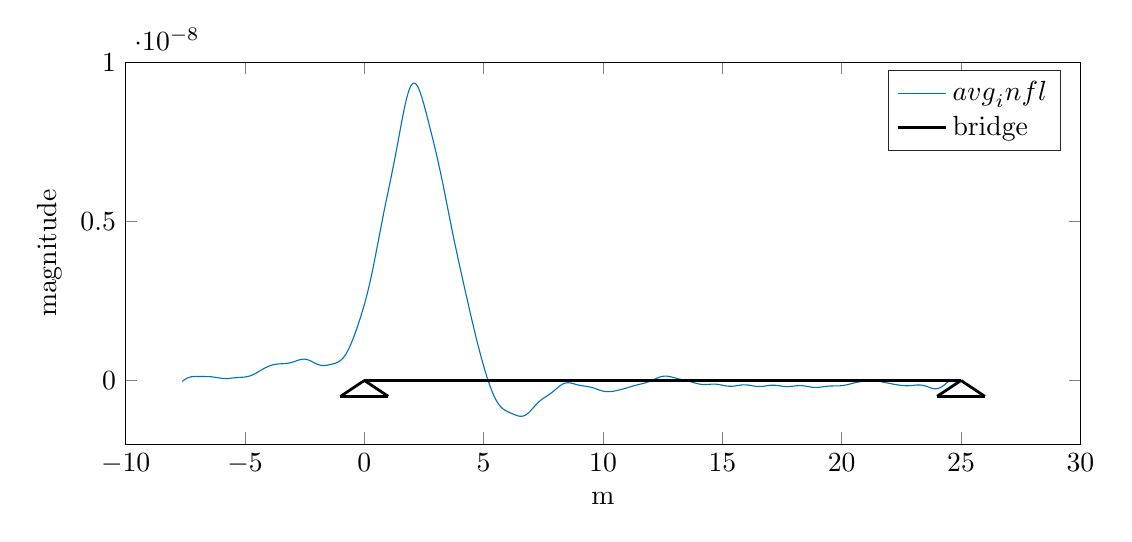
\begin{tikzpicture}

\begin{axis}[%
width=\textwidth,
height=0.4\textwidth,
at={(0\textwidth,0\textwidth)},
scale only axis,
xmin=-10,
xmax=30,
xlabel={m},
ymin=-2e-09,
ymax=1e-08,
ylabel={magnitude},
axis background/.style={fill=white},
title style={font=\bfseries},
title={},
legend style={legend cell align=left,align=left,draw=white!15!black}
]
\addplot [color=mycolor1,solid]
  table[row sep=crcr]{%
-7.62757577636719	-2.79121997927881e-11\\
-7.60746692382812	-1.62204102737836e-11\\
-7.58735807128906	-4.82853742552238e-12\\
-7.56724921875	6.2175604692499e-12\\
-7.54714036621094	1.6875941300512e-11\\
-7.52703151367187	2.71088835256999e-11\\
-7.50692266113281	3.68831406303935e-11\\
-7.48681380859375	4.61701432909534e-11\\
-7.46670495605469	5.49461475252258e-11\\
-7.44659610351562	6.31923277860747e-11\\
-7.42648725097656	7.08948146309099e-11\\
-7.4063783984375	7.80446772797448e-11\\
-7.38626954589844	8.46378520461286e-11\\
-7.36616069335937	9.06750182803034e-11\\
-7.34605184082031	9.61614240943953e-11\\
-7.32594298828125	1.011066647368e-10\\
-7.30583413574219	1.0552441703956e-10\\
-7.28572528320312	1.09432133871753e-10\\
-7.26561643066406	1.12850702986785e-10\\
-7.245507578125	1.15804075046708e-10\\
-7.22539872558594	1.18318865937226e-10\\
-7.20528987304687	1.20423938748983e-10\\
-7.18518102050781	1.22149970990877e-10\\
-7.16507216796875	1.2352901271758e-10\\
-7.14496331542969	1.24594041294948e-10\\
-7.12485446289062	1.25378518493554e-10\\
-7.10474561035156	1.25915955493018e-10\\
-7.0846367578125	1.26239491200123e-10\\
-7.06452790527344	1.2638148903478e-10\\
-7.04441905273437	1.26373157023373e-10\\
-7.02431020019531	1.26244195663798e-10\\
-7.00420134765625	1.26022477595751e-10\\
-6.98409249511719	1.2573376263001e-10\\
-6.96398364257812	1.25401451168175e-10\\
-6.94387479003906	1.2504637848696e-10\\
-6.9237659375	1.24686651776706e-10\\
-6.90365708496094	1.24337531219959e-10\\
-6.88354823242187	1.24011355781559e-10\\
-6.86343937988281	1.2371751376482e-10\\
-6.84333052734375	1.23462457577473e-10\\
-6.82322167480469	1.23249761554696e-10\\
-6.80311282226562	1.23080221112232e-10\\
-6.78300396972656	1.22951990958661e-10\\
-6.7628951171875	1.22860759588855e-10\\
-6.74278626464844	1.22799956817844e-10\\
-6.72267741210937	1.22760990701132e-10\\
-6.70256855957031	1.22733509829737e-10\\
-6.68245970703125	1.22705686690005e-10\\
-6.66235085449219	1.22664517543367e-10\\
-6.64224200195312	1.22596134112317e-10\\
-6.62213314941406	1.22486122257863e-10\\
-6.602024296875	1.22319842801213e-10\\
-6.58191544433594	1.22082749678528e-10\\
-6.56180659179687	1.21760700721017e-10\\
-6.54169773925781	1.21340256521521e-10\\
-6.52158888671875	1.20808963079903e-10\\
-6.50148003417969	1.20155614209626e-10\\
-6.48137118164062	1.19370490031815e-10\\
-6.46126232910156	1.18445568275878e-10\\
-6.4411534765625	1.17374705541453e-10\\
-6.42104462402344	1.16153786148112e-10\\
-6.40093577148437	1.14780836700633e-10\\
-6.38082691894531	1.13256105020503e-10\\
-6.36071806640625	1.11582102631921e-10\\
-6.34060921386719	1.0976361053433e-10\\
-6.32050036132812	1.07807648536335e-10\\
-6.30039150878906	1.05723408959518e-10\\
-6.28028265625	1.03522156037797e-10\\
-6.26017380371094	1.01217092831463e-10\\
-6.24006495117187	9.88231979375398e-11\\
-6.21995609863281	9.63570347040079e-11\\
-6.19984724609375	9.38365360379727e-11\\
-6.17973839355469	9.12807682327618e-11\\
-6.15962954101562	8.87096775211216e-11\\
-6.13952068847656	8.61438232879197e-11\\
-6.1194118359375	8.3604102042882e-11\\
-6.09930298339844	8.11114663602583e-11\\
-6.07919413085937	7.86866430365729e-11\\
-6.05908527832031	7.6349854699833e-11\\
-6.03897642578125	7.41205490242306e-11\\
-6.01886757324219	7.20171395652635e-11\\
-5.99875872070312	7.00567620337851e-11\\
-5.97864986816406	6.82550495766181e-11\\
-5.958541015625	6.66259303309167e-11\\
-5.93843216308594	6.51814501730048e-11\\
-5.91832331054687	6.39316231963458e-11\\
-5.89821445800781	6.28843120327713e-11\\
-5.87810560546875	6.20451396828597e-11\\
-5.85799675292969	6.141743405168e-11\\
-5.83788790039062	6.1002205902621e-11\\
-5.81777904785156	6.07981604508599e-11\\
-5.7976701953125	6.08017423273928e-11\\
-5.77756134277344	6.10072131606196e-11\\
-5.75745249023437	6.1406760552937e-11\\
-5.73734363769531	6.19906367807415e-11\\
-5.71723478515625	6.27473251246376e-11\\
-5.69712593261719	6.36637313476994e-11\\
-5.67701708007812	6.47253974893898e-11\\
-5.65690822753906	6.59167348355822e-11\\
-5.636799375	6.72212726652768e-11\\
-5.61669052246094	6.86219191655061e-11\\
-5.59658166992187	7.01012307502581e-11\\
-5.57647281738281	7.1641685918702e-11\\
-5.55636396484375	7.32259597437872e-11\\
-5.53625511230469	7.48371950944616e-11\\
-5.51614625976562	7.64592667628931e-11\\
-5.49603740722656	7.80770347903818e-11\\
-5.4759285546875	7.96765834603838e-11\\
-5.45581970214844	8.12454426508915e-11\\
-5.43571084960937	8.27727885078384e-11\\
-5.41560199707031	8.4249620711909e-11\\
-5.39549314453125	8.56689139583428e-11\\
-5.37538429199219	8.70257416474987e-11\\
-5.35527543945312	8.83173701875518e-11\\
-5.33516658691406	8.95433227335871e-11\\
-5.315057734375	9.07054116229798e-11\\
-5.29494888183594	9.18077392094783e-11\\
-5.27484002929687	9.28566672405541e-11\\
-5.25473117675781	9.38607553586551e-11\\
-5.23462232421875	9.48306697303016e-11\\
-5.21451347167969	9.57790632117058e-11\\
-5.19440461914062	9.67204288398719e-11\\
-5.17429576660156	9.76709287890201e-11\\
-5.1541869140625	9.864820124852e-11\\
-5.13407806152344	9.96711479563634e-11\\
-5.11396920898437	1.00759705357925e-10\\
-5.09386035644531	1.01934602550221e-10\\
-5.07375150390625	1.03217109315136e-10\\
-5.05364265136719	1.04628777639376e-10\\
-5.03353379882812	1.06191180163707e-10\\
-5.01342494628906	1.07925648999047e-10\\
-4.99331609375	1.09853018293294e-10\\
-4.97320724121094	1.1199337383148e-10\\
-4.95309838867187	1.14365812805407e-10\\
-4.93298953613281	1.16988216699921e-10\\
-4.91288068359375	1.19877040014977e-10\\
-4.89277183105469	1.23047117279553e-10\\
-4.87266297851562	1.26511490519689e-10\\
-4.85255412597656	1.30281259023481e-10\\
-4.8324452734375	1.3436545290558e-10\\
-4.81233642089844	1.3877093161858e-10\\
-4.79222756835937	1.43502308193745e-10\\
-4.77211871582031	1.48561899624701e-10\\
-4.75200986328125	1.53949703440752e-10\\
-4.73190101074219	1.59663400156635e-10\\
-4.71179215820312	1.65698380938461e-10\\
-4.69168330566406	1.72047799496158e-10\\
-4.671574453125	1.78702646905736e-10\\
-4.65146560058594	1.8565184778463e-10\\
-4.63135674804687	1.928823759936e-10\\
-4.61124789550781	2.00379387823096e-10\\
-4.59113904296875	2.08126370442817e-10\\
-4.57103019042969	2.16105303252661e-10\\
-4.55092133789062	2.24296829672965e-10\\
-4.53081248535156	2.32680436852331e-10\\
-4.5107036328125	2.41234640752734e-10\\
-4.49059478027344	2.49937174093373e-10\\
-4.47048592773437	2.58765174695549e-10\\
-4.45037707519531	2.67695371868991e-10\\
-4.43026822265625	2.76704268613e-10\\
-4.41015937011719	2.85768317570498e-10\\
-4.39005051757812	2.94864088866184e-10\\
-4.36994166503906	3.03968428177531e-10\\
-4.3498328125	3.13058603625055e-10\\
-4.32972395996094	3.22112440321559e-10\\
-4.30961510742187	3.31108441684287e-10\\
-4.28950625488281	3.40025896884068e-10\\
-4.26939740234375	3.48844974076635e-10\\
-4.24928854980469	3.57546799328802e-10\\
-4.22917969726562	3.6611352141093e-10\\
-4.20907084472656	3.74528362872689e-10\\
-4.1889619921875	3.82775658047504e-10\\
-4.16885313964844	3.90840878837845e-10\\
-4.14874428710937	3.98710649315784e-10\\
-4.12863543457031	4.06372750327297e-10\\
-4.10852658203125	4.13816115412947e-10\\
-4.08841772949219	4.21030819449057e-10\\
-4.06830887695312	4.28008061471742e-10\\
-4.04820002441406	4.34740143169858e-10\\
-4.028091171875	4.41220444522636e-10\\
-4.00798231933594	4.47443398013331e-10\\
-3.98787346679687	4.53404462773608e-10\\
-3.96776461425781	4.59100099905796e-10\\
-3.94765576171875	4.64527750094313e-10\\
-3.92754690917969	4.69685814456255e-10\\
-3.90743805664062	4.74573639397862e-10\\
-3.88732920410156	4.79191506041962e-10\\
-3.8672203515625	4.83540624576014e-10\\
-3.84711149902344	4.87623133645195e-10\\
-3.82700264648437	4.91442104684978e-10\\
-3.80689379394531	4.95001550857621e-10\\
-3.78678494140625	4.98306440031644e-10\\
-3.76667608886719	5.01362711027663e-10\\
-3.74656723632812	5.04177292152508e-10\\
-3.72645838378906	5.06758120860828e-10\\
-3.70634953125	5.09114163223464e-10\\
-3.68624067871094	5.1125543174884e-10\\
-3.66613182617187	5.13193000000412e-10\\
-3.64602297363281	5.14939012383065e-10\\
-3.62591412109375	5.16506687436358e-10\\
-3.60580526855469	5.17910312974307e-10\\
-3.58569641601562	5.19165231451234e-10\\
-3.56558756347656	5.2028781401113e-10\\
-3.5454787109375	5.21295421793962e-10\\
-3.52536985839844	5.22206353225062e-10\\
-3.50526100585937	5.23039776201723e-10\\
-3.48515215332031	5.23815644311717e-10\\
-3.46504330078125	5.24554596468821e-10\\
-3.44493444824219	5.25277839626832e-10\\
-3.42482559570312	5.2600701453175e-10\\
-3.40471674316406	5.26764044787184e-10\\
-3.384607890625	5.27570969835495e-10\\
-3.36449903808594	5.28449762791125e-10\\
-3.34439018554687	5.29422134397514e-10\\
-3.32428133300781	5.30509324708917e-10\\
-3.30417248046875	5.31731884417313e-10\\
-3.28406362792969	5.33109448046837e-10\\
-3.26395477539062	5.34660501517531e-10\\
-3.24384592285156	5.36402146831614e-10\\
-3.2237370703125	5.38349866853032e-10\\
-3.20362821777344	5.4051729333083e-10\\
-3.18351936523437	5.42915981453523e-10\\
-3.16341051269531	5.4555519431216e-10\\
-3.14330166015625	5.48441700690745e-10\\
-3.12319280761719	5.51579589591676e-10\\
-3.10308395507812	5.54970104839412e-10\\
-3.08297510253906	5.58611502986757e-10\\
-3.06286625	5.62498937575161e-10\\
-3.04275739746094	5.66624372573892e-10\\
-3.02264854492187	5.70976527544958e-10\\
-3.00253969238281	5.75540856753589e-10\\
-2.98243083984375	5.80299564071552e-10\\
-2.96232198730469	5.85231655106716e-10\\
-2.94221313476562	5.90313027542226e-10\\
-2.92210428222656	5.95516600187906e-10\\
-2.9019954296875	6.00812480741688e-10\\
-2.88188657714844	6.061681717363e-10\\
-2.86177772460937	6.11548813614113e-10\\
-2.84166887207031	6.16917463337742e-10\\
-2.82156001953125	6.22235406414173e-10\\
-2.80145116699219	6.27462499693665e-10\\
-2.78134231445312	6.32557541808846e-10\\
-2.76123346191406	6.37478667653042e-10\\
-2.741124609375	6.42183762866564e-10\\
-2.72101575683594	6.46630893913208e-10\\
-2.70090690429687	6.50778748993041e-10\\
-2.68079805175781	6.54587084757906e-10\\
-2.66068919921875	6.58017173578161e-10\\
-2.64058034667969	6.61032245957947e-10\\
-2.62047149414062	6.63597922615231e-10\\
-2.60036264160156	6.6568263073482e-10\\
-2.5802537890625	6.6725799896964e-10\\
-2.56014493652344	6.68299225907921e-10\\
-2.54003608398437	6.68785416942105e-10\\
-2.51992723144531	6.68699884766844e-10\\
-2.49981837890625	6.68030409096934e-10\\
-2.47970952636719	6.66769451626924e-10\\
-2.45960067382812	6.64914322748518e-10\\
-2.43949182128906	6.62467297093694e-10\\
-2.41938296875	6.59435675574385e-10\\
-2.39927411621094	6.55831792236048e-10\\
-2.37916526367187	6.51672964924499e-10\\
-2.35905641113281	6.46981389474069e-10\\
-2.33894755859375	6.4178397785103e-10\\
-2.31883870605469	6.3611214141993e-10\\
-2.29872985351562	6.30001521231407e-10\\
-2.27862100097656	6.23491667948595e-10\\
-2.2585121484375	6.16625674724776e-10\\
-2.23840329589844	6.09449767007789e-10\\
-2.21829444335937	6.0201285386691e-10\\
-2.19818559082031	5.9436604600648e-10\\
-2.17807673828125	5.8656214613841e-10\\
-2.15796788574219	5.78655117825322e-10\\
-2.13785903320312	5.70699539269896e-10\\
-2.11775018066406	5.62750048808219e-10\\
-2.097641328125	5.54860789060021e-10\\
-2.07753247558594	5.47084856793164e-10\\
-2.05742362304687	5.39473765570233e-10\\
-2.03731477050781	5.32076928160719e-10\\
-2.01720591796875	5.24941165522275e-10\\
-1.99709706542969	5.18110248880603e-10\\
-1.97698821289062	5.11624481071544e-10\\
-1.95687936035156	5.05520322855408e-10\\
-1.9367705078125	4.9983006937676e-10\\
-1.91666165527344	4.94581581329858e-10\\
-1.89655280273437	4.89798074707583e-10\\
-1.87644395019531	4.8549797226881e-10\\
-1.85633509765625	4.81694819065162e-10\\
-1.83622624511719	4.78397263533233e-10\\
-1.81611739257812	4.75609104793624e-10\\
-1.79600854003906	4.73329405915238e-10\\
-1.7758996875	4.71552672013937e-10\\
-1.75579083496094	4.70269091171179e-10\\
-1.73568198242187	4.69464835292915e-10\\
-1.71557312988281	4.69122417193951e-10\\
-1.69546427734375	4.69221099399791e-10\\
-1.67535542480469	4.69737349418563e-10\\
-1.65524657226562	4.70645335560307e-10\\
-1.63513771972656	4.71917456779928e-10\\
-1.6150288671875	4.7352489950264e-10\\
-1.59492001464844	4.75438213964511e-10\\
-1.57481116210937	4.7762790227293e-10\\
-1.55470230957031	4.80065010167885e-10\\
-1.53459345703125	4.8272171434876e-10\\
-1.51448460449219	4.85571897226234e-10\\
-1.49437575195312	4.88591701065305e-10\\
-1.47426689941406	4.91760053703697e-10\\
-1.454158046875	4.95059158357478e-10\\
-1.43404919433594	4.98474940459721e-10\\
-1.41394034179687	5.01997445012928e-10\\
-1.39383148925781	5.05621178565778e-10\\
-1.37372263671875	5.09345390641307e-10\\
-1.35361378417969	5.13174290238049e-10\\
-1.33350493164062	5.17117193887517e-10\\
-1.31339607910156	5.21188602669382e-10\\
-1.2932872265625	5.25408206547657e-10\\
-1.27317837402344	5.29800815383928e-10\\
-1.25306952148437	5.34396216994018e-10\\
-1.23296066894531	5.3922896362822e-10\\
-1.21285181640625	5.44338089258397e-10\\
-1.19274296386719	5.49766761033984e-10\\
-1.17263411132812	5.55561869208968e-10\\
-1.15252525878906	5.61773560730201e-10\\
-1.13241640625	5.68454722500989e-10\\
-1.11230755371094	5.75660421080449e-10\\
-1.09219870117187	5.8344730623805e-10\\
-1.07208984863281	5.91872986343586e-10\\
-1.05198099609375	6.00995384027285e-10\\
-1.03187214355469	6.10872080885118e-10\\
-1.01176329101562	6.21559660225436e-10\\
-0.991654438476562	6.33113056950032e-10\\
-0.971545585937499	6.45584923633808e-10\\
-0.951436733398437	6.59025021711182e-10\\
-0.931327880859374	6.73479646395611e-10\\
-0.911219028320312	6.88991093553777e-10\\
-0.891110175781249	7.05597176232799e-10\\
-0.871001323242187	7.23330797903397e-10\\
-0.850892470703124	7.42219588742364e-10\\
-0.830783618164062	7.6228561044323e-10\\
-0.810674765625	7.83545134125644e-10\\
-0.790565913085937	8.06008494923661e-10\\
-0.770457060546875	8.29680025784293e-10\\
-0.750348208007812	8.54558071914347e-10\\
-0.73023935546875	8.80635086190566e-10\\
-0.710130502929687	9.07897804711253e-10\\
-0.690021650390625	9.36327500532234e-10\\
-0.669912797851562	9.65900312512361e-10\\
-0.6498039453125	9.96587645109644e-10\\
-0.629695092773437	1.02835663393388e-09\\
-0.609586240234375	1.06117067089018e-09\\
-0.589477387695312	1.09498998185469e-09\\
-0.56936853515625	1.12977224902155e-09\\
-0.549259682617187	1.16547326936181e-09\\
-0.529150830078124	1.20204764005006e-09\\
-0.509041977539062	1.2394494612537e-09\\
-0.488933124999999	1.27763304634899e-09\\
-0.468824272460937	1.3165536294348e-09\\
-0.448715419921874	1.3561680599618e-09\\
-0.428606567382812	1.39643547438496e-09\\
-0.408497714843749	1.43731793497971e-09\\
-0.388388862304687	1.47878102633607e-09\\
-0.368280009765624	1.52079440055547e-09\\
-0.348171157226562	1.56333226281715e-09\\
-0.328062304687499	1.60637378974614e-09\\
-0.307953452148437	1.64990347389434e-09\\
-0.287844599609374	1.69391138862817e-09\\
-0.267735747070312	1.73839336878824e-09\\
-0.247626894531249	1.78335110363468e-09\\
-0.227518041992187	1.82879213980019e-09\\
-0.207409189453124	1.87472979322603e-09\\
-0.187300336914062	1.92118297033618e-09\\
-0.167191484375	1.9681758999953e-09\\
-0.147082631835937	2.01573777907756e-09\\
-0.126973779296875	2.06390233572936e-09\\
-0.106864926757812	2.11270731562099e-09\\
-0.0867560742187496	2.16219389763271e-09\\
-0.0666472216796867	2.21240604649398e-09\\
-0.0465383691406247	2.26338981087379e-09\\
-0.0264295166015618	2.31519257629176e-09\\
-0.00632066406249976	2.36786228296937e-09\\
0.0137881884765632	2.42144661935836e-09\\
0.0338970410156252	2.47599220255722e-09\\
0.0540058935546881	2.53154375715044e-09\\
0.0741147460937501	2.58814330417113e-09\\
0.094223598632813	2.64582937189357e-09\\
0.114332451171876	2.70463624000421e-09\\
0.134441303710938	2.76459322838068e-09\\
0.154550156250001	2.82572404122845e-09\\
0.174659008789063	2.88804617669108e-09\\
0.194767861328126	2.95157041126817e-09\\
0.214876713867188	3.01630036745458e-09\\
0.234985566406251	3.08223217196707e-09\\
0.255094418945313	3.14935421076216e-09\\
0.275203271484376	3.217646985787e-09\\
0.295312124023438	3.28708307705976e-09\\
0.315420976562501	3.35762721226423e-09\\
0.335529829101563	3.42923644458421e-09\\
0.355638681640626	3.50186043801581e-09\\
0.375747534179689	3.57544185790023e-09\\
0.395856386718751	3.64991686293581e-09\\
0.415965239257813	3.72521569347671e-09\\
0.436074091796876	3.80126334952666e-09\\
0.456182944335938	3.87798035050848e-09\\
0.476291796875	3.95528356765375e-09\\
0.496400649414062	4.03308711872821e-09\\
0.516509501953126	4.11130331380451e-09\\
0.536618354492188	4.1898436399297e-09\\
0.55672720703125	4.26861977182314e-09\\
0.576836059570312	4.34754459519228e-09\\
0.596944912109376	4.42653322887944e-09\\
0.617053764648438	4.50550403185735e-09\\
0.6371626171875	4.58437958108072e-09\\
0.657271469726562	4.66308760637747e-09\\
0.677380322265626	4.7415618689251e-09\\
0.697489174804688	4.81974297040372e-09\\
0.71759802734375	4.89757908064093e-09\\
0.737706879882812	4.97502657245811e-09\\
0.757815732421876	5.05205055348212e-09\\
0.777924584960938	5.12862528588967e-09\\
0.7980334375	5.20473448638783e-09\\
0.818142290039064	5.28037150018882e-09\\
0.838251142578126	5.35553934429134e-09\\
0.858359995117188	5.43025061701513e-09\\
0.87846884765625	5.50452727243011e-09\\
0.898577700195314	5.57840026005408e-09\\
0.918686552734376	5.65190903194199e-09\\
0.938795405273438	5.72510092103246e-09\\
0.9589042578125	5.79803039633039e-09\\
0.979013110351564	5.87075820216663e-09\\
0.999121962890626	5.94335039036395e-09\\
1.01923081542969	6.015877255632e-09\\
1.03933966796875	6.08841218589302e-09\\
1.05944852050781	6.16103044048513e-09\\
1.07955737304688	6.23380787028465e-09\\
1.09966622558594	6.30681959471745e-09\\
1.119775078125	6.38013865137856e-09\\
1.13988393066406	6.45383463453809e-09\\
1.15999278320313	6.52797233917174e-09\\
1.18010163574219	6.60261042730858e-09\\
1.20021048828125	6.67780013343536e-09\\
1.22031934082031	6.7535840254328e-09\\
1.24042819335938	6.8299948370486e-09\\
1.26053704589844	6.9070543872371e-09\\
1.2806458984375	6.98477260082535e-09\\
1.30075475097656	7.06314664390801e-09\\
1.32086360351563	7.14216018614238e-09\\
1.34097245605469	7.22178280072308e-09\\
1.36108130859375	7.30196951128117e-09\\
1.38119016113281	7.38266049329227e-09\\
1.40129901367188	7.46378093581281e-09\\
1.42140786621094	7.54524106751517e-09\\
1.44151671875	7.62693634908196e-09\\
1.46162557128906	7.70874783207292e-09\\
1.48173442382812	7.7905426824168e-09\\
1.50184327636719	7.87217486473064e-09\\
1.52195212890625	7.95348598175391e-09\\
1.54206098144531	8.03430626132903e-09\\
1.56216983398437	8.11445568158574e-09\\
1.58227868652344	8.19374522331715e-09\\
1.6023875390625	8.27197823699083e-09\\
1.62249639160156	8.34895191043849e-09\\
1.64260524414062	8.42445882203006e-09\\
1.66271409667969	8.49828856307818e-09\\
1.68282294921875	8.57022941235046e-09\\
1.70293180175781	8.64007004490015e-09\\
1.72304065429688	8.70760125697022e-09\\
1.74314950683594	8.77261768848611e-09\\
1.763258359375	8.83491952463255e-09\\
1.78336721191406	8.89431415820967e-09\\
1.80347606445313	8.95061779488104e-09\\
1.82358491699219	9.0036569840558e-09\\
1.84369376953125	9.05327005898122e-09\\
1.86380262207031	9.09930847065035e-09\\
1.88391147460938	9.14163800133911e-09\\
1.90402032714844	9.18013984496299e-09\\
1.9241291796875	9.21471154296883e-09\\
1.94423803222656	9.24526776613292e-09\\
1.96434688476563	9.27174093440134e-09\\
1.98445573730469	9.29408166876243e-09\\
2.00456458984375	9.31225907105886e-09\\
2.02467344238281	9.32626082960674e-09\\
2.04478229492188	9.33609315046586e-09\\
2.06489114746094	9.34178051617531e-09\\
2.085	9.3433652757071e-09\\
2.10510885253906	9.34090707127535e-09\\
2.12521770507813	9.33448210944482e-09\\
2.14532655761719	9.32418228569075e-09\\
2.16543541015625	9.31011417314994e-09\\
2.18554426269531	9.2923978877532e-09\\
2.20565311523438	9.27116584322358e-09\\
2.22576196777344	9.2465614105498e-09\\
2.2458708203125	9.21873749748575e-09\\
2.26597967285156	9.1878550643753e-09\\
2.28608852539063	9.15408159314988e-09\\
2.30619737792969	9.11758952668694e-09\\
2.32630623046875	9.07855469585062e-09\\
2.34641508300781	9.0371547514597e-09\\
2.36652393554688	8.99356761814566e-09\\
2.38663278808594	8.94796998658123e-09\\
2.406741640625	8.90053585988364e-09\\
2.42685049316406	8.85143516913854e-09\\
2.44695934570313	8.80083247196174e-09\\
2.46706819824219	8.74888574683081e-09\\
2.48717705078125	8.69574529459488e-09\\
2.50728590332031	8.64155275712462e-09\\
2.52739475585938	8.58644026151658e-09\\
2.54750360839844	8.53052969663654e-09\\
2.5676124609375	8.47393212709583e-09\\
2.58772131347656	8.41674734802677e-09\\
2.60783016601563	8.35906358227798e-09\\
2.62793901855469	8.30095731991174e-09\\
2.64804787109375	8.24249329817441e-09\\
2.66815672363281	8.18372461844907e-09\\
2.68826557617188	8.12469299510689e-09\\
2.70837442871094	8.06542912967043e-09\\
2.72848328125	8.00595320230509e-09\\
2.74859213378906	7.94627547138152e-09\\
2.76870098632812	7.88639697071591e-09\\
2.78880983886719	7.82631029310962e-09\\
2.80891869140625	7.76600044798538e-09\\
2.82902754394531	7.70544578026164e-09\\
2.84913639648437	7.64461893712696e-09\\
2.86924524902344	7.58348786907497e-09\\
2.8893541015625	7.522016851439e-09\\
2.90946295410156	7.46016751272369e-09\\
2.92957180664062	7.39789985626352e-09\\
2.94968065917969	7.33517326214117e-09\\
2.96978951171875	7.27194745686309e-09\\
2.98989836425781	7.20818343900568e-09\\
3.01000721679688	7.14384434990171e-09\\
3.03011606933594	7.07889627941879e-09\\
3.050224921875	7.01330899797567e-09\\
3.07033377441406	6.94705660713046e-09\\
3.09044262695313	6.88011810234122e-09\\
3.11055147949219	6.81247784282508e-09\\
3.13066033203125	6.74412592480808e-09\\
3.15076918457031	6.67505845584622e-09\\
3.17087803710938	6.60527772928883e-09\\
3.19098688964844	6.53479229932979e-09\\
3.2110957421875	6.46361695843266e-09\\
3.23120459472656	6.39177262020399e-09\\
3.25131344726563	6.31928611200866e-09\\
3.27142229980469	6.24618988275756e-09\\
3.29153115234375	6.17252163233512e-09\\
3.31164000488281	6.0983238700625e-09\\
3.33174885742188	6.0236434103981e-09\\
3.35185770996094	5.94853081475359e-09\\
3.3719665625	5.87303978884278e-09\\
3.39207541503906	5.79722654537766e-09\\
3.41218426757813	5.72114914217796e-09\\
3.43229312011719	5.64486680586671e-09\\
3.45240197265625	5.56843925128559e-09\\
3.47251082519531	5.49192600658344e-09\\
3.49261967773438	5.41538575361454e-09\\
3.51272853027344	5.3388756928372e-09\\
3.5328373828125	5.26245094133535e-09\\
3.55294623535156	5.18616397190858e-09\\
3.57305508789063	5.11006410039864e-09\\
3.59316394042969	5.03419702755764e-09\\
3.61327279296875	4.95860444082752e-09\\
3.63338164550781	4.88332368040776e-09\\
3.65349049804688	4.80838747295278e-09\\
3.67359935058594	4.73382373517878e-09\\
3.693708203125	4.65965544858731e-09\\
3.71381705566406	4.58590060544474e-09\\
3.73392590820313	4.51257222510992e-09\\
3.75403476074219	4.43967843878974e-09\\
3.77414361328125	4.36722263983974e-09\\
3.79425246582031	4.29520369582634e-09\\
3.81436131835938	4.22361621774197e-09\\
3.83447017089844	4.15245088102379e-09\\
3.8545790234375	4.08169479238168e-09\\
3.87468787597656	4.0113318958983e-09\\
3.89479672851563	3.9413434114307e-09\\
3.91490558105469	3.87170829802257e-09\\
3.93501443359375	3.80240373483279e-09\\
3.95512328613281	3.73340561199923e-09\\
3.97523213867188	3.66468902388726e-09\\
3.99534099121094	3.59622875731675e-09\\
4.01544984375	3.52799976761579e-09\\
4.03555869628906	3.45997763570845e-09\\
4.05566754882812	3.39213899989958e-09\\
4.07577640136719	3.32446195656462e-09\\
4.09588525390625	3.25692642457556e-09\\
4.11599410644531	3.18951446898579e-09\\
4.13610295898437	3.12221058024418e-09\\
4.15621181152344	3.05500190600019e-09\\
4.1763206640625	2.98787843338436e-09\\
4.19642951660156	2.92083312048851e-09\\
4.21653836914062	2.85386197661437e-09\\
4.23664722167969	2.78696409169474e-09\\
4.25675607421875	2.72014161610508e-09\\
4.27686492675781	2.65339969286233e-09\\
4.29697377929688	2.58674634494105e-09\\
4.31708263183594	2.52019232111296e-09\\
4.337191484375	2.45375090432475e-09\\
4.35730033691406	2.38743768716236e-09\\
4.37740918945313	2.32127031939973e-09\\
4.39751804199219	2.25526823299013e-09\\
4.41762689453125	2.18945235012455e-09\\
4.43773574707031	2.12384478015023e-09\\
4.45784459960938	2.05846851121219e-09\\
4.47795345214844	1.99334710245137e-09\\
4.4980623046875	1.92850438246604e-09\\
4.51817115722656	1.86396415952187e-09\\
4.53828000976563	1.79974994868456e-09\\
4.55838886230469	1.73588472065312e-09\\
4.57849771484375	1.67239067659962e-09\\
4.59860656738281	1.6092890527794e-09\\
4.61871541992188	1.54659995807541e-09\\
4.63882427246094	1.48434224699029e-09\\
4.658933125	1.42253342991198e-09\\
4.67904197753906	1.36118962176397e-09\\
4.69915083007813	1.30032552942232e-09\\
4.71925968261719	1.23995447754893e-09\\
4.73936853515625	1.18008847176891e-09\\
4.75947738769531	1.1207382974175e-09\\
4.77958624023438	1.06191365141429e-09\\
4.79969509277344	1.00362330419695e-09\\
4.8198039453125	9.45875288075912e-10\\
4.83991279785156	8.8867710786374e-10\\
4.86002165039063	8.3203596919646e-10\\
4.88013050292969	7.75959019606916e-10\\
4.90023935546875	7.20453597137305e-10\\
4.92034820800781	6.655274810946e-10\\
4.94045706054688	6.11189139461447e-10\\
4.96056591308594	5.5744796747821e-10\\
4.980674765625	5.04314512009194e-10\\
5.00078361816406	4.51800676496619e-10\\
5.02089247070313	3.99919901586716e-10\\
5.04100132324219	3.48687316879273e-10\\
5.06111017578125	2.98119859699586e-10\\
5.08121902832031	2.48236357313236e-10\\
5.10132788085938	1.99057569591215e-10\\
5.12143673339844	1.50606189777002e-10\\
5.1415455859375	1.0290680169789e-10\\
5.16165443847656	5.59857924895944e-11\\
5.18176329101563	9.87122065470039e-12\\
5.20187214355469	-3.54073599602061e-11\\
5.22198099609375	-7.98191189186944e-11\\
5.24208984863281	-1.23332208575914e-10\\
5.26219870117187	-1.65914061252654e-10\\
5.28230755371094	-2.0753172067165e-10\\
5.30241640625	-2.48152203476322e-10\\
5.32252525878906	-2.87742886059341e-10\\
5.34263411132812	-3.26271911402366e-10\\
5.36274296386719	-3.63708610177544e-10\\
5.38285181640625	-4.00023929993863e-10\\
5.40296066894531	-4.35190866393418e-10\\
5.42306952148437	-4.69184889019803e-10\\
5.44317837402344	-5.0198435629632e-10\\
5.4632872265625	-5.33570911968436e-10\\
5.48339607910156	-5.63929856983422e-10\\
5.50350493164062	-5.93050490399735e-10\\
5.52361378417969	-6.20926413337347e-10\\
5.54372263671875	-6.47555790394089e-10\\
5.56383148925781	-6.72941563456997e-10\\
5.58394034179688	-6.97091613425225e-10\\
5.60404919433594	-7.20018866024288e-10\\
5.624158046875	-7.41741338621505e-10\\
5.64426689941406	-7.6228212573911e-10\\
5.66437575195313	-7.81669321794125e-10\\
5.68448460449219	-7.9993588046039e-10\\
5.70459345703125	-8.17119410936502e-10\\
5.72470230957031	-8.33261912300581e-10\\
5.74481116210938	-8.48409448026069e-10\\
5.76492001464844	-8.62611763609174e-10\\
5.7850288671875	-8.75921851105244e-10\\
5.80513771972656	-8.88395465175799e-10\\
5.82524657226563	-9.00090595998112e-10\\
5.84535542480469	-9.1106690507404e-10\\
5.86546427734375	-9.21385130583634e-10\\
5.88557312988281	-9.3110646945249e-10\\
5.90568198242188	-9.40291943731839e-10\\
5.92579083496094	-9.49001759219697e-10\\
5.9458996875	-9.57294664474631e-10\\
5.96600854003906	-9.65227318486717e-10\\
5.98611739257813	-9.72853675270422e-10\\
6.00622624511719	-9.80224393530312e-10\\
6.02633509765625	-9.87386279323703e-10\\
6.04644395019531	-9.94381769306281e-10\\
6.06655280273438	-1.00124846170146e-09\\
6.08666165527344	-1.00801870158716e-09\\
6.1067705078125	-1.01471922645119e-09\\
6.12687936035156	-1.02137087723721e-09\\
6.14698821289063	-1.02798837929611e-09\\
6.16709706542969	-1.03458019678374e-09\\
6.18720591796875	-1.04114846311637e-09\\
6.20731477050781	-1.04768898912259e-09\\
6.22742362304688	-1.05419134952761e-09\\
6.24753247558594	-1.06063904738678e-09\\
6.267641328125	-1.06700975506287e-09\\
6.28775018066406	-1.07327562933121e-09\\
6.30785903320313	-1.07940369721088e-09\\
6.32796788574219	-1.08535630817282e-09\\
6.34807673828125	-1.09109164748084e-09\\
6.36818559082031	-1.09656430458964e-09\\
6.38829444335938	-1.10172588976883e-09\\
6.40840329589844	-1.10652569145249e-09\\
6.4285121484375	-1.11091136624061e-09\\
6.44862100097656	-1.1148296530092e-09\\
6.46872985351563	-1.11822710222729e-09\\
6.48883870605469	-1.12105081133674e-09\\
6.50894755859375	-1.1232491569277e-09\\
6.52905641113281	-1.1247725144422e-09\\
6.54916526367187	-1.12557395625974e-09\\
6.56927411621094	-1.12560991926168e-09\\
6.58938296875	-1.12484083333226e-09\\
6.60949182128906	-1.123231702729e-09\\
6.62960067382812	-1.12075263283819e-09\\
6.64970952636719	-1.11737929551375e-09\\
6.66981837890625	-1.11309332697256e-09\\
6.68992723144531	-1.10788265307467e-09\\
6.71003608398437	-1.10174173774263e-09\\
6.73014493652344	-1.09467175125715e-09\\
6.7502537890625	-1.08668065619498e-09\\
6.77036264160156	-1.07778320983328e-09\\
6.79047149414062	-1.06800088292148e-09\\
6.81058034667969	-1.05736169580013e-09\\
6.83068919921875	-1.04589997391331e-09\\
6.85079805175781	-1.03365602580238e-09\\
6.87090690429688	-1.02067574767015e-09\\
6.89101575683594	-1.00701015955266e-09\\
6.911124609375	-9.9271487901803e-10\\
6.93123346191406	-9.7784953911691e-10\\
6.95134231445313	-9.62477158024977e-10\\
6.97145116699219	-9.4666346843727e-10\\
6.99156001953125	-9.30476215286389e-10\\
7.01166887207031	-9.13984430756798e-10\\
7.03177772460938	-8.97257695849218e-10\\
7.05188657714844	-8.8036539790957e-10\\
7.0719954296875	-8.63375993573264e-10\\
7.09210428222656	-8.46356286488347e-10\\
7.11221313476563	-8.29370728970698e-10\\
7.13232198730469	-8.12480756414428e-10\\
7.15243083984375	-7.95744162835514e-10\\
7.17253969238281	-7.7921452537218e-10\\
7.19264854492188	-7.6294068490974e-10\\
7.21275739746094	-7.46966289248941e-10\\
7.23286625	-7.31329404405637e-10\\
7.25297510253906	-7.16062198727314e-10\\
7.27308395507813	-7.01190703550125e-10\\
7.29319280761719	-6.86734653112363e-10\\
7.31330166015625	-6.72707405399488e-10\\
7.33341051269531	-6.59115944536383e-10\\
7.35351936523438	-6.45960964278208e-10\\
7.37362821777344	-6.33237031096376e-10\\
7.3937370703125	-6.20932824324777e-10\\
7.41384592285156	-6.09031449836858e-10\\
7.43395477539063	-5.9751082277995e-10\\
7.45406362792969	-5.8634411401126e-10\\
7.47417248046875	-5.75500254072131e-10\\
7.49428133300781	-5.64944487813662e-10\\
7.51439018554688	-5.54638972156953e-10\\
7.53449903808594	-5.44543408943249e-10\\
7.554607890625	-5.34615704409343e-10\\
7.57471674316406	-5.24812646517376e-10\\
7.59482559570313	-5.1509059117866e-10\\
7.61493444824219	-5.05406148340943e-10\\
7.63504330078125	-4.95716858957386e-10\\
7.65515215332031	-4.85981854022949e-10\\
7.67526100585938	-4.76162487146258e-10\\
7.69536985839844	-4.66222932518917e-10\\
7.7154787109375	-4.56130740642988e-10\\
7.73558756347656	-4.45857344774603e-10\\
7.75569641601563	-4.35378511728193e-10\\
7.77580526855469	-4.2467473145264e-10\\
7.79591412109375	-4.13731540626809e-10\\
7.81602297363281	-4.02539776415691e-10\\
7.83613182617187	-3.91095757468342e-10\\
7.85624067871094	-3.79401390210948e-10\\
7.87634953125	-3.67464199480851e-10\\
7.89645838378906	-3.55297283545836e-10\\
7.91656723632812	-3.42919194544751e-10\\
7.93667608886719	-3.30353746357072e-10\\
7.95678494140625	-3.17629752847748e-10\\
7.97689379394531	-3.04780700327056e-10\\
7.99700264648437	-2.91844358901907e-10\\
8.01711149902344	-2.78862338164089e-10\\
8.0372203515625	-2.65879593352616e-10\\
8.05732920410156	-2.52943888732942e-10\\
8.07743805664062	-2.40105225448041e-10\\
8.09754690917969	-2.27415241508625e-10\\
8.11765576171875	-2.14926591897797e-10\\
8.13776461425781	-2.02692316965664e-10\\
8.15787346679688	-1.90765207379852e-10\\
8.17798231933594	-1.79197173878434e-10\\
8.198091171875	-1.68038629943322e-10\\
8.21820002441406	-1.57337895277461e-10\\
8.23830887695313	-1.47140627632002e-10\\
8.25841772949219	-1.37489290095551e-10\\
8.27852658203125	-1.28422660433079e-10\\
8.29863543457031	-1.1997538845479e-10\\
8.31874428710938	-1.12177606714312e-10\\
8.33885313964844	-1.05054599090481e-10\\
8.3589619921875	-9.8626531008199e-11\\
8.37907084472656	-9.29082442129367e-11\\
8.39917969726562	-8.79091181414918e-11\\
8.41928854980469	-8.36329990410809e-11\\
8.43939740234375	-8.00781970913959e-11\\
8.45950625488281	-7.72375508924391e-11\\
8.47961510742187	-7.50985578061506e-11\\
8.49972395996094	-7.36435677941617e-11\\
8.5198328125	-7.28500375879946e-11\\
8.53994166503906	-7.26908412726007e-11\\
8.56005051757812	-7.31346326684815e-11\\
8.58015937011719	-7.4146254270864e-11\\
8.60026822265625	-7.56871869539609e-11\\
8.62037707519531	-7.77160341810037e-11\\
8.64048592773437	-8.01890340819256e-11\\
8.66059478027344	-8.30605924742135e-11\\
8.6807036328125	-8.6283829711779e-11\\
8.70081248535156	-8.98111341528644e-11\\
8.72092133789062	-9.35947150415292e-11\\
8.74103019042969	-9.75871476967195e-11\\
8.76113904296875	-1.01741904096216e-10\\
8.78124789550781	-1.06013862225783e-10\\
8.80135674804687	-1.10359787932279e-10\\
8.82146560058594	-1.14738783466751e-10\\
8.841574453125	-1.19112697423198e-10\\
8.86168330566406	-1.23446491362499e-10\\
8.88179215820313	-1.27708559050278e-10\\
8.90190101074219	-1.31870994923264e-10\\
8.92200986328125	-1.35909809120476e-10\\
8.94211871582031	-1.39805087163698e-10\\
8.96222756835937	-1.43541093135312e-10\\
8.98233642089844	-1.4710631597018e-10\\
9.0024452734375	-1.50493459241387e-10\\
9.02255412597656	-1.5369937556693e-10\\
9.04266297851563	-1.56724947485827e-10\\
9.06277183105469	-1.59574917338279e-10\\
9.08288068359375	-1.62257669326321e-10\\
9.10298953613281	-1.64784967520844e-10\\
9.12309838867187	-1.67171654110564e-10\\
9.14320724121094	-1.69435312651953e-10\\
9.16331609375	-1.71595901470963e-10\\
9.18342494628906	-1.73675362683175e-10\\
9.20353379882813	-1.75697212535526e-10\\
9.22364265136719	-1.7768611892788e-10\\
9.24375150390625	-1.79667472045446e-10\\
9.26386035644531	-1.81666954023598e-10\\
9.28396920898437	-1.83710113476438e-10\\
9.30407806152344	-1.85821950551697e-10\\
9.3241869140625	-1.88026517931087e-10\\
9.34429576660156	-1.90346542881192e-10\\
9.36440461914063	-1.92803075081162e-10\\
9.38451347167969	-1.95415164515749e-10\\
9.40462232421875	-1.98199573232954e-10\\
9.42473117675781	-2.01170524232069e-10\\
9.44484002929687	-2.04339490178512e-10\\
9.46494888183594	-2.07715024044975e-10\\
9.485057734375	-2.11302633162942e-10\\
9.50516658691406	-2.15104697543293e-10\\
9.52527543945313	-2.1912043269877e-10\\
9.54538429199219	-2.23345896582908e-10\\
9.56549314453125	-2.27774039658637e-10\\
9.58560199707031	-2.32394796533041e-10\\
9.60571084960937	-2.37195217050509e-10\\
9.62581970214844	-2.42159634232104e-10\\
9.6459285546875	-2.47269865990475e-10\\
9.66603740722656	-2.52505447143248e-10\\
9.68614625976562	-2.57843887898037e-10\\
9.70625511230469	-2.63260954693333e-10\\
9.72636396484375	-2.68730969054413e-10\\
9.74647281738281	-2.74227119964376e-10\\
9.76658166992187	-2.79721785158372e-10\\
9.78669052246094	-2.85186856724437e-10\\
9.806799375	-2.90594066436007e-10\\
9.82690822753906	-2.95915306347571e-10\\
9.84701708007812	-3.01122940353322e-10\\
9.86712593261719	-3.06190102635351e-10\\
9.88723478515625	-3.11090979208915e-10\\
9.90734363769531	-3.15801069102154e-10\\
9.92745249023437	-3.20297422080972e-10\\
9.94756134277344	-3.24558850240106e-10\\
9.9676701953125	-3.28566111222302e-10\\
9.98777904785156	-3.32302061291634e-10\\
10.0078879003906	-3.35751776967448e-10\\
10.0279967529297	-3.38902644414428e-10\\
10.0481056054687	-3.41744416274753e-10\\
10.0682144580078	-3.44269236112886e-10\\
10.0883233105469	-3.46471631114899e-10\\
10.1084321630859	-3.48348474135903e-10\\
10.128541015625	-3.4989891661451e-10\\
10.1486498681641	-3.51124294266488e-10\\
10.1687587207031	-3.52028007825473e-10\\
10.1888675732422	-3.52615381412249e-10\\
10.2089764257812	-3.52893501381504e-10\\
10.2290852783203	-3.52871038713028e-10\\
10.2491941308594	-3.52558058180581e-10\\
10.2693029833984	-3.51965817644509e-10\\
10.2894118359375	-3.51106560872811e-10\\
10.3095206884766	-3.499933072999e-10\\
10.3296295410156	-3.4863964208345e-10\\
10.3497383935547	-3.47059509719553e-10\\
10.3698472460937	-3.45267014326823e-10\\
10.3899560986328	-3.43276229514714e-10\\
10.4100649511719	-3.41101020513798e-10\\
10.4301738037109	-3.38754880970459e-10\\
10.45028265625	-3.36250786500421e-10\\
10.4703915087891	-3.3360106676015e-10\\
10.4905003613281	-3.30817297438122e-10\\
10.5106092138672	-3.27910213195194e-10\\
10.5307180664062	-3.24889642201222e-10\\
10.5508269189453	-3.21764462529603e-10\\
10.5709357714844	-3.18542580288977e-10\\
10.5910446240234	-3.15230928997959e-10\\
10.6111534765625	-3.11835489350294e-10\\
10.6312623291016	-3.08361328179897e-10\\
10.6513711816406	-3.04812655123024e-10\\
10.6714800341797	-3.01192895192919e-10\\
10.6915888867187	-2.97504775235255e-10\\
10.7116977392578	-2.93750422023529e-10\\
10.7318065917969	-2.89931469586063e-10\\
10.7519154443359	-2.86049173231839e-10\\
10.772024296875	-2.82104527663347e-10\\
10.7921331494141	-2.78098386531352e-10\\
10.8122420019531	-2.7403158079929e-10\\
10.8323508544922	-2.69905033343258e-10\\
10.8524597070313	-2.65719867315874e-10\\
10.8725685595703	-2.61477505946652e-10\\
10.8926774121094	-2.57179761635304e-10\\
10.9127862646484	-2.5282891241423e-10\\
10.9328951171875	-2.48427764108505e-10\\
10.9530039697266	-2.43979696801705e-10\\
10.9731128222656	-2.39488694518961e-10\\
10.9932216748047	-2.34959357359852e-10\\
11.0133305273438	-2.30396895647553e-10\\
11.0334393798828	-2.258071060016e-10\\
11.0535482324219	-2.21196329584082e-10\\
11.0736570849609	-2.16571393107352e-10\\
11.0937659375	-2.11939533519952e-10\\
11.1138747900391	-2.07308307600857e-10\\
11.1339836425781	-2.02685487985439e-10\\
11.1540924951172	-1.98078947414673e-10\\
11.1742013476563	-1.93496533237961e-10\\
11.1943102001953	-1.88945934405134e-10\\
11.2144190527344	-1.84434543351973e-10\\
11.2345279052734	-1.79969315312465e-10\\
11.2546367578125	-1.75556627678251e-10\\
11.2747456103516	-1.71202142069613e-10\\
11.2948544628906	-1.66910671782077e-10\\
11.3149633154297	-1.62686057227992e-10\\
11.3350721679688	-1.58531051904061e-10\\
11.3551810205078	-1.54447221284714e-10\\
11.3752898730469	-1.50434856869333e-10\\
11.3953987255859	-1.46492907401405e-10\\
11.415507578125	-1.42618929032513e-10\\
11.4356164306641	-1.3880905592742e-10\\
11.4557252832031	-1.35057992502679e-10\\
11.4758341357422	-1.31359028164573e-10\\
11.4959429882813	-1.27704075067778e-10\\
11.5160518408203	-1.24083729059203e-10\\
11.5361606933594	-1.20487353607555e-10\\
11.5562695458984	-1.16903186153372e-10\\
11.5763783984375	-1.13318465953092e-10\\
11.5964872509766	-1.0971958213855e-10\\
11.6165961035156	-1.06092240376756e-10\\
11.6367049560547	-1.02421646198214e-10\\
11.6568138085938	-9.86927027707814e-11\\
11.6769226611328	-9.4890220634845e-11\\
11.6970315136719	-9.09991366879726e-11\\
11.7171403662109	-8.70047395176736e-11\\
11.73724921875	-8.28928980317685e-11\\
11.7573580712891	-7.86502902303887e-11\\
11.7774669238281	-7.42646289030259e-11\\
11.7975757763672	-6.97248810201404e-11\\
11.8176846289063	-6.50214776217586e-11\\
11.8377934814453	-6.0146511085363e-11\\
11.8579023339844	-5.50939167811983e-11\\
11.8780111865234	-4.98596362935691e-11\\
11.8981200390625	-4.44417595994367e-11\\
11.9182288916016	-3.88406438480537e-11\\
11.9383377441406	-3.3059006673953e-11\\
11.9584465966797	-2.71019922965442e-11\\
11.9785554492187	-2.09772090085243e-11\\
11.9986643017578	-1.46947370271987e-11\\
12.0187731542969	-8.26710607290919e-12\\
12.0388820068359	-1.70924244123638e-12\\
12.058990859375	4.96161425492015e-12\\
12.0790997119141	1.17260240867345e-11\\
12.0992085644531	1.85624885616087e-11\\
12.1193174169922	2.54476197379942e-11\\
12.1394262695312	3.23563349350278e-11\\
12.1595351220703	3.92620749110679e-11\\
12.1796439746094	4.61370430534958e-11\\
12.1997528271484	5.29524628216953e-11\\
12.2198616796875	5.96788504203889e-11\\
12.2399705322266	6.62862994549668e-11\\
12.2600793847656	7.27447741379191e-11\\
12.2801882373047	7.90244074780581e-11\\
12.3002970898437	8.50958007945854e-11\\
12.3204059423828	9.09303208570138e-11\\
12.3405147949219	9.65003909608886e-11\\
12.3606236474609	1.01779772307477e-10\\
12.3807325	1.06743832163156e-10\\
12.4008413525391	1.11369795429292e-10\\
12.4209502050781	1.15636976454142e-10\\
12.4410590576172	1.19526988162247e-10\\
12.4611679101562	1.23023925860304e-10\\
12.4812767626953	1.26114523398226e-10\\
12.5013856152344	1.28788279715525e-10\\
12.5214944677734	1.3103755418145e-10\\
12.5416033203125	1.32857629537649e-10\\
12.5617121728516	1.342467416689e-10\\
12.5818210253906	1.35206075855046e-10\\
12.6019298779297	1.35739729589894e-10\\
12.6220387304687	1.35854642484758e-10\\
12.6421475830078	1.35560494199517e-10\\
12.6622564355469	1.34869571756792e-10\\
12.6823652880859	1.33796607989753e-10\\
12.702474140625	1.3235859324543e-10\\
12.7225829931641	1.30574562808635e-10\\
12.7426918457031	1.28465362821703e-10\\
12.7628006982422	1.26053397748294e-10\\
12.7829095507812	1.23362362661821e-10\\
12.8030184033203	1.20416963827247e-10\\
12.8231272558594	1.17242631187159e-10\\
12.8432361083984	1.13865226456536e-10\\
12.8633449609375	1.10310750574983e-10\\
12.8834538134766	1.06605054259439e-10\\
12.9035626660156	1.02773555344728e-10\\
12.9236715185547	9.88409664948137e-11\\
12.9437803710937	9.48310367154217e-11\\
12.9638892236328	9.07663099012409e-11\\
12.9839980761719	8.66679034107801e-11\\
13.0041069287109	8.25553093824621e-11\\
13.02421578125	7.84462211905759e-11\\
13.0443246337891	7.43563870936872e-11\\
13.0644334863281	7.02994927554123e-11\\
13.0845423388672	6.62870739237033e-11\\
13.1046511914062	6.23284601447076e-11\\
13.1247600439453	5.84307499670299e-11\\
13.1448688964844	5.45988176669115e-11\\
13.1649777490234	5.08353511007612e-11\\
13.1850866015625	4.71409198738054e-11\\
13.2051954541016	4.35140726084274e-11\\
13.2253043066406	3.99514617080472e-11\\
13.2454131591797	3.64479936476696e-11\\
13.2655220117187	3.29970024850959e-11\\
13.2856308642578	2.95904439818066e-11\\
13.3057397167969	2.62191074537416e-11\\
13.3258485693359	2.28728422429505e-11\\
13.345957421875	1.954079551464e-11\\
13.3660662744141	1.62116579425237e-11\\
13.3861751269531	1.28739137506845e-11\\
13.4062839794922	9.51609153332022e-12\\
13.4263928320313	6.127012275381e-12\\
13.4465016845703	2.69603104689835e-12\\
13.4666105371094	-7.86731058708754e-13\\
13.4867193896484	-4.33016802884973e-12\\
13.5068282421875	-7.94198617745546e-12\\
13.5269370947266	-1.16285204025617e-11\\
13.5470459472656	-1.53945720590668e-11\\
13.5671547998047	-1.92432707486868e-11\\
13.5872636523438	-2.31759619971312e-11\\
13.6073725048828	-2.71921224308074e-11\\
13.6274813574219	-3.12893036866385e-11\\
13.6475902099609	-3.54631058936363e-11\\
13.6676990625	-3.97071811596118e-11\\
13.6878079150391	-4.40132670856703e-11\\
13.7079167675781	-4.83712499207094e-11\\
13.7280256201172	-5.27692565634515e-11\\
13.7481344726563	-5.71937742258713e-11\\
13.7682433251953	-6.16297961944144e-11\\
13.7883521777344	-6.6060991769187e-11\\
13.8084610302734	-7.04698981310365e-11\\
13.8285698828125	-7.48381315861524e-11\\
13.8486787353516	-7.91466153718611e-11\\
13.8687875878906	-8.33758209786603e-11\\
13.8888964404297	-8.7506019755494e-11\\
13.9090052929688	-9.15175414199196e-11\\
13.9291141455078	-9.53910359943597e-11\\
13.9492229980469	-9.91077356348115e-11\\
13.9693318505859	-1.02649712810258e-10\\
13.989440703125	-1.06000131329477e-10\\
14.0095495556641	-1.09143486796121e-10\\
14.0296584082031	-1.12065833202213e-10\\
14.0497672607422	-1.14754992542192e-10\\
14.0698761132813	-1.17200744542552e-10\\
14.0899849658203	-1.19394993852732e-10\\
14.1100938183594	-1.21331912328199e-10\\
14.1302026708984	-1.23008054352728e-10\\
14.1503115234375	-1.244224434895e-10\\
14.1704203759766	-1.2557662911577e-10\\
14.1905292285156	-1.26474712078084e-10\\
14.2106380810547	-1.27123338800163e-10\\
14.2307469335938	-1.27531663677929e-10\\
14.2508557861328	-1.27711280001004e-10\\
14.2709646386719	-1.27676120041809e-10\\
14.2910734912109	-1.27442325347542e-10\\
14.31118234375	-1.27028088651081e-10\\
14.3312911962891	-1.26453469180296e-10\\
14.3514000488281	-1.25740183486119e-10\\
14.3715089013672	-1.24911374223895e-10\\
14.3916177539063	-1.23991359606657e-10\\
14.4117266064453	-1.23005366498466e-10\\
14.4318354589844	-1.21979250328881e-10\\
14.4519443115234	-1.20939205182607e-10\\
14.4720531640625	-1.1991146754962e-10\\
14.4921620166016	-1.18922017309117e-10\\
14.5122708691406	-1.17996279564219e-10\\
14.5323797216797	-1.17158830943313e-10\\
14.5524885742187	-1.16433113938097e-10\\
14.5725974267578	-1.15841162758737e-10\\
14.5927062792969	-1.15403344053877e-10\\
14.6128151318359	-1.15138115669836e-10\\
14.632923984375	-1.15061806410814e-10\\
14.6530328369141	-1.15188419513508e-10\\
14.6731416894531	-1.15529462268054e-10\\
14.6932505419922	-1.1609380390627e-10\\
14.7133593945312	-1.16887563541702e-10\\
14.7334682470703	-1.17914029588055e-10\\
14.7535770996094	-1.19173611707627e-10\\
14.7736859521484	-1.20663825954124e-10\\
14.7937948046875	-1.22379313379077e-10\\
14.8139036572266	-1.24311891973271e-10\\
14.8340125097656	-1.2645064141858e-10\\
14.8541213623047	-1.2878201973618e-10\\
14.8742302148437	-1.31290010539255e-10\\
14.8943390673828	-1.33956299236006e-10\\
14.9144479199219	-1.36760476186809e-10\\
14.9345567724609	-1.39680264501396e-10\\
14.954665625	-1.42691769871851e-10\\
14.9747744775391	-1.45769749578398e-10\\
14.9948833300781	-1.48887897580194e-10\\
15.0149921826172	-1.52019142415428e-10\\
15.0351010351562	-1.55135954485875e-10\\
15.0552098876953	-1.5821065919235e-10\\
15.0753187402344	-1.61215752320507e-10\\
15.0954275927734	-1.64124214051463e-10\\
15.1155364453125	-1.66909817989331e-10\\
15.1356452978516	-1.69547431657344e-10\\
15.1557541503906	-1.72013305014885e-10\\
15.1758630029297	-1.74285343688436e-10\\
15.1959718554687	-1.76343363788008e-10\\
15.2160807080078	-1.78169325395162e-10\\
15.2361895605469	-1.79747542056449e-10\\
15.2562984130859	-1.81064863893951e-10\\
15.276407265625	-1.82110832249518e-10\\
15.2965161181641	-1.8287780410729e-10\\
15.3166249707031	-1.83361044886617e-10\\
15.3367338232422	-1.83558788560221e-10\\
15.3568426757812	-1.83472264426378e-10\\
15.3769515283203	-1.83105690244392e-10\\
15.3970603808594	-1.82466231825748e-10\\
15.4171692333984	-1.81563929554137e-10\\
15.4372780859375	-1.8041159268219e-10\\
15.4573869384766	-1.7902466261668e-10\\
15.4774957910156	-1.7742104675315e-10\\
15.4976046435547	-1.75620924751531e-10\\
15.5177134960937	-1.7364652945255e-10\\
15.5378223486328	-1.71521904917285e-10\\
15.5579312011719	-1.69272644325903e-10\\
15.5780400537109	-1.66925610693767e-10\\
15.59814890625	-1.64508643551256e-10\\
15.6182577587891	-1.62050254885802e-10\\
15.6383666113281	-1.59579317759363e-10\\
15.6584754638672	-1.57124751090523e-10\\
15.6785843164062	-1.54715204126874e-10\\
15.6986931689453	-1.52378744130541e-10\\
15.7188020214844	-1.50142550756785e-10\\
15.7389108740234	-1.48032620524577e-10\\
15.7590197265625	-1.46073484658558e-10\\
15.7791285791016	-1.44287943426372e-10\\
15.7992374316406	-1.4269681990528e-10\\
15.8193462841797	-1.41318735889647e-10\\
15.8394551367187	-1.40169912398977e-10\\
15.8595639892578	-1.392639969674e-10\\
15.8796728417969	-1.38611919593215e-10\\
15.8997816943359	-1.38221778904597e-10\\
15.919890546875	-1.38098759758609e-10\\
15.9399993994141	-1.38245083138917e-10\\
15.9601082519531	-1.38659988857076e-10\\
15.9802171044922	-1.39339751196964e-10\\
16.0003259570313	-1.40277727276012e-10\\
16.0204348095703	-1.41464437533966e-10\\
16.0405436621094	-1.42887677404677e-10\\
16.0606525146484	-1.44532658882104e-10\\
16.0807613671875	-1.46382180362457e-10\\
16.1008702197266	-1.48416822833694e-10\\
16.1209790722656	-1.5061517019482e-10\\
16.1410879248047	-1.52954051223636e-10\\
16.1611967773438	-1.55408800475797e-10\\
16.1813056298828	-1.5795353519255e-10\\
16.2014144824219	-1.6056144512179e-10\\
16.2215233349609	-1.63205092018722e-10\\
16.2416321875	-1.65856715489912e-10\\
16.2617410400391	-1.68488541779252e-10\\
16.2818498925781	-1.71073092066435e-10\\
16.3019587451172	-1.73583486858691e-10\\
16.3220675976563	-1.7599374310442e-10\\
16.3421764501953	-1.78279060742327e-10\\
16.3622853027344	-1.80416095520853e-10\\
16.3823941552734	-1.82383215078825e-10\\
16.4025030078125	-1.84160735467184e-10\\
16.4226118603516	-1.85731135511917e-10\\
16.4427207128906	-1.87079246666841e-10\\
16.4628295654297	-1.88192416279382e-10\\
16.4829384179688	-1.89060642489639e-10\\
16.5030472705078	-1.89676679299846e-10\\
16.5231561230469	-1.90036110683988e-10\\
16.5432649755859	-1.90137392952451e-10\\
16.563373828125	-1.89981864940347e-10\\
16.5834826806641	-1.89573725946333e-10\\
16.6035915332031	-1.88919981708042e-10\\
16.6237003857422	-1.88030359055964e-10\\
16.6438092382813	-1.86917190236429e-10\\
16.6639180908203	-1.85595268232117e-10\\
16.6840269433594	-1.84081674731494e-10\\
16.7041357958984	-1.82395582703442e-10\\
16.7242446484375	-1.80558035816289e-10\\
16.7443535009766	-1.78591707198849e-10\\
16.7644623535156	-1.76520640271519e-10\\
16.7845712060547	-1.7436997457581e-10\\
16.8046800585938	-1.7216565969839e-10\\
16.8247889111328	-1.69934160518979e-10\\
16.8448977636719	-1.67702157108743e-10\\
16.8650066162109	-1.65496242666002e-10\\
16.88511546875	-1.63342622898399e-10\\
16.9052243212891	-1.61266820244862e-10\\
16.9253331738281	-1.5929338627684e-10\\
16.9454420263672	-1.57445625526854e-10\\
16.9655508789062	-1.5574533386451e-10\\
16.9856597314453	-1.542125543769e-10\\
17.0057685839844	-1.52865353513688e-10\\
17.0258774365234	-1.51719620029259e-10\\
17.0459862890625	-1.50788888997358e-10\\
17.0660951416016	-1.50084192890989e-10\\
17.0862039941406	-1.49613941414385e-10\\
17.1063128466797	-1.4938383144873e-10\\
17.1264216992187	-1.49396788132012e-10\\
17.1465305517578	-1.49652937740134e-10\\
17.1666394042969	-1.5014961267497e-10\\
17.1867482568359	-1.50881388499502e-10\\
17.206857109375	-1.51840152594777e-10\\
17.2269659619141	-1.53015203652089e-10\\
17.2470748144531	-1.54393380860907e-10\\
17.2671836669922	-1.55959221312436e-10\\
17.2872925195312	-1.57695143814416e-10\\
17.3074013720703	-1.59581657008351e-10\\
17.3275102246094	-1.61597589399741e-10\\
17.3476190771484	-1.63720338657754e-10\\
17.3677279296875	-1.65926137316831e-10\\
17.3878367822266	-1.68190331820869e-10\\
17.4079456347656	-1.70487671693897e-10\\
17.4280544873047	-1.72792605500865e-10\\
17.4481633398437	-1.75079580180141e-10\\
17.4682721923828	-1.77323340286578e-10\\
17.4883810449219	-1.79499223681085e-10\\
17.5084898974609	-1.81583450239706e-10\\
17.52859875	-1.83553400232083e-10\\
17.5487076025391	-1.85387879134958e-10\\
17.5688164550781	-1.87067365799859e-10\\
17.5889253076172	-1.88574241083712e-10\\
17.6090341601562	-1.89892994274716e-10\\
17.6291430126953	-1.91010404900841e-10\\
17.6492518652344	-1.91915697791935e-10\\
17.6693607177734	-1.92600669575533e-10\\
17.6894695703125	-1.93059785117295e-10\\
17.7095784228516	-1.93290242765891e-10\\
17.7296872753906	-1.93292007625216e-10\\
17.7497961279297	-1.93067812449327e-10\\
17.7699049804687	-1.92623126133867e-10\\
17.7900138330078	-1.91966090156728e-10\\
17.8101226855469	-1.91107423696522e-10\\
17.8302315380859	-1.90060298525122e-10\\
17.850340390625	-1.88840185126133e-10\\
17.8704492431641	-1.87464671830155e-10\\
17.8905580957031	-1.859532590761e-10\\
17.9106669482422	-1.84327131201933e-10\\
17.9307758007812	-1.82608908434284e-10\\
17.9508846533203	-1.80822381981262e-10\\
17.9709935058594	-1.78992235333683e-10\\
17.9911023583984	-1.77143755044248e-10\\
18.0112112109375	-1.75302534379851e-10\\
18.0313200634766	-1.73494173327883e-10\\
18.0514289160156	-1.71743978481544e-10\\
18.0715377685547	-1.70076666331619e-10\\
18.0916466210937	-1.68516073452403e-10\\
18.1117554736328	-1.67084876988373e-10\\
18.1318643261719	-1.65804328725842e-10\\
18.1519731787109	-1.64694005872857e-10\\
18.17208203125	-1.6377158147139e-10\\
18.1921908837891	-1.6305261713216e-10\\
18.2122997363281	-1.62550380515923e-10\\
18.2324085888672	-1.62275689689632e-10\\
18.2525174414062	-1.62236786164617e-10\\
18.2726262939453	-1.62439238080953e-10\\
18.2927351464844	-1.62885874641561e-10\\
18.3128439990234	-1.63576752525543e-10\\
18.3329528515625	-1.64509154627634e-10\\
18.3530617041016	-1.65677621083664e-10\\
18.3731705566406	-1.67074012155777e-10\\
18.3932794091797	-1.68687602170096e-10\\
18.4133882617187	-1.70505203328654e-10\\
18.4334971142578	-1.7251131786077e-10\\
18.4536059667969	-1.74688316641574e-10\\
18.4737148193359	-1.7701664209075e-10\\
18.493823671875	-1.79475032876853e-10\\
18.5139325244141	-1.82040767695328e-10\\
18.5340413769531	-1.84689925164646e-10\\
18.5541502294922	-1.87397656697666e-10\\
18.5742590820313	-1.90138469056604e-10\\
18.5943679345703	-1.92886513191737e-10\\
18.6144767871094	-1.95615875897579e-10\\
18.6345856396484	-1.98300870796228e-10\\
18.6546944921875	-2.00916325176693e-10\\
18.6748033447266	-2.03437859280317e-10\\
18.6949121972656	-2.05842154725789e-10\\
18.7150210498047	-2.08107208910849e-10\\
18.7351299023438	-2.1021257240997e-10\\
18.7552387548828	-2.1213956660585e-10\\
18.7753476074219	-2.13871479044436e-10\\
18.7954564599609	-2.15393734285434e-10\\
18.8155653125	-2.16694038329043e-10\\
18.8356741650391	-2.17762495031435e-10\\
18.8557830175781	-2.18591693271408e-10\\
18.8758918701172	-2.19176763995179e-10\\
18.8960007226563	-2.19515406639801e-10\\
18.9161095751953	-2.19607884814345e-10\\
18.9362184277344	-2.194569914964e-10\\
18.9563272802734	-2.19067984375191e-10\\
18.9764361328125	-2.18448492336733e-10\\
18.9965449853516	-2.17608394436621e-10\\
19.0166538378906	-2.16559673037602e-10\\
19.0367626904297	-2.15316243098182e-10\\
19.0568715429688	-2.13893759881012e-10\\
19.0769803955078	-2.12309407602412e-10\\
19.0970892480469	-2.10581671764034e-10\\
19.1171981005859	-2.08730098091378e-10\\
19.137306953125	-2.06775041149908e-10\\
19.1574158056641	-2.04737405815785e-10\\
19.1775246582031	-2.02638384843785e-10\\
19.1976335107422	-2.00499195799029e-10\\
19.2177423632813	-1.98340820601644e-10\\
19.2378512158203	-1.96183750875022e-10\\
19.2579600683594	-1.94047742189409e-10\\
19.2780689208984	-1.91951580155338e-10\\
19.2981777734375	-1.89912861147182e-10\\
19.3182866259766	-1.87947790228977e-10\\
19.3383954785156	-1.8607099861487e-10\\
19.3585043310547	-1.8429538272908e-10\\
19.3786131835938	-1.82631966638125e-10\\
19.3987220361328	-1.81089789315765e-10\\
19.4188308886719	-1.79675817872337e-10\\
19.4389397412109	-1.78394887539905e-10\\
19.45904859375	-1.77249668856717e-10\\
19.4791574462891	-1.76240662144277e-10\\
19.4992662988281	-1.75366219021722e-10\\
19.5193751513672	-1.74622590360429e-10\\
19.5394840039062	-1.74003999750672e-10\\
19.5595928564453	-1.73502741236555e-10\\
19.5797017089844	-1.73109299779013e-10\\
19.5998105615234	-1.72812492633323e-10\\
19.6199194140625	-1.72599629580809e-10\\
19.6400282666016	-1.72456689737142e-10\\
19.6601371191406	-1.7236851247469e-10\\
19.6802459716797	-1.72318999845644e-10\\
19.7003548242187	-1.72291327778347e-10\\
19.7204636767578	-1.72268163241779e-10\\
19.7405725292969	-1.72231884534374e-10\\
19.7606813818359	-1.72164801852055e-10\\
19.780790234375	-1.72049375327425e-10\\
19.8008990869141	-1.7186842780589e-10\\
19.8210079394531	-1.71605349733892e-10\\
19.8411167919922	-1.71244293677718e-10\\
19.8612256445312	-1.70770356166088e-10\\
19.8813344970703	-1.70169744753123e-10\\
19.9014433496094	-1.69429928427577e-10\\
19.9215522021484	-1.68539769745583e-10\\
19.9416610546875	-1.67489637334223e-10\\
19.9617699072266	-1.66271497697948e-10\\
19.9818787597656	-1.6487898555506e-10\\
20.0019876123047	-1.63307452233113e-10\\
20.0220964648437	-1.61553991955806e-10\\
20.0422053173828	-1.59617446155432e-10\\
20.0623141699219	-1.57498386240227e-10\\
20.0824230224609	-1.55199075530689e-10\\
20.102531875	-1.52723411349544e-10\\
20.1226407275391	-1.50076848502554e-10\\
20.1427495800781	-1.47266305618852e-10\\
20.1628584326172	-1.44300056026384e-10\\
20.1829672851562	-1.41187605018322e-10\\
20.2030761376953	-1.37939555517167e-10\\
20.2231849902344	-1.34567464263354e-10\\
20.2432938427734	-1.31083690742848e-10\\
20.2634026953125	-1.27501241122777e-10\\
20.2835115478516	-1.23833609485236e-10\\
20.3036204003906	-1.20094618637008e-10\\
20.3237292529297	-1.16298262727868e-10\\
20.3438381054687	-1.12458553833218e-10\\
20.3639469580078	-1.08589374549826e-10\\
20.3840558105469	-1.0470433851822e-10\\
20.4041646630859	-1.00816660624005e-10\\
20.424273515625	-9.69390384463799e-11\\
20.4443823681641	-9.30835463174612e-11\\
20.4644912207031	-8.92615431349828e-11\\
20.4846000732422	-8.54835948363772e-11\\
20.5047089257812	-8.17594121981133e-11\\
20.5248177783203	-7.80978043741885e-11\\
20.5449266308594	-7.45066483358589e-11\\
20.5650354833984	-7.09928741244603e-11\\
20.5851443359375	-6.75624655849498e-11\\
20.6052531884766	-6.4220476012545e-11\\
20.6253620410156	-6.09710579226496e-11\\
20.6454708935547	-5.78175059478324e-11\\
20.6655797460937	-5.47623116785931e-11\\
20.6856885986328	-5.18072290989567e-11\\
20.7057974511719	-4.89533491265273e-11\\
20.7259063037109	-4.62011816510899e-11\\
20.74601515625	-4.35507433776812e-11\\
20.7661240087891	-4.10016497205783e-11\\
20.7862328613281	-3.85532089641913e-11\\
20.8063417138672	-3.62045169057675e-11\\
20.8264505664062	-3.3954550222782e-11\\
20.8465594189453	-3.18022568640728e-11\\
20.8666682714844	-2.97466418471146e-11\\
20.8867771240234	-2.77868469526725e-11\\
20.9068859765625	-2.59222229403653e-11\\
20.9269948291016	-2.41523930621537e-11\\
20.9471036816406	-2.2477306822806e-11\\
20.9672125341797	-2.08972831238753e-11\\
20.9873213867187	-1.94130421276025e-11\\
21.0074302392578	-1.80257253861163e-11\\
21.0275390917969	-1.67369039957405e-11\\
21.0476479443359	-1.55485747525796e-11\\
21.067756796875	-1.44631445004935e-11\\
21.0878656494141	-1.34834030722042e-11\\
21.1079745019531	-1.26124854254931e-11\\
21.1280833544922	-1.18538237658531e-11\\
21.1481922070313	-1.12110906213255e-11\\
21.1683010595703	-1.06881339921102e-11\\
21.1884099121094	-1.02889058339804e-11\\
21.2085187646484	-1.00173852486007e-11\\
21.2286276171875	-9.87749784371835e-12\\
21.2487364697266	-9.87303279025083e-12\\
21.2688453222656	-1.00075591408591e-11\\
21.2889541748047	-1.02843429847095e-11\\
21.3090630273438	-1.0706266996129e-11\\
21.3291718798828	-1.12757538905995e-11\\
21.3492807324219	-1.19946952312797e-11\\
21.3693895849609	-1.28643869338216e-11\\
21.3894984375	-1.38854726983928e-11\\
21.4096072900391	-1.5057896457795e-11\\
21.4297161425781	-1.63808647712715e-11\\
21.4498249951172	-1.78528199181423e-11\\
21.4699338476563	-1.94714242565359e-11\\
21.4900427001953	-2.12335562134495e-11\\
21.5101515527344	-2.31353180664825e-11\\
21.5302604052734	-2.51720554684964e-11\\
21.5503692578125	-2.73383884574789e-11\\
21.5704781103516	-2.96282534887972e-11\\
21.5905869628906	-3.20349558293149e-11\\
21.6106958154297	-3.45512314657335e-11\\
21.6308046679688	-3.7169317506598e-11\\
21.6509135205078	-3.98810299013672e-11\\
21.6710223730469	-4.2677847163804e-11\\
21.6911312255859	-4.55509986730711e-11\\
21.711240078125	-4.84915560363057e-11\\
21.7313489306641	-5.14905259331686e-11\\
21.7514577832031	-5.45389428265985e-11\\
21.7715666357422	-5.76279599163352e-11\\
21.7916754882813	-6.07489367324434e-11\\
21.8117843408203	-6.38935218152927e-11\\
21.8318931933594	-6.70537290057815e-11\\
21.8520020458984	-7.02220059735356e-11\\
21.8721108984375	-7.33912937404109e-11\\
21.8922197509766	-7.65550761095643e-11\\
21.9123286035156	-7.97074180844379e-11\\
21.9324374560547	-8.28429925544596e-11\\
21.9525463085938	-8.59570947321185e-11\\
21.9726551611328	-8.90456440458932e-11\\
21.9927640136719	-9.2105173421567e-11\\
22.0128728662109	-9.51328061175132e-11\\
22.03298171875	-9.81262205128559e-11\\
22.0530905712891	-1.01083603477866e-10\\
22.0731994238281	-1.0400359317893e-10\\
22.0933082763672	-1.06885212382485e-10\\
22.1134171289062	-1.09727793519361e-10\\
22.1335259814453	-1.12530896949623e-10\\
22.1536348339844	-1.15294224024713e-10\\
22.1737436865234	-1.18017526675828e-10\\
22.1938525390625	-1.2070051536161e-10\\
22.2139613916016	-1.23342767283155e-10\\
22.2340702441406	-1.25943636817065e-10\\
22.2541790966797	-1.28502170127481e-10\\
22.2742879492187	-1.31017025894186e-10\\
22.2943968017578	-1.33486404035956e-10\\
22.3145056542969	-1.35907984216747e-10\\
22.3346145068359	-1.38278875797356e-10\\
22.354723359375	-1.40595580738779e-10\\
22.3748322119141	-1.42853970777171e-10\\
22.3949410644531	-1.45049279976383e-10\\
22.4150499169922	-1.47176113525681e-10\\
22.4351587695312	-1.49228473390561e-10\\
22.4552676220703	-1.5119980114717e-10\\
22.4753764746094	-1.53083038040124e-10\\
22.4954853271484	-1.54870702003413e-10\\
22.5155941796875	-1.56554981079567e-10\\
22.5357030322266	-1.58127842367774e-10\\
22.5558118847656	-1.59581155332236e-10\\
22.5759207373047	-1.60906828012517e-10\\
22.5960295898437	-1.62096954402614e-10\\
22.6161384423828	-1.6314397101006e-10\\
22.6362472949219	-1.6404082037455e-10\\
22.6563561474609	-1.64781119121845e-10\\
22.676465	-1.65359327956955e-10\\
22.6965738525391	-1.65770920864063e-10\\
22.7166827050781	-1.660125506824e-10\\
22.7367915576172	-1.66082208170191e-10\\
22.7569004101562	-1.65979371653742e-10\\
22.7770092626953	-1.65705144388504e-10\\
22.7971181152344	-1.65262376832692e-10\\
22.8172269677734	-1.64655771152934e-10\\
22.8373358203125	-1.63891965444169e-10\\
22.8574446728516	-1.62979595351554e-10\\
22.8775535253906	-1.61929331028407e-10\\
22.8976623779297	-1.60753887648671e-10\\
22.9177712304687	-1.59468008011645e-10\\
22.9378800830078	-1.58088416127265e-10\\
22.9579889355469	-1.56633741047238e-10\\
22.9780977880859	-1.55124410606585e-10\\
22.998206640625	-1.53582515155822e-10\\
23.0183154931641	-1.52031641790993e-10\\
23.0384243457031	-1.50496680020855e-10\\
23.0585331982422	-1.49003600241945e-10\\
23.0786420507812	-1.47579206816605e-10\\
23.0987509033203	-1.46250867960374e-10\\
23.1188597558594	-1.45046225037179e-10\\
23.1389686083984	-1.43992884227688e-10\\
23.1590774609375	-1.43118093872078e-10\\
23.1791863134766	-1.42448411088243e-10\\
23.1992951660156	-1.42009361524942e-10\\
23.2194040185547	-1.41825096322092e-10\\
23.2395128710937	-1.41918050513484e-10\\
23.2596217236328	-1.42308607217449e-10\\
23.2797305761719	-1.43014772015446e-10\\
23.2998394287109	-1.44051861915736e-10\\
23.31994828125	-1.45432213237749e-10\\
23.3400571337891	-1.47164912632384e-10\\
23.3601659863281	-1.49255555274433e-10\\
23.3802748388672	-1.51706034027266e-10\\
23.4003836914062	-1.54514363088614e-10\\
23.4204925439453	-1.57674539282738e-10\\
23.4406013964844	-1.61176443772115e-10\\
23.4607102490234	-1.65005786525271e-10\\
23.4808191015625	-1.69144095401738e-10\\
23.5009279541016	-1.73568751205679e-10\\
23.5210368066406	-1.78253069522798e-10\\
23.5411456591797	-1.83166429597617e-10\\
23.5612545117187	-1.88274449936417e-10\\
23.5813633642578	-1.93539209743167e-10\\
23.6014722167969	-1.98919514718421e-10\\
23.6215810693359	-2.04371205182503e-10\\
23.641689921875	-2.09847503931489e-10\\
23.6617987744141	-2.15299400705321e-10\\
23.6819076269531	-2.20676069648785e-10\\
23.7020164794922	-2.25925315685104e-10\\
23.7221253320313	-2.30994045304994e-10\\
23.7422341845703	-2.35828756907191e-10\\
23.7623430371094	-2.40376045515043e-10\\
23.7824518896484	-2.44583116442428e-10\\
23.8025607421875	-2.48398302295162e-10\\
23.8226695947266	-2.5177157757409e-10\\
23.8427784472656	-2.5465506509578e-10\\
23.8628872998047	-2.57003528467393e-10\\
23.8829961523438	-2.5877484494446e-10\\
23.9031050048828	-2.59930453163483e-10\\
23.9232138574219	-2.6043577047418e-10\\
23.9433227099609	-2.60260574896462e-10\\
23.9634315625	-2.59379347091485e-10\\
23.9835404150391	-2.57771568160818e-10\\
24.0036492675781	-2.55421969567192e-10\\
24.0237581201172	-2.52320731999706e-10\\
24.0438669726563	-2.48463630578588e-10\\
24.0639758251953	-2.4385212440333e-10\\
24.0840846777344	-2.38493389085338e-10\\
24.1041935302734	-2.32400291564536e-10\\
24.1243023828125	-2.2559130718017e-10\\
24.1444112353516	-2.18090379641173e-10\\
24.1645200878906	-2.09926725212221e-10\\
24.1846289404297	-2.01134583089359e-10\\
24.2047377929688	-1.91752914575902e-10\\
24.2248466455078	-1.81825054276111e-10\\
24.2449554980469	-1.71398317094448e-10\\
24.2650643505859	-1.60523565353083e-10\\
24.285173203125	-1.49254740814323e-10\\
24.3052820556641	-1.37648366810746e-10\\
24.3253909082031	-1.25763026038835e-10\\
24.3454997607422	-1.13658819857286e-10\\
24.3656086132813	-1.01396815145053e-10\\
24.3857174658203	-8.90384849136849e-11\\
24.4058263183594	-7.66451489317665e-11\\
24.4259351708984	-6.42774206055209e-11\\
24.4460440234375	-5.1994666268757e-11\\
24.4661528759766	-3.98544828685751e-11\\
};
\addlegendentry{$\text{avg}_\text{i}\text{nfl}$};

\addplot [color=black,solid,line width=1.0pt]
  table[row sep=crcr]{%
0	0\\
1	-5e-10\\
};
\addlegendentry{bridge};

\addplot [color=black,solid,line width=1.0pt,forget plot]
  table[row sep=crcr]{%
0	0\\
-1	-5e-10\\
};
\addplot [color=black,solid,line width=1.0pt,forget plot]
  table[row sep=crcr]{%
-1	-5e-10\\
1	-5e-10\\
};
\addplot [color=black,solid,line width=1.0pt,forget plot]
  table[row sep=crcr]{%
25	0\\
26	-5e-10\\
};
\addplot [color=black,solid,line width=1.0pt,forget plot]
  table[row sep=crcr]{%
25	0\\
24	-5e-10\\
};
\addplot [color=black,solid,line width=1.0pt,forget plot]
  table[row sep=crcr]{%
24	-5e-10\\
26	-5e-10\\
};
\addplot [color=black,solid,line width=1.0pt,forget plot]
  table[row sep=crcr]{%
0	0\\
25	0\\
};
\end{axis}
\end{tikzpicture}%

		\caption{sensor 1}
		\label{fig:sensor1_averaged}
	\end{subfigure}
	\begin{subfigure}[t]{0.3\textwidth}
		% This file was created by matlab2tikz.
%
%The latest updates can be retrieved from
%  http://www.mathworks.com/matlabcentral/fileexchange/22022-matlab2tikz-matlab2tikz
%where you can also make suggestions and rate matlab2tikz.
%
\definecolor{mycolor1}{rgb}{0.00000,0.44700,0.74100}%
%
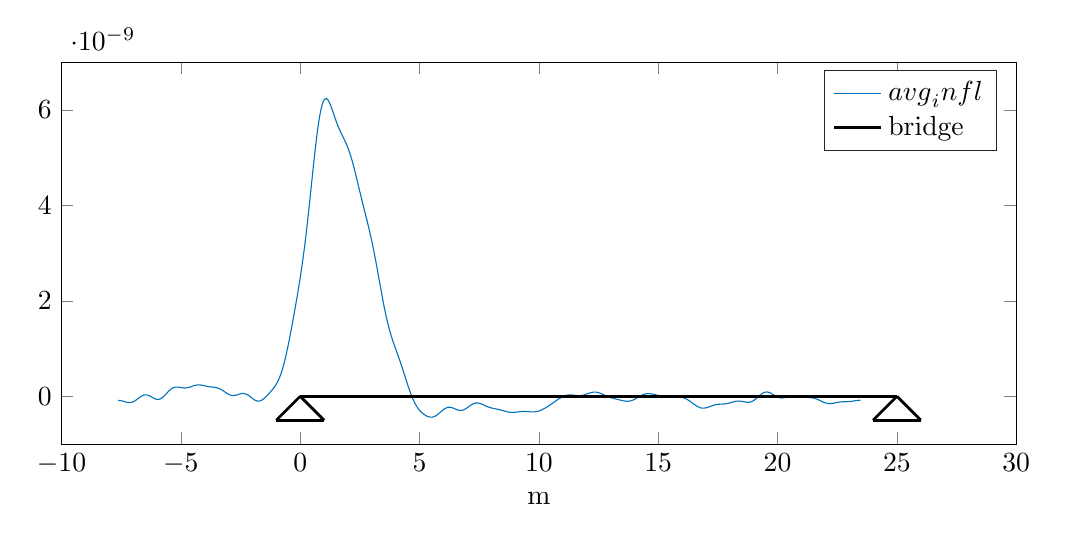
\begin{tikzpicture}

\begin{axis}[%
width=\textwidth,
height=0.4\textwidth,
at={(0\textwidth,0\textwidth)},
scale only axis,
xmin=-10,
xmax=30,
xlabel={m},
ymin=-1e-09,
ymax=7e-09,
ylabel={},
axis background/.style={fill=white},
title style={font=\bfseries},
title={},
legend style={legend cell align=left,align=left,draw=white!15!black}
]
\addplot [color=mycolor1,solid]
  table[row sep=crcr]{%
-7.62213314941406	-8.26245233523815e-11\\
-7.602024296875	-8.3343636969587e-11\\
-7.58191544433594	-8.43560075156853e-11\\
-7.56180659179687	-8.5658763215599e-11\\
-7.54169773925781	-8.72442068954951e-11\\
-7.52158888671875	-8.90997343828375e-11\\
-7.50148003417969	-9.12078276586418e-11\\
-7.48137118164062	-9.35461245937096e-11\\
-7.46126232910156	-9.60875659558239e-11\\
-7.4411534765625	-9.88006192034701e-11\\
-7.42104462402344	-1.01649577400936e-10\\
-7.40093577148437	-1.04594930417401e-10\\
-7.38082691894531	-1.07593804426535e-10\\
-7.36071806640625	-1.1060046462071e-10\\
-7.34060921386719	-1.13566875012281e-10\\
-7.32050036132812	-1.16443308229708e-10\\
-7.30039150878906	-1.19178997343916e-10\\
-7.28028265625	-1.217228209943e-10\\
-7.26017380371094	-1.24024012436799e-10\\
-7.24006495117187	-1.26032882619369e-10\\
-7.21995609863281	-1.27701547012287e-10\\
-7.19984724609375	-1.28984645689106e-10\\
-7.17973839355469	-1.29840046073769e-10\\
-7.15962954101563	-1.30229517843459e-10\\
-7.13952068847656	-1.30119369705704e-10\\
-7.1194118359375	-1.29481038150496e-10\\
-7.09930298339844	-1.28291618809883e-10\\
-7.07919413085938	-1.26534331732471e-10\\
-7.05908527832031	-1.24198912690238e-10\\
-7.03897642578125	-1.21281923569805e-10\\
-7.01886757324219	-1.17786975947435e-10\\
-6.99875872070312	-1.13724863092641e-10\\
-6.97864986816406	-1.09113596873844e-10\\
-6.958541015625	-1.03978347334009e-10\\
-6.93843216308594	-9.83512840467825e-11\\
-6.91832331054687	-9.22713197353044e-11\\
-6.89821445800781	-8.57837580172969e-11\\
-6.87810560546875	-7.89398485113795e-11\\
-6.85799675292969	-7.1796253881086e-11\\
-6.83788790039062	-6.44144346853056e-11\\
-6.81777904785156	-5.68599591278025e-11\\
-6.7976701953125	-4.9201745936013e-11\\
-6.77756134277344	-4.15112496334726e-11\\
-6.75745249023437	-3.38615983852033e-11\\
-6.73734363769531	-2.63266953772639e-11\\
-6.71723478515625	-1.89802953279911e-11\\
-6.69712593261719	-1.18950682090405e-11\\
-6.67701708007812	-5.14166257099461e-12\\
-6.65690822753906	1.21221898484255e-12\\
-6.636799375	7.10271967323992e-12\\
-6.61669052246094	1.24706914159102e-11\\
-6.59658166992187	1.72625088155184e-11\\
-6.57647281738281	2.14308228144117e-11\\
-6.55636396484375	2.49352433448023e-11\\
-6.53625511230469	2.77429411361822e-11\\
-6.51614625976563	2.98291598478376e-11\\
-6.49603740722656	3.11776308262977e-11\\
-6.4759285546875	3.17808840346434e-11\\
-6.45581970214844	3.16404500459284e-11\\
-6.43571084960938	3.0766949418568e-11\\
-6.41560199707031	2.918006725788e-11\\
-6.39549314453125	2.69084122947729e-11\\
-6.37538429199219	2.39892613587526e-11\\
-6.35527543945313	2.04681916665529e-11\\
-6.33516658691406	1.63986048683047e-11\\
-6.315057734375	1.18411482689337e-11\\
-6.29494888183594	6.86304005265526e-12\\
-6.27484002929688	1.53730666314455e-12\\
-6.25473117675781	-4.05805828768888e-12\\
-6.23462232421875	-9.84100311074393e-12\\
-6.21451347167969	-1.57263836979408e-11\\
-6.19440461914062	-2.16269735052854e-11\\
-6.17429576660156	-2.74545049721339e-11\\
-6.1541869140625	-3.31207290145343e-11\\
-6.13407806152344	-3.85384789371497e-11\\
-6.11396920898437	-4.36227249996833e-11\\
-6.09386035644531	-4.82916059520343e-11\\
-6.07375150390625	-5.24674241171499e-11\\
-6.05364265136719	-5.60775910485225e-11\\
-6.03353379882812	-5.90555114149323e-11\\
-6.01342494628906	-6.13413935599863e-11\\
-5.99331609375	-6.28829761378331e-11\\
-5.97320724121094	-6.36361613261527e-11\\
-5.95309838867187	-6.35655463482558e-11\\
-5.93298953613281	-6.26448463811283e-11\\
-5.91288068359375	-6.08572033669751e-11\\
-5.89277183105469	-5.81953767625917e-11\\
-5.87266297851563	-5.46618138326986e-11\\
-5.85255412597656	-5.02685986985894e-11\\
-5.8324452734375	-4.50372809698169e-11\\
-5.81233642089844	-3.8998586391804e-11\\
-5.79222756835938	-3.21920135140022e-11\\
-5.77211871582031	-2.46653218996488e-11\\
-5.75200986328125	-1.64739188383697e-11\\
-5.73190101074219	-7.68015286675283e-12\\
-5.71179215820312	1.64747636896208e-12\\
-5.69168330566406	1.1435181276851e-11\\
-5.671574453125	2.16048109287028e-11\\
-5.65146560058594	3.20748247437733e-11\\
-5.63135674804687	4.27613022570251e-11\\
-5.61124789550781	5.35789755425792e-11\\
-5.59113904296875	6.44422706090727e-11\\
-5.57103019042969	7.5266344018146e-11\\
-5.55092133789062	8.59681011010379e-11\\
-5.53081248535156	9.64671824591844e-11\\
-5.5107036328125	1.06686905928022e-10\\
-5.49059478027344	1.1655515185172e-10\\
-5.47048592773437	1.26005180350435e-10\\
-5.45037707519531	1.3497637024891e-10\\
-5.43026822265625	1.43414870461539e-10\\
-5.41015937011719	1.5127415587819e-10\\
-5.39005051757812	1.58515481149301e-10\\
-5.36994166503906	1.65108227208509e-10\\
-5.3498328125	1.71030136875989e-10\\
-5.32972395996094	1.76267437434186e-10\\
-5.30961510742187	1.80814849637734e-10\\
-5.28950625488281	1.8467548418891e-10\\
-5.26939740234375	1.87860628256563e-10\\
-5.24928854980469	1.90389426118479e-10\\
-5.22917969726563	1.92288459443222e-10\\
-5.20907084472656	1.93591234077736e-10\\
-5.1889619921875	1.94337581452285e-10\\
-5.16885313964844	1.94572983837564e-10\\
-5.14874428710938	1.94347833674422e-10\\
-5.12863543457031	1.93716638031094e-10\\
-5.10852658203125	1.92737179915015e-10\\
-5.08841772949219	1.91469648667133e-10\\
-5.06830887695313	1.89975751989867e-10\\
-5.04820002441406	1.88317822301636e-10\\
-5.028091171875	1.86557930070031e-10\\
-5.00798231933594	1.84757016553724e-10\\
-4.98787346679688	1.82974057984141e-10\\
-4.96776461425781	1.81265272648561e-10\\
-4.94765576171875	1.79683381605521e-10\\
-4.92754690917969	1.78276932882956e-10\\
-4.90743805664063	1.77089697992564e-10\\
-4.88732920410156	1.76160148456355e-10\\
-4.8672203515625	1.75521018800131e-10\\
-4.84711149902344	1.75198961142634e-10\\
-4.82700264648437	1.75214295117994e-10\\
-4.80689379394531	1.75580855433786e-10\\
-4.78678494140625	1.76305937908637e-10\\
-4.76667608886719	1.77390343373577e-10\\
-4.74656723632812	1.78828517381714e-10\\
-4.72645838378906	1.80608782272425e-10\\
-4.70634953125	1.82713656799611e-10\\
-4.68624067871094	1.85120257278115e-10\\
-4.66613182617187	1.87800773046388e-10\\
-4.64602297363281	1.9072300800351e-10\\
-4.62591412109375	1.93850979069755e-10\\
-4.60580526855469	1.97145561654755e-10\\
-4.58569641601563	2.00565171606858e-10\\
-4.56558756347656	2.04066472669728e-10\\
-4.5454787109375	2.07605098193589e-10\\
-4.52536985839844	2.11136375742131e-10\\
-4.50526100585937	2.14616043302713e-10\\
-4.48515215332031	2.1800094604544e-10\\
-4.46504330078125	2.21249702981368e-10\\
-4.44493444824219	2.24323333434912e-10\\
-4.42482559570312	2.27185833960985e-10\\
-4.40471674316406	2.29804697192221e-10\\
-4.384607890625	2.32151365082055e-10\\
-4.36449903808594	2.34201610100231e-10\\
-4.34439018554687	2.35935839121284e-10\\
-4.32428133300781	2.37339316005322e-10\\
-4.30417248046875	2.38402300184592e-10\\
-4.28406362792969	2.3912009991831e-10\\
-4.26395477539062	2.39493040241657e-10\\
-4.24384592285156	2.3952634699124e-10\\
-4.2237370703125	2.39229949618316e-10\\
-4.20362821777344	2.38618206781951e-10\\
-4.18351936523437	2.37709559927633e-10\\
-4.16341051269531	2.36526121184024e-10\\
-4.14330166015625	2.35093202934281e-10\\
-4.12319280761719	2.33438797323214e-10\\
-4.10308395507812	2.31593014733461e-10\\
-4.08297510253906	2.2958749089134e-10\\
-4.06286625	2.27454772736397e-10\\
-4.04275739746094	2.25227693500769e-10\\
-4.02264854492188	2.22938747590742e-10\\
-4.00253969238281	2.2061947584093e-10\\
-3.98243083984375	2.18299871522087e-10\\
-3.96232198730469	2.16007817129352e-10\\
-3.94221313476563	2.13768561464511e-10\\
-3.92210428222656	2.11604245861513e-10\\
-3.9019954296875	2.09533487599294e-10\\
-3.88188657714844	2.07571027612452e-10\\
-3.86177772460937	2.05727448563e-10\\
-3.84166887207031	2.04008968191366e-10\\
-3.82156001953125	2.02417311639995e-10\\
-3.80145116699219	2.00949665157124e-10\\
-3.78134231445312	1.99598712261677e-10\\
-3.76123346191406	1.98352752103326e-10\\
-3.741124609375	1.97195898405605e-10\\
-3.72101575683594	1.96108356055529e-10\\
-3.70090690429688	1.95066771121247e-10\\
-3.68079805175781	1.94044648859932e-10\\
-3.66068919921875	1.93012833140583e-10\\
-3.64058034667969	1.9194003966877e-10\\
-3.62047149414062	1.90793434478964e-10\\
-3.60036264160156	1.89539248369942e-10\\
-3.5802537890625	1.88143417312424e-10\\
-3.56014493652344	1.86572238366437e-10\\
-3.54003608398437	1.8479303031703e-10\\
-3.51992723144531	1.82774788076858e-10\\
-3.49981837890625	1.80488819915938e-10\\
-3.47970952636719	1.77909356763299e-10\\
-3.45960067382812	1.75014123180192e-10\\
-3.43949182128906	1.71784860125436e-10\\
-3.41938296875	1.68207790313083e-10\\
-3.39927411621094	1.64274017791266e-10\\
-3.37916526367188	1.59979854336836e-10\\
-3.35905641113281	1.55327066349095e-10\\
-3.33894755859375	1.50323037121411e-10\\
-3.31883870605469	1.44980840654113e-10\\
-3.29872985351563	1.39319224526387e-10\\
-3.27862100097656	1.33362500748684e-10\\
-3.2585121484375	1.27140344949037e-10\\
-3.23840329589844	1.20687505684888e-10\\
-3.21829444335938	1.14043427094647e-10\\
-3.19818559082031	1.07251789488096e-10\\
-3.17807673828125	1.00359973800822e-10\\
-3.15796788574219	9.34184570841012e-11\\
-3.13785903320313	8.64801473488089e-11\\
-3.11775018066406	7.95996671115611e-11\\
-3.097641328125	7.28325958871098e-11\\
-3.07753247558594	6.62346826183606e-11\\
-3.05742362304687	5.98610396218144e-11\\
-3.03731477050781	5.37653300418589e-11\\
-3.01720591796875	4.79989610444527e-11\\
-2.99709706542969	4.26102950346275e-11\\
-2.97698821289062	3.76438910506657e-11\\
-2.95687936035156	3.31397881714377e-11\\
-2.9367705078125	2.91328422757083e-11\\
-2.91666165527344	2.56521268192843e-11\\
-2.89655280273437	2.27204074566933e-11\\
-2.87644395019531	2.03536993399021e-11\\
-2.85633509765625	1.85609147913003e-11\\
-2.83622624511719	1.73436077877507e-11\\
-2.81611739257812	1.66958203248873e-11\\
-2.79600854003906	1.6604034275788e-11\\
-2.7758996875	1.70472308366547e-11\\
-2.75579083496094	1.79970580865937e-11\\
-2.73568198242188	1.94181056018713e-11\\
-2.71557312988281	2.12682834807839e-11\\
-2.69546427734375	2.34993015769769e-11\\
-2.67535542480469	2.60572432301649e-11\\
-2.65524657226563	2.88832263464359e-11\\
-2.63513771972656	3.191414333752e-11\\
-2.6150288671875	3.50834702001984e-11\\
-2.59492001464844	3.83221339223029e-11\\
-2.57481116210938	4.15594264577995e-11\\
-2.55470230957031	4.47239527351053e-11\\
-2.53459345703125	4.77445995627984e-11\\
-2.51448460449219	5.05515118852719e-11\\
-2.49437575195313	5.30770626249693e-11\\
-2.47426689941406	5.52568023321535e-11\\
-2.454158046875	5.70303750491811e-11\\
-2.43404919433594	5.83423871826145e-11\\
-2.41394034179687	5.91432167587357e-11\\
-2.39383148925781	5.93897512088408e-11\\
-2.37372263671875	5.90460427799467e-11\\
-2.35361378417969	5.80838717813065e-11\\
-2.33350493164062	5.64832091421427e-11\\
-2.31339607910156	5.42325711534727e-11\\
-2.2932872265625	5.1329260777183e-11\\
-2.27317837402344	4.77794915070155e-11\\
-2.25306952148437	4.35983914358936e-11\\
-2.23296066894531	3.88098868979725e-11\\
-2.21285181640625	3.34464667869166e-11\\
-2.19274296386719	2.75488303789637e-11\\
-2.17263411132812	2.11654231848719e-11\\
-2.15252525878906	1.43518669938065e-11\\
-2.13241640625	7.17029183024265e-12\\
-2.11230755371094	-3.11421001330563e-13\\
-2.09219870117188	-8.02047428155318e-12\\
-2.07208984863281	-1.5880056967726e-11\\
-2.05198099609375	-2.3810300311622e-11\\
-2.03187214355469	-3.17292744672136e-11\\
-2.01176329101563	-3.95540114092939e-11\\
-1.99165443847656	-4.72015395453809e-11\\
-1.9715455859375	-5.45899151763746e-11\\
-1.95143673339844	-6.16392359505443e-11\\
-1.93132788085938	-6.82726216620149e-11\\
-1.91121902832031	-7.44171481669574e-11\\
-1.89111017578125	-8.00047208232554e-11\\
-1.87100132324219	-8.49728746942414e-11\\
-1.85089247070313	-8.92654897829899e-11\\
-1.83078361816406	-9.28334107666147e-11\\
-1.810674765625	-9.56349620631533e-11\\
-1.79056591308594	-9.76363505678936e-11\\
-1.77045706054687	-9.8811950019889e-11\\
-1.75034820800781	-9.91444626797395e-11\\
-1.73023935546875	-9.86249557916465e-11\\
-1.71013050292969	-9.72527721402685e-11\\
-1.69002165039062	-9.50353158692876e-11\\
-1.66991279785156	-9.19877165764325e-11\\
-1.6498039453125	-8.81323765119292e-11\\
-1.62969509277344	-8.34984074569296e-11\\
-1.60958624023437	-7.81209655193033e-11\\
-1.58947738769531	-7.20404936313599e-11\\
-1.56936853515625	-6.53018829440686e-11\\
-1.54925968261719	-5.7953565563707e-11\\
-1.52915083007812	-5.00465521501237e-11\\
-1.50904197753906	-4.16334287742803e-11\\
-1.488933125	-3.27673281021738e-11\\
-1.46882427246094	-2.35008904217419e-11\\
-1.44871541992188	-1.38852302508767e-11\\
-1.42860656738281	-3.96892425368914e-12\\
-1.40849771484375	6.20296405252842e-12\\
-1.38838886230469	1.65898077934484e-11\\
-1.36828000976563	2.71562741328219e-11\\
-1.34817115722656	3.78731021813756e-11\\
-1.3280623046875	4.87177891578521e-11\\
-1.30795345214844	5.96751738533806e-11\\
-1.28784459960938	7.0737907934242e-11\\
-1.26773574707031	8.19068072521608e-11\\
-1.24762689453125	9.31910770923748e-11\\
-1.22751804199219	1.04608407152578e-10\\
-1.20740918945313	1.1618493398365e-10\\
-1.18730033691406	1.27955070607609e-10\\
-1.167191484375	1.39961205030485e-10\\
-1.14708263183594	1.52253271358256e-10\\
-1.12697377929687	1.64888199173127e-10\\
-1.10686492675781	1.77929248706116e-10\\
-1.08675607421875	1.91445241121789e-10\\
-1.06664722167969	2.05509694885118e-10\\
-1.04653836914062	2.20199880683247e-10\\
-1.02642951660156	2.35595808703196e-10\\
-1.0063206640625	2.51779163199164e-10\\
-0.986211811523438	2.68832200201798e-10\\
-0.966102958984375	2.86836624911323e-10\\
-0.945994106445313	3.05872465764703e-10\\
-0.92588525390625	3.26016962365414e-10\\
-0.905776401367188	3.47343484407868e-10\\
-0.885667548828125	3.69920498415789e-10\\
-0.865558696289063	3.93810598547167e-10\\
-0.84544984375	4.19069616903963e-10\\
-0.825340991210937	4.45745827732325e-10\\
-0.805232138671875	4.73879258621879e-10\\
-0.785123286132812	5.03501120327538e-10\\
-0.76501443359375	5.34633365163965e-10\\
-0.744905581054687	5.67288382084167e-10\\
-0.724796728515625	6.01468834575066e-10\\
-0.704687875976562	6.3716764541178e-10\\
-0.6845790234375	6.74368130138499e-10\\
-0.664470170898437	7.13044278917839e-10\\
-0.644361318359375	7.53161184144765e-10\\
-0.624252465820312	7.94675608987813e-10\\
-0.60414361328125	8.37536689832275e-10\\
-0.584034760742187	8.81686763489452e-10\\
-0.563925908203125	9.2706230803452e-10\\
-0.543817055664062	9.73594984273203e-10\\
-0.523708203125	1.02121276314277e-09\\
-0.503599350585938	1.06984112285218e-09\\
-0.483490498046875	1.11940429828345e-09\\
-0.463381645507813	1.16982656413187e-09\\
-0.44327279296875	1.22103353247537e-09\\
-0.423163940429688	1.27295344494559e-09\\
-0.403055087890625	1.32551843943746e-09\\
-0.382946235351563	1.37866577134525e-09\\
-0.3628373828125	1.4323389696546e-09\\
-0.342728530273438	1.48648890885018e-09\\
-0.322619677734375	1.54107477851132e-09\\
-0.302510825195313	1.59606493365436e-09\\
-0.28240197265625	1.65143761032549e-09\\
-0.262293120117188	1.70718149263583e-09\\
-0.242184267578125	1.76329611933831e-09\\
-0.222075415039062	1.81979212015117e-09\\
-0.2019665625	1.87669127430675e-09\\
-0.181857709960937	1.9340263862174e-09\\
-0.161748857421875	1.99184097567062e-09\\
-0.141640004882812	2.05018878255826e-09\\
-0.12153115234375	2.10913308877545e-09\\
-0.101422299804687	2.16874586255653e-09\\
-0.0813134472656252	2.22910673311194e-09\\
-0.0612045947265623	2.29030180595484e-09\\
-0.0410957421875002	2.35242233172348e-09\\
-0.0209868896484373	2.41556324358089e-09\\
-0.000878037109375285	2.47982158037337e-09\\
0.0192308154296876	2.54529481462385e-09\\
0.0393396679687497	2.61207910609627e-09\\
0.0594485205078126	2.68026750306783e-09\\
0.0795573730468746	2.74994811456519e-09\\
0.0996662255859375	2.82120227764035e-09\\
0.119775078125	2.89410274426723e-09\\
0.139883930664062	2.96871191262109e-09\\
0.159992783203125	3.04508012735422e-09\\
0.180101635742187	3.12324407300044e-09\\
0.20021048828125	3.20322528383248e-09\\
0.220319340820312	3.28502879236633e-09\\
0.240428193359375	3.36864193726811e-09\\
0.260537045898437	3.45403334968829e-09\\
0.2806458984375	3.5411521350442e-09\\
0.300754750976562	3.62992726502113e-09\\
0.320863603515625	3.72026719209023e-09\\
0.340972456054687	3.81205969618053e-09\\
0.36108130859375	3.90517197032547e-09\\
0.381190161132813	3.99945094916743e-09\\
0.401299013671875	4.094723881185e-09\\
0.421407866210937	4.19079914244565e-09\\
0.441516718750001	4.28746728662187e-09\\
0.461625571289063	4.38450232298094e-09\\
0.481734423828125	4.48166321110862e-09\\
0.501843276367187	4.57869555829281e-09\\
0.521952128906251	4.675333502814e-09\\
0.542060981445313	4.77130176390041e-09\\
0.562169833984375	4.86631783684034e-09\\
0.582278686523437	4.96009430973491e-09\\
0.602387539062501	5.05234127664679e-09\\
0.622496391601563	5.1427688204802e-09\\
0.642605244140625	5.23108953783412e-09\\
0.662714096679687	5.31702107731981e-09\\
0.682822949218751	5.40028866243753e-09\\
0.702931801757813	5.48062757007197e-09\\
0.723040654296875	5.55778553599395e-09\\
0.743149506835937	5.63152505944428e-09\\
0.763258359375	5.70162557991749e-09\\
0.783367211914062	5.76788550064547e-09\\
0.803476064453124	5.83012403498832e-09\\
0.823584916992188	5.8881828539501e-09\\
0.84369376953125	5.94192751532656e-09\\
0.863802622070312	5.99124865753065e-09\\
0.883911474609374	6.03606294389922e-09\\
0.904020327148438	6.07631374622406e-09\\
0.9241291796875	6.11197155933667e-09\\
0.944238032226562	6.1430341417683e-09\\
0.964346884765624	6.16952638076534e-09\\
0.984455737304688	6.19149988322179e-09\\
1.00456458984375	6.20903229735534e-09\\
1.02467344238281	6.22222637315803e-09\\
1.04478229492187	6.23120877275625e-09\\
1.06489114746094	6.2361286447788e-09\\
1.085	6.23715597961676e-09\\
1.10510885253906	6.23447976503076e-09\\
1.12521770507813	6.22830596388634e-09\\
1.14532655761719	6.21885533784752e-09\\
1.16543541015625	6.20636114260619e-09\\
1.18554426269531	6.19106672164931e-09\\
1.20565311523438	6.17322302664852e-09\\
1.22576196777344	6.15308609328612e-09\\
1.2458708203125	6.13091450169713e-09\\
1.26597967285156	6.10696685070737e-09\\
1.28608852539063	6.08149927468246e-09\\
1.30619737792969	6.05476303107805e-09\\
1.32630623046875	6.02700218570907e-09\\
1.34641508300781	5.99845142134939e-09\\
1.36652393554688	5.96933399355334e-09\\
1.38663278808594	5.93985985558016e-09\\
1.406741640625	5.91022397202904e-09\\
1.42685049316406	5.88060483828692e-09\\
1.44695934570313	5.85116322018662e-09\\
1.46706819824219	5.82204112540611e-09\\
1.48717705078125	5.79336101514806e-09\\
1.50728590332031	5.76522526156238e-09\\
1.52739475585938	5.73771585325366e-09\\
1.54750360839844	5.71089434809081e-09\\
1.5676124609375	5.68480206944943e-09\\
1.58772131347656	5.65946053900723e-09\\
1.60783016601563	5.63487213631963e-09\\
1.62793901855469	5.61102097266221e-09\\
1.64804787109375	5.58787396407446e-09\\
1.66815672363281	5.56538208620798e-09\\
1.68826557617188	5.54348179149938e-09\\
1.70837442871094	5.52209656738122e-09\\
1.72848328125	5.50113861273353e-09\\
1.74859213378906	5.48051060858217e-09\\
1.76870098632812	5.46010755818179e-09\\
1.78880983886719	5.43981867108926e-09\\
1.80891869140625	5.41952926564212e-09\\
1.82902754394531	5.39912266440637e-09\\
1.84913639648437	5.37848205764273e-09\\
1.86924524902344	5.35749231065218e-09\\
1.8893541015625	5.33604169198544e-09\\
1.90946295410156	5.31402350091994e-09\\
1.92957180664062	5.29133757429972e-09\\
1.94968065917969	5.26789165477319e-09\\
1.96978951171875	5.24360260462319e-09\\
1.98989836425781	5.21839745173087e-09\\
2.01000721679687	5.19221425671721e-09\\
2.03011606933594	5.16500279292763e-09\\
2.050224921875	5.13672503362899e-09\\
2.07033377441406	5.10735544353795e-09\\
2.09044262695312	5.07688107455559e-09\\
2.11055147949219	5.04530146830911e-09\\
2.13066033203125	5.01262837075952e-09\\
2.15076918457031	4.97888526668861e-09\\
2.17087803710937	4.94410674429575e-09\\
2.19098688964844	4.90833770238202e-09\\
2.2110957421875	4.87163241464773e-09\\
2.23120459472656	4.83405346745224e-09\\
2.25131344726562	4.79567058895883e-09\\
2.27142229980469	4.75655938889396e-09\\
2.29153115234375	4.71680002917196e-09\\
2.31164000488281	4.67647584636335e-09\\
2.33174885742187	4.63567194740865e-09\\
2.35185770996094	4.59447380009738e-09\\
2.3719665625	4.55296583964472e-09\\
2.39207541503906	4.51123011221139e-09\\
2.41218426757813	4.46934497543478e-09\\
2.43229312011719	4.42738387498581e-09\\
2.45240197265625	4.38541421485157e-09\\
2.47251082519531	4.34349633749121e-09\\
2.49261967773438	4.30168262824439e-09\\
2.51272853027344	4.26001675641485e-09\\
2.5328373828125	4.21853306333523e-09\\
2.55294623535156	4.17725610547523e-09\\
2.57305508789063	4.13620035831431e-09\\
2.59316394042969	4.0953700842984e-09\\
2.61327279296875	4.05475936577025e-09\\
2.63338164550781	4.01435230134041e-09\\
2.65349049804688	3.97412336178441e-09\\
2.67359935058594	3.93403789924496e-09\\
2.693708203125	3.89405280131767e-09\\
2.71381705566406	3.8541172795358e-09\\
2.73392590820313	3.8141737798715e-09\\
2.75403476074219	3.77415900116409e-09\\
2.77414361328125	3.73400500589259e-09\\
2.79425246582031	3.69364040644971e-09\\
2.81436131835938	3.65299160906441e-09\\
2.83447017089844	3.6119840967717e-09\\
2.8545790234375	3.57054373235144e-09\\
2.87468787597656	3.52859806195659e-09\\
2.89479672851563	3.48607760022689e-09\\
2.91490558105469	3.44291707803397e-09\\
2.93501443359375	3.39905663462034e-09\\
2.95512328613281	3.35444293676873e-09\\
2.97523213867188	3.30903020875449e-09\\
2.99534099121094	3.26278115817505e-09\\
3.01544984375	3.21566778429761e-09\\
3.03555869628906	3.16767205729352e-09\\
3.05566754882812	3.11878645861265e-09\\
3.07577640136719	3.06901437476303e-09\\
3.09588525390625	3.01837033887298e-09\\
3.11599410644531	2.96688011659251e-09\\
3.13610295898437	2.91458063510883e-09\\
3.15621181152344	2.8615197562732e-09\\
3.1763206640625	2.80775589703404e-09\\
3.19642951660156	2.75335750251166e-09\\
3.21653836914062	2.69840237910405e-09\\
3.23664722167969	2.642976896952e-09\\
3.25675607421875	2.58717507288915e-09\\
3.27686492675781	2.53109754663373e-09\\
3.29697377929687	2.47485046442132e-09\\
3.31708263183594	2.41854428551359e-09\\
3.337191484375	2.36229252803026e-09\\
3.35730033691406	2.30621047132674e-09\\
3.37740918945312	2.25041383267041e-09\\
3.39751804199219	2.19501743624643e-09\\
3.41762689453125	2.14013389254884e-09\\
3.43773574707031	2.08587230598413e-09\\
3.45784459960937	2.03233702803897e-09\\
3.47795345214844	1.97962647264834e-09\\
3.4980623046875	1.92783200945727e-09\\
3.51817115722656	1.8770369495139e-09\\
3.53828000976562	1.82731563658004e-09\\
3.55838886230469	1.77873265571995e-09\\
3.57849771484375	1.73134216914991e-09\\
3.59860656738281	1.68518738752548e-09\\
3.61871541992187	1.64030018293707e-09\\
3.63882427246094	1.59670084790361e-09\\
3.658933125	1.55439800262904e-09\\
3.67904197753906	1.51338865074388e-09\\
3.69915083007813	1.47365838172481e-09\\
3.71925968261719	1.4351817161962e-09\\
3.73936853515625	1.39792258839722e-09\\
3.75947738769531	1.3618349582728e-09\\
3.77958624023438	1.32686354394124e-09\\
3.79969509277344	1.29294466372857e-09\\
3.8198039453125	1.26000717556102e-09\\
3.83991279785156	1.22797350029e-09\\
3.86002165039063	1.19676071450506e-09\\
3.88013050292969	1.16628169758159e-09\\
3.90023935546875	1.13644631712106e-09\\
3.92034820800781	1.10716263657935e-09\\
3.94045706054688	1.07833812874585e-09\\
3.96056591308594	1.04988087883219e-09\\
3.980674765625	1.02170076125179e-09\\
4.00078361816406	9.93710574712931e-10\\
4.02089247070313	9.6582712099891e-10\\
4.04100132324219	9.37972213757015e-10\\
4.06111017578125	9.10073604747462e-10\\
4.08121902832031	8.82065816297096e-10\\
4.10132788085938	8.53890870140005e-10\\
4.12143673339844	8.25498904386776e-10\\
4.1415455859375	7.96848672022341e-10\\
4.16165443847656	7.67907916064707e-10\\
4.18176329101563	7.38653618297921e-10\\
4.20187214355469	7.09072120296284e-10\\
4.22198099609375	6.79159117257445e-10\\
4.24208984863281	6.48919526933411e-10\\
4.26219870117187	6.18367237665988e-10\\
4.28230755371094	5.8752474117247e-10\\
4.30241640625	5.56422657265794e-10\\
4.32252525878906	5.25099159109888e-10\\
4.34263411132812	4.93599308886398e-10\\
4.36274296386719	4.619743148665e-10\\
4.38285181640625	4.30280721826647e-10\\
4.40296066894531	3.98579547508047e-10\\
4.42306952148437	3.66935378387374e-10\\
4.44317837402344	3.35415438394495e-10\\
4.4632872265625	3.04088644378777e-10\\
4.48339607910156	2.73024662088422e-10\\
4.50350493164062	2.42292976190206e-10\\
4.52361378417969	2.11961987425409e-10\\
4.54372263671875	1.82098149380255e-10\\
4.56383148925781	1.52765156556664e-10\\
4.58394034179687	1.24023194475272e-10\\
4.60404919433594	9.59282614432066e-11\\
4.624158046875	6.85315703916454e-11\\
4.64426689941406	4.18790378524704e-11\\
4.66437575195312	1.6010865719997e-11\\
4.68448460449219	-9.03878004504273e-12\\
4.70459345703125	-3.32419911436412e-11\\
4.72470230957031	-5.65772380242506e-11\\
4.74481116210937	-7.90293907989802e-11\\
4.76492001464844	-1.00589641983748e-10\\
4.7850288671875	-1.21255334527322e-10\\
4.80513771972656	-1.41029699994988e-10\\
4.82524657226562	-1.59921513082371e-10\\
4.84535542480469	-1.77944669835086e-10\\
4.86546427734375	-1.951176980233e-10\\
4.88557312988281	-2.11463209052111e-10\\
4.90568198242187	-2.27007301566178e-10\\
4.92579083496094	-2.41778927519795e-10\\
4.9458996875	-2.55809231924124e-10\\
4.96600854003906	-2.69130877746089e-10\\
4.98611739257813	-2.81777367516372e-10\\
5.00622624511719	-2.93782373107018e-10\\
5.02633509765625	-3.05179084865564e-10\\
5.04644395019531	-3.15999590847713e-10\\
5.06655280273438	-3.26274296282637e-10\\
5.08666165527344	-3.36031392644454e-10\\
5.1067705078125	-3.45296384802947e-10\\
5.12687936035156	-3.5409168370106e-10\\
5.14698821289063	-3.62436270872409e-10\\
5.16709706542969	-3.70345439887269e-10\\
5.18720591796875	-3.77830618519319e-10\\
5.20731477050781	-3.84899274078268e-10\\
5.22742362304688	-3.91554902976102e-10\\
5.24753247558594	-3.97797104208424e-10\\
5.267641328125	-4.03621735058405e-10\\
5.28775018066406	-4.0902114599014e-10\\
5.30785903320313	-4.13984490411146e-10\\
5.32796788574219	-4.18498103769651e-10\\
5.34807673828125	-4.22545945329538e-10\\
5.36818559082031	-4.26110094951059e-10\\
5.38829444335938	-4.29171296313767e-10\\
5.40840329589844	-4.31709537262729e-10\\
5.4285121484375	-4.33704657351027e-10\\
5.44862100097656	-4.35136972199511e-10\\
5.46872985351563	-4.35987904005365e-10\\
5.48883870605469	-4.36240607407943e-10\\
5.50894755859375	-4.35880579965223e-10\\
5.52905641113281	-4.34896246705858e-10\\
5.54916526367187	-4.33279508596628e-10\\
5.56927411621094	-4.31026245297143e-10\\
5.58938296875	-4.28136763254472e-10\\
5.60949182128906	-4.24616181009549e-10\\
5.62960067382812	-4.20474744532006e-10\\
5.64970952636719	-4.15728066456176e-10\\
5.66981837890625	-4.10397284242367e-10\\
5.68992723144531	-4.04509133516562e-10\\
5.71003608398437	-3.98095934130158e-10\\
5.73014493652344	-3.91195487809541e-10\\
5.7502537890625	-3.83850887613631e-10\\
5.77036264160156	-3.7611024076554e-10\\
5.79047149414062	-3.68026307752244e-10\\
5.81058034667969	-3.59656061873898e-10\\
5.83068919921875	-3.51060174652838e-10\\
5.85079805175781	-3.42302433663387e-10\\
5.87090690429687	-3.33449100400156e-10\\
5.89101575683594	-3.24568216748996e-10\\
5.911124609375	-3.15728869447256e-10\\
5.93123346191406	-3.07000422606262e-10\\
5.95134231445312	-2.98451728909082e-10\\
5.97145116699219	-2.90150330482532e-10\\
5.99156001953125	-2.82161660668596e-10\\
6.01166887207031	-2.74548257983502e-10\\
6.03177772460937	-2.67369003451848e-10\\
6.05188657714844	-2.60678392239816e-10\\
6.0719954296875	-2.54525850089561e-10\\
6.09210428222656	-2.48955104482502e-10\\
6.11221313476562	-2.44003619740726e-10\\
6.13232198730469	-2.39702104423708e-10\\
6.15243083984375	-2.36074098404186e-10\\
6.17253969238281	-2.33135645926558e-10\\
6.19264854492187	-2.30895059779184e-10\\
6.21275739746094	-2.2935278046533e-10\\
6.23286625	-2.28501332954211e-10\\
6.25297510253906	-2.28325382252308e-10\\
6.27308395507813	-2.28801887675187e-10\\
6.29319280761719	-2.29900354340748e-10\\
6.31330166015625	-2.31583179065675e-10\\
6.33341051269531	-2.3380608654682e-10\\
6.35351936523438	-2.36518650466753e-10\\
6.37362821777344	-2.39664892995351e-10\\
6.3937370703125	-2.43183955083405e-10\\
6.41384592285156	-2.47010828974952e-10\\
6.43395477539063	-2.51077143515739e-10\\
6.45406362792969	-2.55311992117773e-10\\
6.47417248046875	-2.59642792663909e-10\\
6.49428133300781	-2.63996168209808e-10\\
6.51439018554688	-2.68298837068771e-10\\
6.53449903808594	-2.72478500751399e-10\\
6.554607890625	-2.76464718277725e-10\\
6.57471674316406	-2.80189755583304e-10\\
6.59482559570313	-2.83589399099237e-10\\
6.61493444824219	-2.86603723093672e-10\\
6.63504330078125	-2.8917780101119e-10\\
6.65515215332031	-2.91262351827088e-10\\
6.67526100585938	-2.92814313334209e-10\\
6.69536985839844	-2.93797335287741e-10\\
6.7154787109375	-2.94182186433432e-10\\
6.73558756347656	-2.9394707062136e-10\\
6.75569641601563	-2.93077848443691e-10\\
6.77580526855469	-2.91568162113361e-10\\
6.79591412109375	-2.89419462603085e-10\\
6.81602297363281	-2.86640939372234e-10\\
6.83613182617187	-2.83249354304783e-10\\
6.85624067871094	-2.79268782746402e-10\\
6.87634953125	-2.74730265745763e-10\\
6.89645838378906	-2.69671378757231e-10\\
6.91656723632812	-2.64135723133967e-10\\
6.93667608886719	-2.58172347717468e-10\\
6.95678494140625	-2.51835108698931e-10\\
6.97689379394531	-2.45181976678059e-10\\
6.99700264648437	-2.382743004666e-10\\
7.01711149902344	-2.31176037669277e-10\\
7.0372203515625	-2.23952962418142e-10\\
7.05732920410156	-2.16671860834193e-10\\
7.07743805664062	-2.0939972484077e-10\\
7.09754690917969	-2.02202954857346e-10\\
7.11765576171875	-1.95146581662555e-10\\
7.13776461425781	-1.88293517336238e-10\\
7.15787346679687	-1.81703844678657e-10\\
7.17798231933594	-1.75434153869138e-10\\
7.198091171875	-1.69536934376493e-10\\
7.21820002441406	-1.64060029281261e-10\\
7.23830887695312	-1.59046158228077e-10\\
7.25841772949219	-1.54532514209616e-10\\
7.27852658203125	-1.50550438306529e-10\\
7.29863543457031	-1.47125175386556e-10\\
7.31874428710937	-1.44275712616783e-10\\
7.33885313964844	-1.42014701482427e-10\\
7.3589619921875	-1.40348462850092e-10\\
7.37907084472656	-1.39277073479473e-10\\
7.39917969726562	-1.38794531290863e-10\\
7.41928854980469	-1.38888995651609e-10\\
7.43939740234375	-1.39543097967247e-10\\
7.45950625488281	-1.40734316965368e-10\\
7.47961510742187	-1.42435412254355e-10\\
7.49972395996094	-1.4461490903524e-10\\
7.5198328125	-1.47237626251967e-10\\
7.53994166503906	-1.50265239990412e-10\\
7.56005051757813	-1.53656873584851e-10\\
7.58015937011719	-1.57369705665875e-10\\
7.60026822265625	-1.61359587287395e-10\\
7.62037707519531	-1.65581659302317e-10\\
7.64048592773438	-1.69990961314432e-10\\
7.66059478027344	-1.745430238142e-10\\
7.6807036328125	-1.79194435502747e-10\\
7.70081248535156	-1.83903378314187e-10\\
7.72092133789063	-1.88630123252639e-10\\
7.74103019042969	-1.9333748085675e-10\\
7.76113904296875	-1.97991200879873e-10\\
7.78124789550781	-2.02560316615884e-10\\
7.80135674804688	-2.07017430195711e-10\\
7.82146560058594	-2.11338936114221e-10\\
7.841574453125	-2.15505181206816e-10\\
7.86168330566406	-2.19500560265605e-10\\
7.88179215820313	-2.23313547451779e-10\\
7.90190101074219	-2.26936664609719e-10\\
7.92200986328125	-2.30366388505572e-10\\
7.94211871582031	-2.33602999885443e-10\\
7.96222756835938	-2.3665037806365e-10\\
7.98233642089844	-2.39515745498323e-10\\
8.0024452734375	-2.4220936747993e-10\\
8.02255412597656	-2.4474421263906e-10\\
8.04266297851563	-2.47135580465707e-10\\
8.06277183105469	-2.49400702417293e-10\\
8.08288068359375	-2.51558323472385e-10\\
8.10298953613281	-2.53628271158847e-10\\
8.12309838867187	-2.55631019147779e-10\\
8.14320724121094	-2.5758725245874e-10\\
8.16331609375	-2.59517441169423e-10\\
8.18342494628906	-2.61441429268059e-10\\
8.20353379882813	-2.63378044934525e-10\\
8.22364265136719	-2.65344738093035e-10\\
8.24375150390625	-2.67357250553425e-10\\
8.26386035644531	-2.69429323458424e-10\\
8.28396920898437	-2.71572446090997e-10\\
8.30407806152344	-2.73795649379928e-10\\
8.3241869140625	-2.7610534668463e-10\\
8.34429576660156	-2.78505223654143e-10\\
8.36440461914063	-2.80996178152438e-10\\
8.38451347167969	-2.83576310435289e-10\\
8.40462232421875	-2.86240962965289e-10\\
8.42473117675781	-2.88982808473339e-10\\
8.44484002929688	-2.91791984128761e-10\\
8.46494888183594	-2.94656268977108e-10\\
8.485057734375	-2.97561301155182e-10\\
8.50516658691406	-3.0049083080582e-10\\
8.52527543945313	-3.03427004099229e-10\\
8.54538429199219	-3.06350673329891e-10\\
8.56549314453125	-3.09241727704302e-10\\
8.58560199707031	-3.12079439169425e-10\\
8.60571084960938	-3.14842817457832e-10\\
8.62581970214844	-3.17510968444698e-10\\
8.6459285546875	-3.20063449924215e-10\\
8.66603740722656	-3.22480619017461e-10\\
8.68614625976562	-3.24743965617478e-10\\
8.70625511230469	-3.2683642655642e-10\\
8.72636396484375	-3.28742675538715e-10\\
8.74647281738281	-3.30449384316868e-10\\
8.76658166992188	-3.31945451085305e-10\\
8.78669052246094	-3.33222192623909e-10\\
8.806799375	-3.34273497327604e-10\\
8.82690822753906	-3.35095936901342e-10\\
8.84701708007812	-3.35688835170936e-10\\
8.86712593261719	-3.36054293148498e-10\\
8.88723478515625	-3.36197170185971e-10\\
8.90734363769531	-3.36125021740513e-10\\
8.92745249023438	-3.35847994950614e-10\\
8.94756134277344	-3.35378683871381e-10\\
8.9676701953125	-3.34731946831773e-10\\
8.98777904785156	-3.3392468894627e-10\\
9.00788790039062	-3.32975613330298e-10\\
9.02799675292969	-3.31904945025144e-10\\
9.04810560546875	-3.30734132027601e-10\\
9.06821445800781	-3.29485528136783e-10\\
9.08832331054688	-3.28182062571381e-10\\
9.10843216308594	-3.268469014719e-10\\
9.128541015625	-3.25503106482699e-10\\
9.14864986816406	-3.24173295607344e-10\\
9.16875872070312	-3.2287931144882e-10\\
9.18886757324219	-3.21641901785679e-10\\
9.20897642578125	-3.2048041719949e-10\\
9.22908527832031	-3.19412530162504e-10\\
9.24919413085938	-3.18453979622792e-10\\
9.26930298339844	-3.17618344693737e-10\\
9.2894118359375	-3.16916850572996e-10\\
9.30952068847656	-3.1635820929104e-10\\
9.32962954101562	-3.15948497329735e-10\\
9.34973839355469	-3.15691071566342e-10\\
9.36984724609375	-3.15586524397222e-10\\
9.38995609863281	-3.15632678288045e-10\\
9.41006495117188	-3.15824619392989e-10\\
9.43017380371094	-3.1615476929386e-10\\
9.45028265625	-3.16612993340296e-10\\
9.47039150878906	-3.17186743533066e-10\\
9.49050036132813	-3.17861233392121e-10\\
9.51060921386719	-3.18619641796882e-10\\
9.53071806640625	-3.19443342385039e-10\\
9.55082691894531	-3.20312154753528e-10\\
9.57093577148438	-3.21204613426298e-10\\
9.59104462402344	-3.2209825034143e-10\\
9.6111534765625	-3.22969886468072e-10\\
9.63126232910156	-3.23795928092655e-10\\
9.65137118164063	-3.24552663314538e-10\\
9.67148003417969	-3.25216554362578e-10\\
9.69158888671875	-3.25764521484339e-10\\
9.71169773925781	-3.26174214365577e-10\\
9.73180659179688	-3.26424267305284e-10\\
9.75191544433594	-3.26494534695908e-10\\
9.772024296875	-3.2636630373347e-10\\
9.79213314941406	-3.26022481701599e-10\\
9.81224200195313	-3.2544775562957e-10\\
9.83235085449219	-3.24628722609613e-10\\
9.85245970703125	-3.23553989564609e-10\\
9.87256855957031	-3.22214241775505e-10\\
9.89267741210938	-3.20602279999592e-10\\
9.91278626464844	-3.18713026527693e-10\\
9.9328951171875	-3.1654350103172e-10\\
9.95300396972656	-3.14092767535995e-10\\
9.97311282226563	-3.11361854298221e-10\\
9.99322167480469	-3.08353648802034e-10\\
10.0133305273438	-3.05072770435946e-10\\
10.0334393798828	-3.01525423757537e-10\\
10.0535482324219	-2.97719235511952e-10\\
10.0736570849609	-2.93663078786121e-10\\
10.0937659375	-2.89366887831575e-10\\
10.1138747900391	-2.84841467177326e-10\\
10.1339836425781	-2.80098298679027e-10\\
10.1540924951172	-2.75149350111605e-10\\
10.1742013476563	-2.70006888811066e-10\\
10.1943102001953	-2.64683303709243e-10\\
10.2144190527344	-2.59190938886257e-10\\
10.2345279052734	-2.53541941493424e-10\\
10.2546367578125	-2.47748126579319e-10\\
10.2747456103516	-2.4182086098951e-10\\
10.2948544628906	-2.3577096811249e-10\\
10.3149633154297	-2.29608654817721e-10\\
10.3350721679688	-2.2334346148391e-10\\
10.3551810205078	-2.1698423555441e-10\\
10.3752898730469	-2.10539128590256e-10\\
10.3953987255859	-2.04015616327632e-10\\
10.415507578125	-1.97420540793762e-10\\
10.4356164306641	-1.90760173101124e-10\\
10.4557252832031	-1.84040295131977e-10\\
10.4758341357422	-1.772662979506e-10\\
10.4959429882813	-1.70443294445883e-10\\
10.5160518408203	-1.63576243417734e-10\\
10.5361606933594	-1.5667008208241e-10\\
10.5562695458984	-1.49729863788393e-10\\
10.5763783984375	-1.42760897609173e-10\\
10.5964872509766	-1.35768886414755e-10\\
10.6165961035156	-1.28760060020841e-10\\
10.6367049560547	-1.21741300074113e-10\\
10.6568138085938	-1.14720253452815e-10\\
10.6769226611328	-1.07705431142239e-10\\
10.6970315136719	-1.00706289781923e-10\\
10.7171403662109	-9.37332933715913e-11\\
10.73724921875	-8.67979529615256e-11\\
10.7573580712891	-7.99128425345174e-11\\
10.7774669238281	-7.30915897047855e-11\\
10.7975757763672	-6.63488403071998e-11\\
10.8176846289063	-5.97001964205782e-11\\
10.8377934814453	-5.31621278538265e-11\\
10.8579023339844	-4.6751857615238e-11\\
10.8780111865234	-4.04872223750846e-11\\
10.8981200390625	-3.43865094114595e-11\\
10.9182288916016	-2.84682719910366e-11\\
10.9383377441406	-2.27511255720319e-11\\
10.9584465966797	-1.72535276187412e-11\\
10.9785554492187	-1.19935441784366e-11\\
10.9986643017578	-6.98860668579537e-12\\
11.0187731542969	-2.2552627216418e-12\\
11.0388820068359	2.19107534325032e-12\\
11.058990859375	6.33637974629092e-12\\
11.0790997119141	1.01682506225276e-11\\
11.0992085644531	1.36761490239723e-11\\
11.1193174169922	1.68516155641761e-11\\
11.1394262695312	1.96884707078482e-11\\
11.1595351220703	2.21829929161135e-11\\
11.1796439746094	2.4334071112943e-11\\
11.1997528271484	2.61433282540535e-11\\
11.2198616796875	2.76152131518805e-11\\
11.2399705322266	2.87570581338683e-11\\
11.2600793847656	2.95791005802002e-11\\
11.2801882373047	3.0094466894411e-11\\
11.3002970898437	3.03191179985363e-11\\
11.3204059423828	3.02717560055802e-11\\
11.3405147949219	2.9973692297598e-11\\
11.3606236474609	2.94486778188839e-11\\
11.3807325	2.8722696971677e-11\\
11.4008413525391	2.78237270674948e-11\\
11.4209502050781	2.67814658319195e-11\\
11.4410590576172	2.56270299757083e-11\\
11.4611679101563	2.43926283224214e-11\\
11.4812767626953	2.31112134145707e-11\\
11.5013856152344	2.18161158996745e-11\\
11.5214944677734	2.05406663181644e-11\\
11.5416033203125	1.93178091714956e-11\\
11.5617121728516	1.81797143365087e-11\\
11.5818210253906	1.71573910076312e-11\\
11.6019298779297	1.62803093894567e-11\\
11.6220387304688	1.55760353273193e-11\\
11.6421475830078	1.50698829525453e-11\\
11.6622564355469	1.47845902330659e-11\\
11.6823652880859	1.47400220611624e-11\\
11.702474140625	1.49529051815601e-11\\
11.7225829931641	1.54365988691401e-11\\
11.7426918457031	1.62009048115156e-11\\
11.7628006982422	1.72519191439653e-11\\
11.7829095507813	1.85919290296564e-11\\
11.8030184033203	2.02193555847058e-11\\
11.8231272558594	2.2128744323753e-11\\
11.8432361083984	2.43108036563862e-11\\
11.8633449609375	2.67524913072309e-11\\
11.8834538134766	2.94371478723365e-11\\
11.9035626660156	3.23446760713407e-11\\
11.9236715185547	3.54517636182523e-11\\
11.9437803710938	3.873214702303e-11\\
11.9638892236328	4.21569130603665e-11\\
11.9839980761719	4.56948341098432e-11\\
12.0041069287109	4.93127330907928e-11\\
12.02421578125	5.2975873292976e-11\\
12.0443246337891	5.66483680469743e-11\\
12.0644334863281	6.02936048913579e-11\\
12.0845423388672	6.38746786817107e-11\\
12.1046511914063	6.73548279526877e-11\\
12.1247600439453	7.06978687907195e-11\\
12.1448688964844	7.38686205026848e-11\\
12.1649777490234	7.68333174746668e-11\\
12.1850866015625	7.9560001803437e-11\\
12.2051954541016	8.20188915489078e-11\\
12.2253043066406	8.41827197948772e-11\\
12.2454131591797	8.6027040113024e-11\\
12.2655220117188	8.75304944955984e-11\\
12.2856308642578	8.86750403487585e-11\\
12.3057397167969	8.94461337134955e-11\\
12.3258485693359	8.98328664962282e-11\\
12.345957421875	8.98280561375451e-11\\
12.3660662744141	8.94282868158617e-11\\
12.3861751269531	8.86339019631671e-11\\
12.4062839794922	8.74489485527994e-11\\
12.4263928320313	8.58810742942117e-11\\
12.4465016845703	8.39413795273027e-11\\
12.4666105371094	8.1644226239393e-11\\
12.4867193896484	7.90070072222522e-11\\
12.5068282421875	7.60498789360077e-11\\
12.5269370947266	7.27954621433489e-11\\
12.5470459472656	6.92685148139777e-11\\
12.5671547998047	6.54955821694253e-11\\
12.5872636523438	6.15046290368247e-11\\
12.6073725048828	5.73246599027149e-11\\
12.6274813574219	5.29853322013291e-11\\
12.6475902099609	4.85165684341144e-11\\
12.6676990625	4.39481726975603e-11\\
12.6878079150391	3.93094570954354e-11\\
12.7079167675781	3.46288833305732e-11\\
12.7280256201172	2.99337245135489e-11\\
12.7481344726563	2.52497518945939e-11\\
12.7682433251953	2.06009508262147e-11\\
12.7883521777344	1.60092698030068e-11\\
12.8084610302734	1.1494405909186e-11\\
12.8285698828125	7.0736294410973e-12\\
12.8486787353516	2.76164986982248e-12\\
12.8687875878906	-1.42947532298349e-12\\
12.8888964404297	-5.49038805525267e-12\\
12.9090052929688	-9.41443308298778e-12\\
12.9291141455078	-1.31976179132529e-11\\
12.9492229980469	-1.68385302926971e-11\\
12.9693318505859	-2.03382150086754e-11\\
12.989440703125	-2.37000123478692e-11\\
13.0095495556641	-2.6929361127998e-11\\
13.0296584082031	-3.00335697432321e-11\\
13.0497672607422	-3.30215591356645e-11\\
13.0698761132813	-3.59035820166328e-11\\
13.0899849658203	-3.86909230069205e-11\\
13.1100938183594	-4.13955846387685e-11\\
13.1302026708984	-4.40299643613661e-11\\
13.1503115234375	-4.66065278121931e-11\\
13.1704203759766	-4.91374836576194e-11\\
13.1905292285156	-5.16344652671265e-11\\
13.2106380810547	-5.41082243670771e-11\\
13.2307469335938	-5.65683416241402e-11\\
13.2508557861328	-5.90229588382829e-11\\
13.2709646386719	-6.14785370849165e-11\\
13.2910734912109	-6.39396447405539e-11\\
13.31118234375	-6.64087788623334e-11\\
13.3312911962891	-6.88862228761449e-11\\
13.3514000488281	-7.13699429685712e-11\\
13.3715089013672	-7.38555249829474e-11\\
13.3916177539063	-7.63361529985021e-11\\
13.4117266064453	-7.88026301330779e-11\\
13.4318354589844	-8.12434414639777e-11\\
13.4519443115234	-8.36448583176664e-11\\
13.4720531640625	-8.59910825470258e-11\\
13.4921620166016	-8.82644288040007e-11\\
13.5122708691406	-9.04455422349512e-11\\
13.5323797216797	-9.25136484843227e-11\\
13.5524885742187	-9.44468323975169e-11\\
13.5725974267578	-9.6222341373286e-11\\
13.5927062792969	-9.78169089360824e-11\\
13.6128151318359	-9.92070937851394e-11\\
13.632923984375	-1.00369629334144e-10\\
13.6530328369141	-1.01281778586691e-10\\
13.6731416894531	-1.01921689100633e-10\\
13.6932505419922	-1.02268742780166e-10\\
13.7133593945312	-1.02303895298083e-10\\
13.7334682470703	-1.02010000090912e-10\\
13.7535770996094	-1.01372112084489e-10\\
13.7736859521484	-1.00377766593381e-10\\
13.7937948046875	-9.90172291902138e-11\\
13.8139036572266	-9.72837127548537e-11\\
13.8340125097656	-9.51735583823329e-11\\
13.8541213623047	-9.26863773452713e-11\\
13.8742302148437	-8.98251518635257e-11\\
13.8943390673828	-8.65962930225998e-11\\
13.9144479199219	-8.3009654794129e-11\\
13.9345567724609	-7.90785037373802e-11\\
13.954665625	-7.48194445910123e-11\\
13.9747744775391	-7.0252302589831e-11\\
13.9948833300781	-6.53999639529434e-11\\
14.0149921826172	-6.02881765784185e-11\\
14.0351010351563	-5.49453135368743e-11\\
14.0552098876953	-4.94021024741345e-11\\
14.0753187402344	-4.36913245038868e-11\\
14.0954275927734	-3.78474865883365e-11\\
14.1155364453125	-3.19064717623765e-11\\
14.1356452978516	-2.59051718497755e-11\\
14.1557541503906	-1.98811075444032e-11\\
14.1758630029297	-1.38720408826022e-11\\
14.1959718554688	-7.91558521265847e-12\\
14.2160807080078	-2.0488177732248e-12\\
14.2361895605469	3.69210007519187e-12\\
14.2562984130859	9.27229006136173e-12\\
14.276407265625	1.46585069621646e-11\\
14.2965161181641	1.98194668895035e-11\\
14.3166249707031	2.47261498224519e-11\\
14.3367338232422	2.93520726944722e-11\\
14.3568426757813	3.36735297879415e-11\\
14.3769515283203	3.76697976733676e-11\\
14.3970603808594	4.13233024509908e-11\\
14.4171692333984	4.46197475999268e-11\\
14.4372780859375	4.75482013062351e-11\\
14.4573869384766	5.01011427176068e-11\\
14.4774957910156	5.22744671502021e-11\\
14.4976046435547	5.4067450843708e-11\\
14.5177134960938	5.54826764155796e-11\\
14.5378223486328	5.65259206964433e-11\\
14.5579312011719	5.72060071280636e-11\\
14.5780400537109	5.75346253658748e-11\\
14.59814890625	5.75261211434077e-11\\
14.6182577587891	5.71972598201243e-11\\
14.6383666113281	5.65669673422672e-11\\
14.6584754638672	5.56560525944161e-11\\
14.6785843164063	5.44869153043199e-11\\
14.6986931689453	5.30832437831574e-11\\
14.7188020214844	5.14697068368345e-11\\
14.7389108740234	4.96716441710238e-11\\
14.7590197265625	4.77147595345305e-11\\
14.7791285791016	4.56248207043996e-11\\
14.7992374316406	4.34273702147366e-11\\
14.8193462841797	4.11474504736783e-11\\
14.8394551367188	3.88093466040041e-11\\
14.8595639892578	3.64363499880829e-11\\
14.8796728417969	3.4050545103437e-11\\
14.8997816943359	3.16726218080951e-11\\
14.919890546875	2.93217147821838e-11\\
14.9399993994141	2.70152713616159e-11\\
14.9601082519531	2.47689485190665e-11\\
14.9802171044922	2.25965392645901e-11\\
15.0003259570313	2.05099282610912e-11\\
15.0204348095703	1.85190759861522e-11\\
15.0405436621094	1.66320303288701e-11\\
15.0606525146484	1.48549640953748e-11\\
15.0807613671875	1.31922365160797e-11\\
15.1008702197266	1.16464765073653e-11\\
15.1209790722656	1.02186851454631e-11\\
15.1410879248047	8.90835456519189e-12\\
15.1611967773438	7.71360030438689e-12\\
15.1813056298828	6.6313039789516e-12\\
15.2014144824219	5.65726309520184e-12\\
15.2215233349609	4.78634478600615e-12\\
15.2416321875	4.01264029516816e-12\\
15.2617410400391	3.32961712889734e-12\\
15.2818498925781	2.73026594219662e-12\\
15.3019587451172	2.20723942808531e-12\\
15.3220675976563	1.75298072504202e-12\\
15.3421764501953	1.35983914792137e-12\\
15.3622853027344	1.02017137448443e-12\\
15.3823941552734	7.2642657744407e-13\\
15.4025030078125	4.71214373913061e-13\\
15.4226118603516	2.47354863470317e-13\\
15.4427207128906	4.79104352423556e-14\\
15.4628295654297	-1.33800563806632e-13\\
15.4829384179688	-3.0420780042776e-13\\
15.5030472705078	-4.69509673085159e-13\\
15.5231561230469	-6.35709508112531e-13\\
15.5432649755859	-8.08665617197024e-13\\
15.563373828125	-9.94153283569528e-13\\
15.5834826806641	-1.19793646704251e-12\\
15.6035915332031	-1.4258467845599e-12\\
15.6237003857422	-1.68386713750013e-12\\
15.6438092382813	-1.97821722340554e-12\\
15.6639180908203	-2.31543809050124e-12\\
15.6840269433594	-2.70247287038656e-12\\
15.7041357958984	-3.146740858167e-12\\
15.7242446484375	-3.65620220000281e-12\\
15.7443535009766	-4.23941059433935e-12\\
15.7644623535156	-4.90555161277815e-12\\
15.7845712060547	-5.66446449659666e-12\\
15.8046800585938	-6.52664558125407e-12\\
15.8247889111328	-7.50323183908616e-12\\
15.8448977636719	-8.60596340408766e-12\\
15.8650066162109	-9.84712434607453e-12\\
15.88511546875	-1.12394613876256e-11\\
15.9052243212891	-1.27960806988827e-11\\
15.9253331738281	-1.45303233547558e-11\\
15.9454420263672	-1.64556204885833e-11\\
15.9655508789062	-1.8585329617865e-11\\
15.9856597314453	-2.09325540433528e-11\\
16.0057685839844	-2.35099476249356e-11\\
16.0258774365234	-2.63295076088531e-11\\
16.0459862890625	-2.94023585138976e-11\\
16.0660951416016	-3.27385303729536e-11\\
16.0862039941406	-3.63467348646223e-11\\
16.1063128466797	-4.02341430529182e-11\\
16.1264216992187	-4.44061685767414e-11\\
16.1465305517578	-4.88662601919613e-11\\
16.1666394042969	-5.36157075651198e-11\\
16.1867482568359	-5.86534641478404e-11\\
16.206857109375	-6.39759908248852e-11\\
16.2269659619141	-6.95771238273215e-11\\
16.2470748144531	-7.54479701375868e-11\\
16.2671836669922	-8.15768332883601e-11\\
16.2872925195312	-8.79491720763183e-11\\
16.3074013720703	-9.45475942800475e-11\\
16.3275102246094	-1.01351886994669e-10\\
16.3476190771484	-1.08339084680968e-10\\
16.3677279296875	-1.1548357548139e-10\\
16.3878367822266	-1.22757245787486e-10\\
16.4079456347656	-1.30129662461752e-10\\
16.4280544873047	-1.37568291530309e-10\\
16.4481633398437	-1.45038751580756e-10\\
16.4682721923828	-1.52505099530965e-10\\
16.4883810449219	-1.59930145888762e-10\\
16.5084898974609	-1.67275796108427e-10\\
16.52859875	-1.74503414176185e-10\\
16.5487076025391	-1.81574204131442e-10\\
16.5688164550781	-1.88449604861164e-10\\
16.5889253076172	-1.95091693197753e-10\\
16.6090341601563	-2.0146359011224e-10\\
16.6291430126953	-2.07529864629294e-10\\
16.6492518652344	-2.1325693000209e-10\\
16.6693607177734	-2.18613426676431e-10\\
16.6894695703125	-2.2357058664577e-10\\
16.7095784228516	-2.28102573952473e-10\\
16.7296872753906	-2.32186796324601e-10\\
16.7497961279297	-2.35804183249421e-10\\
16.7699049804688	-2.38939426171436e-10\\
16.7900138330078	-2.41581176959045e-10\\
16.8101226855469	-2.43722201304494e-10\\
16.8302315380859	-2.45359484299426e-10\\
16.850340390625	-2.46494286055542e-10\\
16.8704492431641	-2.47132145907757e-10\\
16.8905580957031	-2.47282834436562e-10\\
16.9106669482422	-2.46960253267045e-10\\
16.9307758007813	-2.46182283333705e-10\\
16.9508846533203	-2.44970583032194e-10\\
16.9709935058594	-2.43350338400514e-10\\
16.9911023583984	-2.41349968172153e-10\\
17.0112112109375	-2.39000787211612e-10\\
17.0313200634766	-2.36336632468288e-10\\
17.0514289160156	-2.33393456158233e-10\\
17.0715377685547	-2.30208891395518e-10\\
17.0916466210938	-2.26821795937751e-10\\
17.1117554736328	-2.23271780076172e-10\\
17.1318643261719	-2.19598724983561e-10\\
17.1519731787109	-2.15842298027743e-10\\
17.17208203125	-2.12041471660882e-10\\
17.1921908837891	-2.08234052502599e-10\\
17.2122997363281	-2.04456227146949e-10\\
17.2324085888672	-2.00742131039856e-10\\
17.2525174414063	-1.97123446496267e-10\\
17.2726262939453	-1.93629035558307e-10\\
17.2927351464844	-1.90284612941393e-10\\
17.3128439990234	-1.87112463780607e-10\\
17.3329528515625	-1.84131210281432e-10\\
17.3530617041016	-1.81355630705693e-10\\
17.3731705566406	-1.78796533394248e-10\\
17.3932794091797	-1.7646068775295e-10\\
17.4133882617188	-1.7435081331855e-10\\
17.4334971142578	-1.72465627188079e-10\\
17.4536059667969	-1.70799949250891e-10\\
17.4737148193359	-1.69344863819255e-10\\
17.493823671875	-1.6808793542355e-10\\
17.5139325244141	-1.67013475734007e-10\\
17.5340413769531	-1.66102857804725e-10\\
17.5541502294922	-1.65334873118824e-10\\
17.5742590820313	-1.6468612625716e-10\\
17.5943679345703	-1.64131461427138e-10\\
17.6144767871094	-1.6364441458209e-10\\
17.6345856396484	-1.63197684443583e-10\\
17.6546944921875	-1.62763615415737e-10\\
17.6748033447266	-1.62314685157839e-10\\
17.6949121972656	-1.61823989463326e-10\\
17.7150210498047	-1.61265717082215e-10\\
17.7351299023438	-1.60615607221442e-10\\
17.7552387548828	-1.5985138266277e-10\\
17.7753476074219	-1.58953151748883e-10\\
17.7954564599609	-1.57903772901383e-10\\
17.8155653125	-1.56689175844389e-10\\
17.8356741650391	-1.55298634307722e-10\\
17.8557830175781	-1.53724985666168e-10\\
17.8758918701172	-1.51964793726783e-10\\
17.8960007226563	-1.50018451694095e-10\\
17.9161095751953	-1.47890223212012e-10\\
17.9362184277344	-1.45588220288915e-10\\
17.9563272802734	-1.43124317845786e-10\\
17.9764361328125	-1.40514005572929e-10\\
17.9965449853516	-1.37776178725047e-10\\
18.0166538378906	-1.34932870413361e-10\\
18.0367626904297	-1.32008928853347e-10\\
18.0568715429688	-1.29031643884122e-10\\
18.0769803955078	-1.26030327877545e-10\\
18.0970892480469	-1.23035856889682e-10\\
18.1171981005859	-1.2008017856286e-10\\
18.137306953125	-1.17195793853079e-10\\
18.1574158056641	-1.14415220125825e-10\\
18.1775246582031	-1.1177044352577e-10\\
18.1976335107422	-1.09292368776219e-10\\
18.2177423632813	-1.07010274697755e-10\\
18.2378512158203	-1.04951283749518e-10\\
18.2579600683594	-1.03139853789573e-10\\
18.2780689208984	-1.01597300023341e-10\\
18.2981777734375	-1.00341354763497e-10\\
18.3182866259766	-9.9385772164758e-11\\
18.3383954785156	-9.87399845285914e-11\\
18.3585043310547	-9.84088161030315e-11\\
18.3786131835938	-9.83922595404801e-11\\
18.3987220361328	-9.86853193317152e-11\\
18.4188308886719	-9.92779256187792e-11\\
18.4389397412109	-1.00154920815579e-10\\
18.45904859375	-1.0129612044635e-10\\
18.4791574462891	-1.02676448562939e-10\\
18.4992662988281	-1.04266147036824e-10\\
18.5193751513672	-1.06031056956152e-10\\
18.5394840039062	-1.07932969307049e-10\\
18.5595928564453	-1.09930041097096e-10\\
18.5797017089844	-1.11977272102168e-10\\
18.5998105615234	-1.14027036499912e-10\\
18.6199194140625	-1.16029662807684e-10\\
18.6400282666016	-1.1793405478231e-10\\
18.6601371191406	-1.19688345275031e-10\\
18.6802459716797	-1.21240574477756e-10\\
18.7003548242187	-1.22539383554779e-10\\
18.7204636767578	-1.235347143348e-10\\
18.7405725292969	-1.24178505546663e-10\\
18.7606813818359	-1.24425376022431e-10\\
18.780790234375	-1.24233285365103e-10\\
18.8008990869141	-1.23564162785213e-10\\
18.8210079394531	-1.22384495148936e-10\\
18.8411167919922	-1.20665865746194e-10\\
18.8612256445312	-1.18385435874978e-10\\
18.8813344970703	-1.15526362040203e-10\\
18.9014433496094	-1.12078142372874e-10\\
18.9215522021484	-1.08036886777453e-10\\
18.9416610546875	-1.03405506300052e-10\\
18.9617699072266	-9.81938182642402e-11\\
18.9818787597656	-9.24185648305017e-11\\
19.0019876123047	-8.61033437844926e-11\\
19.0220964648437	-7.92784515325872e-11\\
19.0422053173828	-7.1980639464419e-11\\
19.0623141699219	-6.42527860148924e-11\\
19.0824230224609	-5.61434879061376e-11\\
19.102531875	-4.77065751569824e-11\\
19.1226407275391	-3.90005554982198e-11\\
19.1427495800781	-3.00879948113859e-11\\
19.1628584326172	-2.10348411030711e-11\\
19.1829672851563	-1.19097003232262e-11\\
19.2030761376953	-2.78307302304131e-12\\
19.2231849902344	6.27343858410385e-12\\
19.2432938427734	1.51879431546976e-11\\
19.2634026953125	2.38890820298738e-11\\
19.2835115478516	3.23068498549394e-11\\
19.3036204003906	4.03734034994158e-11\\
19.3237292529297	4.80238488893187e-11\\
19.3438381054688	5.5196995620361e-11\\
19.3639469580078	6.18360696154464e-11\\
19.3840558105469	6.78893746172422e-11\\
19.4041646630859	7.33108939596357e-11\\
19.424273515625	7.80608248318516e-11\\
19.4443823681641	8.21060381253896e-11\\
19.4644912207031	8.54204579249783e-11\\
19.4846000732422	8.79853557569861e-11\\
19.5047089257813	8.97895558279611e-11\\
19.5248177783203	9.08295486566347e-11\\
19.5449266308594	9.1109511708936e-11\\
19.5650354833984	9.0641236870491e-11\\
19.5851443359375	8.94439658180584e-11\\
19.6052531884766	8.75441355633149e-11\\
19.6253620410156	8.4975037622712e-11\\
19.6454708935547	8.17763953995484e-11\\
19.6655797460938	7.79938654332123e-11\\
19.6856885986328	7.36784691612419e-11\\
19.7057974511719	6.88859627386465e-11\\
19.7259063037109	6.36761532536105e-11\\
19.74601515625	5.8112170358457e-11\\
19.7661240087891	5.22597028902807e-11\\
19.7862328613281	4.61862104795355e-11\\
19.8063417138672	3.99601204315561e-11\\
19.8264505664063	3.36500203116653e-11\\
19.8465594189453	2.73238566676697e-11\\
19.8666682714844	2.10481501843404e-11\\
19.8867771240234	1.48872372853395e-11\\
19.9068859765625	8.90254778323649e-12\\
19.9269948291016	3.15192763395859e-12\\
19.9471036816406	-2.31098481376431e-12\\
19.9672125341797	-7.43732146094252e-12\\
19.9873213867188	-1.21834792578971e-11\\
20.0074302392578	-1.65115413918395e-11\\
20.0275390917969	-2.03896201333692e-11\\
20.0476479443359	-2.37921177118673e-11\\
20.067756796875	-2.66999027323327e-11\\
20.0878656494141	-2.91004008159865e-11\\
20.1079745019531	-3.09875993274622e-11\\
20.1280833544922	-3.23619672258908e-11\\
20.1481922070313	-3.32302922291749e-11\\
20.1683010595703	-3.36054385941029e-11\\
20.1884099121094	-3.35060298741018e-11\\
20.2085187646484	-3.29560620067206e-11\\
20.2286276171875	-3.19844529906723e-11\\
20.2487364697266	-3.06245362250297e-11\\
20.2688453222656	-2.89135052899511e-11\\
20.2889541748047	-2.68918185396615e-11\\
20.3090630273438	-2.46025723465666e-11\\
20.3291718798828	-2.20908521743804e-11\\
20.3492807324219	-1.94030708639464e-11\\
20.3693895849609	-1.65863035859067e-11\\
20.3894984375	-1.36876288493013e-11\\
20.4096072900391	-1.0753484756446e-11\\
20.4297161425781	-7.82904936566071e-12\\
20.4498249951172	-4.95765357025798e-12\\
20.4699338476563	-2.18023433196497e-12\\
20.4900427001953	4.65164571299261e-13\\
20.5101515527344	2.94383789911224e-12\\
20.5302604052734	5.22480488081692e-12\\
20.5503692578125	7.28113113722969e-12\\
20.5704781103516	9.09018299475096e-12\\
20.5905869628906	1.06338116303907e-11\\
20.6106958154297	1.18984655498055e-11\\
20.6308046679688	1.28752309762574e-11\\
20.6509135205078	1.35598008005763e-11\\
20.6710223730469	1.39523737949976e-11\\
20.6911312255859	1.40574868117482e-11\\
20.711240078125	1.38837836557041e-11\\
20.7313489306641	1.34437252253422e-11\\
20.7514577832031	1.27532463445766e-11\\
20.7715666357422	1.18313654481074e-11\\
20.7916754882813	1.06997539242693e-11\\
20.8117843408203	9.38227245306576e-12\\
20.8318931933594	7.90448209591634e-12\\
20.8520020458984	6.2931381921055e-12\\
20.8721108984375	4.57567529129922e-12\\
20.8922197509766	2.7796913999764e-12\\
20.9123286035156	9.32439742285126e-13\\
20.9324374560547	-9.39663965413124e-13\\
20.9525463085938	-2.81151104837093e-12\\
20.9726551611328	-4.65973897356028e-12\\
20.9927640136719	-6.46313331708611e-12\\
21.0128728662109	-8.20298654144892e-12\\
21.03298171875	-9.86340825486289e-12\\
21.0530905712891	-1.14315824310713e-11\\
21.0731994238281	-1.28979679382345e-11\\
21.0933082763672	-1.42564396459254e-11\\
21.1134171289062	-1.55043683358039e-11\\
21.1335259814453	-1.6642638619337e-11\\
21.1536348339844	-1.76756050500084e-11\\
21.1737436865234	-1.86109875927555e-11\\
21.1938525390625	-1.94597085649733e-11\\
21.2139613916016	-2.02356740769569e-11\\
21.2340702441406	-2.0955503861226e-11\\
21.2541790966797	-2.1638214176872e-11\\
21.2742879492187	-2.23048591948917e-11\\
21.2943968017578	-2.29781369027696e-11\\
21.3145056542969	-2.36819661018775e-11\\
21.3346145068359	-2.44410415018488e-11\\
21.354723359375	-2.52803742356423e-11\\
21.3748322119141	-2.62248253230507e-11\\
21.3949410644531	-2.72986396962619e-11\\
21.4150499169922	-2.85249883677334e-11\\
21.4351587695312	-2.99255261691101e-11\\
21.4552676220703	-3.15199722228596e-11\\
21.4753764746094	-3.33257199302374e-11\\
21.4954853271484	-3.53574827763179e-11\\
21.5155941796875	-3.76269816728419e-11\\
21.5357030322266	-4.01426788919093e-11\\
21.5558118847656	-4.29095628985201e-11\\
21.5759207373047	-4.5928987579473e-11\\
21.5960295898437	-4.919856850285e-11\\
21.6161384423828	-5.27121379397832e-11\\
21.6362472949219	-5.64597594524455e-11\\
21.6563561474609	-6.04278019137497e-11\\
21.676465	-6.45990718896311e-11\\
21.6965738525391	-6.895300239852e-11\\
21.7166827050781	-7.3465895178917e-11\\
21.7367915576172	-7.81112127585193e-11\\
21.7569004101563	-8.28599158400505e-11\\
21.7770092626953	-8.76808408118471e-11\\
21.7971181152344	-9.25411115662303e-11\\
21.8172269677734	-9.74065792753827e-11\\
21.8373358203125	-1.02242283341009e-10\\
21.8574446728516	-1.07012926407151e-10\\
21.8775535253906	-1.11683356110128e-10\\
21.8976623779297	-1.16219046138898e-10\\
21.9177712304688	-1.20586569194694e-10\\
21.9378800830078	-1.24754054570235e-10\\
21.9579889355469	-1.28691623314005e-10\\
21.9780977880859	-1.32371794300101e-10\\
21.998206640625	-1.35769854983511e-10\\
22.0183154931641	-1.38864191176983e-10\\
22.0384243457031	-1.41636570830325e-10\\
22.0585331982422	-1.44072377515866e-10\\
22.0786420507813	-1.46160790113601e-10\\
22.0987509033203	-1.47894906033896e-10\\
22.1188597558594	-1.49271806201363e-10\\
22.1389686083984	-1.50292560936676e-10\\
22.1590774609375	-1.50962176799564e-10\\
22.1791863134766	-1.51289485381296e-10\\
22.1992951660156	-1.51286975944327e-10\\
22.2194040185547	-1.50970574686029e-10\\
22.2395128710938	-1.50359374238903e-10\\
22.2596217236328	-1.49475317798054e-10\\
22.2797305761719	-1.48342842975978e-10\\
22.2998394287109	-1.4698849111341e-10\\
22.31994828125	-1.45440488313406e-10\\
22.3400571337891	-1.43728304905231e-10\\
22.3601659863281	-1.41882200378068e-10\\
22.3802748388672	-1.39932761046697e-10\\
22.4003836914063	-1.37910437818341e-10\\
22.4204925439453	-1.35845091420133e-10\\
22.4406013964844	-1.33765552319972e-10\\
22.4607102490234	-1.31699202331749e-10\\
22.4808191015625	-1.296715845426e-10\\
22.5009279541016	-1.27706047740383e-10\\
22.5210368066406	-1.2582343096093e-10\\
22.5411456591797	-1.24041793125455e-10\\
22.5612545117188	-1.22376192008782e-10\\
22.5813633642578	-1.20838515980145e-10\\
22.6014722167969	-1.19437371102683e-10\\
22.6215810693359	-1.18178025278662e-10\\
22.641689921875	-1.17062410199167e-10\\
22.6617987744141	-1.16089180913952e-10\\
22.6819076269531	-1.15253831894325e-10\\
22.7020164794922	-1.1454886753425e-10\\
22.7221253320313	-1.13964024137064e-10\\
22.7422341845703	-1.13486539581666e-10\\
22.7623430371094	-1.13101466066433e-10\\
22.7824518896484	-1.12792020604432e-10\\
22.8025607421875	-1.12539967301366e-10\\
22.8226695947266	-1.12326024898922e-10\\
22.8427784472656	-1.12130292619717e-10\\
22.8628872998047	-1.11932687013696e-10\\
22.8829961523438	-1.11713382285415e-10\\
22.9031050048828	-1.11453246481342e-10\\
22.9232138574219	-1.11134265938446e-10\\
22.9433227099609	-1.10739950540277e-10\\
22.9634315625	-1.1025571259299e-10\\
22.9835404150391	-1.09669212517835e-10\\
23.0036492675781	-1.08970665053397e-10\\
23.0237581201172	-1.08153100262998e-10\\
23.0438669726563	-1.07212574341713e-10\\
23.0639758251953	-1.06148326002785e-10\\
23.0840846777344	-1.04962875083335e-10\\
23.1041935302734	-1.03662060931009e-10\\
23.1243023828125	-1.02255019102664e-10\\
23.1444112353516	-1.00754095908402e-10\\
23.1645200878906	-9.91747013538076e-11\\
23.1846289404297	-9.75351020542015e-11\\
23.2047377929688	-9.5856156701071e-11\\
23.2248466455078	-9.41609976367284e-11\\
23.2449554980469	-9.24746630230518e-11\\
23.2650643505859	-9.08236849589196e-11\\
23.285173203125	-8.9235639694556e-11\\
23.3052820556641	-8.7738666796286e-11\\
23.3253909082031	-8.63609647203412e-11\\
23.3454997607422	-8.51302707489547e-11\\
23.3656086132813	-8.40733336172119e-11\\
23.3857174658203	-8.32153874079618e-11\\
23.4058263183594	-8.2579635409346e-11\\
23.4259351708984	-8.21867526120509e-11\\
23.4460440234375	-8.20544153699585e-11\\
23.4661528759766	-8.21968664594745e-11\\
};
\addlegendentry{$\text{avg}_\text{i}\text{nfl}$};

\addplot [color=black,solid,line width=1.0pt]
  table[row sep=crcr]{%
0	0\\
1	-5e-10\\
};
\addlegendentry{bridge};

\addplot [color=black,solid,line width=1.0pt,forget plot]
  table[row sep=crcr]{%
0	0\\
-1	-5e-10\\
};
\addplot [color=black,solid,line width=1.0pt,forget plot]
  table[row sep=crcr]{%
-1	-5e-10\\
1	-5e-10\\
};
\addplot [color=black,solid,line width=1.0pt,forget plot]
  table[row sep=crcr]{%
25	0\\
26	-5e-10\\
};
\addplot [color=black,solid,line width=1.0pt,forget plot]
  table[row sep=crcr]{%
25	0\\
24	-5e-10\\
};
\addplot [color=black,solid,line width=1.0pt,forget plot]
  table[row sep=crcr]{%
24	-5e-10\\
26	-5e-10\\
};
\addplot [color=black,solid,line width=1.0pt,forget plot]
  table[row sep=crcr]{%
0	0\\
25	0\\
};
\end{axis}
\end{tikzpicture}%

		\caption{sensor 2}
		\label{fig:sensor2_averaged}
	\end{subfigure}
	\begin{subfigure}[t]{0.3\textwidth}
		% This file was created by matlab2tikz.
%
%The latest updates can be retrieved from
%  http://www.mathworks.com/matlabcentral/fileexchange/22022-matlab2tikz-matlab2tikz
%where you can also make suggestions and rate matlab2tikz.
%
\definecolor{mycolor1}{rgb}{0.00000,0.44700,0.74100}%
%
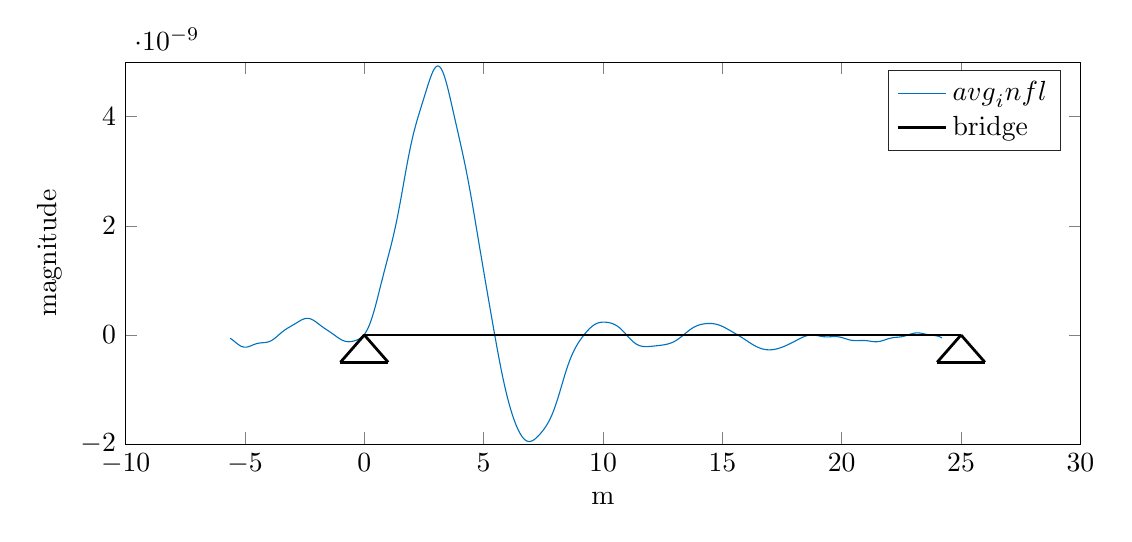
\begin{tikzpicture}

  \begin{axis}[%
    width=\textwidth,
    height=0.4\textwidth,
    at={(0\figurewidth,0\figureheight)},
    scale only axis,
    xmin=-10,
    xmax=30,
    xlabel={m},
    ymin=-2e-09,
    ymax=5e-09,
    ylabel={magnitude},
    axis background/.style={fill=white},
    title style={font=\bfseries},
    title={},
    legend style={legend cell align=left,align=left,draw=white!15!black}
    ]
    \addplot [color=mycolor1,solid]
    table[row sep=crcr]{%
    -5.62213314941406	-5.95859391362305e-11\\
    -5.602024296875	-6.5181291791226e-11\\
    -5.58191544433594	-7.10638409701917e-11\\
    -5.56180659179687	-7.72151438552805e-11\\
    -5.54169773925781	-8.36132307610648e-11\\
    -5.52158888671875	-9.02327695598874e-11\\
    -5.50148003417969	-9.70452740745131e-11\\
    -5.48137118164062	-1.04019354238107e-10\\
    -5.46126232910156	-1.11121005264341e-10\\
    -5.4411534765625	-1.18313932545766e-10\\
    -5.42104462402344	-1.25559908513947e-10\\
    -5.40093577148437	-1.32819157256502e-10\\
    -5.38082691894531	-1.40050762300414e-10\\
    -5.36071806640625	-1.47213092642858e-10\\
    -5.34060921386719	-1.54264241845138e-10\\
    -5.32050036132812	-1.61162474805724e-10\\
    -5.30039150878906	-1.67866676697901e-10\\
    -5.28028265625	-1.74336798498057e-10\\
    -5.26017380371094	-1.80534293543348e-10\\
    -5.24006495117187	-1.86422539642346e-10\\
    -5.21995609863281	-1.91967241418646e-10\\
    -5.19984724609375	-1.97136807793357e-10\\
    -5.17973839355469	-2.01902699805203e-10\\
    -5.15962954101563	-2.0623974432319e-10\\
    -5.13952068847656	-2.10126409621683e-10\\
    -5.1194118359375	-2.13545039256385e-10\\
    -5.09930298339844	-2.16482041195812e-10\\
    -5.07919413085938	-2.18928029720039e-10\\
    -5.05908527832031	-2.20877918189485e-10\\
    -5.03897642578125	-2.22330961403519e-10\\
    -5.01886757324219	-2.23290746904029e-10\\
    -4.99875872070312	-2.23765135224159e-10\\
    -4.97864986816406	-2.23766149729019e-10\\
    -4.958541015625	-2.23309817334733e-10\\
    -4.93843216308594	-2.2241596201643e-10\\
    -4.91832331054687	-2.21107953616314e-10\\
    -4.89821445800781	-2.19412415032191e-10\\
    -4.87810560546875	-2.17358891396892e-10\\
    -4.85799675292969	-2.1497948534334e-10\\
    -4.83788790039062	-2.12308462881775e-10\\
    -4.81777904785156	-2.09381834789508e-10\\
    -4.7976701953125	-2.06236918724296e-10\\
    -4.77756134277344	-2.02911887516102e-10\\
    -4.75745249023437	-1.99445309265239e-10\\
    -4.73734363769531	-1.95875684975444e-10\\
    -4.71723478515625	-1.92240989477015e-10\\
    -4.69712593261719	-1.88578221347178e-10\\
    -4.67701708007812	-1.84922967413207e-10\\
    -4.65690822753906	-1.81308987229912e-10\\
    -4.636799375	-1.77767822659487e-10\\
    -4.61669052246094	-1.74328437352008e-10\\
    -4.59658166992187	-1.71016890533163e-10\\
    -4.57647281738281	-1.67856049057565e-10\\
    -4.55636396484375	-1.6486534118685e-10\\
    -4.53625511230469	-1.62060555008563e-10\\
    -4.51614625976563	-1.59453683831591e-10\\
    -4.49603740722656	-1.57052820284307e-10\\
    -4.4759285546875	-1.54862100210779e-10\\
    -4.45581970214844	-1.52881696816613e-10\\
    -4.43571084960938	-1.5110786486778e-10\\
    -4.41560199707031	-1.49533034101702e-10\\
    -4.39549314453125	-1.48145950378352e-10\\
    -4.37538429199219	-1.46931862488631e-10\\
    -4.35527543945313	-1.45872751955644e-10\\
    -4.33516658691406	-1.4494760261959e-10\\
    -4.315057734375	-1.44132706295694e-10\\
    -4.29494888183594	-1.43402000343763e-10\\
    -4.27484002929688	-1.42727432593175e-10\\
    -4.25473117675781	-1.42079348733688e-10\\
    -4.23462232421875	-1.41426897014633e-10\\
    -4.21451347167969	-1.40738444896154e-10\\
    -4.19440461914062	-1.3998200216883e-10\\
    -4.17429576660156	-1.391256450036e-10\\
    -4.1541869140625	-1.38137935413033e-10\\
    -4.13407806152344	-1.36988330697227e-10\\
    -4.11396920898437	-1.35647577611455e-10\\
    -4.09386035644531	-1.34088086225788e-10\\
    -4.07375150390625	-1.32284278745972e-10\\
    -4.05364265136719	-1.30212908925632e-10\\
    -4.03353379882812	-1.27853348117337e-10\\
    -4.01342494628906	-1.25187834478568e-10\\
    -3.99331609375	-1.22201682361493e-10\\
    -3.97320724121094	-1.18883449465898e-10\\
    -3.95309838867187	-1.15225059914889e-10\\
    -3.93298953613281	-1.1122188201535e-10\\
    -3.91288068359375	-1.06872760081208e-10\\
    -3.89277183105469	-1.02180000319189e-10\\
    -3.87266297851563	-9.7149311395307e-11\\
    -3.85255412597656	-9.17897009075807e-11\\
    -3.8324452734375	-8.61133295782372e-11\\
    -3.81233642089844	-8.01353255389142e-11\\
    -3.79222756835938	-7.3873561607724e-11\\
    -3.77211871582031	-6.73483989404776e-11\\
    -3.75200986328125	-6.05824008732533e-11\\
    -3.73190101074219	-5.36000211544436e-11\\
    -3.71179215820312	-4.64272710859567e-11\\
    -3.69168330566406	-3.90913703517042e-11\\
    -3.671574453125	-3.1620386503041e-11\\
    -3.65146560058594	-2.40428681935748e-11\\
    -3.63135674804687	-1.63874773077974e-11\\
    -3.61124789550781	-8.68262510923966e-12\\
    -3.59113904296875	-9.56117444509251e-13\\
    -3.57103019042969	6.76518611861365e-12\\
    -3.55092133789063	1.44556945658199e-11\\
    -3.53081248535156	2.2091384758432e-11\\
    -3.5107036328125	2.96500737851831e-11\\
    -3.49059478027344	3.71116607269376e-11\\
    -3.47048592773437	4.44583346674142e-11\\
    -3.45037707519531	5.16747462746775e-11\\
    -3.43026822265625	5.8748140804963e-11\\
    -3.41015937011719	6.56684509349255e-11\\
    -3.39005051757812	7.24283484028045e-11\\
    -3.36994166503906	7.90232540253438e-11\\
    -3.3498328125	8.54513062473976e-11\\
    -3.32972395996094	9.17132889667406e-11\\
    -3.30961510742187	9.78125199496681e-11\\
    -3.28950625488281	1.03754701705475e-10\\
    -3.26939740234375	1.09547737212327e-10\\
    -3.24928854980469	1.15201513376049e-10\\
    -3.22917969726563	1.20727655550372e-10\\
    -3.20907084472656	1.26139256845926e-10\\
    -3.1889619921875	1.31450586300526e-10\\
    -3.16885313964844	1.36676780270101e-10\\
    -3.14874428710937	1.41833521624446e-10\\
    -3.12863543457031	1.46936711491547e-10\\
    -3.10852658203125	1.52002138386686e-10\\
    -3.08841772949219	1.57045149586577e-10\\
    -3.06830887695312	1.62080329564416e-10\\
    -3.04820002441406	1.6712119018956e-10\\
    -3.028091171875	1.72179877217399e-10\\
    -3.00798231933594	1.77266897353475e-10\\
    -2.98787346679687	1.82390869874589e-10\\
    -2.96776461425781	1.87558306432709e-10\\
    -2.94765576171875	1.92773422260386e-10\\
    -2.92754690917969	1.98037981544528e-10\\
    -2.90743805664063	2.03351179245545e-10\\
    -2.88732920410156	2.08709561117776e-10\\
    -2.8672203515625	2.14106983142274e-10\\
    -2.84711149902344	2.19534611022036e-10\\
    -2.82700264648437	2.24980959820647e-10\\
    -2.80689379394531	2.30431973255973e-10\\
    -2.78678494140625	2.35871141599093e-10\\
    -2.76667608886719	2.41279656582879e-10\\
    -2.74656723632812	2.46636601202286e-10\\
    -2.72645838378906	2.51919171796732e-10\\
    -2.70634953125	2.57102929350833e-10\\
    -2.68624067871094	2.62162076539505e-10\\
    -2.66613182617187	2.67069756682904e-10\\
    -2.64602297363281	2.71798370470611e-10\\
    -2.62591412109375	2.76319906067367e-10\\
    -2.60580526855469	2.8060627802771e-10\\
    -2.58569641601563	2.84629670326718e-10\\
    -2.56558756347656	2.88362878760285e-10\\
    -2.5454787109375	2.91779647981484e-10\\
    -2.52536985839844	2.94854998519591e-10\\
    -2.50526100585937	2.97565539273719e-10\\
    -2.48515215332031	2.99889761181862e-10\\
    -2.46504330078125	3.01808308035191e-10\\
    -2.44493444824219	3.03304220733073e-10\\
    -2.42482559570312	3.04363151651444e-10\\
    -2.40471674316406	3.04973546220896e-10\\
    -2.384607890625	3.05126789274601e-10\\
    -2.36449903808594	3.04817314223783e-10\\
    -2.34439018554687	3.04042673642459e-10\\
    -2.32428133300781	3.02803570386329e-10\\
    -2.30417248046875	3.01103848925172e-10\\
    -2.28406362792969	2.98950447126023e-10\\
    -2.26395477539063	2.96353309277911e-10\\
    -2.24384592285156	2.93325261690064e-10\\
    -2.2237370703125	2.89881852716632e-10\\
    -2.20362821777344	2.86041159554731e-10\\
    -2.18351936523437	2.81823564621953e-10\\
    -2.16341051269531	2.77251504738011e-10\\
    -2.14330166015625	2.72349196706808e-10\\
    -2.12319280761719	2.67142343214866e-10\\
    -2.10308395507812	2.61657823225186e-10\\
    -2.08297510253906	2.55923371248404e-10\\
    -2.06286625	2.49967250012964e-10\\
    -2.04275739746094	2.43817921130836e-10\\
    -2.02264854492188	2.3750371836413e-10\\
    -2.00253969238281	2.31052528040828e-10\\
    -1.98243083984375	2.24491481045478e-10\\
    -1.96232198730469	2.17846660625125e-10\\
    -1.94221313476563	2.11142830004543e-10\\
    -1.92210428222656	2.04403183501683e-10\\
    -1.9019954296875	1.97649124478585e-10\\
    -1.88188657714844	1.90900073059917e-10\\
    -1.86177772460937	1.84173306106803e-10\\
    -1.84166887207031	1.77483831453967e-10\\
    -1.82156001953125	1.7084429791062e-10\\
    -1.80145116699219	1.64264941997113e-10\\
    -1.78134231445312	1.57753571848032e-10\\
    -1.76123346191406	1.513155881659e-10\\
    -1.741124609375	1.44954041565867e-10\\
    -1.72101575683594	1.38669725118848e-10\\
    -1.70090690429688	1.32461300385935e-10\\
    -1.68079805175781	1.26325454748428e-10\\
    -1.66068919921875	1.20257087382392e-10\\
    -1.64058034667969	1.14249520810978e-10\\
    -1.62047149414062	1.08294734598061e-10\\
    -1.60036264160156	1.02383617428277e-10\\
    -1.5802537890625	9.65062335561872e-11\\
    -1.56014493652344	9.06520994048519e-11\\
    -1.54003608398437	8.48104659545693e-11\\
    -1.51992723144531	7.89706024881869e-11\\
    -1.49981837890625	7.31220772511519e-11\\
    -1.47970952636719	6.72550306429196e-11\\
    -1.45960067382812	6.13604366802398e-11\\
    -1.43949182128906	5.54303486610399e-11\\
    -1.41938296875	4.94581252069095e-11\\
    -1.39927411621094	4.34386331694764e-11\\
    -1.37916526367188	3.73684242464805e-11\\
    -1.35905641113281	3.12458825621759e-11\\
    -1.33894755859375	2.50713409176221e-11\\
    -1.31883870605469	1.88471639031786e-11\\
    -1.29872985351563	1.25777965806895e-11\\
    -1.27862100097656	6.26977797916739e-12\\
    -1.2585121484375	-6.82808029253862e-14\\
    -1.23840329589844	-6.42575354130434e-12\\
    -1.21829444335938	-1.27900899768774e-11\\
    -1.19818559082031	-1.91469396159261e-11\\
    -1.17807673828125	-2.54803062812779e-11\\
    -1.15796788574219	-3.17727309635696e-11\\
    -1.13785903320313	-3.80055000640254e-11\\
    -1.11775018066406	-4.41588757043082e-11\\
    -1.097641328125	-5.02123444115883e-11\\
    -1.07753247558594	-5.61448801735832e-11\\
    -1.05742362304687	-6.19352176041721e-11\\
    -1.03731477050781	-6.75621307692858e-11\\
    -1.01720591796875	-7.30047130985008e-11\\
    -0.997097065429688	-7.82426537523866e-11\\
    -0.976988212890625	-8.32565058305807e-11\\
    -0.956879360351563	-8.80279418909655e-11\\
    -0.9367705078125	-9.25399924056921e-11\\
    -0.916661655273438	-9.67772630031975e-11\\
    -0.896552802734375	-1.0072612663416e-10\\
    -0.876443950195313	-1.04374887149835e-10\\
    -0.85633509765625	-1.07713911188647e-10\\
    -0.836226245117188	-1.10735725725903e-10\\
    -0.816117392578125	-1.13435079145679e-10\\
    -0.796008540039062	-1.15808964236217e-10\\
    -0.7758996875	-1.17856602083108e-10\\
    -0.755790834960937	-1.19579386429807e-10\\
    -0.735681982421875	-1.20980788684171e-10\\
    -0.715573129882812	-1.22066224363961e-10\\
    -0.69546427734375	-1.2284288238453e-10\\
    -0.675355424804687	-1.23319519189311e-10\\
    -0.655246572265625	-1.23506220299329e-10\\
    -0.635137719726562	-1.23414132403067e-10\\
    -0.6150288671875	-1.2305516961437e-10\\
    -0.594920014648437	-1.22441697985781e-10\\
    -0.574811162109375	-1.21586202770587e-10\\
    -0.554702309570312	-1.20500943272264e-10\\
    -0.53459345703125	-1.19197600399358e-10\\
    -0.514484604492187	-1.17686922252041e-10\\
    -0.494375751953125	-1.15978373199957e-10\\
    -0.474266899414062	-1.1407979196653e-10\\
    -0.454158046875	-1.11997064210819e-10\\
    -0.434049194335937	-1.097338149937e-10\\
    -0.413940341796875	-1.07291126331005e-10\\
    -0.393831489257813	-1.04667284773809e-10\\
    -0.37372263671875	-1.01857563618153e-10\\
    -0.353613784179688	-9.8854043936779e-11\\
    -0.333504931640625	-9.56454781489381e-11\\
    -0.313396079101563	-9.22171993067314e-11\\
    -0.2932872265625	-8.85510786847002e-11\\
    -0.273178374023438	-8.46255336209009e-11\\
    -0.253069521484375	-8.04155868811338e-11\\
    -0.232960668945313	-7.58929781119401e-11\\
    -0.21285181640625	-7.10263272224508e-11\\
    -0.192742963867188	-6.5781348799448e-11\\
    -0.172634111328125	-6.01211159248688e-11\\
    -0.152525258789063	-5.40063710400729e-11\\
    -0.13241640625	-4.7395880797314e-11\\
    -0.112307553710937	-4.02468311655159e-11\\
    -0.092198701171875	-3.25152584249459e-11\\
    -0.0720898486328121	-2.41565111024254e-11\\
    -0.0519809960937501	-1.51257373746877e-11\\
    -0.0318721435546871	-5.37839200973902e-12\\
    -0.0117632910156251	5.12924346762559e-12\\
    0.00834556152343779	1.64395340037904e-11\\
    0.0284544140624998	2.85929644737838e-11\\
    0.0485632666015627	4.16276203332766e-11\\
    0.0686721191406248	5.55786824666279e-11\\
    0.0887809716796877	7.04779431749752e-11\\
    0.10888982421875	8.63533500960052e-11\\
    0.128998676757813	1.0322858460105e-10\\
    0.149107529296875	1.21122680877224e-10\\
    0.169216381835938	1.40049691476134e-10\\
    0.189325234375	1.60018404600492e-10\\
    0.209434086914063	1.81032117811935e-10\\
    0.229542939453125	2.03088472183873e-10\\
    0.249651791992187	2.26179350200669e-10\\
    0.26976064453125	2.50290839927338e-10\\
    0.289869497070312	2.75403267152228e-10\\
    0.309978349609375	3.01491296348935e-10\\
    0.330087202148437	3.28524100424268e-10\\
    0.3501960546875	3.56465598327425e-10\\
    0.370304907226562	3.85274758703788e-10\\
    0.390413759765625	4.14905966896198e-10\\
    0.410522612304687	4.45309451739552e-10\\
    0.43063146484375	4.76431767772081e-10\\
    0.450740317382812	5.08216327710516e-10\\
    0.470849169921875	5.40603979316845e-10\\
    0.490958022460938	5.73533620131889e-10\\
    0.511066875	6.06942842974724e-10\\
    0.531175727539063	6.407686046154e-10\\
    0.551284580078125	6.74947909628971e-10\\
    0.571393432617188	7.09418501137728e-10\\
    0.59150228515625	7.44119549950638e-10\\
    0.611611137695313	7.78992333518333e-10\\
    0.631719990234375	8.13980896140468e-10\\
    0.651828842773438	8.49032681991283e-10\\
    0.6719376953125	8.84099132767781e-10\\
    0.692046547851563	9.19136242111556e-10\\
    0.712155400390625	9.54105059406187e-10\\
    0.732264252929688	9.88972136102868e-10\\
    0.75237310546875	1.02370990837108e-09\\
    0.772481958007813	1.05829701060164e-09\\
    0.792590810546875	1.09271851509727e-09\\
    0.812699663085938	1.12696609416211e-09\\
    0.832808515625	1.16103810173445e-09\\
    0.852917368164062	1.19493957268639e-09\\
    0.873026220703125	1.22868213892687e-09\\
    0.893135073242187	1.26228386247821e-09\\
    0.91324392578125	1.2957689867382e-09\\
    0.933352778320312	1.32916760817612e-09\\
    0.953461630859375	1.36251527172884e-09\\
    0.973570483398437	1.39585249414905e-09\\
    0.9936793359375	1.4292242204989e-09\\
    1.01378818847656	1.46267921986634e-09\\
    1.03389704101563	1.49626942719676e-09\\
    1.05400589355469	1.53004923886769e-09\\
    1.07411474609375	1.56407477028019e-09\\
    1.09422359863281	1.59840308428675e-09\\
    1.11433245117188	1.63309139971623e-09\\
    1.13444130371094	1.66819628958315e-09\\
    1.15455015625	1.70377287877816e-09\\
    1.17465900878906	1.73987405112412e-09\\
    1.19476786132813	1.77654967564626e-09\\
    1.21487671386719	1.81384586174541e-09\\
    1.23498556640625	1.85180425268004e-09\\
    1.25509441894531	1.89046136636061e-09\\
    1.27520327148437	1.92984799194048e-09\\
    1.29531212402344	1.96998865005893e-09\\
    1.3154209765625	2.01090112386001e-09\\
    1.33552982910156	2.0525960670848e-09\\
    1.35563868164062	2.09507669462361e-09\\
    1.37574753417969	2.13833855993052e-09\\
    1.39585638671875	2.18236942265658e-09\\
    1.41596523925781	2.22714920876277e-09\\
    1.43607409179687	2.27265006424387e-09\\
    1.45618294433594	2.31883650244227e-09\\
    1.476291796875	2.36566564377248e-09\\
    1.49640064941406	2.41308754552535e-09\\
    1.51650950195313	2.46104561829254e-09\\
    1.53661835449219	2.50947712445816e-09\\
    1.55672720703125	2.55831375316264e-09\\
    1.57683605957031	2.60748226516449e-09\\
    1.59694491210938	2.65690520012301e-09\\
    1.61705376464844	2.70650163801024e-09\\
    1.6371626171875	2.75618800564413e-09\\
    1.65727146972656	2.80587891872698e-09\\
    1.67738032226563	2.85548804928098e-09\\
    1.69748917480469	2.90492900800386e-09\\
    1.71759802734375	2.95411623082668e-09\\
    1.73770687988281	3.00296585884649e-09\\
    1.75781573242188	3.05139660083128e-09\\
    1.77792458496094	3.09933056765281e-09\\
    1.7980334375	3.14669406829414e-09\\
    1.81814229003906	3.193418357499e-09\\
    1.83825114257812	3.23944032567558e-09\\
    1.85835999511719	3.28470312233118e-09\\
    1.87846884765625	3.32915670508854e-09\\
    1.89857770019531	3.37275830721091e-09\\
    1.91868655273437	3.41547281753002e-09\\
    1.93879540527344	3.45727306771751e-09\\
    1.9589042578125	3.4981400229533e-09\\
    1.97901311035156	3.53806287321081e-09\\
    1.99912196289062	3.57703902358346e-09\\
    2.01923081542969	3.61507398330591e-09\\
    2.03933966796875	3.65218115436111e-09\\
    2.05944852050781	3.68838152179532e-09\\
    2.07955737304687	3.72370324907287e-09\\
    2.09966622558594	3.75818118297489e-09\\
    2.119775078125	3.79185627366789e-09\\
    2.13988393066406	3.82477491662406e-09\\
    2.15999278320313	3.8569882240527e-09\\
    2.18010163574219	3.88855123438919e-09\\
    2.20021048828125	3.91952206917295e-09\\
    2.22031934082031	3.94996104731902e-09\\
    2.24042819335938	3.97992976734101e-09\\
    2.26053704589844	4.00949016850901e-09\\
    2.2806458984375	4.03870358221897e-09\\
    2.30075475097656	4.06762978500659e-09\\
    2.32086360351563	4.09632606465677e-09\\
    2.34097245605469	4.12484631073816e-09\\
    2.36108130859375	4.15324014063355e-09\\
    2.38119016113281	4.18155207174319e-09\\
    2.40129901367188	4.20982075001405e-09\\
    2.42140786621094	4.23807824430096e-09\\
    2.44151671875	4.26634941530195e-09\\
    2.46162557128906	4.29465136694005e-09\\
    2.48173442382812	4.32299298709806e-09\\
    2.50184327636719	4.3513745835622e-09\\
    2.52195212890625	4.37978761990909e-09\\
    2.54206098144531	4.40821455489082e-09\\
    2.56216983398437	4.43662878765023e-09\\
    2.58227868652344	4.46499470984703e-09\\
    2.6023875390625	4.49326786451111e-09\\
    2.62249639160156	4.52139521017708e-09\\
    2.64260524414062	4.54931548760934e-09\\
    2.66271409667969	4.57695968521523e-09\\
    2.68282294921875	4.60425159807894e-09\\
    2.70293180175781	4.63110847444616e-09\\
    2.72304065429687	4.65744174246082e-09\\
    2.74314950683594	4.68315780901446e-09\\
    2.763258359375	4.70815892172579e-09\\
    2.78336721191406	4.73234408433399e-09\\
    2.80347606445312	4.75561001517219e-09\\
    2.82358491699219	4.77785213789433e-09\\
    2.84369376953125	4.79896559326648e-09\\
    2.86380262207031	4.81884626060417e-09\\
    2.88391147460937	4.83739177734536e-09\\
    2.90402032714844	4.85450254529305e-09\\
    2.9241291796875	4.8700827122425e-09\\
    2.94423803222656	4.88404111802189e-09\\
    2.96434688476562	4.89629219441906e-09\\
    2.98445573730469	4.90675680903297e-09\\
    3.00456458984375	4.9153630437714e-09\\
    3.02467344238281	4.92204689950585e-09\\
    3.04478229492187	4.9267529192812e-09\\
    3.06489114746094	4.92943472345058e-09\\
    3.085	4.93005545115184e-09\\
    3.10510885253906	4.92858810364932e-09\\
    3.12521770507813	4.92501578621829e-09\\
    3.14532655761719	4.91933184643635e-09\\
    3.16543541015625	4.91153990795053e-09\\
    3.18554426269531	4.90165379999745e-09\\
    3.20565311523438	4.88969738415059e-09\\
    3.22576196777344	4.87570428094033e-09\\
    3.2458708203125	4.85971750012405e-09\\
    3.26597967285156	4.84178897946211e-09\\
    3.28608852539063	4.82197903786826e-09\\
    3.30619737792969	4.80035574973808e-09\\
    3.32630623046875	4.77699424810563e-09\\
    3.34641508300781	4.75197596502686e-09\\
    3.36652393554688	4.72538781823078e-09\\
    3.38663278808594	4.69732135360773e-09\\
    3.406741640625	4.66787185351442e-09\\
    3.42685049316406	4.63713742116221e-09\\
    3.44695934570313	4.60521805151716e-09\\
    3.46706819824219	4.57221469917602e-09\\
    3.48717705078125	4.53822835359271e-09\\
    3.50728590332031	4.50335913181703e-09\\
    3.52739475585938	4.46770539857544e-09\\
    3.54750360839844	4.43136292307716e-09\\
    3.5676124609375	4.39442408137574e-09\\
    3.58772131347656	4.35697711246237e-09\\
    3.60783016601563	4.31910543552387e-09\\
    3.62793901855469	4.28088703497399e-09\\
    3.64804787109375	4.24239391897282e-09\\
    3.66815672363281	4.20369165619828e-09\\
    3.68826557617188	4.16483899463707e-09\\
    3.70837442871094	4.12588756513361e-09\\
    3.72848328125	4.08688167138761e-09\\
    3.74859213378906	4.04785816703673e-09\\
    3.76870098632812	4.00884641941393e-09\\
    3.78880983886719	3.96986835854198e-09\\
    3.80891869140625	3.9309386089336e-09\\
    3.82902754394531	3.89206470081558e-09\\
    3.84913639648437	3.85324735650176e-09\\
    3.86924524902344	3.81448084681191e-09\\
    3.8893541015625	3.77575341168207e-09\\
    3.90946295410156	3.73704773844437e-09\\
    3.92957180664062	3.69834149067868e-09\\
    3.94968065917969	3.65960788005988e-09\\
    3.96978951171875	3.62081627324862e-09\\
    3.98989836425781	3.58193282560295e-09\\
    4.01000721679687	3.54292113332498e-09\\
    4.03011606933594	3.50374289560215e-09\\
    4.050224921875	3.4643585783544e-09\\
    4.07033377441406	3.42472807135646e-09\\
    4.09044262695312	3.38481133076219e-09\\
    4.11055147949219	3.34456899941404e-09\\
    4.13066033203125	3.30396299776583e-09\\
    4.15076918457031	3.26295707877677e-09\\
    4.17087803710937	3.22151734073928e-09\\
    4.19098688964844	3.17961269267433e-09\\
    4.2110957421875	3.13721526765613e-09\\
    4.23120459472656	3.09430078020228e-09\\
    4.25131344726562	3.05084882467544e-09\\
    4.27142229980469	3.00684311247743e-09\\
    4.29153115234375	2.96227164666405e-09\\
    4.31164000488281	2.91712683345886e-09\\
    4.33174885742187	2.87140553098466e-09\\
    4.35185770996094	2.82510903635141e-09\\
    4.3719665625	2.77824301302934e-09\\
    4.39207541503906	2.7308173611846e-09\\
    4.41218426757813	2.68284603435446e-09\\
    4.43229312011719	2.63434680647931e-09\\
    4.45240197265625	2.58534099388422e-09\\
    4.47251082519531	2.53585313730459e-09\\
    4.49261967773438	2.48591064947503e-09\\
    4.51272853027344	2.43554343414235e-09\\
    4.5328373828125	2.38478348261937e-09\\
    4.55294623535156	2.33366445416469e-09\\
    4.57305508789063	2.28222124655289e-09\\
    4.59316394042969	2.23048956319103e-09\\
    4.61327279296875	2.17850548304179e-09\\
    4.63338164550781	2.12630503943386e-09\\
    4.65349049804688	2.07392381358064e-09\\
    4.67359935058594	2.02139654829282e-09\\
    4.693708203125	1.96875678696579e-09\\
    4.71381705566406	1.91603654245478e-09\\
    4.73392590820313	1.86326599992757e-09\\
    4.75403476074219	1.81047325721369e-09\\
    4.77414361328125	1.7576841055595e-09\\
    4.79425246582031	1.70492185305939e-09\\
    4.81436131835938	1.65220719237342e-09\\
    4.83447017089844	1.59955811367119e-09\\
    4.8545790234375	1.54698986306978e-09\\
    4.87468787597656	1.49451494616912e-09\\
    4.89479672851563	1.44214317564161e-09\\
    4.91490558105469	1.38988176121161e-09\\
    4.93501443359375	1.33773543977355e-09\\
    4.95512328613281	1.28570664285288e-09\\
    4.97523213867188	1.23379569811837e-09\\
    4.99534099121094	1.18200106121374e-09\\
    5.01544984375	1.13031957379736e-09\\
    5.03555869628906	1.07874674336409e-09\\
    5.05566754882812	1.02727704017821e-09\\
    5.07577640136719	9.75904206471723e-10\\
    5.09588525390625	9.24621572961399e-10\\
    5.11599410644531	8.73422377709234e-10\\
    5.13610295898437	8.22300082395798e-10\\
    5.15621181152344	7.71248681191198e-10\\
    5.1763206640625	7.20262997592146e-10\\
    5.19642951660156	6.69338964842419e-10\\
    5.21653836914062	6.18473885862928e-10\\
    5.23664722167969	5.67666668981914e-10\\
    5.25675607421875	5.16918036169297e-10\\
    5.27686492675781	4.66230700935218e-10\\
    5.29697377929687	4.15609513544504e-10\\
    5.31708263183594	3.65061571718317e-10\\
    5.337191484375	3.14596295533854e-10\\
    5.35730033691406	2.64225465784664e-10\\
    5.37740918945312	2.13963225619612e-10\\
    5.39751804199219	1.63826045829719e-10\\
    5.41762689453125	1.13832654691098e-10\\
    5.43773574707031	6.4003933791122e-11\\
    5.45784459960937	1.43627817566306e-11\\
    5.47795345214844	-3.50660517396607e-11\\
    5.4980623046875	-8.42561589015383e-11\\
    5.51817115722656	-1.33179690496815e-10\\
    5.53828000976562	-1.81807592827035e-10\\
    5.55838886230469	-2.30109861232267e-10\\
    5.57849771484375	-2.78055806178588e-10\\
    5.59860656738281	-3.2561432783171e-10\\
    5.61871541992187	-3.72754194938502e-10\\
    5.63882427246094	-4.19444323820184e-10\\
    5.658933125	-4.65654053325428e-10\\
    5.67904197753906	-5.1135341169835e-10\\
    5.69915083007813	-5.56513371482303e-10\\
    5.71925968261719	-6.01106088803345e-10\\
    5.73936853515625	-6.45105123652823e-10\\
    5.75947738769531	-6.88485638112668e-10\\
    5.77958624023438	-7.3122456983423e-10\\
    5.79969509277344	-7.73300778486111e-10\\
    5.8198039453125	-8.14695163322296e-10\\
    5.83991279785156	-8.55390750481993e-10\\
    5.86002165039063	-8.95372749110208e-10\\
    5.88013050292969	-9.34628575875811e-10\\
    5.90023935546875	-9.73147847954359e-10\\
    5.92034820800781	-1.01092234502911e-09\\
    5.94045706054688	-1.04794594133785e-09\\
    5.96056591308594	-1.08421450924892e-09\\
    5.980674765625	-1.11972579627987e-09\\
    6.00078361816406	-1.15447927787074e-09\\
    6.02089247070313	-1.18847598858478e-09\\
    6.04100132324219	-1.22171833472772e-09\\
    6.06111017578125	-1.25420989164765e-09\\
    6.08121902832031	-1.28595518919721e-09\\
    6.10132788085938	-1.31695948900543e-09\\
    6.12143673339844	-1.34722855731557e-09\\
    6.1415455859375	-1.37676843719644e-09\\
    6.16165443847656	-1.40558522392716e-09\\
    6.18176329101563	-1.43368484728973e-09\\
    6.20187214355469	-1.46107286438105e-09\\
    6.22198099609375	-1.48775426637784e-09\\
    6.24208984863281	-1.51373330245808e-09\\
    6.26219870117187	-1.539013323803e-09\\
    6.28230755371094	-1.56359665028022e-09\\
    6.30241640625	-1.58748446204513e-09\\
    6.32252525878906	-1.61067671790003e-09\\
    6.34263411132812	-1.6331721018244e-09\\
    6.36274296386719	-1.65496799864214e-09\\
    6.38285181640625	-1.67606049932819e-09\\
    6.40296066894531	-1.69644443598562e-09\\
    6.42306952148437	-1.71611344605146e-09\\
    6.44317837402344	-1.73506006482247e-09\\
    6.4632872265625	-1.75327584493722e-09\\
    6.48339607910156	-1.77075150101615e-09\\
    6.50350493164062	-1.78747707725161e-09\\
    6.52361378417969	-1.8034421353627e-09\\
    6.54372263671875	-1.81863595998999e-09\\
    6.56383148925781	-1.83304777830804e-09\\
    6.58394034179687	-1.84666699038381e-09\\
    6.60404919433594	-1.85948340661012e-09\\
    6.624158046875	-1.87148748839855e-09\\
    6.64426689941406	-1.88267058822751e-09\\
    6.66437575195312	-1.89302518511073e-09\\
    6.68448460449219	-1.90254511157912e-09\\
    6.70459345703125	-1.91122576835528e-09\\
    6.72470230957031	-1.91906432304328e-09\\
    6.74481116210937	-1.9260598893553e-09\\
    6.76492001464844	-1.9322136836486e-09\\
    6.7850288671875	-1.9375291558473e-09\\
    6.80513771972656	-1.94201209217009e-09\\
    6.82524657226562	-1.94567068747194e-09\\
    6.84535542480469	-1.94851558543024e-09\\
    6.86546427734375	-1.9505598852572e-09\\
    6.88557312988281	-1.95181911409498e-09\\
    6.90568198242187	-1.95231116474093e-09\\
    6.92579083496094	-1.95205619885085e-09\\
    6.9458996875	-1.95107651627068e-09\\
    6.96600854003906	-1.94939639164555e-09\\
    6.98611739257813	-1.94704187994121e-09\\
    7.00622624511719	-1.94404059298082e-09\\
    7.02633509765625	-1.94042144954214e-09\\
    7.04644395019531	-1.93621440197117e-09\\
    7.06655280273438	-1.93145014264113e-09\\
    7.08666165527344	-1.92615979391552e-09\\
    7.1067705078125	-1.92037458555656e-09\\
    7.12687936035156	-1.91412552374964e-09\\
    7.14698821289063	-1.90744305608952e-09\\
    7.16709706542969	-1.90035673698946e-09\\
    7.18720591796875	-1.89289489803087e-09\\
    7.20731477050781	-1.88508432776508e-09\\
    7.22742362304688	-1.87694996541193e-09\\
    7.24753247558594	-1.86851461277155e-09\\
    7.267641328125	-1.85979866847759e-09\\
    7.28775018066406	-1.8508198884751e-09\\
    7.30785903320313	-1.84159317630591e-09\\
    7.32796788574219	-1.83213040643441e-09\\
    7.34807673828125	-1.82244028344936e-09\\
    7.36818559082031	-1.81252823953978e-09\\
    7.38829444335938	-1.80239637216956e-09\\
    7.40840329589844	-1.79204342337285e-09\\
    7.4285121484375	-1.7814648015669e-09\\
    7.44862100097656	-1.77065264623801e-09\\
    7.46872985351563	-1.75959593530637e-09\\
    7.48883870605469	-1.74828063442439e-09\\
    7.50894755859375	-1.73668988691781e-09\\
    7.52905641113281	-1.7248042425466e-09\\
    7.54916526367187	-1.7126019227508e-09\\
    7.56927411621094	-1.70005911956124e-09\\
    7.58938296875	-1.68715032490364e-09\\
    7.60949182128906	-1.67384868661281e-09\\
    7.62960067382812	-1.66012638710632e-09\\
    7.64970952636719	-1.64595504035044e-09\\
    7.66981837890625	-1.6313061024882e-09\\
    7.68992723144531	-1.61615129129476e-09\\
    7.71003608398437	-1.60046300948087e-09\\
    7.73014493652344	-1.58421476678396e-09\\
    7.7502537890625	-1.56738159576826e-09\\
    7.77036264160156	-1.54994045630242e-09\\
    7.79047149414062	-1.53187062379291e-09\\
    7.81058034667969	-1.51315405642418e-09\\
    7.83068919921875	-1.49377573688983e-09\\
    7.85079805175781	-1.47372398438868e-09\\
    7.87090690429687	-1.45299073300397e-09\\
    7.89101575683594	-1.43157177297702e-09\\
    7.911124609375	-1.40946695182381e-09\\
    7.93123346191406	-1.38668033271954e-09\\
    7.95134231445312	-1.36322030808457e-09\\
    7.97145116699219	-1.33909966684026e-09\\
    7.99156001953125	-1.3143356143572e-09\\
    8.01166887207031	-1.28894974468467e-09\\
    8.03177772460937	-1.26296796522161e-09\\
    8.05188657714844	-1.23642037455845e-09\\
    8.0719954296875	-1.20934109477851e-09\\
    8.09210428222656	-1.18176806005105e-09\\
    8.11221313476563	-1.15374276386744e-09\\
    8.13232198730469	-1.12530996776156e-09\\
    8.15243083984375	-1.09651737480937e-09\\
    8.17253969238281	-1.06741527161425e-09\\
    8.19264854492187	-1.03805614284984e-09\\
    8.21275739746094	-1.00849426274632e-09\\
    8.23286625	-9.78785268164379e-10\\
    8.25297510253906	-9.48985718102322e-10\\
    8.27308395507812	-9.19152644621965e-10\\
    8.29319280761719	-8.8934310025743e-10\\
    8.31330166015625	-8.59613706986877e-10\\
    8.33341051269531	-8.30020211800578e-10\\
    8.35351936523438	-8.00617053790523e-10\\
    8.37362821777344	-7.71456947518633e-10\\
    8.3937370703125	-7.42590487195119e-10\\
    8.41384592285156	-7.14065775918728e-10\\
    8.43395477539062	-6.85928083900422e-10\\
    8.45406362792969	-6.58219539215997e-10\\
    8.47417248046875	-6.30978854216178e-10\\
    8.49428133300781	-6.042410902706e-10\\
    8.51439018554688	-5.78037463040515e-10\\
    8.53449903808594	-5.52395189970584e-10\\
    8.554607890625	-5.27337381169164e-10\\
    8.57471674316406	-5.02882974315825e-10\\
    8.59482559570312	-4.79046713701259e-10\\
    8.61493444824219	-4.55839172975098e-10\\
    8.63504330078125	-4.33266820658073e-10\\
    8.65515215332031	-4.11332126972914e-10\\
    8.67526100585938	-3.90033710069786e-10\\
    8.69536985839844	-3.69366519272553e-10\\
    8.7154787109375	-3.49322052557391e-10\\
    8.73558756347656	-3.29888605100066e-10\\
    8.75569641601562	-3.11051545397081e-10\\
    8.77580526855469	-2.92793615182512e-10\\
    8.79591412109375	-2.75095249130022e-10\\
    8.81602297363281	-2.57934910150494e-10\\
    8.83613182617188	-2.41289435971943e-10\\
    8.85624067871094	-2.25134392620587e-10\\
    8.87634953125	-2.09444430410632e-10\\
    8.89645838378906	-1.94193638094849e-10\\
    8.91656723632812	-1.79355890927281e-10\\
    8.93667608886719	-1.64905188541355e-10\\
    8.95678494140625	-1.50815978748892e-10\\
    8.97689379394531	-1.37063463614618e-10\\
    8.99700264648438	-1.23623884453065e-10\\
    9.01711149902344	-1.10474782725902e-10\\
    9.0372203515625	-9.75952341828544e-11\\
    9.05732920410156	-8.49660539834307e-11\\
    9.07743805664062	-7.2569970953943e-11\\
    9.09754690917969	-6.03917695692645e-11\\
    9.11765576171875	-4.84183986952316e-11\\
    9.13776461425781	-3.66390465797593e-11\\
    9.15787346679688	-2.50451820324191e-11\\
    9.17798231933594	-1.36305621775391e-11\\
    9.198091171875	-2.39120759899899e-12\\
    9.21820002441406	8.67465388977e-12\\
    9.23830887695312	1.95666732247521e-11\\
    9.25841772949219	3.02824938291674e-11\\
    9.27852658203125	4.08178907881087e-11\\
    9.29863543457031	5.11669328425504e-11\\
    9.31874428710938	6.13221643297164e-11\\
    9.33885313964844	7.12748039840866e-11\\
    9.3589619921875	8.10149573456198e-11\\
    9.37907084472656	9.0531839400847e-11\\
    9.39917969726562	9.98140040092533e-11\\
    9.41928854980469	1.0884957664222e-10\\
    9.43939740234375	1.176264869844e-10\\
    9.45950625488281	1.26132698016838e-10\\
    9.47961510742187	1.34356428315833e-10\\
    9.49972395996094	1.4228636445929e-10\\
    9.5198328125	1.4991186063048e-10\\
    9.53994166503906	1.57223122744387e-10\\
    9.56005051757813	1.64211374690552e-10\\
    9.58015937011719	1.70869004584365e-10\\
    9.60026822265625	1.77189689241668e-10\\
    9.62037707519531	1.83168495434571e-10\\
    9.64048592773437	1.88801956844571e-10\\
    9.66059478027344	1.94088125997279e-10\\
    9.6807036328125	1.99026600836144e-10\\
    9.70081248535156	2.03618525965302e-10\\
    9.72092133789063	2.07866568958907e-10\\
    9.74103019042969	2.11774872491067e-10\\
    9.76113904296875	2.1534898338202e-10\\
    9.78124789550781	2.18595759977849e-10\\
    9.80135674804687	2.2152325957869e-10\\
    9.82146560058594	2.24140607900223e-10\\
    9.841574453125	2.2645785279175e-10\\
    9.86168330566406	2.28485804638574e-10\\
    9.88179215820313	2.3023586604402e-10\\
    9.90190101074219	2.31719853515723e-10\\
    9.92200986328125	2.32949813969979e-10\\
    9.94211871582031	2.33937838916633e-10\\
    9.96222756835937	2.34695879194574e-10\\
    9.98233642089844	2.35235563095075e-10\\
    10.0024452734375	2.35568020637574e-10\\
    10.0225541259766	2.35703716651712e-10\\
    10.0426629785156	2.35652295172282e-10\\
    10.0627718310547	2.35422437472745e-10\\
    10.0828806835938	2.35021735850872e-10\\
    10.1029895361328	2.34456585040326e-10\\
    10.1230983886719	2.33732092857902e-10\\
    10.1432072412109	2.32852011411946e-10\\
    10.16331609375	2.31818689897005e-10\\
    10.1834249462891	2.30633049687517e-10\\
    10.2035337988281	2.29294582123645e-10\\
    10.2236426513672	2.27801369059787e-10\\
    10.2437515039063	2.26150125925144e-10\\
    10.2638603564453	2.24336266730685e-10\\
    10.2839692089844	2.22353990151785e-10\\
    10.3040780615234	2.20196385525278e-10\\
    10.3241869140625	2.17855557327093e-10\\
    10.3442957666016	2.15322766445859e-10\\
    10.3644046191406	2.12588586341954e-10\\
    10.3845134716797	2.09643071983338e-10\\
    10.4046223242187	2.0647593928153e-10\\
    10.4247311767578	2.03076752615337e-10\\
    10.4448400292969	1.99435117927847e-10\\
    10.4649488818359	1.95540878814884e-10\\
    10.485057734375	1.91384312991111e-10\\
    10.5051665869141	1.86956326523418e-10\\
    10.5252754394531	1.82248643259551e-10\\
    10.5453842919922	1.77253986952486e-10\\
    10.5654931445312	1.71966253686321e-10\\
    10.5856019970703	1.66380672345706e-10\\
    10.6057108496094	1.60493951035987e-10\\
    10.6258197021484	1.54304407552639e-10\\
    10.6459285546875	1.47812082213423e-10\\
    10.6660374072266	1.41018831601887e-10\\
    10.6861462597656	1.33928402022891e-10\\
    10.7062551123047	1.2654648173625e-10\\
    10.7263639648437	1.18880731309668e-10\\
    10.7464728173828	1.10940791713023e-10\\
    10.7665816699219	1.02738270059013e-10\\
    10.7866905224609	9.42867031763515e-11\\
    10.806799375	8.56014994773467e-11\\
    10.8269082275391	7.66998598483514e-11\\
    10.8470170800781	6.76006785456115e-11\\
    10.8671259326172	5.83244253174543e-11\\
    10.8872347851563	4.88930101934423e-11\\
    10.9073436376953	3.93296325795578e-11\\
    10.9274524902344	2.9658616473212e-11\\
    10.9475613427734	1.99052337610974e-11\\
    10.9676701953125	1.00955176848142e-11\\
    10.9877790478516	2.56068652850982e-13\\
    11.0078879003906	-9.5861453581232e-12\\
    11.0279967529297	-1.94039915348412e-11\\
    11.0481056054688	-2.91703758087488e-11\\
    11.0682144580078	-3.88584450277149e-11\\
    11.0883233105469	-4.84417855108694e-11\\
    11.1084321630859	-5.78946158584902e-11\\
    11.128541015625	-6.71919719936009e-11\\
    11.1486498681641	-7.63098825403911e-11\\
    11.1687587207031	-8.52255327945602e-11\\
    11.1888675732422	-9.39174157098209e-11\\
    11.2089764257813	-1.02365468510471e-10\\
    11.2290852783203	-1.10551193739292e-10\\
    11.2491941308594	-1.18457763760192e-10\\
    11.2693029833984	-1.26070107952889e-10\\
    11.2894118359375	-1.33374982059504e-10\\
    11.3095206884766	-1.40361019367065e-10\\
    11.3296295410156	-1.47018763632625e-10\\
    11.3497383935547	-1.53340683875984e-10\\
    11.3698472460938	-1.59321171376037e-10\\
    11.3899560986328	-1.64956519407901e-10\\
    11.4100649511719	-1.70244886446704e-10\\
    11.4301738037109	-1.75186243737991e-10\\
    11.45028265625	-1.79782308292177e-10\\
    11.4703915087891	-1.84036462499559e-10\\
    11.4905003613281	-1.87953661681712e-10\\
    11.5106092138672	-1.91540330993592e-10\\
    11.5307180664063	-1.9480425316745e-10\\
    11.5508269189453	-1.97754448644341e-10\\
    11.5709357714844	-2.00401049671558e-10\\
    11.5910446240234	-2.02755169954653e-10\\
    11.6111534765625	-2.0482877144172e-10\\
    11.6312623291016	-2.06634529785757e-10\\
    11.6513711816406	-2.08185699979504e-10\\
    11.6714800341797	-2.09495983587504e-10\\
    11.6915888867188	-2.10579398913693e-10\\
    11.7116977392578	-2.11450155341577e-10\\
    11.7318065917969	-2.12122532969815e-10\\
    11.7519154443359	-2.12610768541011e-10\\
    11.772024296875	-2.12928948527775e-10\\
    11.7921331494141	-2.13090910100201e-10\\
    11.8122420019531	-2.13110150554781e-10\\
    11.8323508544922	-2.12999745639114e-10\\
    11.8524597070313	-2.12772277061571e-10\\
    11.8725685595703	-2.12439769332723e-10\\
    11.8926774121094	-2.12013635947828e-10\\
    11.9127862646484	-2.11504634789071e-10\\
    11.9328951171875	-2.10922832504301e-10\\
    11.9530039697266	-2.10277577507317e-10\\
    11.9731128222656	-2.09577481144864e-10\\
    11.9932216748047	-2.08830406488416e-10\\
    12.0133305273438	-2.08043464135643e-10\\
    12.0334393798828	-2.0722301434783e-10\\
    12.0535482324219	-2.06374674805858e-10\\
    12.0736570849609	-2.05503333238896e-10\\
    12.0937659375	-2.04613164166576e-10\\
    12.1138747900391	-2.03707648996866e-10\\
    12.1339836425781	-2.02789598737454e-10\\
    12.1540924951172	-2.01861178607549e-10\\
    12.1742013476563	-2.00923933878466e-10\\
    12.1943102001953	-1.99978816324078e-10\\
    12.2144190527344	-1.99026210724835e-10\\
    12.2345279052734	-1.98065960939959e-10\\
    12.2546367578125	-1.97097395140205e-10\\
    12.2747456103516	-1.96119349876296e-10\\
    12.2948544628906	-1.95130192744256e-10\\
    12.3149633154297	-1.94127843496427e-10\\
    12.3350721679688	-1.93109793534291e-10\\
    12.3551810205078	-1.9207312380451e-10\\
    12.3752898730469	-1.91014521201243e-10\\
    12.3953987255859	-1.89930293654082e-10\\
    12.415507578125	-1.88816384150582e-10\\
    12.4356164306641	-1.87668384003763e-10\\
    12.4557252832031	-1.86481545727239e-10\\
    12.4758341357422	-1.85250795922533e-10\\
    12.4959429882813	-1.83970748614069e-10\\
    12.5160518408203	-1.82635719486573e-10\\
    12.5361606933594	-1.81239741486882e-10\\
    12.5562695458984	-1.79776582247242e-10\\
    12.5763783984375	-1.78239763770197e-10\\
    12.5964872509766	-1.76622584786375e-10\\
    12.6165961035156	-1.74918146156427e-10\\
    12.6367049560547	-1.73119379637753e-10\\
    12.6568138085938	-1.71219080276353e-10\\
    12.6769226611328	-1.69209942615295e-10\\
    12.6970315136719	-1.67084600835106e-10\\
    12.7171403662109	-1.64835672859243e-10\\
    12.73724921875	-1.62455808371236e-10\\
    12.7573580712891	-1.59937740600579e-10\\
    12.7774669238281	-1.57274341643792e-10\\
    12.7975757763672	-1.54458680996793e-10\\
    12.8176846289063	-1.5148408688661e-10\\
    12.8377934814453	-1.48344209906101e-10\\
    12.8579023339844	-1.450330883765e-10\\
    12.8780111865234	-1.41545214790534e-10\\
    12.8981200390625	-1.37875602625358e-10\\
    12.9182288916016	-1.34019852760543e-10\\
    12.9383377441406	-1.29974218693392e-10\\
    12.9584465966797	-1.25735669712538e-10\\
    12.9785554492187	-1.21301951172294e-10\\
    12.9986643017578	-1.16671641004806e-10\\
    13.0187731542969	-1.11844201615463e-10\\
    13.0388820068359	-1.06820026329106e-10\\
    13.058990859375	-1.01600479590553e-10\\
    13.0790997119141	-9.61879301723524e-11\\
    13.0992085644531	-9.05857767051751e-11\\
    13.1193174169922	-8.47984649210375e-11\\
    13.1394262695312	-7.8831496085717e-11\\
    13.1595351220703	-7.26914261932494e-11\\
    13.1796439746094	-6.63858556009383e-11\\
    13.1997528271484	-5.99234088964334e-11\\
    13.2198616796875	-5.33137049076203e-11\\
    13.2399705322266	-4.6567316889562e-11\\
    13.2600793847656	-3.96957230488521e-11\\
    13.2801882373047	-3.27112476925586e-11\\
    13.3002970898437	-2.56269934146655e-11\\
    13.3204059423828	-1.84567648556308e-11\\
    13.3405147949219	-1.12149846886027e-11\\
    13.3606236474609	-3.91660259706973e-12\\
    13.3807325	3.42300188834896e-12\\
    13.4008413525391	1.07881217333124e-11\\
    13.4209502050781	1.81628288811532e-11\\
    13.4410590576172	2.55310837613013e-11\\
    13.4611679101563	3.28768466588512e-11\\
    13.4812767626953	4.01841897394396e-11\\
    13.5013856152344	4.74374084991072e-11\\
    13.5214944677734	5.46211314005988e-11\\
    13.5416033203125	6.17204264656516e-11\\
    13.5617121728516	6.87209036174597e-11\\
    13.5818210253906	7.56088116084094e-11\\
    13.6019298779297	8.23711284250052e-11\\
    13.6220387304688	8.89956441339216e-11\\
    13.6421475830078	9.54710352195421e-11\\
    13.6622564355469	1.01786929563014e-10\\
    13.6823652880859	1.07933961324547e-10\\
    13.702474140625	1.13903815112856e-10\\
    13.7225829931641	1.19689258956851e-10\\
    13.7426918457031	1.25284165732861e-10\\
    13.7628006982422	1.3068352284437e-10\\
    13.7829095507813	1.35883430098065e-10\\
    13.8030184033203	1.40881085868299e-10\\
    13.8231272558594	1.45674761789605e-10\\
    13.8432361083984	1.50263766361672e-10\\
    13.8633449609375	1.54648397991311e-10\\
    13.8834538134766	1.58829888129266e-10\\
    13.9035626660156	1.6281033528459e-10\\
    13.9236715185547	1.66592630813882e-10\\
    13.9437803710938	1.70180377485342e-10\\
    13.9638892236328	1.73577801907004e-10\\
    13.9839980761719	1.76789661983296e-10\\
    14.0041069287109	1.79821150623335e-10\\
    14.02421578125	1.82677796967068e-10\\
    14.0443246337891	1.85365366421178e-10\\
    14.0644334863281	1.87889760804937e-10\\
    14.0845423388672	1.90256919897113e-10\\
    14.1046511914063	1.92472725648365e-10\\
    14.1247600439453	1.94542910280133e-10\\
    14.1448688964844	1.96472969430963e-10\\
    14.1649777490234	1.98268081435814e-10\\
    14.1850866015625	1.99933033733855e-10\\
    14.2051954541016	2.01472157297122e-10\\
    14.2253043066406	2.02889269857428e-10\\
    14.2454131591797	2.04187628583863e-10\\
    14.2655220117188	2.0536989272971e-10\\
    14.2856308642578	2.06438096627667e-10\\
    14.3057397167969	2.07393633267677e-10\\
    14.3258485693359	2.08237248544644e-10\\
    14.345957421875	2.08969046115772e-10\\
    14.3660662744141	2.09588502661308e-10\\
    14.3861751269531	2.10094493200143e-10\\
    14.4062839794922	2.10485325975027e-10\\
    14.4263928320313	2.10758786292836e-10\\
    14.4465016845703	2.10912188585417e-10\\
    14.4666105371094	2.10942435847398e-10\\
    14.4867193896484	2.10846085510727e-10\\
    14.5068282421875	2.10619420732668e-10\\
    14.5269370947266	2.10258526005848e-10\\
    14.5470459472656	2.09759365946435e-10\\
    14.5671547998047	2.0911786608046e-10\\
    14.5872636523438	2.0832999442895e-10\\
    14.6073725048828	2.07391842690249e-10\\
    14.6274813574219	2.06299705832502e-10\\
    14.6475902099609	2.05050158940593e-10\\
    14.6676990625	2.03640130209214e-10\\
    14.6878079150391	2.02066969036529e-10\\
    14.7079167675781	2.00328508250081e-10\\
    14.7280256201172	1.98423119587041e-10\\
    14.7481344726563	1.96349761653177e-10\\
    14.7682433251953	1.94108019697615e-10\\
    14.7883521777344	1.91698136661848e-10\\
    14.8084610302734	1.89121035089778e-10\\
    14.8285698828125	1.86378329618964e-10\\
    14.8486787353516	1.83472329909792e-10\\
    14.8687875878906	1.8040603400702e-10\\
    14.8888964404297	1.77183112265083e-10\\
    14.9090052929688	1.73807882102734e-10\\
    14.9291141455078	1.70285273982218e-10\\
    14.9492229980469	1.66620789131236e-10\\
    14.9693318505859	1.6282044964097e-10\\
    14.989440703125	1.58890741678592e-10\\
    15.0095495556641	1.54838552646685e-10\\
    15.0296584082031	1.50671103203508e-10\\
    15.0497672607422	1.46395875125989e-10\\
    15.0698761132813	1.42020536050849e-10\\
    15.0899849658203	1.37552862167595e-10\\
    15.1100938183594	1.33000659960004e-10\\
    15.1302026708984	1.28371688099704e-10\\
    15.1503115234375	1.23673580586717e-10\\
    15.1704203759766	1.18913772207541e-10\\
    15.1905292285156	1.14099427341941e-10\\
    15.2106380810547	1.09237373095823e-10\\
    15.2307469335938	1.04334037670216e-10\\
    15.2508557861328	9.93953947965501e-11\\
    15.2709646386719	9.44269149773594e-11\\
    15.2910734912109	8.94335241706339e-11\\
    15.31118234375	8.44195704467885e-11\\
    15.3312911962891	7.93887990313254e-11\\
    15.3514000488281	7.43443360253439e-11\\
    15.3715089013672	6.9288680972e-11\\
    15.3916177539063	6.42237083115241e-11\\
    15.4117266064453	5.91506776424108e-11\\
    15.4318354589844	5.40702525835654e-11\\
    15.4519443115234	4.89825279134091e-11\\
    15.4720531640625	4.38870645487505e-11\\
    15.4921620166016	3.87829318203559e-11\\
    15.5122708691406	3.36687564048652e-11\\
    15.5323797216797	2.85427771855598e-11\\
    15.5524885742187	2.34029052384261e-11\\
    15.5725974267578	1.82467880761213e-11\\
    15.5927062792969	1.30718772316006e-11\\
    15.6128151318359	7.87549822584409e-12\\
    15.632923984375	2.65492194085569e-12\\
    15.6530328369141	-2.59256359004769e-12\\
    15.6731416894531	-7.86958195759458e-12\\
    15.6932505419922	-1.31785986815486e-11\\
    15.7133593945312	-1.85218539768258e-11\\
    15.7334682470703	-2.39012988669422e-11\\
    15.7535770996094	-2.93185354735489e-11\\
    15.7736859521484	-3.47747622423233e-11\\
    15.7937948046875	-4.02707247870344e-11\\
    15.8139036572266	-4.58066729464621e-11\\
    15.8340125097656	-5.13823245543799e-11\\
    15.8541213623047	-5.69968363225508e-11\\
    15.8742302148437	-6.26487821321094e-11\\
    15.8943390673828	-6.83361389214818e-11\\
    15.9144479199219	-7.40562802506524e-11\\
    15.9345567724609	-7.98059775138255e-11\\
    15.954665625	-8.55814086668974e-11\\
    15.9747744775391	-9.13781742341494e-11\\
    15.9948833300781	-9.71913202617786e-11\\
    16.0149921826172	-1.03015367795452e-10\\
    16.0351010351563	-1.08844348376561e-10\\
    16.0552098876953	-1.14671844977999e-10\\
    16.0753187402344	-1.20491037736515e-10\\
    16.0954275927734	-1.2629475378529e-10\\
    16.1155364453125	-1.32075520448512e-10\\
    16.1356452978516	-1.37825621029385e-10\\
    16.1557541503906	-1.435371524048e-10\\
    16.1758630029297	-1.49202083633648e-10\\
    16.1959718554688	-1.54812314791554e-10\\
    16.2160807080078	-1.60359735262255e-10\\
    16.2361895605469	-1.65836280744433e-10\\
    16.2562984130859	-1.71233988272006e-10\\
    16.276407265625	-1.76545048594863e-10\\
    16.2965161181641	-1.81761855324702e-10\\
    16.3166249707031	-1.86877050316205e-10\\
    16.3367338232422	-1.91883564825799e-10\\
    16.3568426757813	-1.96774656067688e-10\\
    16.3769515283203	-2.01543938868183e-10\\
    16.3970603808594	-2.06185412203324e-10\\
    16.4171692333984	-2.10693480490019e-10\\
    16.4372780859375	-2.15062969585849e-10\\
    16.4573869384766	-2.19289137536175e-10\\
    16.4774957910156	-2.23367680187697e-10\\
    16.4976046435547	-2.27294731863933e-10\\
    16.5177134960938	-2.31066861369184e-10\\
    16.5378223486328	-2.3468106365209e-10\\
    16.5579312011719	-2.38134747517135e-10\\
    16.5780400537109	-2.4142571982147e-10\\
    16.59814890625	-2.44552166634588e-10\\
    16.6182577587891	-2.47512631869173e-10\\
    16.6383666113281	-2.50305993912463e-10\\
    16.6584754638672	-2.52931440798616e-10\\
    16.6785843164063	-2.55388444463769e-10\\
    16.6986931689453	-2.57676734616932e-10\\
    16.7188020214844	-2.59796272741872e-10\\
    16.7389108740234	-2.61747226718189e-10\\
    16.7590197265625	-2.63529946514588e-10\\
    16.7791285791016	-2.65144941364515e-10\\
    16.7992374316406	-2.66592858784956e-10\\
    16.8193462841797	-2.67874465744136e-10\\
    16.8394551367188	-2.68990632224284e-10\\
    16.8595639892578	-2.69942317362732e-10\\
    16.8796728417969	-2.70730558289498e-10\\
    16.8997816943359	-2.7135646171366e-10\\
    16.919890546875	-2.71821198245123e-10\\
    16.9399993994141	-2.72125999374577e-10\\
    16.9601082519531	-2.72272156973226e-10\\
    16.9802171044922	-2.72261025116795e-10\\
    17.0003259570313	-2.72094023986231e-10\\
    17.0204348095703	-2.7177264555151e-10\\
    17.0405436621094	-2.71298460705844e-10\\
    17.0606525146484	-2.7067312748613e-10\\
    17.0807613671875	-2.69898399992273e-10\\
    17.1008702197266	-2.68976137603558e-10\\
    17.1209790722656	-2.67908314084635e-10\\
    17.1410879248047	-2.66697026177434e-10\\
    17.1611967773438	-2.65344501287791e-10\\
    17.1813056298828	-2.63853103897239e-10\\
    17.2014144824219	-2.62225340360256e-10\\
    17.2215233349609	-2.60463861785191e-10\\
    17.2416321875	-2.58571464742174e-10\\
    17.2617410400391	-2.56551089592773e-10\\
    17.2818498925781	-2.54405816293097e-10\\
    17.3019587451172	-2.52138857583275e-10\\
    17.3220675976563	-2.4975354954066e-10\\
    17.3421764501953	-2.47253339540541e-10\\
    17.3622853027344	-2.446417717351e-10\\
    17.3823941552734	-2.41922470227787e-10\\
    17.4025030078125	-2.39099120184575e-10\\
    17.4226118603516	-2.3617544718469e-10\\
    17.4427207128906	-2.33155195169791e-10\\
    17.4628295654297	-2.30042103401307e-10\\
    17.4829384179688	-2.26839882879368e-10\\
    17.5030472705078	-2.23552192712565e-10\\
    17.5231561230469	-2.20182616954753e-10\\
    17.5432649755859	-2.16734642442474e-10\\
    17.563373828125	-2.13211638173772e-10\\
    17.5834826806641	-2.09616836765736e-10\\
    17.6035915332031	-2.05953318513818e-10\\
    17.6237003857422	-2.02223998550751e-10\\
    17.6438092382813	-1.98431617566938e-10\\
    17.6639180908203	-1.94578736507714e-10\\
    17.6840269433594	-1.90667735606543e-10\\
    17.7041357958984	-1.86700818047632e-10\\
    17.7242446484375	-1.82680018477527e-10\\
    17.7443535009766	-1.78607216504097e-10\\
    17.7644623535156	-1.74484155234061e-10\\
    17.7845712060547	-1.70312464808271e-10\\
    17.8046800585938	-1.6609369079871e-10\\
    17.8247889111328	-1.61829327234305e-10\\
    17.8448977636719	-1.57520853925604e-10\\
    17.8650066162109	-1.53169777662995e-10\\
    17.88511546875	-1.48777676771018e-10\\
    17.9052243212891	-1.44346248414174e-10\\
    17.9253331738281	-1.39877357969056e-10\\
    17.9454420263672	-1.35373089705346e-10\\
    17.9655508789062	-1.30835797955434e-10\\
    17.9856597314453	-1.2626815790092e-10\\
    18.0057685839844	-1.21673215064796e-10\\
    18.0258774365234	-1.17054432572202e-10\\
    18.0459862890625	-1.12415735230838e-10\\
    18.0660951416016	-1.07761549485262e-10\\
    18.0862039941406	-1.03096838317815e-10\\
    18.1063128466797	-9.84271302029887e-11\\
    18.1264216992187	-9.3758541271675e-11\\
    18.1465305517578	-8.90977899067775e-11\\
    18.1666394042969	-8.4452203071293e-11\\
    18.1867482568359	-7.98297137638833e-11\\
    18.206857109375	-7.52388491037039e-11\\
    18.2269659619141	-7.06887086649604e-11\\
    18.2470748144531	-6.61889328106656e-11\\
    18.2671836669922	-6.17496609128692e-11\\
    18.2872925195312	-5.73814794912838e-11\\
    18.3074013720703	-5.30953604519051e-11\\
    18.3275102246094	-4.89025897596829e-11\\
    18.3476190771484	-4.48146870324557e-11\\
    18.3677279296875	-4.08433166948336e-11\\
    18.3878367822266	-3.70001914783601e-11\\
    18.4079456347656	-3.32969691955838e-11\\
    18.4280544873047	-2.97451438485808e-11\\
    18.4481633398437	-2.63559322545905e-11\\
    18.4682721923828	-2.31401574808062e-11\\
    18.4883810449219	-2.01081304749214e-11\\
    18.5084898974609	-1.72695313560784e-11\\
    18.52859875	-1.46332918906481e-11\\
    18.5487076025391	-1.22074807176468e-11\\
    18.5688164550781	-9.99919290816206e-12\\
    18.5889253076172	-8.01444544129154e-12\\
    18.6090341601563	-6.25808015514331e-12\\
    18.6291430126953	-4.73367568512299e-12\\
    18.6492518652344	-3.44346983318097e-12\\
    18.6693607177734	-2.38829372119872e-12\\
    18.6894695703125	-1.56751897007913e-12\\
    18.7095784228516	-9.79019014250979e-13\\
    18.7296872753906	-6.19145510688891e-13\\
    18.7497961279297	-4.82720633663553e-13\\
    18.7699049804688	-5.63045863347685e-13\\
    18.7900138330078	-8.51927680083751e-13\\
    18.8101226855469	-1.33972036920237e-12\\
    18.8302315380859	-2.01538592611857e-12\\
    18.850340390625	-2.86657083104503e-12\\
    18.8704492431641	-3.87969923971114e-12\\
    18.8905580957031	-5.04008191420289e-12\\
    18.9106669482422	-6.33203999927414e-12\\
    18.9307758007813	-7.73904253746273e-12\\
    18.9508846533203	-9.24385641399474e-12\\
    18.9709935058594	-1.08287072327899e-11\\
    18.9911023583984	-1.24754494507494e-11\\
    19.0112112109375	-1.41657439414892e-11\\
    19.0313200634766	-1.58812410244313e-11\\
    19.0514289160156	-1.76037668827571e-11\\
    19.0715377685547	-1.93155112062329e-11\\
    19.0916466210938	-2.09992138339574e-11\\
    19.1117554736328	-2.26383481390372e-11\\
    19.1318643261719	-2.42172988929178e-11\\
    19.1519731787109	-2.57215323723922e-11\\
    19.17208203125	-2.71377565270801e-11\\
    19.1921908837891	-2.84540691095751e-11\\
    19.2122997363281	-2.96600917835371e-11\\
    19.2324085888672	-3.07470883660487e-11\\
    19.2525174414063	-3.17080655279352e-11\\
    19.2726262939453	-3.25378544678789e-11\\
    19.2927351464844	-3.3233172290684e-11\\
    19.3128439990234	-3.37926620546915e-11\\
    19.3329528515625	-3.42169107051785e-11\\
    19.3530617041016	-3.45084443765107e-11\\
    19.3731705566406	-3.46717008227057e-11\\
    19.3932794091797	-3.47129790202075e-11\\
    19.4133882617188	-3.46403662745117e-11\\
    19.4334971142578	-3.44636434501058e-11\\
    19.4536059667969	-3.41941692270431e-11\\
    19.4737148193359	-3.3844744563713e-11\\
    19.493823671875	-3.34294588100773e-11\\
    19.5139325244141	-3.29635191653118e-11\\
    19.5340413769531	-3.24630654047778e-11\\
    19.5541502294922	-3.19449720103485e-11\\
    19.5742590820313	-3.14266400222251e-11\\
    19.5943679345703	-3.09257810868028e-11\\
    19.6144767871094	-3.0460196301355e-11\\
    19.6345856396484	-3.00475525504362e-11\\
    19.6546944921875	-2.97051590891137e-11\\
    19.6748033447266	-2.94497471534155e-11\\
    19.6949121972656	-2.92972553678374e-11\\
    19.7150210498047	-2.92626236731875e-11\\
    19.7351299023438	-2.93595984156792e-11\\
    19.7552387548828	-2.96005511205854e-11\\
    19.7753476074219	-2.99963133222683e-11\\
    19.7954564599609	-3.05560296385278e-11\\
    19.8155653125	-3.12870310630065e-11\\
    19.8356741650391	-3.21947302075604e-11\\
    19.8557830175781	-3.32825399597007e-11\\
    19.8758918701172	-3.45518167319359e-11\\
    19.8960007226563	-3.60018291735427e-11\\
    19.9161095751953	-3.76297528949049e-11\\
    19.9362184277344	-3.94306914242144e-11\\
    19.9563272802734	-4.13977232801704e-11\\
    19.9764361328125	-4.35219747069601e-11\\
    19.9965449853516	-4.57927172834289e-11\\
    20.0166538378906	-4.819748929168e-11\\
    20.0367626904297	-5.07222394155915e-11\\
    20.0568715429688	-5.33514910412282e-11\\
    20.0769803955078	-5.60685251529821e-11\\
    20.0970892480469	-5.88555795653626e-11\\
    20.1171981005859	-6.1694062004104e-11\\
    20.137306953125	-6.45647743552057e-11\\
    20.1574158056641	-6.74481452390505e-11\\
    20.1775246582031	-7.03244679417705e-11\\
    20.1976335107422	-7.31741406490912e-11\\
    20.2177423632813	-7.59779058806256e-11\\
    20.2378512158203	-7.87170860159288e-11\\
    20.2579600683594	-8.13738118379026e-11\\
    20.2780689208984	-8.39312410941895e-11\\
    20.2981777734375	-8.63737641924005e-11\\
    20.3182866259766	-8.86871942990246e-11\\
    20.3383954785156	-9.08589393029739e-11\\
    20.3585043310547	-9.28781533305684e-11\\
    20.3786131835938	-9.47358657566568e-11\\
    20.3987220361328	-9.64250859431636e-11\\
    20.4188308886719	-9.79408822482083e-11\\
    20.4389397412109	-9.92804341817589e-11\\
    20.45904859375	-1.00443056933603e-10\\
    20.4791574462891	-1.01430197861364e-10\\
    20.4992662988281	-1.02245404895781e-10\\
    20.5193751513672	-1.02894267192548e-10\\
    20.5394840039062	-1.03384328729669e-10\\
    20.5595928564453	-1.0372497591167e-10\\
    20.5797017089844	-1.0392730059208e-10\\
    20.5998105615234	-1.04003940258663e-10\\
    20.6199194140625	-1.03968897437428e-10\\
    20.6400282666016	-1.03837340657016e-10\\
    20.6601371191406	-1.03625389570797e-10\\
    20.6802459716797	-1.03349887056305e-10\\
    20.7003548242187	-1.03028161297191e-10\\
    20.7204636767578	-1.02677780999173e-10\\
    20.7405725292969	-1.0231630699611e-10\\
    20.7606813818359	-1.01961043563936e-10\\
    20.780790234375	-1.01628792777421e-10\\
    20.8008990869141	-1.01335615217369e-10\\
    20.8210079394531	-1.01096600263874e-10\\
    20.8411167919922	-1.00925649095453e-10\\
    20.8612256445312	-1.00835273355566e-10\\
    20.8813344970703	-1.00836412249152e-10\\
    20.9014433496094	-1.00938270594845e-10\\
    20.9215522021484	-1.01148180086429e-10\\
    20.9416610546875	-1.01471485713447e-10\\
    20.9617699072266	-1.01911458959588e-10\\
    20.9818787597656	-1.02469239042837e-10\\
    21.0019876123047	-1.03143803088199e-10\\
    21.0220964648437	-1.03931965736923e-10\\
    21.0422053173828	-1.04828408300844e-10\\
    21.0623141699219	-1.05825737171916e-10\\
    21.0824230224609	-1.06914570800799e-10\\
    21.102531875	-1.08083654169657e-10\\
    21.1226407275391	-1.09319999308593e-10\\
    21.1427495800781	-1.10609050047501e-10\\
    21.1628584326172	-1.11934868860428e-10\\
    21.1829672851563	-1.13280343352578e-10\\
    21.2030761376953	-1.14627409665057e-10\\
    21.2231849902344	-1.15957289833264e-10\\
    21.2432938427734	-1.17250739934933e-10\\
    21.2634026953125	-1.18488305706045e-10\\
    21.2835115478516	-1.19650582189523e-10\\
    21.3036204003906	-1.20718473914617e-10\\
    21.3237292529297	-1.21673452085102e-10\\
    21.3438381054688	-1.2249780528257e-10\\
    21.3639469580078	-1.23174880266774e-10\\
    21.3840558105469	-1.23689309577644e-10\\
    21.4041646630859	-1.24027222811356e-10\\
    21.424273515625	-1.24176438654164e-10\\
    21.4443823681641	-1.24126635009288e-10\\
    21.4644912207031	-1.23869494841241e-10\\
    21.4846000732422	-1.23398825684466e-10\\
    21.5047089257813	-1.22710651114937e-10\\
    21.5248177783203	-1.21803272859681e-10\\
    21.5449266308594	-1.20677302615034e-10\\
    21.5650354833984	-1.19335663054435e-10\\
    21.5851443359375	-1.17783557925325e-10\\
    21.6052531884766	-1.16028411556171e-10\\
    21.6253620410156	-1.14079778513623e-10\\
    21.6454708935547	-1.1194922455989e-10\\
    21.6655797460938	-1.09650180456569e-10\\
    21.6856885986328	-1.07197770537419e-10\\
    21.7057974511719	-1.04608618324024e-10\\
    21.7259063037109	-1.01900631779785e-10\\
    21.74601515625	-9.90927710848721e-11\\
    21.7661240087891	-9.62048020634344e-11\\
    21.7862328613281	-9.32570386009978e-11\\
    21.8063417138672	-9.02700775516173e-11\\
    21.8264505664063	-8.726452974846e-11\\
    21.8465594189453	-8.42607507964388e-11\\
    21.8666682714844	-8.12785753401624e-11\\
    21.8867771240234	-7.83370584643352e-11\\
    21.9068859765625	-7.54542277972924e-11\\
    21.9269948291016	-7.26468497523271e-11\\
    21.9471036816406	-6.99302131578064e-11\\
    21.9672125341797	-6.73179332978525e-11\\
    21.9873213867188	-6.48217791137566e-11\\
    22.0074302392578	-6.24515260057151e-11\\
    22.0275390917969	-6.02148363291651e-11\\
    22.0476479443359	-5.81171693044397e-11\\
    22.067756796875	-5.61617216578656e-11\\
    22.0878656494141	-5.43493998920302e-11\\
    22.1079745019531	-5.26788246486353e-11\\
    22.1280833544922	-5.11463671849229e-11\\
    22.1481922070313	-4.97462175402897e-11\\
    22.1683010595703	-4.84704835294221e-11\\
    22.1884099121094	-4.73093192682617e-11\\
    22.2085187646484	-4.62510815252974e-11\\
    22.2286276171875	-4.52825117988264e-11\\
    22.2487364697266	-4.43889416565339e-11\\
    22.2688453222656	-4.35545185420214e-11\\
    22.2889541748047	-4.27624489586516e-11\\
    22.3090630273438	-4.19952556883627e-11\\
    22.3291718798828	-4.12350454956987e-11\\
    22.3492807324219	-4.04637836082377e-11\\
    22.3693895849609	-3.96635711562963e-11\\
    22.3894984375	-3.88169216989702e-11\\
    22.4096072900391	-3.79070329612249e-11\\
    22.4297161425781	-3.69180499581991e-11\\
    22.4498249951172	-3.58353157875758e-11\\
    22.4699338476563	-3.46456065276955e-11\\
    22.4900427001953	-3.33373468860082e-11\\
    22.5101515527344	-3.19008034969369e-11\\
    22.5302604052734	-3.03282530668522e-11\\
    22.5503692578125	-2.86141229028281e-11\\
    22.5704781103516	-2.67551017365016e-11\\
    22.5905869628906	-2.47502191598243e-11\\
    22.6106958154297	-2.26008924201639e-11\\
    22.6308046679688	-2.03109397723714e-11\\
    22.6509135205078	-1.78865600487698e-11\\
    22.6710223730469	-1.53362785783627e-11\\
    22.6911312255859	-1.26708600572557e-11\\
    22.711240078125	-9.9031894369253e-12\\
    22.7313489306641	-7.04812234899917e-12\\
    22.7514577832031	-4.12230701838672e-12\\
    22.7715666357422	-1.14398002468087e-12\\
    22.7916754882813	1.86726135084034e-12\\
    22.8117843408203	4.8907071141974e-12\\
    22.8318931933594	7.90479950517674e-12\\
    22.8520020458984	1.08874112682324e-11\\
    22.8721108984375	1.38161334094551e-11\\
    22.8922197509766	1.66685684483087e-11\\
    22.9123286035156	1.9422625074616e-11\\
    22.9324374560547	2.20568100795495e-11\\
    22.9525463085938	2.45505134448921e-11\\
    22.9726551611328	2.68842825478022e-11\\
    22.9927640136719	2.9040081567987e-11\\
    23.0128728662109	3.10015323690764e-11\\
    23.03298171875	3.27541333639115e-11\\
    23.0530905712891	3.42854531613137e-11\\
    23.0731994238281	3.55852961261142e-11\\
    23.0933082763672	3.66458373603311e-11\\
    23.1134171289062	3.74617250264589e-11\\
    23.1335259814453	3.80301483784223e-11\\
    23.1536348339844	3.83508703358194e-11\\
    23.1737436865234	3.84262239262838e-11\\
    23.1938525390625	3.82610724226089e-11\\
    23.2139613916016	3.78627335086006e-11\\
    23.2340702441406	3.72408683137654e-11\\
    23.2541790966797	3.64073366546442e-11\\
    23.2742879492187	3.53760203031393e-11\\
    23.2943968017578	3.41626165626447e-11\\
    23.3145056542969	3.27844048648439e-11\\
    23.3346145068359	3.12599894973503e-11\\
    23.354723359375	2.96090219294526e-11\\
    23.3748322119141	2.7851906514741e-11\\
    23.3949410644531	2.60094936108219e-11\\
    23.4150499169922	2.41027643637656e-11\\
    23.4351587695312	2.21525115551172e-11\\
    23.4552676220703	2.01790209998528e-11\\
    23.4753764746094	1.82017580128963e-11\\
    23.4954853271484	1.62390634289408e-11\\
    23.5155941796875	1.43078635653852e-11\\
    23.5357030322266	1.24233983620635e-11\\
    23.5558118847656	1.05989717158961e-11\\
    23.5759207373047	8.84572775606053e-12\\
    23.5960295898437	7.17245647930623e-12\\
    23.6161384423828	5.5854317894765e-12\\
    23.6362472949219	4.08828456516397e-12\\
    23.6563561474609	2.68191292002219e-12\\
    23.676465	1.36443132758556e-12\\
    23.6965738525391	1.31159763091979e-13\\
    23.7166827050781	-1.02534652445712e-12\\
    23.7367915576172	-2.11522654866643e-12\\
    23.7569004101563	-3.15120292632259e-12\\
    23.7770092626953	-4.14843207281978e-12\\
    23.7971181152344	-5.12431684802489e-12\\
    23.8172269677734	-6.09828377589066e-12\\
    23.8373358203125	-7.09152746421586e-12\\
    23.8574446728516	-8.1267253225109e-12\\
    23.8775535253906	-9.22772610937554e-12\\
    23.8976623779297	-1.04192162299255e-11\\
    23.9177712304688	-1.17263680431931e-11\\
    23.9378800830078	-1.31744747240782e-11\\
    23.9579889355469	-1.47885764501268e-11\\
    23.9780977880859	-1.65930828468671e-11\\
    23.998206640625	-1.86113967237925e-11\\
    24.0183154931641	-2.08655441649278e-11\\
    24.0384243457031	-2.33758160020163e-11\\
    24.0585331982422	-2.616042559512e-11\\
    24.0786420507813	-2.92351876755387e-11\\
    24.0987509033203	-3.26132227713894e-11\\
    24.1188597558594	-3.63046914396615e-11\\
    24.1389686083984	-4.03165621737042e-11\\
    24.1590774609375	-4.46524164460993e-11\\
    24.1791863134766	-4.93122938892098e-11\\
    24.1992951660156	-5.42925801147359e-11\\
    };
    \addlegendentry{$\text{avg}_\text{i}\text{nfl}$};

    \addplot [color=black,solid,line width=1.0pt]
    table[row sep=crcr]{%
    0	0\\
    1	-5e-10\\
    };
    \addlegendentry{bridge};

    \addplot [color=black,solid,line width=1.0pt,forget plot]
    table[row sep=crcr]{%
    0	0\\
    -1	-5e-10\\
    };
    \addplot [color=black,solid,line width=1.0pt,forget plot]
    table[row sep=crcr]{%
    -1	-5e-10\\
    1	-5e-10\\
    };
    \addplot [color=black,solid,line width=1.0pt,forget plot]
    table[row sep=crcr]{%
    25	0\\
    26	-5e-10\\
    };
    \addplot [color=black,solid,line width=1.0pt,forget plot]
    table[row sep=crcr]{%
    25	0\\
    24	-5e-10\\
    };
    \addplot [color=black,solid,line width=1.0pt,forget plot]
    table[row sep=crcr]{%
    24	-5e-10\\
    26	-5e-10\\
    };
    \addplot [color=black,solid,line width=1.0pt,forget plot]
    table[row sep=crcr]{%
    0	0\\
    25	0\\
    };
  \end{axis}
  \end{tikzpicture}%

		\caption{sensor 3}
		\label{fig:sensor3_averaged}
	\end{subfigure}
	\caption{averaged influence lines, based on filtered strains, used to calculate axle weights}
	\label{averaged_filtered_infl_lines}
\end{figure}

Figures \ref{averaged_filtered_infl_lines} and \ref{averaged_infl_lines} are the influence lines used to calculate the axle weights in the tables \ref{table:axleWeights_filteredStrains_trains_all_sensors} and \ref{table:all_trains_all sensors}. By studying the different influence lines, it is clear that the visible differences between the two variants are minimal. This can also be seen in their respected tables. The influence lines produced by filtered strain seems to produce a influence line of slightly lower magnitude, which when used to calculate axle weights results in slightly higher values.

\begin{table}[h]
  \begin{adjustbox}{center}
    \begin{tabularx}{\pagewidth}{ |X|X|X|X|X|X|X|X|X|X|X|X|X|X|X|X| }
      \hline
      & \multicolumn{5}{ |c| }{sensor 1} & \multicolumn{5}{ |c| }{sensor 2} & \multicolumn{5}{ |c| }{sensor 3} \\
      \hline
       & \multicolumn{15}{ |c| }{trains and their axle weights for sensors} \\
      \hline
      axle & train 3 & train 4 & train 5 & train 6 & train 8 & train 3 & train 4 & train 5 & train 6 & train 8 & train 3 & train 4 & train 5 & train 6 & train 8 \\
      \hline
      1 &   8563   &   10689   &     8578   &    11156   &    10617    &    9006  &     11278    &    9570   &    11195   &    11233   &     8341   &     8763    &    8402   &    9111    &     8532  \\
      \hline
      2 &   9343   &   10379   &     9170   &    10237   &    10284    &    7814  &      8628    &    7491   &     8176   &     8295   &     9581   &     9820    &    9440   &   10945    &    10043  \\
      \hline
      3 &   8709   &   10294   &     8817   &    11353   &    10353    &    9521  &     11446    &    9983   &    11940   &    11668   &     8837   &     8563    &    9203   &    8752    &     8320  \\
      \hline
      4 &   9057   &    9868   &     8451   &    10400   &    10285    &    8214  &      8586    &    7351   &     8336   &     8697   &     9073   &     9626    &    8547   &   10479    &    10262  \\
      \hline
      sum car  & 35672   &   41230   &    35016   &    43146   &    41539    &   34555  &     39938    &   34395   &    39647   &    39893   &    35832   &    36772    &   35592   &   39287    &    37157  \\
      \hline
      5 & 13392   &   15615   &    13546   &    15879   &    14865    &   14904  &     18402    &   15379   &    17434   &    17489   &    14064   &    14462    &   14660   &   13515    &    13475  \\
      \hline
      6 & 14581   &   14893   &    13859   &    15985   &    16313    &   13059  &     13336    &   11674   &    13391   &    14079   &    16116   &    15509    &   15121   &   18038    &    17548  \\
      \hline
      7 & 11303   &   15097   &    11479   &    15656   &    14380    &   13238  &     17679    &   13678   &    17332   &    17278   &    12374   &    13561    &   12595   &   13615    &    12636  \\
      \hline
      8 & 14184   &   12962   &    13616   &    13549   &    14350    &   12496  &     10913    &   11196   &    10910   &    12026   &    14788   &    13792    &   13933   &   16003    &    15501  \\
      \hline
      sum loc & 53460   &   58567   &    52500   &    61069   &    59908    &   53697  &     60330    &   51927   &    59067   &    60872   &    57342   &    57324    &   56309   &   61171    &    59160  \\
      \hline
      sum tot & 89132 & 99797 & 87516 & 104215 & 101447 & 88252 & 100268 & 86322 & 98714 & 100765 & 93174 & 94096 & 91901 & 100458 & 96317  \\
      \hline
    \end{tabularx}
  \end{adjustbox}
  \caption{Table of axle weights for averaged influence lines, all trains}
  \label{table:all_trains_all sensors}
\end{table}

\begin{table}[h]
	\begin{adjustbox}{center}
		\begin{tabularx}{\pagewidth}{ |X|X|X|X|X|X|X|X|X|X|X|X|X|X|X|X| }
			\hline
			& \multicolumn{5}{ |c| }{sensor 1} & \multicolumn{5}{ |c| }{sensor 2} & \multicolumn{5}{ |c| }{sensor 3} \\
			\hline
			& \multicolumn{15}{ |c| }{trains and their axle weights for sensors} \\
			\hline
			axle & train 3 & train 4 & train 5 & train 6 & train 8 & train 3 & train 4 & train 5 & train 6 & train 8 & train 3 & train 4 & train 5 & train 6 & train 8 \\
			\hline
			1 &  8819   &    10971   &     8837   &    11301   &    10858   &     9788   &    12060   &    10353   &    11531   &    11859    &    8042    &    8436    &    8093   &     8916 &	 8241 \\
			\hline
			2 &  9106   &    10086   &     8932   &    10052   &    10046   &     6847   &     7536   &     6423   &     7435   &     7367    &    9835    &   10100    &    9715   &    11083 &	10263 \\
			\hline
			3 &  8940   &    10522   &     9055   &    11488   &    10561   &    10343   &    12185   &    10765   &    12282   &    12338    &    8625    &    8317    &    8994   &     8561 &	 8081 \\
			\hline
			4 &  8822   &     9620   &     8207   &    10252   &    10066   &     7231   &     7577   &     6313   &     7563   &     7740    &    9376    &    9928    &    8867   &    10687 &	10522 \\
			\hline
			sum car & 35687   &    41199   &    35031   &    43093   &    41531   &    34209   &    39358   &    33854   &    38811   &    39304    &   35878    &   36781    &   35669   &    39247 &	37107 \\
			\hline
			5 & 13772   &    16046   &    13938   &    16095   &    15283   &    16131   &    19592   &    16561   &    17926   &    18582    &   13572    &   13946    &   14169   &    13138 &	12950 \\
			\hline
			6 & 14255   &    14494   &    13517   &    15729   &    15949   &    11548   &    11597   &    10066   &    12196   &    12487    &   16510    &   15931    &   15561   &    18235 &	17885 \\
			\hline
			7 & 11696   &    15513   &    11883   &    15874   &    14771   &    14504   &    18803   &    14944   &    17770   &    18271    &   11909    &   13092    &   12127   &    13310 &	12179 \\
			\hline
			8 & 13866   &    12567   &    13280   &    13332   &    13990   &    11051   &     9210   &     9625   &     9748   &    10496    &   15178    &   14230    &   14359   &    16217 &	15850 \\
			\hline
			Sum loc & 53589   &    58620   &    52618   &    61030   &    59993   &    53234   &    59202   &    51196   &    57640   &    59836    &   57169    &   57199    &   56216   &    60900 &	58864 \\
			\hline
			Sum tot & 89276   &    99819   &    87649   &   104123   &   101524   &    87443   &    98560   &    85050   &    96451   &    99140    &   93047    &   93980    &   91885   &   100147 &	95971 \\
			\hline
		\end{tabularx}
	\end{adjustbox}
	\caption{Table of axle weights for averaged influence lines, where strains have been filtered, all trains}
	\label{table:axleWeights_filteredStrains_trains_all_sensors}
\end{table}

The axle weights calculated for the minimal influence lines is similar to what is shown in the tables \ref{table:axleWeights_filteredStrains_trains_all_sensors} and \ref{table:all_trains_all sensors}. A shorter influence line may still contain dynamic effects, but likely less than longer influence lines. Less because of .....
\begin{table}[h]
	\begin{adjustbox}{center}
		\begin{tabularx}{\pagewidth}{ |X|X|X|X|X|X|X|X|X|X|X|X|X|X|X|X| }
			\hline
			& \multicolumn{5}{ |c| }{sensor 1} & \multicolumn{5}{ |c| }{sensor 2} & \multicolumn{5}{ |c| }{sensor 3} \\
			\hline
			& \multicolumn{15}{ |c| }{trains and their axle weights for sensors} \\
			\hline
			axle & train 3 & train 4 & train 5 & train 6 & train 8 & train 3 & train 4 & train 5 & train 6 & train 8 & train 3 & train 4 & train 5 & train 6 & train 8 \\
			\hline
			1 &  8797   &    10984   &     8905   &    11393   &    10746   &     9139    &   11473    &    9802    &   11373   &    11272   &     8458   &     9126   &     8626   &     9632	& 8771 \\
			\hline
			2 &  9431   &    10467   &     9162   &    10726   &    10627   &     7961    &    8553    &    7503    &    8949   &     8582   &     9677   &     9765   &     9427   &    11362 & 10232 \\
			\hline
			3 &  8860   &    10476   &     9080   &    11255   &    10311   &     9479    &   11454    &   10045    &   11886   &    11452   &     8855   &     8918   &     9344   &     9046 & 8444 \\
			\hline
			4 &  8956   &     9718   &     8217   &    10956   &    10475   &     8324    &    8475    &    7317    &    9240   &     9024   &     8845   &     9098   &     8134   &    10820 & 10192 \\
			\hline
			sum car & 36044   &    41645   &    35364   &    44330   &    42159   &    34903    &   39955    &   34667    &   41448   &    40330   &    35835   &    36907   &    35531   & 40860 & 37639 \\
			\hline
			5 & 13598   &    15795   &    13884   &    16239   &    14856   &    15072    &   18646    &   15682    &   17677   &    17494   &    14189   &    14869   &    14916   &    14155 & 13712 \\
			\hline
			6 & 14769   &    15069   &    13863   &    16527   &    16865   &    13304    &   13285    &   11703    &   14454   &    14578   &    16245   &    15406   &    15067   &    18496 & 17837 \\
			\hline
			7 & 10980   &    14773   &    11322   &    15297   &    13793   &    12888    &   17424    &   13476    &   17120   &    16756   &    11988   &    13622   &    12372   &    13889 & 12354 \\
			\hline
			8 & 13984   &    12654   &    13245   &    13941   &    14430   &    12477    &   10492    &   10988    &   11852   &    12197   &    14577   &    13214   &    13550   &    16187 & 15341 \\
			\hline
			sum loc & 53331   &    58291   &    52314   &    62004   &    59944   &    53741    &   59847    &   51849    &   61103   &    61025   &    56999   &    57111   &    55905   &   62727 & 59244 \\
			\hline
			sum tot & 89375   &    99936   &    87678   &   106334   &   102103   &    88644    &   99802    &   86516    &  102551   &   101355   &    92834   &    94018   &    91436   &   103587 & 96883 \\
			\hline
		\end{tabularx}
	\end{adjustbox}
	\caption{Table of axle weights for minimal averaged influence lines}
	\label{table:axleWeights_for_minimalInfl}
\end{table}
As seen in tables \ref{table:axleWeights_filteredStrains_trains_all_sensors} and \ref{table:all_trains_all sensors}, there are differences between the calculated axle weights for each sensor. These are errors which may have one or more reasons.
\begin{itemize}
	\item the sensors may not be correctly calibratied, resulting in differences in axle weights from sensor to sensor. This can be controlled by simply calculating the ration between the same axles for different sensors.
	\item The initially set axle weights remaing constant for each train resulting in influence lines of incorrect magnitude. The averaged influence line would in case of a too low cal
\end{itemize}

\begin{table}[h]
	\begin{adjustbox}{center}
		\begin{tabularx}{\textwidth}{ |X|X|X|X|X|X|X| }
			\hline
			\multicolumn{6}{ |c| }{Gross weight train} & avg ratio\\
			\hline
			 & train 3 & train 4 & train 5 & train 6 & train 8 & \\
			\hline
			sensor 1 &  89132 &	99797	& 87516	& 104215 & 101447 & \\
			\hline
			sensor 2 & 88252 & 100268 & 86322 &	98714 &	100765 &  \\
			\hline
			ratio: & 0.99013	& 1.00472	& 0.98636	& 0.94722 & 0.99328 & 0.98434 \\
			\hline
			sensor 1 &  89132 &	99797	& 87516	& 104215 & 101447 & \\
			\hline
			sensor 3 & 93174 & 94096 & 91901 &	100458 &	96317 &  \\
			\hline
			ratio:  & 1.04535	& 0.94287	& 1.05011	& 0.96395	& 0.94943	& 0.99034 \\
			\hline
			sensor 2 & 88252 & 100268 & 86322 &	98714 &	100765 & \\
			\hline
			sensor 3 & 93174 & 94096 & 91901 &	100458 &	96317 &  \\
			\hline
			ratio: & 1.05577& 0.93845	& 1.06463	& 1.01767	& 0.95586 & 1.00647 \\
			\hline
		\end{tabularx}
	\end{adjustbox}
	\caption{Ratio table showing the ratio between gross train weight for the different sensors}
	\label{table:gross_ratio}
\end{table}

\begin{table}[h]
	\begin{adjustbox}{center}
		\begin{tabularx}{\textwidth}{ |X|X|X|X|X|X|X| }
			\hline
			\multicolumn{6}{ |c| }{Gross weight train} & avg ratio \\
			\hline
			sensor 1 & 89375   &   99936   &   87678   &  106334   &   102103 & \\
			\hline
			sensor 2 & 88644   &   99802   &   86516   &  102551   &   101355 & \\
			\hline
			ratio: & 0.99182 &	0.99866 &	0.98675 &	0.96442 &	0.99267 &	0.98686 \\
			\hline
			sensor 1 & 89375   &   99936   &   87678   &  106334   &   102103 & \\
			\hline
			sensor 3 & 92834   &   94018   &	 91436   &	103587	 &   96883  & \\
			\hline
			ratio: & 1.03870 &	0.94078	& 1.04286	& 0.97417	& 0.94888	& 0.98908 \\
			\hline
			sensor 2 & 88644 &	99802 &	86516 &	102551	& 101355 & \\
			\hline
			sensor 3 & 92834 &	94018 &	91436 &	103587	& 96883 & \\
			\hline
			ratio:   & 1.04727	& 0.94205 &	1.05687 &	1.01010 &	0.95588 &	1.00243 \\
			\hline
		\end{tabularx}
	\end{adjustbox}
	\caption{Ratio table showing the ratio between gross train weight for the different sensors, from minimal influence lines}
	\label{table:gross_ratio_minimal}
\end{table}

\sout{As table \ref{table:axleWeights_elongated} shows, there clearly is some error in the calculated axle weights. Especially sensor 2 and 3 which generally gives very low estimates. This trend hold for minimal and extended influence lines as well which means that the sensors have not been calibrated. By looking at the same measurement for a specific axle for one sensor and comparing with the same calculated axle weight for another sensor it is possible to calculate the ratio between them. If this ratio also holds for the other axles, the relationship between sensor 1 and 2 is almost constant which in the authors opinion shows the uncalibrated nature of the sensors.
If at least one trains axle weights were known, it would be possible to scale the sensor readings to the show the correct values. This would in theory make the table above show the correct results.
}
